%%%%%%%%%%%%%%%%%%%%%%%%%%%%%%%%%%%%%%%%%%%%%%%%%%%%%%%%%%%%%%%%%%%%%%%%%%%%%%%
%
% REPORT  DESCRIPTION:
%   A concise description of the main concepts of the capstone.
%
% RESEARCH:
%   A list of research activities which led to this capstone.
%
% EXPERIMENTS:
%   A list of the experiments performed which supported the research.
%
%%%%%%%%%%%%%%%%%%%%%%%%%%%%%%%%%%%%%%%%%%%%%%%%%%%%%%%%%%%%%%%%%%%%%%%%%%%%%%%
\documentclass[11pt,american]{report}
\usepackage{rit-cs-capstone}
%%%%%%%%%%%%%%%%%%%%%%%%%%%%%%%%%%%%%%%%%%%%%%%%%%%%%%%%%%%%%%%%%%%%%%%%%%%%%%%
%   The following packages are all optional and depend on the specifics of what
% is contained in the capstone.  There is no harm in leaving them in.
%%%%%%%%%%%%%%%%%%%%%%%%%%%%%%%%%%%%%%%%%%%%%%%%%%%%%%%%%%%%%%%%%%%%%%%%%%%%%%%

\usepackage[refpages]{gloss}
\usepackage{times}
\usepackage{graphicx}
\usepackage{amssymb}
\usepackage{amsmath}
\usepackage{amsthm}
\usepackage{lscape}
\usepackage{verbatim}
\usepackage{enumerate}
\usepackage{afterpage}
\usepackage{algpseudocode}
\usepackage{algorithm}
\usepackage{tikz}
\usepackage{listings}
\usepackage{listing}
\usepackage{circuitikz}
\usepackage{todonotes}
\usepackage{url}
\usepackage{rotating}
\usepackage{subfigure}
% \usepackage{hyperref}
\usepackage{minted}
\usepackage{longtable}
\usepackage{mdframed}
\usepackage[all,defaultlines=3]{nowidow}

\usetikzlibrary{dsp,chains}

\newtheorem{definition}{Definition}
\newtheorem{thm}{Theorem}

\newenvironment{code}{\captionsetup{type=listing}}{}

% \usepackage{subfigure}

% \usepackage{babel}
% \usepackage{times}
% \usepackage{lscape}
% \usepackage{enumerate}
% \usepackage{afterpage}
% \usepackage{algorithm}
% \usepackage{algpseudocode}
% \usepackage{algorithmicx}
% % \usepackage[table]{xcolor}
% % \usepackage[margin=1in]{geometry}
% \usepackage{mysty}
% \usepackage{multicol,multirow}
% \usepackage{subfig}
% \usepackage{dcolumn}
% \usepackage{fullpage}
% \usepackage{palatino}
% \usepackage{bbm}
% \usepackage{float}
% \usepackage{fancybox, fancyvrb}
% \usepackage{color}

% \lstnewenvironment{code}[1][]%
%   {\minipage{\linewidth} 
%    \lstset{basicstyle=\ttfamily\footnotesize,frame=single,#1}}
%   {\endminipage}

% \lstset{basicstyle=\ttfamily\scriptsize,frame=none}


%\usepackage{thumbpdf, amssymb, amsmath, amsthm, microtype,
      % graphicx, verbatim, listings, color, fancybox}
% \usepackage[toc,page]{appendix}

% \usepackage[refpages]{gloss}

\setcounter{MaxMatrixCols}{20}

%%%%%%%%%%%%%%%%%%%%%%%%%%%%%%%%%%%%%%%%%%%%%%%%%%%%%%%%%%%%%%%%%%%%%%%%%%%%%%%
%   Mark the document as 'draft' with a date. Be sure to comment this out for
% the final version.
%\usepackage{watermark}
%\watermark{\hspace{-0.3in} \textbf{DRAFT} \hspace{2.0in} \textbf{\today}}
%%%%%%%%%%%%%%%%%%%%%%%%%%%%%%%%%%%%%%%%%%%%%%%%%%%%%%%%%%%%%%%%%%%%%%%%%%%%%%%

\makegloss

\begin{document}

%%%%%%%%%%%%%%%%%%%%%%%%%%%%%%%%%%%%%%%%%%%%%%%%%%%%%%%%%%%%%%%%%%%%%%%%%%%%%%%
% Title page
% The \title{} can contain line breaks as appropriate...
\title{\vspace{-0.20in}Large Substitution Boxes\\ with Efficient Combinational Implementations}
% The \titleline{} must have no line breaks in it.
\titleline{Large Substitution Boxes with Efficient Combinational Implementations}
% This is not a project but a thesis
\MSprojectfalse
% This date is really not used (unless \grantdate{}{} is blank)
\date{August 9, 2013}
%%%%%%%%%%%%%%%%%%%%%%%%%%%%%%%%%%%%%%%%%%%%%%%%%%%%%%%%%%%%%%%%%%%%%%%%%%%%%%%

%%%%%%%%%%%%%%%%%%%%%%%%%%%%%%%%%%%%%%%%%%%%%%%%%%%%%%%%%%%%%%%%%%%%%%%%%%%%%%%
% Author information page
% The \author{} should be exactly the same as your diploma
\author{Christopher A. Wood}
%%%%%%%%%%%%%%%%%%%%%%%%%%%%%%%%%%%%%%%%%%%%%%%%%%%%%%%%%%%%%%%%%%%%%%%%%%%%%%%

%%%%%%%%%%%%%%%%%%%%%%%%%%%%%%%%%%%%%%%%%%%%%%%%%%%%%%%%%%%%%%%%%%%%%%%%%%%%%%%
% The following information is for the signature page.
% Note that the definition for principal adviser uses two fields.
% This was needed so that the adviser's name could be placed on the
% abstract page without his/her title.
\committeechair{Stanis{\l}aw Radziszowski}{Professor}
\reader{Marcin Lukowiak\\ Associate Professor}
\observer{Alan Kaminsky\\ Professor}
\observerA{Dr. Michael Kurdziel\\ Harris Corporation}
% \observer{Michael Kurdziel \\ Adjunct Professor}
%%%%%%%%%%%%%%%%%%%%%%%%%%%%%%%%%%%%%%%%%%%%%%%%%%%%%%%%%%%%%%%%%%%%%%%%%%%%%%%

%%%%%%%%%%%%%%%%%%%%%%%%%%%%%%%%%%%%%%%%%%%%%%%%%%%%%%%%%%%%%%%%%%%%%%%%%%%%%%%
% This is the expected date that the committee will sign your Capstone.
\grantdate{August}{2013}
%%%%%%%%%%%%%%%%%%%%%%%%%%%%%%%%%%%%%%%%%%%%%%%%%%%%%%%%%%%%%%%%%%%%%%%%%%%%%%%

%%%%%%%%%%%%%%%%%%%%%%%%%%%%%%%%%%%%%%%%%%%%%%%%%%%%%%%%%%%%%%%%%%%%%%%%%%%%%%%
% If you want to copyright your capstone remove the line below.
\copyrightfalse% True by default
% The year of the copyright; usually same as the date the committee will
% sign the \item{} . This won't be printed if \copyrightfalse
\copyrightyear{2013}
%%%%%%%%%%%%%%%%%%%%%%%%%%%%%%%%%%%%%%%%%%%%%%%%%%%%%%%%%%%%%%%%%%%%%%%%%%%%%%%

%%%%%%%%%%%%%%%%%%%%%%%%%%%%%%%%%%%%%%%%%%%%%%%%%%%%%%%%%%%%%%%%%%%%%%%%%%%%%%%
% This causes all front matter to be set.
\beforepreface%
%%%%%%%%%%%%%%%%%%%%%%%%%%%%%%%%%%%%%%%%%%%%%%%%%%%%%%%%%%%%%%%%%%%%%%%%%%%%%%%

%%%%%%%%%%%%%%%%%%%%%%%%%%%%%%%%%%%%%%%%%%%%%%%%%%%%%%%%%%%%%%%%%%%%%%%%%%%%%%%
% The dedication - if you choose to include one.
% It should be vertically centered in the page. Since the style format doesn't 
% do it for you automatically, you can use the following technique.
\prefacesection{Dedication}
\vfill
\begin{center}
\indent \emph{To my parents, Jill and Robert. Thank you for believing in me.} 
\end{center}
\vfill
%%%%%%%%%%%%%%%%%%%%%%%%%%%%%%%%%%%%%%%%%%%%%%%%%%%%%%%%%%%%%%%%%%%%%%%%%%%%%%%

%%%%%%%%%%%%%%%%%%%%%%%%%%%%%%%%%%%%%%%%%%%%%%%%%%%%%%%%%%%%%%%%%%%%%%%%%%%%%%%
% The acknowledgements page - if you choose to include one. 
% As in the dedication, it should be centered vertically in the page.
%
\prefacesection{Acknowledgments}
\vfill
% \begin{center}
\vspace{-2em}
\indent This work would not have been possible without the unwavering guidance and support from Staszek and Marcin. Three years have passed since they first introduced me to the wonders of cryptographic and applied security research, and ever since we have shared many meetings, conversations, meals, and coffee breaks that I will always cherish. I am truly grateful to have been given the opportunity to work and study with such extraordinary professors. I am also extremely grateful for the assistance from Alan, whose diligence and extreme attention to detail in everything he does inspires me to improve as a student and researcher. Finally, I would give special thanks to Michael, who has always provided endless encouragement since we started working together. Perhaps one of these days I'll take his advice and slow down to enjoy other aspects of life. 

I would also like to thank David Canright for his very thorough discussions to help me understand his S-box constructions, Ren\`{e} Peralta for his kind explanations about his combinational logic minimization techniques, Christof Paar for helpful pointers and his timely advice, and Nele Mentens for her help and example Magma code. These profoundly influential people have shown me the true benefits of collaborative research. In addition, I would like to thank Mats Rynge (OSG) and Gucharan Khanna (Research Computing at RIT) for enabling me to perform some of this work using resources provided by the Open Science Grid, which is supported by the National Science Foundation and the U.S. Department of Energy's Office of Science. 

I would also like to thank my friends for their help and support during this work. Greg Knox and Khrystin Matero have spent many years showing me how to balance work and life, and I cannot thank them enough for their continued support and encouragement. I could not ask for better friends. Kaitlin Corbin has also been nothing but supportive, caring, and compassionate during this work. I truly appreciate everything she has done for me. Sam Skalicky has also been a wonderful friend over the past couple of years who helped me a great deal with this research. In addition to his very thorough paper edits and discussions of various hardware-related topics I encountered along the way, he also teared me away from the lab for several much-needed meals and coffee breaks to help keep me sane. I hope I can return the favor as he continues with his PhD. I would also like to thank Ganesh Khedkar for his extensive help with the Synopsys tool and many discussions about gate-level optimizations. I'm very fortunate to have spent the last couple weeks in Rochester working by his side and filling up on mango custard at the Indian food buffet. 

I would like to give special thanks to my family, especially my older brother, Robert. As the middle child, I'm fully aware that I can be somewhat bothersome, so I appreciate all the late night telephone calls and emergency paper edit sessions that we had together. It will be a long time before I can adequately thank him for every sacrifice he made to help me, but it will happen soon enough. Also, I would like to thank my sister, Jessica, who has always been supportive throughout my studies at RIT.

Finally, I would like to thank my parents. I would not be where I am today without their endless love, support, and encouragement. The sacrifices they have made, and continue to make, to help me in my endeavors do not go unnoticed. Perhaps my biggest challenge in life will be to somehow adequately return the favor.
% \end{center}
\vfill
%%%%%%%%%%%%%%%%%%%%%%%%%%%%%%%%%%%%%%%%%%%%%%%%%%%%%%%%%%%%%%%%%%%%%%%%%%%%%%%

%%%%%%%%%%%%%%%%%%%%%%%%%%%%%%%%%%%%%%%%%%%%%%%%%%%%%%%%%%%%%%%%%%%%%%%%%%%%%%%
%%  Collection of useful abbreviations.
\newcommand{\etc} {\emph{etc.\/}}
\newcommand{\etal}{\emph{et~al.\/}}
\newcommand{\eg}  {\emph{e.g.\/}}
\newcommand{\ie}  {\emph{i.e.\/}}
%%%%%%%%%%%%%%%%%%%%%%%%%%%%%%%%%%%%%%%%%%%%%%%%%%%%%%%%%%%%%%%%%%%%%%%%%%%%%%%


%%%%%%%%%%%%%%%%%%%%%%%%%%%%%%%%%%%%%%%%%%%%%%%%%%%%%%%%%%%%%%%%%%%%%%%%%%%%%%%
% Abstract
\begin{abstractpage}
At a fundamental level, the security of symmetric key cryptosystems ties back to Claude Shannon's properties of confusion and diffusion. Confusion can be defined as the complexity of the relationship between the secret key and ciphertext, and diffusion can be defined as the degree to which the influence of a single input plaintext bit is spread throughout the resulting ciphertext. In constructions of symmetric key cryptographic primitives, confusion and diffusion are commonly realized with the application of nonlinear and linear operations, respectively. The Substitution-Permutation Network design is one such popular construction adopted by the Advanced Encryption Standard, among other block ciphers, which employs substitution boxes, or S-boxes, for nonlinear behavior. As a result, much research has been devoted to improving the cryptographic strength and implementation efficiency of S-boxes so as to prohibit cryptanalysis attacks that exploit weak constructions and enable fast and area-efficient hardware implementations on a variety of platforms. To date, most published and standardized S-boxes are bijective functions on elements of $4$ or $8$ bits. In this work, we explore the cryptographic properties and implementations of $8$ and $16$ bit S-boxes. We study the strength of these S-boxes in the context of Boolean functions and investigate area-optimized combinational hardware implementations. We then present a variety of new $8$ and $16$ bit S-boxes that have ideal cryptographic properties and enable low-area combinational implementations. 
\end{abstractpage}
%%%%%%%%%%%%%%%%%%%%%%%%%%%%%%%%%%%%%%%%%%%%%%%%%%%%%%%%%%%%%%%%%%%%%%%%%%%%%%%

%%%%%%%%%%%%%%%%%%%%%%%%%%%%%%%%%%%%%%%%%%%%%%%%%%%%%%%%%%%%%%%%%%%%%%%%%%%%%%%
% Uncomment the line below if you don't want a list of tables to be printed.
% \tablespagefalse

% Uncomment the line below if you don't want a list of figures to be printed.
% \figurespagefalse

% \afterpreface generates the table of contents, list of tables (optional),
% and list of figures (optional).
\afterpreface%
%%%%%%%%%%%%%%%%%%%%%%%%%%%%%%%%%%%%%%%%%%%%%%%%%%%%%%%%%%%%%%%%%%%%%%%%%%%%%%%

%We don't need a glossary so comment it out.
%\printgloss{Glossary}

%%%%%%%%%%%%%%%%%%%%%%%%%%%%%%%%%%%%%%%%%%%%%%%%%%%%%%%%%%%%%%%%%%%%%%%%%%%%%%%
% This is where the main body of the capstone report starts
\body 

% \tableofcontents

\chapter{Introduction}
\section{Motivation}
The cryptographic strength of symmetric key cryptosystems is traditionally based on 
Claude Shannon's properties of confusion and diffusion \cite{shannon1949-secrecy}. 
Confusion can be defined as the complexity of the relationship between the secret key and 
ciphertext, and diffusion can be defined as the degree to which the influence of 
a single input plaintext bit is spread throughout the resulting ciphertext.
Substitution-permutation networks (SPNs) are natural constructions for symmetric-key
cryptosystems that realize confusion and diffusion through substitution and
permutation operations, respectively \cite{stinson-crypto}. 
In SPN designs for symmetric-key cryptosystems, the substitution step is a
nonlinear operation that improves the overall confusion, while the permutation step
is a linear operation that increases the measure of diffusion. Formally, an SPN design is defined as follows.

\begin{definition}
Let $l$, $m$, and $N_r$ be non-negative integers and $S_S : \{0, 1\}^l \to \{0,1\}^l$ and $S_P : \{1,...,lm\} \to \{1,...,lm\}$ be permutations. Let $\mathcal{P} = \mathcal{C} = \{0,1\}^{lm}$, and let $\mathcal{K} \subseteq (\{0,1\}^{lm})^{N_r + 1})$ consist of all possible key schedules that could be derived from an initial key $K$ using the key scheduling algorithm. For a key schedule $(K^1, ..., K^{N_r + 1})$, we encrypt the plaintext $x$ using algorithm \ref{spnAlg}.

\begin{algorithm}
\caption{SPN($x, S_S, S_P, (K^1, \dots, K^{N_r + 1})$)} \label{spnAlg}
\begin{algorithmic}
	\State $w^0 \gets x$
	\For {$r = 1 \to N_r - 1$}
		\State $u^r \gets w^{r - 1} \oplus K^r$
		\For {$i = 1 \to m$}
			\State $v^r_{<i>} \gets S_S(u^r_{<i>})$
		\EndFor
		\State $w^r \gets (v^r_{S_{P(1)}}, \dots, v^r_{S_{P(lm)}})$
	\EndFor
	\State $u^{N_r} \gets w^{N_r - 1} \oplus K^{N_r}$
	\For {$i = 1 \to m$}
		\State $v^{N_r}_{<i>} \gets S_S(u^{N_r}_{<i>})$
	\EndFor
	\State $y \gets v_{N_r} \oplus K^{N_r + 1}$
	\State \Return $y$
\end{algorithmic}
\end{algorithm}
\end{definition}

Typically, the substitution step (layer), often referred to as the S-box, is the \emph{only} nonlinear operation in a symmetric-key crpytosystem. As such, it is critically important in the construction of cryptographically strong block ciphers that are resilient to common cryptanalysis attacks, including linear, differential, and algebraic attacks, among others. Furthermore, as these cryptanalysis efforts have evolved over the past few decades, and with the selection of the Advanced Encryption Standard (AES) as the standard for symmetric-key block ciphers \cite{daemen01-AES}, the construction of cryptgraphically ``strong'' S-boxes with efficient hardware and software implementations has become a topic of critical research. 

\section{Contribution of the Thesis}
To the best of our knowledge, the largest S-boxes in the literature and in existing standards are defined for elements of $8$ bits, as in the AES standard \cite{Daemen02-1}. In this work, we study alternative AES S-box constructions and hypothetical 16-bit S-boxes. 

Combinational implementations of the AES S-box have been well-studied for over a decade \cite{Rudra01-1, Satoh01-1, Mentens05-1, Canright05-1, Boyar12-1}. To date, the best known AES S-box from an area perspective requires only $32$ AND and $83$ XOR/XNOR gates. Following in the spirit of reducing this area requirement even further, we found an AES S-box candidate that uses the same construction as the one of Canright in \cite{Canright05-1} but uses a different pair of basis change matrices. If Boyar and Peralta's logic minimization techniques are applied to this particular representation we may be able to bring the gate count below the current record. In addition to studying AES S-box alternatives, we also programmatically explored area-optimized S-boxes over $GF(2^8)$ defined by all other $29$ possible irreducible polynomials. We found another suitable S-box that has even less gates than Canright's construction prior to logic gate optimizations, which may be of use in other cryptographic algorithms that need an $8$-bit S-box. The security properties of this S-box are fully explored using the metrics we identify in Chapter $2$.

Our work on programmatically finding area-optimized S-boxes was then scaled up to $GF(2^{16})$. For the $21$ smallest degree 16 irreducible polynomials over $GF(2)$, we found several S-box constructions from the set of all candidate constructions that have minimized area footprints without combinational logic optimizations. We were not able to analyze the security properties of these S-boxes due to the complexity of computing each metric, though we expect that its similarity to the AES S-box leads to very similar, and appropriately stronger security properties due to the increased bit size.

It is uncertain whether or not the 16-bit S-boxes will ever be used or needed. Nevertheless, the security and implementation aspects of such S-boxes may reveal new avenues of research that can be further explored in the context of smaller S-boxes. For example, combinational logic minimization techniques such as factoring are much more computationally intensive for $16 \times 16$ matrices over $GF(2)$ than $8 \times 8$ matrices. As a result, we explored parallel implementations of minimization algorithms and heuristic techniques. It is our hope that this work inspires similarly new perspectives for cryptographic research.

A more tangible contribution of this work is the development of software tools for the following tasks:
\begin{enumerate}
	\item Composite Galois field arithmetic (Python)
	\vspace{1em}

	This software is capable of performing arithmetic in $GF(p)$, $GF(p^n)$, and $GF((p^n)^m)$. It is useful for learning the fundamentals of Galois fields and simple composite fields. 

	\item Optimized linear and nonlinear circuit minimization (Java)
	\vspace{1em}

	This suite of programs are capable of optimizing linear and nonlinear circuits using the combinational minimization techniques discussed in Chapter \ref{chp:optimizeLogic}. We use these programs to reduce the overall area requirements for our candidate S-box constructions and analyze the area footprint of inversion circuits for the fields $GF(2^4)$ and $GF((2^2)^2)$. The linear circuit optimizations come with sequential and parallel implementations that enable larger circuits to be processed in less time.

	\item Cryptographic mapping security analysis (Python)
	\vspace{1em}

	This compact program implements all of the metric computations discussed in Chapter \ref{chp:motivation}. It does not rely on any external libraries outside of the core Python libraries for all of its implementations. It supports a complete workflow for analyzing any arbitrary mapping $F : GF(2^n) \to GF(2^n)$. 

	\item S-box construction and combinational area counting (Magma)
	\vspace{1em}

	This suite of programs was leveraged to programatically derive area-optimized combinational circuits for all candidate 8 and 16-bit S-boxes. One may use these programs to determine minimized gate counts for many Galois field arithmetic operators, including addition, multiplication, squaring, scaling (multiplication by a constant), and inversion. In addition, one may use these programs to search for suitable affine transformations used to construct S-boxes. 

\end{enumerate}
We describe each of these software deliverables in their respective chapters of this work. As we note in the conclusion, future work will entail continued development of these tools for cryptographic research. In particular, we plan on including normal basis arithmetic in the Galois field library, developing advanced circuit minimization techniques (e.g. SAT solver reductions \cite{Fuhs10-1}), and integrating our security analysis code into the SAGE software package \cite{SAGE}.

The rest of this thesis is outlined as follows. In the remainder of this chapter we first discuss the mathematical fundamentals necessary to understand this work, and then continue with the cryptographic properties of S-boxes, including common cryptanalysis attacks that exploit poor S-box constructions, as well as algorithms to efficiently measure the ``strength'' of a particular S-box in the context of Boolean functions and Galois field power mappings. Chapter 3 then presents the S-box constructions we considered in this work, focusing mainly on S-boxes based on Galois field power mappings, and techniques for finding appropriate affine transformations for such S-boxes. Chapter 4 then discusses related work and our results for optimizing combinational logic, which is critically important in producing area-efficient (in terms of gate counts) implementations of S-boxes for ASICs. With this preliminary work, we then discuss the methodology in which we count the number of required gates to implement a particular S-box construction based on the Galois field multiplicative inverse in Chapter 5. Our results consist of an extension of Canright's \cite{Canright05-1} optimizations using mixed basis representations of Galois field elements. We then conclude in Chapters 6 and 7 with a presentation of our proposed 8-bit AES alternative S-boxes and 16-bit S-box constructions, as well as a discussion of future work. 

\section{Mathematical Foundations}

Galois Fields, commonly referred to as finite fields, and Boolean functions play a critical role in the design, development, and analysis of a variety of cryptographic primitives. Galois fields are commonly used to define efficiently computable cryptographic functions, such as the S-box in SPN designs, whereas Boolean functions typically serve as tools for measuring the strength and resilience of cryptographic operations to common cryptanalysis attacks. In this section we provide an introduction to these mathematical constructs as a foundation for the rest of the thesis. 

% \subsection{Vector Spaces}
% Let $\langle F, +, \cdot \rangle$ be a field with unit element $1$ (where the elements of $F$ are called scalars), and let $\langle V, + \rangle$ be an abelian group (where the elements of $V$ are called vectors). Let $\odot$ be an operation from $F$ to $V$ - $\odot : F \to V$. We note define the concept of a vector space.

% \begin{definition}
% The structure $\langle F, V, +, + ,\cdot, \odot \rangle$ is a \emph{vector space} over $F$ if distributivity and associativity apply, and there also exists a neutral element in the space. 
% \end{definition}

% Basically, $V$ structure is a vector space over $F$ if it is closed under vector addition and scalar multiplication. Traditional concepts from linear algebra are discussed in this section, including the definition of a linear combination, basis set (the set of vectors such that all elements of the vector space can be written in exactly one way as a linear combination of the vectors of the set - typically denoted by $\mathbf{e} = \Big[\mathbf{e}^{(1)}, \mathbf{e}^{(2)}, .., \mathbf{e}^{(n)}\Big]^T$. 

% The concept of a linear function is also revisited. Formally, a function $f$ is a \emph{linear function} of a vector space $V$ over a field $F$ if:
% \begin{itemize}
% 	\item $\forall \mathbf{x}, \mathbf{y} \in V : f(\mathbf{x} + \mathbf{y}) = f(\mathbf{x}) + f(\mathbf{y})$
% 	\item $\forall a \in F, \forall \mathbf{x} \in V : f(a\mathbf{x}) = af(\mathbf{x})$
% \end{itemize}

% The concept of linear functions over a vector space will play a large role in this work, so it is important that this definition is understood. In fact, by the definition of a linear function, we can say that a function is nonlinear if $\exists \mathbf{x}, \mathbf{y} \in V : f(\mathbf{x} + \mathbf{y}) \not= f(\mathbf{x}) + f(\mathbf{y})$. This simple notion seems to imply that the cardinality of the set $\{ \mathbf{x}, \mathbf{y} | f(\mathbf{x} + \mathbf{y}) \not= f(\mathbf{x}) + f(\mathbf{y})\}$ is a way to measure the nonlinearity of a function. As we will see later, this is exactly how this metric is determined.

\subsection{Galois Fields}

Much of number-theoretical cryptography is founded upon the mathematical structures of groups, rings, and fields. For completeness, we define these structures and their relevant properties below. The reader may find a more rigorous treatment in \cite{Lidl94-1}.

\begin{definition}
An \emph{abelian group} $\langle G, + \rangle$ consists of a set $G$ and an operation $+$ defined on its elements that satisfies the following properties:
\begin{itemize}
	\item $G$ is closed under $+$ (for all $a,b \in G$ it is true that $a + b \in G$)
	\item Associativity holds with respect to the $+$ operator (for all $a, b, c \in G$ it is true that $(a + b) + c = a + (b + c)$)
	\item Commutativity holds with respect to the $+$ operator (for all $a, b \in G$ it is true that $a + b = b + a$)
	\item There exists an identity element $0 \in G$ such that for all $a \in G$ it is true that $a + 0 = a$
	\item For all elements $a \in G$ there exists a corresponding inverse element $b \in G$ such that $a + b = 0$
\end{itemize}
\end{definition}

A very common example of a group is $\langle \mathbb{Z}, + \rangle$, that is, the set of integers with respect to the addition operator.

\begin{definition}
A \emph{ring} $\langle R, +, \cdot \rangle$ consists of a set $R$ with two binary operations $+, \cdot$ defined on its elements that satisfy the following properties:
\begin{itemize}
	\item The structure $\langle R, + \rangle$ is an abelian group.
	\item The operation $\cdot$ is closed and associative over $R$. 
	\item There is a neutral element for $\cdot$ in $R$. 
	\item The two operations $+$ and $\cdot$ are related by the \emph{law of distributivity}. That is, for all $a, b, c \in R$ it is true that $(a + b) \cdot c = (a \cdot c) + (b \cdot c)$.
\end{itemize}
\end{definition}

Again, a common example of a ring is $\langle \mathbb{Z}, +, \cdot \rangle$, that is, the set of integers with the binary addition and multiplication operators.

\begin{definition}
A structure $\langle \mathbb{F}, +, \cdot \rangle$ is a \emph{field} if the following two conditions are satisfied:
\begin{itemize}
	\item $\langle \mathbb{F}, +, \cdot \rangle$ is a commutative ring.
	\item For all elements of $\mathbb{F}$, there is an inverse element in $\mathbb{F}$ with respect to $\cdot$, except for the element $0$, the neutral (identity) element of $\langle \mathbb{F}, + \rangle$. 
\end{itemize}
\end{definition}

More specifically, a structure $\langle \mathbb{F}, +, \cdot \rangle$ is a field if and only if both $\langle \mathbb{F}, + \rangle$ and $\langle \mathbb{F} \setminus \{0\}, \cdot \rangle$ are abelian groups and the law of distributivity applies. If the set of elements in $\mathbb{F}$ is finite, then $\mathbb{F}$ is a Galois field. Such fields are commonly denoted as $GF(p)$, where $p$ is prime.

The set of polynomials over a field $\mathbb{F}$ is defined as $\mathbb{F}[x]/p(x)$, where $p(x)$ is some irreducible polynomial over $\mathbb{F}$. If $\mathbb{F}$ is finite with $p$ elements, making $\mathbb{F}$ a cyclic field, then $GF(p^n)$ defines the set of polynomials over $GF(p)$ modulo an irreducible polynomial $p(x)$ of degree $n$. For completeness, polynomial irreducibility is defined as follows.

\begin{definition}
A polynomial $p(x)$ is \emph{irreducible} over the field $\mathbb{F}$ if and only if there does not exist two polynomials $q(x)$ and $r(x)$ with coefficients in $\mathbb{F}$ such that $p(x) = q(x) \times r(x)$, where $q(x)$ and $r(x)$ are of degree $> 0$. 
\end{definition}

% With a suitable choice for the reduction polynomial (i.e. the irreducible polynomial), the 
% structure $\langle \mathbb{F}[x]|_n, +, \cdot \rangle$ is a cyclic field with $p^n$ elements, usually 
% denoted by $GF(p^n)$ (if $\mathbb{F}$ is the field $GF(p)$). In other words, $\langle \mathbb{F}[x]|_n, +, \cdot 
% \rangle$ is a Galois field. 

It is well known that for every cyclic Galois field $GF(p^n)$ there exists at least one element $\alpha$ such that every element in the field, with the exception of the neutral element, can be computed as $\alpha^i$ for some $0 \leq i \leq 2^p - 1$. In this case, $\alpha$ is said to be a \emph{primitive element}, or a \emph{generator}, of $GF(p^n)$. With the notion of a primitive element, we now introduce the concept of a primitive polynomial.

\begin{definition}
A polynomial $p(x)$ of degree $n$ is \emph{primitive} over the field $GF(p)$ if and only if it is irreducible over $GF(p)$ and the element $x$ is a primitive element of $GF(p^n)$. 
% Alternatively, $p(x)$ is primitive if and only if the order of the $p(x)$ (i.e. the smallest integer $k$ such that $p(x) | x^k + 1$) is equal to $p^n - 1$. It is well known that a primitive polynomial is a monic irreducible polynomial.
\end{definition}

Another important property to note is the characteristic of a Galois field $GF(p)$, which is the smallest positive integer $k$ such that $\underbrace{a + a + \dotsb + a}_{k \text{ times}} = 0$ and $a \in GF(p)$. In this work we focus primarily on fields with characteristic $2$, often referred to as binary Galois fields.

It is also useful to note the concept of a trace, given in the following definition.
\begin{definition}
The \emph{trace} of an element $\alpha \in GF(p^n)$ relative to the subfield $GF(p)$ is defined as
\begin{align*}
Tr_{GF(p^n) / GF(p)}(\alpha) = \alpha + \alpha^p + \alpha^{p^{2}} + \dotsb + \alpha^{p^{n-1}}.
\end{align*}
In this case, the set $\{\alpha, \alpha^{p}, \alpha^{p^{2}},\dots,\alpha^{p^{n-1}}\}$ is the set of conjugates of $\alpha$. 
\end{definition}

Finally, the cyclotomic coset $C_s$ modulo $2^n - 1$ \cite{MacWilliams86-1} is defined as
\begin{align*}
C_s = \{s, s \cdot 2, \dotsb, 2 \cdot 2^{n_s - 1}\},
\end{align*}
where $n_s$ is the smallest positive integer such that $s \equiv s2^{n_s - 1}\mod 2^n - 1$. Also, $s$ is denoted as the coset leader of the cyclotomic coset $C_s$. Computations of these sets deal with elements in the residue integer ring modulo $2^n - 1$ (i.e. $\mathbb{Z}_{2^n - 1}$). 

\subsection{Bases of Galois Fields} \label{sec:ffBasis}
% Finite fields used for cryptographic purposes are often of the form $GF(p)$ or $GF(2^n)$, where $GF(p)$ is just $\mathbb{Z}_p$ and the field $GF(p^n)$ is $\mathbb{F}_2[x]/p(x)$, the set of polynomials confined by the irreducible polynomial $p(x)$, and whose elements have coefficients in $GF(2)$. 
It is natural to represent an element in the field $GF(p^n)$ as a standard polynomial of the form
\begin{align*}
p(x) = a_{n-1}x^{n-1} + a_{n-2}x^{n-2} + ... + a_2x^2 + a_1x + a_0,
\end{align*}
where $a_i \in GF(p)$ are the coefficients of the polynomial. 

However, when a more rigorous treatment of Galois field bases is needed, $GF(p^n)$ may be viewed as an $n$-dimensional vector space over $GF(p)$. As a vector space, we see that a basis must exist for the field. For cryptographic applications, the standard (polynomial), normal, and dual basis representations are important elements of study, though in this work we restrict ourselves to only polynomial and normal bases. With a \emph{standard} or \emph{polynomial basis} for elements in $GF(p^n)$, the basis elements are represented as successive powers of a primitive element of the field, denoted $\theta^i$ for $0 \leq i < n$. That is, the basis $\beta$ may be viewed as $[\theta^0,\theta^i,\dots,\theta^{n-1}]$. As a proper basis, every element $\alpha$ in the field may be represented as a linear combination of the elements in the basis as follows:
\begin{align*}
\alpha = a_{n-1}\theta^{n-1} + a_{n-2}\theta^{n-2} + \dotsb + a_{1}\theta + a_0,
\end{align*}
where $a_i \in GF(p)$ for all $0 \leq i < n$.

With a \emph{normal basis} representation for elements in $GF(p^n)$, the basis elements are defined as $\theta^{q^{i}}$ for $0 \leq i < n$, where $\theta$ is a primitive element of the field and all basis elements are linearly independent. In this case, the basis $\beta$ may be viewed as $[\theta^{p^{0}},\theta^{p^{1}},\dots,\theta^{p^{n-1}}]$. With this basis, each element $\alpha$ in the field may be represented as a linear combination of its elements, as shown below,
\begin{align*}
\alpha = a_{n-1}\theta^{p^{n-1}} + a_{n-2}\theta^{p^{n-2}} + \dotsb + a_{p^{1}}\theta^{p} + a_0\theta,
\end{align*}
where $a_i \in GF(p)$ for all $0 \leq i < n$.

\subsection{Composite Fields}
Let $GF(2^k)$ be defined by the degree $k$ irreducible polynomial $r(z)$. We may define a polynomial basis for this field as a set of $k$ linearly independent elements as follows:
\begin{align*}
B_1 = [1, \alpha, \alpha^2, ..., \alpha^{k-1}],
\end{align*}
where $\alpha$ is a primitive element in $GF(2^k)$. With this basis we may write any element $A_i^1 \in GF(2^k)$ as $A_i = \sum_{j=0}^{k-1}a_j \alpha^j$, where $a_j$ is the coefficient for the $\alpha^j$ term and $a_j \in GF(2)$. With this representation, the field arithmetic operations of addition, subtraction, multiplication, and inversion are defined with respect to $B_1$ and the subfield $GF(2)$ \cite{Berk03-1}. In this sense, we say that $GF(2^k)$ is a degree $k$ extension of $GF(2)$, which means that polynomial coefficient arithmetic of $GF(2^k)$ is performed over the subfield $GF(2)$. However, we may refine these arithmetic operations by choosing a different basis or by using a different construction method for the field. Recent research has focused on the latter using composite fields \cite{Rudra01-1, Satoh01-1, Mentens05-1, Canright05-1, Boyar11-1}.

Let $k = nm$, where $n, m \in \mathbb{Z}$. With this constraint, it is possible to define $GF(2^k)$, which is uniquely represented by the irreducible polynomial $r(z)$, as a degree $m$ extension of $GF(2^n)$. Any extension field not defined over $GF(2)$ is commonly referred to as a \emph{composite field} (i.e. it is the functional composition of more than one extension field, where one of the fields in this composition is an extension of $GF(2)$). We denote this composite field as $GF((2^n)^m)$, where $GF(2^n)$ is the \emph{ground field} over which the composite field is defined.

More specifically, a \emph{composite field} is a pair $\{GF(2^n), p(x) = x^n + \sum_{i=0}^{n-1}p_ix^i, p^i \in GF(2)\}$ and $\{GF((2^n)^m), q(y) = y^m + \sum_{i=0}^{m-1}q_iy^i, q_i \in GF(2^n)\}$ where $GF(2^n)$ is constructed from $GF(2)$ by $p(x)$, and $GF((2^n)^m)$ is constructed from $GF(2^n)$ by $q(y)$. We state that $GF((2^n)^m)$ is a degree $m$ extension of $GF(2^n)$. This form of extension means that the coefficients of the polynomials in $GF((2^n)^m)$ are themselves elements of $GF(2^n)$, and thus all coefficient arithmetic is performed in $GF(2^n)$.

Now, we represent elements in $GF((2^n)^m)$ using a new polynomial basis $B_2$ as follows:
\begin{align*}
B_2 = [1, \beta, \beta^2,...,\beta^{m - 1}]
\end{align*}
Note that now we have $m$ linearly independent elements as opposed to $k$. Also, $\beta$ is the root of a \emph{primitive irreducible polynomial} of degree $m$ whose coefficients are in the base field $GF(2^n)$. With this basis we may now represent an element $A_i' \in GF((2^n)^m)$ as $A_i' = \sum_{j = 0}^{m - 1} a'_j \beta^j$, where $a'_j \in GF(2^n)$ for $0 \leq j < m$.

\subsection{Boolean Functions}
A Boolean functions is a function $f : \mathbb{F}_2^n \to \mathbb{F}_2$.
For convenience, let $\Omega_n$ be the set of all Boolean functions on $n$ variables, where $|\Omega_n| = 2^{2^{n}}$. For all Boolean functions $f \in \Omega_n$ there exists a
unique truth table (TT) or Algebraic Normal Form (ANF) representation \cite{cusik09-BooleanFunctions}. The TT for a Boolean function
$f$ is simply the vector $(f(\bar{0}), \dots, f(\bar{1})))$, where each element corresponds to an element
in $\mathbb{F}_2 \cong GF(2)$. The distance between two Boolean functions $f, g \in \Omega_n$ is simply the number of elements in the TT representation of $f$ that need to change to make $f = g$. This can easily computed by the Hamming distance between the respective truth tables for $f$ and $g$.

Alternatively, we may represent Boolean functions in their ANF format as polynomials with coefficients in $\mathbb{F}_2$. The process of translating a Boolean function $f$ to its ANF representation is called the the algebraic normal transform, and is defined as follows:
\begin{align*}
f(x_0,\dots,x_{n-1}) = \bigoplus_{(a_0,\dots,a_{n-1}) \in \mathbb{F}_2^n} h(a_0,\dots,a_{n-1})x_0^{a_0}x_1^{a_1}\dots x_{n-1}^{a_{n-1}},
\end{align*}
where $h$ is a Boolean function. 
% Another common means of generating the ANF representation is to construct the polynomial which consists of the sum of the polynomial
% $(a_0 \oplus a_0 \oplus 1)\dots(x_{n-1} \oplus a_{n-1} \oplus 1)$ for all $\bar{a} \in GF(2^n)$ such that $f(\bar{a}) = 1$. 
% This definition can be described as the following.
% \begin{align*}
% ANF(\bar{x}) = &  a_0 \oplus \\
% &  a_1x_1 \oplus ... \oplus a_{n}x_{n} \oplus \\
% &  a_{1,2}x_1x_2\oplus ... \oplus a_{n-1, n}x_{n-1}x_n \oplus \\
% &  ... \\
% &  a_{1,2,...,n}x_{1}...x_{n}
% \end{align*}


We denote the Hamming weight of a vector $(x_0,\dots x_{n-1}) = \bar{x} \in \mathbb{F}_2^n$ as HW$(\bar{x})$. We denote the dot product of two vectors $\bar{x}, \bar{y} \in \mathbb{F}_2^n$ as $\bar{x} \oplus \bar{y}$, and is defined as the scalar value $x_1y_1 \oplus x_2y_2 \oplus \dotsb \oplus x_ny_n$. The inner product of two vectors $\bar{x}, \bar{y} \in \mathbb{F}_2^n$, defined as the vector $\bar{z} = (x_1y_1, x_2y_2, \dots, x_ny_n)$, is denoted as $\bar{x} \cdot \bar{y}$ \cite{cusik09-BooleanFunctions}.

If we consider the ANF representation of a Boolean function as a nonzero polynomial function $f : \mathbb{F}_{2^n} \to \mathbb{F}_2$, then we may represent $f$ as a sum of the trace functions over $\mathbb{F}_2$ as follows \cite{Golomb05-1}:
\begin{align} \label{eqn:trace}
f(x) = \sum_{k \in \gamma(n)}Tr_1^{n_k}(A_kx^k) + A_{2^n - 1}x^{2^{n}-1},
\end{align}
where $A_k \in \mathbb{F}_{2^{n_k}}$, $A_{2^{n}-1} \in \mathbb{F}_2$, $\gamma(n)$ is set of all coset leaders modulo $2^n - 1$, and $n_k$ is the size of the coset $C_k$. If $f(x)$ is a balanced Boolean function, meaning that $|\{x : f(x) = 1\}| = |\{x : f(x) = 0\}| = 2^{n-1}$, then \ref{eqn:trace} reduces to
\begin{align}
f(x) = \sum_{k \in \gamma(n)}Tr_1^{n_k}(A_kx^k).
\end{align}

The Walsh and Discrete Fourier transforms are also immensely useful in the mathematical study of Boolean functions.
In fact, Boolean functions $f$ on $\mathbb{F}_2^n$ can be uniquely identified by their \emph{Walsh transform}, where  
the Walsh transform $W_f$ of $f$ is an integer-valued function defined for all $\bar{w} \in \mathbb{F}_2^n$ as
\begin{align*}
W_f(\bar{w}) & = \sum_{\bar{x} \in \mathbb{F}_2^n}(-1)^{f(\bar{x}) \oplus \bar{x}\cdot\bar{w}} \\
& = 2^n - 2 \times \text{HW}(f(\bar{x}) \oplus \bar{x} \cdot \bar{w}).
\end{align*}
Informally, the Walsh transform of a given vector $\bar{w}$ is the difference between the
number of input vectors $\bar{x}$ for which $f(\bar{x}) = \bar{w} \cdot \bar{x}$ and
the number of input vectors $\bar{x}$ for which $f(\bar{x}) \not= \bar{w} \cdot \bar{x}$.
Thus, in a sense, we may interpret the Walsh transform of a particular Boolean
function as the collective similarity between $f(\bar{x})$ and the linear
function $\bar{w} \cdot \bar{x}$. 

It is well known that $\mathbb{F}_{2^n}$ is isomorphic to $\mathbb{F}_2^n$, so we may represent an element $\alpha \in \mathbb{F}_{2^n}$ as an $n$-dimensional vector $\bar{w}$ over $\mathbb{F}_2$. With this observation, we may then seek to measure the similarity of $f(\bar{x})$ to all linear functions $\bar{w} \cdot \bar{x}$ by applying the Walsh transform to each possible input vector $\bar{w}_i$, $0 \leq i < 2^n$. The result of this procedure is the \emph{Walsh spectrum}, which simply corresponds to the vector $[W_f(\alpha_0 \cong \bar{w}_0), W_f(\alpha_1 \cong \bar{w}_1),\dots,W_f(\alpha_{2^n - 1} \cong \bar{w}_{2^n - 1})]$.

\subsection{S-Boxes as $(n,m)$ Boolean Functions}
S-boxes are traditionally defined as functions $S : GF(2^n) \to GF(2^m)$, where $n = m$. In the case of Rijndael, $n = m = 8$. In order to study such S-boxes using one-dimensional Boolean functions, it is necessary to extend the definitions and representations of Boolean functions to multiple dimensions. To do this, we define a vectorial Boolean function $F : GF(2^n) \to GF(2^m)$ (e.g. an $(n,m)$ S-box) using a vector of $m$ component Boolean functions \cite{Carlet10-1}. More specifically, we let $F(x) = (f_1(x),\dots,f_m(x))$, where $f_i : GF(2^n) \to GF(2)$ for all $1 \leq i \leq m$. S-boxes can therefore be defined as $(n,m)$ Boolean functions. In Section \ref{sec:strength} we describe common measurements for $(n,m)$ Boolean functions as they are used in the context of cryptography.

% \section{Coding Theory Basics}
% The application of error-correcting codes in the design of nonlinear mappings of cryptographic functions 
% has become commonplace in recent years. Nonlinear functions should contribute some measure of diffusion
% to the procedure to improve the overall security of the S-box (we will revisit the topic of S-box
% security and diffusion in Section \ref{sec:strength}). For now, we introduce some basic coding theory
% concepts that are important in the understanding of S-box constructions.
% \todo[inline]{Is this little section even warranted?}
% TODO; find a book on coding theory from the library
% A linear $[n,k,d]$-code over $GF(2^p)$ is a $k$-dimensional subspace of the vector space $



\chapter{Cryptographic Aspects of the Substitution Layer} \label{chp:motivation}
%\section{Symmetric-Key Cryptosystem Standards}
The Data Encryption Standard (DES), which was officially standardized in the United States
by the National Bearue of Standard (NBS) in 1977, was monumental in the advancement of
the understanding modern cryptgraphy and cryptanalysis attacks dealing with block ciphers (TODO: CITE FIPS).
The algorithm itself is built as a Feistel (named after Horst Feistel of IBM) SPN. 

TODO: continue with discussion of DES (with emphasis on properties of the S-box), and then AES (with emphasis on
the S-box)

\subsection{Data Encryption Standard}
- DES (SPN with description)

\subsection{Advanced Encryption Standard}
Rijndael, the winner of the Advanced Encryption Standard contest in 2001 \cite{daemen01-AES}, is today's 
most widely used symmetric-key block cipher. Rijndael is a SPN product cipher that achieves confusion 
and diffusion through four fundamental oprations: AddRoundKey, ShiftRows, SubBytes $(S)$, and MixColumns. 

TODO: describe the algorithm here...

A single round in Rijndael (with the exception of the last round) consists of the application
of these four operations in the following manner:
\begin{align*}
\left( \begin{array}{c}
s_{1,c} \\
s_{2,c} \\
s_{3,c} \\
s_{4,c} \end{array} \right) = S
\end{align*}

It is known that the Rijndael S-box, also referred to as the SubBytes operation, is the only source of non-linear behavior in the algorithm. Formally, it is defined as a permutation of the bytes (or bundles) of the state, and is commonly denoted by $S_{RD}$. 

When constructing this specific S-box, the authors chose to strive for the following characteristics:
\begin{itemize}
	\item \textbf{Non-linearity}
	\begin{itemize}
		\item \textbf{Correlation.} The maximum input-output correlation amplitude must be as small as possible.
		\item \textbf{Difference propagation probability.} The maximum difference propagation probability must be as small as possible.
	\end{itemize}
	\item \textbf{Algebraic complexity.} The algebraic expression of $S_{RD}$ in $GF(2^8)$ must be complex.
\end{itemize}

Justification of the choice of S-box is based on published attacks at the time of the NIST competition and on the selection critera specified by Nyberg in \cite{Nyberg1994-DUM}. This paper will be the next point of reference in the following week. When finished, I will revisit the Rijndael book.

Any 8×8-bit S-box can be considered as a composition of 8 Boolean functions
sharing the same 8 input bits. J. Fuller and W. Millan observed that the S-box
of Rijndael can be described using one Boolean function only [8]. The 8 Boolean
functions can be described as
\begin{align*}
f_i(x_1,\dots,x_8) = f(g_i(x_1,\dots,x_8)) + c_i,
\end{align*}
where $g_i$ and $c_i$ are affine transformations and constants for the $i = 1,\dots,8$.

``On linear redundancy in S-boxes''
\section{Cryptanalysis Attacks} \label{sec:attacks}
The substitution layer plays a critical role in the security of block ciphers designed with a substitution layer for nonlinearity. Over the past several decades, many forms of cryptanalysis attacks have been devised, implemented, and tested on full-size and ``toy'' versions of block ciphers. In this section, we describe some effective attacks that exploit specific properties of the S-box during the attack. Such attacks have already been studied by Kaminsky et al. \cite{Kaminsky10-2} in the context of the AES, who cover this topic in more breadth with additional information about side channel attacks, for example. We refer the reader to their survey for more information on recent AES-specific cryptanalysis results. In this work, we use the following attacks as motivation for measuring the strength of S-boxes, which can be perceived as their relative resistance to these attacks. As we will show in Chapter \ref{chp:sboxConstruction}, these metrics are then used when designing cryptographically strong S-boxes. We stress that this list of attacks is by no means exhaustive; it simply contains some of the most important published attacks. For the purposes of this work, we chose to focus on this particular subset as they are, in a sense, the most known.

\subsection{Linear Cryptanalysis}
Since S-boxes are typically the only source of nonlinearity and, consequently, confusion, in an SPN design, it is critically important to understand the degree to which they can be approximated as linear equations \cite{stinson-crypto}. For the purposes of this section, we consider only bijective S-boxes $S : \{0,1\}^n \to \{0,1\}^n$. In the context of linear cryptanalysis, we say that for each input element of the S-box, which may be viewed as an $n$-dimensional vector of coordinates $(x_0, x_1,\dots,x_{n-1})$, there is a corresponding set of $n$ independent random variables $\mathbf{X}_i$, $0 \leq i < n$. Similarly, for each output element of the S-box $\bar{y} = (y_0, y_1,\dots,y_{n-1})$, there are $n$ corresponding random variables $\mathbf{Y}_i$, $0 \leq i < n$. However, these variables are not specifically independent from each other or from the $\mathbf{X_i}$ variables, since the probability of the output depends on the input.

The underlying goal of linear cryptanalysis is to find and exploit some linear combination $\mathbf{X_{i,1}} \oplus \mathbf{X_{i,1}} \oplus \dotsb \oplus \mathbf{X_{i,s}} = \mathbf{Y_{j,1}} \oplus \mathbf{Y_{j,2}} \oplus \dotsb \oplus \mathbf{Y_{j,t}}$ that is satisfied with a high (or low) probability. For an ideal SPN, such relationships will be satisfied exactly half of the time for any selection of random variables $\mathbf{X_{i,1}},\dots,\mathbf{X_{i,s}},\mathbf{Y_{j,1}},\dots,\mathbf{Y_{j,t}}$. Should there exist some selection of random variables for a linear combination such that the probability of satisfying the relationship is not $1/2$, then this deviation, or \emph{bias}, from the relationship can be exploited in a linear cryptanalysis attack. With this goal as motivation, we begin our discussion of linear cryptanalysis with some more formal definitions.
\begin{definition}
Let $p_i$ be the probability that $\mathbf{Pr}[\mathbf{X_i} = 0]$. We define the \emph{bias} of $x_i$, denoted $\epsilon_i$, as the quantity:
\begin{align*}
\epsilon_i = p_i - \frac{1}{2}.
\end{align*}
% Note that $p_i$ is equivalent to the probability that this linear combination is satisfied.
\end{definition}
Now, we consider all possible $2^n$ random variable combinations for $n$ variables. For an S-box with a 4-bit domain and range, we have a total of $8$ random variables to examine, which, together, correspond to the $4$ input and $4$ output bits. Therefore, there are $2^8$ possible combinations that can be used to calculate biases. Let the $n$-dimensional vectors $\mathbf{a} = ( a_1,a_2,\dots,a_n )$ and $\mathbf{b} = ( b_1,b_2,\dots,b_n )$, where $a_i, b_i \in \{0,1\}$ for all $1 \leq i \leq n$ correspond to these input and output elements for the S-box. We can represent all $2^8$ linear combinations as follows
\begin{align*}
\left(\bigoplus_{i=i}^{n}a_i\mathbf{X_i}\right) \oplus \left(\bigoplus_{i=i}^{n}b_i\mathbf{Y_i}\right) = 0,
\end{align*}
or, equivalently,
\begin{align*}
\left(\bigoplus_{i=i}^{n}a_i\mathbf{X_i}\right) = \left(\bigoplus_{i=i}^{n}b_i\mathbf{Y_i}\right).
\end{align*}
Using the Piling-Up Lemma presented by Matsui \cite{Matsui91-1}, we have 
\begin{align*}
Pr[\mathbf{X_i} \oplus \dotsb \oplus \mathbf{X_n} = 0] = \frac{1}{2} + 2^{n-1} \prod_{i=1}^{n}\epsilon_i,
\end{align*}
which means that 
\begin{align*}
\epsilon_{1,2,\dots,n} = 2^{n-1}\prod_{i=1}^{n}\epsilon_i,
\end{align*}
where $\epsilon_{1,2,\dots,n}$ is the bias of $\mathbf{X_i} \oplus \dotsb \oplus \mathbf{X_n}$.
This leads to the fundamentally simple (albeit very clever) counting-based attack that is linear cryptanalysis.
More specifically, if we use a counting-based method for determining the bias for all possible linear
combinations of input and output variables $\mathbf{X_i}$ and $\mathbf{Y_j}$, we can 
identify input and output variables that are suitable candidates for conducting a linear
cryptanalysis attack. Treating the $\mathbf{a}$ and $\mathbf{b}$ vectors as binary numbers $a$ and $b$,
we may tabulate $N_L(a,b)$, the number of tuples
$(x_1,x_2,...,x_n,y_1,y_2,...,y_n)$ such that $(y_1,y_2,...,y_n) = S_S(x_1,x_2,...,x_n)$ and 
\begin{align*}
\left(\bigoplus_{i=i}^{n}a_ix_i\right) \oplus \left(\bigoplus_{i=i}^{n}b_iy_i\right) = 0.
\end{align*}
With the $N_L(a,b)$ table, we then compute the bias $\epsilon_{1,2,\dots,n}$ by $(N_L(a,b) - 2^{n-1}) / 2^n$, 
and from this, the probability $p_i$ that the linear combination $\mathbf{X_i} \oplus \dotsb \oplus \mathbf{X_n} = 0$
was satisfied, i.e. $p_i = 1/2 - \epsilon_{1,2,\dots,n}$. 

Using the example linear cryptanalysis attack presented in \cite{stinson-crypto}, we give a generalized procedure for realizing this type of attack in Algorithm \ref{alg:linearAttack}. We borrow the same notation from Stinson in which plaintext elements $x$ and ciphertext elements $y$ are bit strings of length $lm$, which can be viewed as the concatenation of $l$ separate $m$-bit strings. With this notation, we refer to the $i$th block of length $m$ in a plaintext (ciphertext) element $x$ ($y$) as $x_i$ ($y_i$), $0 \leq i < l$. In our procedure we use $\mathcal{P}$ to denote the set of all plaintext and ciphertext pairs collected prior to evaluation, and $\mathcal{B}_x$ and $\mathcal{B}_y$ are sets of block (random variable) indexes that are used in the predetermined linear combination of S-box input and output elements, respectively. That is, the indexes in $\mathcal{B}_x$ and $\mathcal{B}_y$ correspond to a selection of random variables corresponding to a linear combination of input and output bits that is satisfied with relatively high or low probability, as determined from the $N_L(a,b)$ table. Finally, we denote the inverse S-box as $S_{-1}$ and the set of all possible candidate keys as $\mathcal{K}$, where for each $K \in \mathcal{K}$ we have that $|K| = |x| = |y| = lm$.

\begin{algorithm}[t!] %[htb]
% Bx and By are the bits in x and y that are in the linear relationship, resp.
\caption{General Linear Cryptanalysis Attack} \label{alg:linearAttack}
\begin{algorithmic}[1]
\Require $\mathcal{P}, \mathcal{K}, \mathcal{B}_x, \mathcal{B}_y, \mathcal{S}^{-1}$, $l$, $m$
\State $Count[K] \gets [0...2^{lm}]$
\For {\textbf{each} $K \in \mathcal{K}$}
	\State $Count[K] \gets 0$
\EndFor
\For{\textbf{each} $(x, y) \in \mathcal{P}$}
	\For {$K \in \mathcal{K}$}
		\State $V \gets []$
		\For {$i = 1 \text{ to } |\mathcal{B}_y|$}
			\State $v \gets \mathcal{S}^{-1}(K \oplus y_{\mathcal{B}_{y}[i]})$
			\State $V = Append(V, v)$
		\EndFor
		\State $z \gets \bigoplus_{i = 1}^{|\mathcal{B}_x|} x_{\mathcal{B}_{x}[i]} \bigoplus_{i=1}^{|\mathcal{B}_y|} V[i]$ 
		\If{$z = 0$}
			\State $Count[K] \gets Count[K] + 1$
		\EndIf
	\EndFor
\EndFor
\State $max \gets -1$
\State $K^* = \{0\}^{lm}$
\For {\textbf{each} $K \in \mathcal{K}$}
	\If{$Count[K] > max$}
		\State $max \gets Count[K]$
		\State $K^* \gets (K)$
	\EndIf
\EndFor
\State \Return $K^*$
\end{algorithmic}
\end{algorithm}

As previously stated, the goal of linear cryptanalysis is to find a set of linear approximations of active S-boxes that help approximate an entire SPN algorithm throughout all of the rounds (with the exception of the last). Matsui \cite{Matsui91-1} showed that the complexity of this known-plaintext attack (i.e. the number of plaintexts required for a successful attack) is proportional to $\epsilon^{-2}$, where $\epsilon$ is the bias from $1/2$ that a linear expression exhibited for the entire SPN-like block cipher. It is generally known that larger S-box biases correspond to larger biases for every round of the block cipher, which is expected since they are typically the only nonlinear components of the algorithm. Therefore, studying the resiliency of S-boxes to this type of attack is critically important in the design of cryptographically strong S-boxes. In Section \ref{sec:strength} we will discuss the properties of S-boxes in SPN designs that improve the algorithm's resiliency to this type of attack.

\subsection{Differential Cryptanalysis}
Differential cryptanalysis, first introduced as an attack on the Data Encryption Standard \cite{Biham91-1}, is a chosen plaintext attack that attempts to find and exploit certain occurrences of input and output differences in the last round of a cipher that occur with a high probability \cite{stinson-crypto}. Put another way, for an ideally randomizing block cipher with a sufficiently strong S-box, the probability that a certain output difference $\Delta Y = Y_i \oplus  Y_j$ will occur given an input difference $\Delta X = X_i \oplus X_j$ is exactly $1/2^n$ (where $n$ denotes the number of bits in the input $X$). For future reference, the pair $(\Delta X, \Delta Y)$ is referred to as a differential. Thus, by finding output differences that occur with high probability for each round of a target cipher, one can establish a relationship between the plaintext and input to the last round of the cipher. Such a relationship is loosely referred to as a \emph{differential trail} \cite{Daemen02-1}. Then, by sampling a large number of plaintext and ciphertext pairs, the attacker can guess the key by counting the number of times a given differential trail holds for a candidate key. In ciphers where the round key schedule is invertible, this enables the attacker to uncover the secret key. Clearly, the nonlinearity of the S-box plays a pivotal role in the establishment of the differential characteristic for the entire cipher. Also note that in SPN designs, the key does not influence the coordinates of a differential. For example, given the differential $(\Delta X, \Delta Y)$, we have the following:
\begin{align*}
\Delta Y & = Y_i \oplus Y_j \\
& =  (X_i \oplus K) \oplus (X_j \oplus K) \\
& =  X_i \oplus X_j \oplus K \oplus K \\
& =  X_i \oplus X_j \\
& = \Delta X
\end{align*} 
To carry out this attack, the attacker must collect a large sample of plaintext and corresponding ciphertext pairs $(X,Y)$. Given that the S-box is the key to preventing this attack, the attacker then computes a difference distribution table $N_D$, where
\begin{align*}
N_D(\Delta X, \Delta Y) = |\{(X_i, X_j) \in \Delta X : S(X_i) \oplus S(X_j) = \Delta Y\}|.
\end{align*}
One may observe that in an ideal S-box, $N_D(\Delta X, \Delta Y) = 1$ for all $\Delta X$ and $\Delta Y$. However, this is not possible with bijective S-boxes because $N_D(\Delta X, \Delta Y = \Delta X) = 2^n$. 

We denote the \emph{propagation ratio} $R_D(\Delta X, \Delta Y) = N_D(\Delta X, \Delta Y) / 2^n$, which may be interpreted as the probability that an output difference $\Delta Y$ occurs given a certain input difference $\Delta X$. Now assume that for a certain round $r$ of a SPN cipher we find a differential $(\Delta X, \Delta Y)$ with a high propagation ratio, and further assume that $\Delta Y$ is equal to $\Delta X'$ in a differential $(\Delta X', \Delta Y')$ with a high propagation ratio in round $r + 1$. We may then combine these differentials together, forming a subset of the previously mentioned differential trail, and compute the resulting propagation ratio as $R_D(\Delta X, \Delta Y) \cdot R_D(\Delta X', \Delta Y')$. By continuing this process, we may obtain the propagation ratio for a differential trail of the all $N_r - 1$ rounds of the block cipher (up to the last round). The attacker can then use this differential trail to determine which candidate keys satisfy the input and output difference with the highest probability. A generic description of this process is given in Algorithm \ref{alg:dcattack}. Note that we now require a new parameter $\mathcal{B}_t$ that contains the indexes that of the output elements $y$ and $y'$ such that $y_i = y'_i$ for all $i \in \mathcal{B}_t$. Counting keys that do not satisfy this constraint would introduce random noise into the attack, and should thus be avoided.

\begin{algorithm}[t!] %[htb]
\caption{General Differential Cryptanalysis Attack} \label{alg:dcattack}
\begin{algorithmic}[1]
\Require $\mathcal{P}, \mathcal{K}, \mathcal{B}_x, \mathcal{B}_y, \mathcal{B}_t, \mathcal{S}^{-1}, l, m$
\For {\textbf{each} $K \in \mathcal{K}$}
	\State $Count[K] \gets 0$
\EndFor
\For{\textbf{each} $(x, y, x', y') \in \mathcal{P}$}
	\State $R \gets True$
	\For {$i = 1 \text{ to } |\mathcal{B}_t|$}
		\If {$y_{\mathcal{B}_t[i]} \not= y'_{\mathcal{B}_t[i]}$}
			\State $R \gets False$
		\EndIf
	\EndFor
	\If {$R = True$}
		\For {\textbf{each} $K \in \mathcal{K}$}
			\State $D \gets []$
			\For {$i = 1 \text{ to } |\mathcal{B}_y|$}
				\State $v \gets \mathcal{S}^{-1}(K \oplus y_{\mathcal{B}_{y}[i]})$
				\State $v' \gets \mathcal{S}^{-1}(K \oplus y'_{\mathcal{B}_{y}[i]})$
				\State $D \gets Append(D, v \oplus v')$
			\EndFor
			\State $match \gets 1$
			\For{$i = 1 \text { to } |\mathcal{B}_y|$}
				\State $match \gets match \land (D[i] = \Delta Y^*)$ 
			\EndFor
			\If{$match = 1$}
				\State $Count[K] \gets Count[K] + 1$
			\EndIf
		\EndFor
	\EndIf
\EndFor
\State $max \gets -1$
\State $K^* \gets \{0\}^{lm}$
\For {\textbf{each} $K \in \mathcal{K}$}
	\If{$Count[K] > max$}
		\State $max \gets Count[K]$
		\State $K^* \gets (K)$
	\EndIf
\EndFor
\State \Return $K^*$
\end{algorithmic}
\end{algorithm}

%\section{Differential-Linear Cryptanalysis}
%TODO

\subsection{XL and XLS Algebraic Attacks}
Thanks to Courtois et al. \cite{Courtois00-1}, we know that it is possible to represent block ciphers as overdefined systems of multivariate quadratic (MQ) equations $A$, where each equation $l_k \in A$ is of the form
\begin{align*}
l_k & = \sum_{i,j}a_{i,j,k}x_ix_k + \sum_{i}b_{i,k}x_i + c_k = 0,
\end{align*}
and $a_{i,j,k},b_{i,k},c_k \in GF(2)$. Solving such a system is known to be an NP-hard \cite{Fraenkel79-1} problem. However, solving a system of linear equations can be done in polynomial time using techniques such as Gaussian elimination. In 2000, Shamir, Courtois, Klimov, and Patarin \cite{Courtois00-1} introduced a technique known as eXtended Linearization (XL), which transforms a MQ problem of $m$ equations and $n$ variables into a (much) larger system of solvable linear equations. This technique is an extension of the ``linearization'' technique first introduced in \cite{Kipnis99-1}.

The procedure works by first generating a set of $D - 2$ ($D \geq n/\sqrt{m}$) new variables with all powers less than or equal to $D - 2$. Referring to the example given in \cite{Kleiman05-1}, if we have a set of variables $\{x, y, z\}$ with $D = 4$, then the resulting set of variables is $\{x,y,z,x^2,y^2,z^2,xy,xz,yz\}$. Each variable in this set is then multiplied by the original $m$ equations. Then, for each resulting equation, the individual monomial terms are all replaced by a distinct new variables. For example, for an equation $l_i = x^3yz + xy = 0$, we would generate a corresponding equation $l_i = a + b = 0$, where $a = x^3yz$ and $b = xy$, respectively. From here, we have a set of linear equations that can be solved in polynomial time. Of course, the complexity of this process depends greatly on the selection of $D$ and the original $n$ and $m$ parameters in the MQ system. Since the algebraic expression of SPN ciphers has a direct impact on the form of the MQ system, it is clear that improving the complexity of this expression helps thwart the success of this attack. A formal description of the XL algorithm is shown in Algorithm \ref{alg:xl}.

\begin{algorithm}[t!] %[htb]
\caption{Extended Linearization} \label{alg:xl}
\begin{algorithmic}[1]
\Require $\mathbb{F}, m, n, A = \{l_1,\dots,l_r\}$
\State Generate all polynomial equations $l_i' = \left(\prod_{i,j}^k x_{i,j}\right) l_i$, where $k \leq D - 2$. 
\State $varMap = \{\}$
\For{$l_i' = l_1' \text{ to } l_k'$}
	\For{$j = 1 \text{ to } |l_i'|$} \Comment{For each term in $l_i'$}
	% \For{ \textbf{each } $p_j \in l_i'$}
		\If {$p_j \not\in varMap$}
			\State $v = |varMap| + 1$ \Comment{Generate a new variable not in the map}
			\State $varMap[v] = l_i'[j]$
		\EndIf
		\State $l_i'[j] = varMap[l_i'[j]]$ \Comment{Perform substitution}
	\EndFor
\EndFor
\State Perform Gaussian elimination for the modified system of equations $\{l_1',\dots,l_r'\}$.
\While{There exists at least one univariate equation $l_i'$ in the powers of $x_i$}
	\State Solve $l_i'$ over the field $\mathbf{F}$
	\State Simplify the set of equations $\{l_1',\dots,l_r'\}$
\EndWhile
\State Perform backwards substitution to find the original variables
\end{algorithmic}
\end{algorithm}

To date, the XL attack has failed to break popular ciphers such as Rijndael and Serpent. However, Courtois and Pieprzyk \cite{Courtois02-1} discovered a way to modify the XL attack to account for the sparse set of equations that are introduced in the process. This variation, coined as the eXtended Sparse Linearization (XSL) attack, is different in that the process by which new variables are defined and then subsequently multiplied by the $m$ equations in the MQ system is modified to only work with a select set of monomials. This reduces the overall size of the resulting equations, and thus simplifies the solving process. Courtois and Pieprzyk noticed that this select set of monomials in the multiplication step corresponds to those that already appear in other equations (i.e. they carefully select monomials that do not introduce new variables into the resulting $l_i'$ equations). The most important implication of this attack is that it \emph{does not} grow with the number of rounds in the cipher, as is the case with the traditional linear and differential cryptanalysis attacks. Rather, the complexity is based solely on the structure of the cipher, and more specifically, on the complexity and degree of the S-box algebraic expression.

%\cite{Cryptanalysis of Block Ciphers with Overdefined Systems of Equations}

\subsection{Interpolation Attacks} \label{sec:sublayer_interpolation}
Interpolation attacks consider the problem of representing a cipher as a high-order polynomial with key-dependent coefficients \cite{Jakobsen97-1}. The intuition behind this representation is that by then solving for these coefficients it is possible to deduce the secret key. Given a field $GF(2^k)$, such a polynomial $p(x)$ is obtained using Lagrangian interpolation. In particular, with $n = 2^k$ distinct input elements $x_1,\dots,x_k$ and output elements $y_1,\dots,y_k$, we may determine a polynomial $p(x)$ by
\begin{align*}
p(x) = \sum_{i=1}^{n} y_i \prod_{1 \leq j \leq n, j \not= i} \frac{x - x_j}{x_i - x_j}.
\end{align*}
Jakobsen et al. \cite{Jakobsen97-1} prove that for a given block cipher of block size $l$, one may express the ciphertext as a polynomial of the plaintext, where $m$ is the number of coefficients in the polynomial. If $l < 2^m$, then it is possible to conduct an interpolation attack to find a polynomial to solve for computing the output ciphertext of the cipher using input with a fixed number of bits. Furthermore, this process can be carried out in $\mathcal{O}(l)$ time using $l$ plaintexts encrypted with the same secret key. The authors then extended this technique to solve for the actual secret key. Their attack is generalized in the following theorem.
\begin{thm}
\cite{Jakobsen97-1} Given an iterated block cipher of block size $l$, it is possible to express the ouput from round $N_r - 1$ as a polynomial of the plaintext with $m$ coefficients. With $b$ key bits in the last round, there exists an interpolation attack of time complexity $\mathcal{O}(2^{b - 1}(l + 1))$ that requires $l + 1$ known plaintexts which can successfully deduce the secret key. 
\end{thm}
In the case of Rijndael, the polynomial used to represent the S-box is:
\begin{align*}
p(x) = 05x^{254} + 09x^{253} + F9x^{251} + 25x^{247} + F4x^{239} + 01x^{223} + B5x^{191} + 8Fx^{127} + 63,
\end{align*}
where all coefficients are hexadecimal numbers, and thus elements of the field $GF(2^8)$. This algebraic expression was obtained using Lagrangian interpolation \cite{Daemen02-1} (this technique is discussed in more detail in Chapter 3). Since the degree of $p(x)$ is $9$, and so this class of interpolation attack is not feasible. However, the algebraic simplicity of Rijndael's S-box, which is directly correlated to the complexity of the polynomial representation for the entire cipher, leaves many cryptographers skeptical about its security and future susceptibility to related attacks.

% \subsection{Correlation Attacks}
% Correlation attacks were first introduced on nonlinear combination generators, which 
% are composed of $m$ independent single-bit output LFSRs whose output forms $m$ bits
% of the keystream in a stream cipher. The attack worked by exploiting existence of 
% a statistical dependence between the output of the generator (combining function) 
% and the output of one of the component LFSRs \cite{Canteaut05-1}. That is,
% \begin{align*}
% \mathbf{Pr}[f(x_1,\dots,x_m) \not= x_i] \not= \frac{1}{2},
% \end{align*}
% where $x_i$ is the output of the $i$th component LFSR and $f$ is the combination function.
% This attack requires knowledge of the keystream bits *****

\section{Efficient Computations of Cryptographic Properties of S-Boxes} \label{sec:strength}
The strength of S-boxes can be measured in the context of Galois fields and Boolean functions. In this section, we focus on several important measurements of the cryptographic strength of S-boxes. We then present security metrics that can be used in the context of Boolean functions, such as nonlinearity, resiliency, the strict avalanche criterion, and algebraic immunity. We also present source code that may be used to efficiently compute such metrics.

\subsection{Linear Approximation and Difference Distribution}
With the advent of linear and differential cryptanalysis on SPN block ciphers, the contents of the linear approximation and difference distribution tables, which are highly dependent on the S-box used in such block ciphers, are critical in determining a particular construction's susceptibility to these attacks. Based on the definitions given in the preceding section, we can compute the $N_L(a,b)$ matrix using the procedure outlined in Algorithm \ref{alg:claAlg}. The exhaustive nature of this algorithm yields a time complexity of $\mathcal{O}(2^{4n})$. As such, when $n \approx 16$, computing this table cannot be done easily on a normal computer. An ideal S-box will have probabilities around 0.5 for all input and output combinations, meaning that linear combinations do not occur with non-random frequency, which is needed to carry out a successful linear cryptanalysis attack.

\begin{algorithm}[ht!] %[htb]
\caption{$N_L(S, n$)} \label{alg:claAlg}
\begin{algorithmic}[1]
\State $N_L \gets zeros(1...2^n - 1,1...2^n - 1)$
	\For {$a = 0 \text{ to } 2^n - 1$}
		\For {$b = 0 \text{ to } 2^n - 1$}
			\For {$x = 0 \text{ to } 2^n - 1$}
				\For {$y = 0 \text{ to } 2^n - 1$}
					\If {$S(x) = y$ and HW$((x \land a) \oplus (y \land b)) = 0$}
					% SumXOR(a,b,x,y) == 0$}
						\State $N_L(a,b) \gets N_L(a,b) + 1$
					\EndIf		
				\EndFor
			\EndFor
		\EndFor
	\EndFor
% \\
% 	\Function{SumXOR}{$a,b,x,y$}
% 		\State $x' = x \land a$ \Comment {$a \cdot x$}
% 		\State $y' = y \land b$ \Comment {$b \cdot y$}
% 		\State \Return HW$(x' \oplus y')$ 
% 	\EndFunction
\end{algorithmic}
\end{algorithm}

As discussed in the previous section, differential cryptanalysis relies on the difference distribution table, $N_D(\Delta X, \Delta Y)$. Since this table is generated from an exhaustive check of all input and output differences, we compute it very similar to $N_L(a,b)$ using Algorithm \ref{alg:ddtable}. However, we now only have a time complexity of $\mathcal{O}(2^{2n})$.

\begin{algorithm}[ht!]
\caption{$N_D(S, n)$} \label{alg:ddtable}
\begin{algorithmic}[1]
\State $N_D \gets zeros(1...2^n - 1,1...2^n - 1)$
\For {$x_1 = 0 \text{ to } 2^n - 1$}
	\For {$x_2 = 0 \text{ to } 2^n - 1$}
		\State $\Delta X = x_1 \oplus x_2$
		\State $\Delta Y = S(x_1) \oplus S(x_2)$
		\State $N_D[\Delta X, \Delta Y] \gets N_D[\Delta X, \Delta Y] + 1$
	\EndFor
\EndFor
\State \Return $N_D$
\end{algorithmic}
\end{algorithm}

\subsection{Nonlinearity}
Since Boolean functions are natural representations for S-boxes, the nonlinearity of Boolean functions becomes fundamental in the assessment of the cryptographic strength of S-boxes. This is particularly true with the advent of linear cryptanalysis attacks. Intuitively, a higher measure of nonlinearity means that linear approximations of an $n$-bit S-box will be satisfied with less frequency, which means that there will be less input and output sums for the S-box with high magnitude biases. This will typically lead to more evenly distributed entries in the $N_L(a,b)$ table that are close to $2^{n-1}$, which yield biases of $0$.

For a Boolean function $f$, the nonlinearity $\mathcal{N}_l$ is defined as the minimum distance between $f$ and all possible affine functions on $n$ variables. Formally, we define the nonlinearity as follows \cite{cusik09-BooleanFunctions}:
\begin{align*}
\mathcal{N}_l(f) = \min_{\phi \in \Omega_n} d(f, \phi),
\end{align*}
where $d(f, g) = $HW$(f \oplus g)$ (i.e. the Hamming distance between two functions $f$ and $g$). The maximum value for $\mathcal{N}_l$ is $2^{n-1} - 2^{n/2 - 1}$.
It is also convenient to use the Walsh-Hadamard transform of a Boolean function $f$ as $W_f(u) = \sum_{x \in \mathbb{F}_2^n} (-1)^{f(x) \oplus (u \cdot x)}$, where $w \in \mathbb{F}_2^n$ and $w \cdot x$ is the inner product of the two vectors $w, x \in \mathbb{F}_2$ \cite{cusik09-BooleanFunctions}, to define the nonlinearity of a function $f$ as 
\begin{equation} \label{eqn:nlFromWalsh}
\mathcal{N}_l(f) = 2^{n-1} - \frac{1}{2}\max_{u \in \mathbb{F}_2^n}|W_f(u)|.
\end{equation}
If $n$ is odd then a Boolean function $f$ is called maximally nonlinear if every element of the Walsh spectrum belongs to the set $\{0, \pm 2^{(n+1)/2}\}$ \cite{Nawaz09-1}. The same cannot be said for even values of $n$, which are of interest in this work. It has been conjectured that a maximum upper bound on the nonlinearity for such functions is $2^{n-1} - 2^{n/2}$, and we call a function $F$ \emph{maximally nonlinear} if it reaches this bound \cite{Dobbertin99-1}. Maximally nonlinear Boolean functions are also called \emph{bent functions}, and were first introduced by Rothaus in 1976 \cite{Rothaus76-1}. Nyberg studied the properties and constructions of bent functions using the discrete Fourier transform in \cite{Nyberg91-1}. Inspired by the notion of perfect nonlinearity, we measured the nonlinearity of all bijective S-boxes over $GF(2^8)$. The results of this experiment are shown in Chapter \ref{chp:results}.

In order to efficiently compute the nonlinearity of a Boolean function we use the Fast Walsh Transform (FWT) to compute the Walsh spectrum of Boolean function \cite{Shanks69-1}. A visual depiction of how this algorithm operates given the truth table representation for a Boolean function is shown in Figure \ref{fig:fwt}. It is well known that the time complexity of the FWT is $\mathcal{O}(n \ln n)$ (as observed in the visual example). To illustrate this complexity, our Python code that implements the FWT is shown in Listing \ref{lst:fwt}.

\begin{figure}
\centering
\begin{tikzpicture}
[bend angle =60,inner sep=0pt, minimum size =10mm,very thick,
from/.style={<-},
towards/.style={->},
field/.style={},
sub/.style={draw, thin, color=red, ->, >=stealth},
add/.style={draw, thin, color=black,->, >=stealth},
scale=0.75]
\node[field] (f18) at (0,8) {\scriptsize 1};
\node[field] (f17) at (0,7) {\scriptsize 0};
\node[field] (f16) at (0,6) {\scriptsize 1};
\node[field] (f15) at (0,5) {\scriptsize 0};
\node[field] (f14) at (0,4) {\scriptsize 1};
\node[field] (f13) at (0,3) {\scriptsize 1};
\node[field] (f12) at (0,2) {\scriptsize 0};
\node[field] (f11) at (0,1) {\scriptsize 0};

\node[field] (f28) at (4,8) {\scriptsize $1+1 = 2$};
\node[field] (f27) at (4,7) {\scriptsize $0+1=1$};
\node[field] (f26) at (4,6) {\scriptsize $1+0=1$};
\node[field] (f25) at (4,5) {\scriptsize $0+0=0$};
\node[field] (f24) at (4,4) {\scriptsize $-1+1=0$};
\node[field] (f23) at (4,3) {\scriptsize $-1+0=-1$};
\node[field] (f22) at (4,2) {\scriptsize $-0+1=1$};
\node[field] (f21) at (4,1) {\scriptsize $-0+0=0$};

\node[field] (f38) at (8,8) {\scriptsize $2+1=3$};
\node[field] (f37) at (8,7) {\scriptsize $1+0=1$};
\node[field] (f36) at (8,6) {\scriptsize $-1+2=1$};
\node[field] (f35) at (8,5) {\scriptsize $-0+1=1$};
\node[field] (f34) at (8,4) {\scriptsize $0+1=1$};
\node[field] (f33) at (8,3) {\scriptsize $-1+0=-1$};
\node[field] (f32) at (8,2) {\scriptsize $-1+0=-1$};
\node[field] (f31) at (8,1) {\scriptsize $-0+-1=-1$};

\node[field] (f48) at (12,8) {\scriptsize $3+1=4$};
\node[field] (f47) at (12,7) {\scriptsize $-1+3=2$};
\node[field] (f46) at (12,6) {\scriptsize $1+1=2$};
\node[field] (f45) at (12,5) {\scriptsize $-1+1=0$};
\node[field] (f44) at (12,4) {\scriptsize $1+-1=0$};
\node[field] (f43) at (12,3) {\scriptsize $-(-1) + 1 = 2$};
\node[field] (f42) at (12,2) {\scriptsize $-1 + -1 = -2$};
\node[field] (f41) at (12,1) {\scriptsize $-(-1) + -1 = 0$};

% PASS 1
\draw [add] (1,8) -- (2.5,8);
\draw [add] (1,7) -- (2.5,7);
\draw [add] (1,6) -- (2.5,6);
\draw [add] (1,5) -- (2.5,5);

\draw [add] (1,8) -- (2.5,4);
\draw [add] (1,7) -- (2.5,3);
\draw [add] (1,6) -- (2.5,2);
\draw [add] (1,5) -- (2.5,1);

\draw [add] (1,4) -- (2.5,8);
\draw [add] (1,3) -- (2.5,7);
\draw [add] (1,2) -- (2.5,6);
\draw [add] (1,1) -- (2.5,5);

\draw [sub] (1,4) -- (2.5,4);
\draw [sub] (1,3) -- (2.5,3);
\draw [sub] (1,2) -- (2.5,2);
\draw [sub] (1,1) -- (2.5,1);

% PASS 2
\draw [add] (5.25,8) -- (6.5,8);
\draw [add] (5.25,7) -- (6.5,7);
\draw [sub] (5.25,6) -- (6.5,6);
\draw [sub] (5.25,5) -- (6.5,5);

\draw [add] (5.25,8) -- (6.5,6);
\draw [add] (5.25,7) -- (6.5,5);
\draw [add] (5.25,6) -- (6.5,8);
\draw [add] (5.25,5) -- (6.5,7);

\draw [add] (5.25,4) -- (6.5,2);
\draw [add] (5.25,3) -- (6.5,1);
\draw [add] (5.25,2) -- (6.5,4);
\draw [add] (5.25,1) -- (6.5,3);

\draw [add] (5.25,4) -- (6.5,4);
\draw [add] (5.25,3) -- (6.5,3);
\draw [sub] (5.25,2) -- (6.5,2);
\draw [sub] (5.25,1) -- (6.5,1);

% PASS 3
\draw [add] (9.5,8) -- (10.25,8);
\draw [sub] (9.5,7) -- (10.25,7);
\draw [add] (9.5,6) -- (10.25,6);
\draw [sub] (9.5,5) -- (10.25,5);

\draw [add] (9.5,8) -- (10.25,7);
\draw [add] (9.5,7) -- (10.25,8);
\draw [add] (9.5,6) -- (10.25,5);
\draw [add] (9.5,5) -- (10.25,6);

\draw [add] (9.5,4) -- (10.25,3);
\draw [add] (9.5,3) -- (10.25,4);
\draw [add] (9.5,2) -- (10.25,1);
\draw [add] (9.5,1) -- (10.25,2);

\draw [add] (9.5,4) -- (10.25,4);
\draw [sub] (9.5,3) -- (10.25,3);
\draw [add] (9.5,2) -- (10.25,2);
\draw [sub] (9.5,1) -- (10.25,1);

% \draw[->] (e1) -- +(0pt,-25pt);
% \draw[->] (e2) -- +(0pt,25pt);
\end{tikzpicture}
\label{fig:fwt}
\caption{Visual depiction of the Fast Walsh Transform that is used to calculate the Walsh spectrum for the Boolean function $f = (10101100)$.}
\end{figure}

% \begin{code}
% \begin{minted}[frame=single]{py}
% def my_func(x):
%     print x
% \end{minted}
% \caption{My Func}
% \label{lst:my_func}
% \end{code}

% \begin{listing}[frame=single]
% \begin{code}
\begin{listing}[ht!]
\caption{Python source code to compute the FWT for a Boolean function $f$.}
\begin{minted}[fontsize=\scriptsize]{python}
def fwt(f): # f is a Boolean function represented as a TT of length 2^n
	wf = []
	for x in f:
		if x == 0:
			wf.append(1)
		else: # Assume a proper truth table of only 1 or 0 entries
			wf.append(-1)
	k = len(f) # k = 2^n
	n = int(math.log(k, 2))
	sw = 1
	bs = k - 1
	while True:
		li = 0
		bs = bs >> 1
		for b in range(bs, -1, -1):
			ri = li + sw
			for p in range(0, sw):
				a = wf[li]
				b = wf[ri]
				wf[li] = a + b
				wf[ri] = a - b
				li = li + 1
				ri = ri + 1
			li = ri
		sw = (sw << 1) & (k - 1)
		if (sw == 0):
			break
	return wf
\end{minted}
\label{lst:fwt}
\end{listing} 
% \end{code}
% \label{lst:fwt}
% \end{listing} 

Given the definition of nonlinearity based on the Walsh transform in Equation \ref{eqn:nlFromWalsh}, we may compute the nonlinearity of a Boolean function by taking the FWT of its truth table and then subtracting half of the maximum absolute value entry in the output vector from $2^{n-1}$. We may use this same approach to compute the nonlinearity of an S-box. First, observe that the definition of nonlinearity for one-dimensional Boolean functions naturally extends to the nonlinearity of $(n,m)$-Boolean functions, denoted as $\mathcal{N}_l(F)$, by considering the minimum nonlinearity over all linear combinations of the $m$ coordinate functions of $F$. We formalize this definition in the following \cite{Carlet10-1}: 
\begin{align*}
\mathcal{N}_l(F) = \min_{c \in \mathbb{F}_2^m}\{\mathcal{N}_l(c \cdot F)\} = \min_{c \in \mathbb{F}_2^m}\{\mathcal{N}_l(c_0f_0 \oplus c_1f_1 \oplus \dotsb \oplus c_{m-1}f_{m-1})\}
\end{align*}
Cryptographically strong S-boxes have high measures of nonlinearity, meaning that it is increasingly difficult to approximate the S-box using a linear affine function. When constructing S-boxes we must consider this as one of the primary metrics to optimize. To do so, we used the snippet of Python code in Listing \ref{lst:nonlinearityCode} to compute the nonlinearity of an $(n,n)$ S-box, which essentially finds the minimum nonlinearity among all $2^n - 1$ non-zero linear combinations of the coordinate functions of the S-box using the FWT.

\begin{listing}[ht!]
\caption{Python source code to compute the nonlinearity of an $(n, n)$ S-box.}
\begin{minted}[fontsize=\scriptsize]{python}
def bf_nonlinearity(f, n):
	fw = fwt(f)
	for i in range(len(fw)):
		fw[i] = abs(fw[i])
	return ((2**(n-1)) - (max(fw) / 2)) # nonlinearity from the Walsh transform
def nonlinearity(S):
	order = len(S)
	n = int(math.log(order, 2))
	nl = 1 << order # over the top
	for mask in range(1, order): 
		f = []
		for x in range(0, order): 
			s = 0
			for i in range(0, n):
				if ((mask & (1 << i)) > 0) and ((S[x] & (1 << i)) > 0):
					s = s ^ 1;
			f.append(s)
		bfnl = bf_nonlinearity(f, n)
		if (bfnl < nl):
			nl = bfnl 
	return nl
\end{minted}
\label{lst:nonlinearityCode}
\end{listing}
% \end{lstlisting} \label{lst:nonlinearity}

% More specifically, differential cryptanalysis relies on an uneven distribution in the cardinality of the set $\{D_{\alpha}S(x) : x,\alpha \in GF(2^n)\}$.
%TODOTODO: replace all F's by S

\subsection{Differential Uniformity}
First introduced in 1994 by Nyberg \cite{Nyberg94-1}, we say that an S-box $S : GF(2^n) \to GF(2^m)$ is $\delta$-differentially uniform if for all $\alpha \in GF(2^n)$ and $\beta \in GF(2^m)$ we have
\begin{align*}
|\{x \in GF(2^n) | D_{\alpha}S(x) = \beta\}| \leq \delta, 
\end{align*}
where $D_{\alpha}S(x) = S(x + \alpha) + S(x)$, $\alpha \in GF(2^n)$, and $\beta \in GF(2^m)$. Equivalently, we say that such an S-box $S : GF(2^n) \to GF(2^m)$ is $\delta$-differentially uniform if $S(x + \alpha) + S(x) = \beta$ has at most $\delta$ solutions in $GF(2^n)$. Differential cryptanalysis exploits the lack of uniformity in the nonlinear S-box step of SPN block ciphers. Intuitively, an uneven distribution implies that there exists a single element $\beta \in GF(2^m)$ that is mapped to with higher frequency given two different input elements $x$ and $\alpha$. In an ideal SPN block cipher, the probability that a given input difference $\Delta X$ will yield a specific output difference $\Delta Y$ should be exactly $2^{-n}$, where $n = m$ is the size of the input and output elements. If an S-box is not differentially 1-uniform, then there will exist a value $\beta \in GF(2^m)$ such that for any two randomly selected input elements $x$ and $\alpha$, $ D_{\alpha}S(x) = \beta$ will be the output more than once. From an attacker's perspective, this means that there will exist an output difference $\Delta Y$ that occurs with higher probability for a select of input differences $\Delta X$.

Cryptographically strong S-boxes have low values for $\delta$, as this means the output of $S$ is relatively uniform and the frequency of a single output value cannot be easily exploited for an attack. Differential uniformity was first studied in the context of the Data Encryption Standard, and it was proven in \cite{Nyberg94-1} that if the round functions of Feistel-based ciphers similar to DES are $\delta$-differentially uniform, then the average probability to obtain a non-zero output for input $x + \alpha$, for all $x, \alpha \in GF(2^n)$, after 4 rounds (in a DES-like cipher) is bounded by $2(\frac{\delta}{2^n})^2$.

Functions achieving this bound with $\delta = 1$ are referred to as \emph{perfectly nonlinear}. Functions achieving this bound with $\delta = 2$ are referred to as \emph{almost perfectly nonlinear} functions \cite{Nyberg91-1}. In practice, S-boxes with $\delta \in \{1,2\}$ are rarely used because functions with simple algebraic expressions that exhibit this property are difficult to find. Instead, S-boxes with $\delta=4$ are quite common due to the use of the inverse power mapping in the AES \cite{Daemen02-1}. More specifically, S-boxes of the form $S(x) : x^{-1}$ were shown to have $\delta = 4$ with a $\mathcal{N}_l$ lower bound of $2^{n-1} - 2^{\frac{n}{2}}$ in \cite{Nyberg94-1}. 

% Similarly, S-boxes of the form $S(x) = x^{2^{k} + 1}$ have $\delta = 2$ with $\mathcal{N}_l$ equal to precisely $2^{n-1} - 2^{\frac{n-1}{2}}$. As a result, these are classified as cryptographically strong power mappings, which is a topic we will revisit in Chapter \ref{chp:sboxConstruction}.

Our Python code to compute the differential uniformity of an S-box $S : GF(2^n) \to GF(2^n)$ is shown in Listing \ref{lst:duCode}. Given the exhaustive nature of this algorithm, its time complexity is on the order of $\mathcal{O}((2^n)^3) = \mathcal{O}(2^{3n})$, making it a computationally difficult procedure for large values of $n$. The time complexity is quite reasonable for $n = 8$, and as a result, we used this procedure to compute $\delta$ for all bijective power mappings over $GF(2^8)$. The results of this experiment are discussed in Chapter \ref{chp:results}.

% \begin{lstlisting}[
%\ref{lst:differentialUniformity}
\begin{listing}[ht!]
\caption{Python code to compute the differential uniformity $\delta$ of an $(n, n)$ S-box.}
\begin{minted}[fontsize=\scriptsize]{python}
def differentialUniformity(S):
	c = 0
	delta = 0
	n = len(S)
	for alpha in range(1, n): 
		for beta in range(n):
			c = 0
			for z in range(n):
				if ((S[(z ^ alpha)] ^ S[z]) == beta):
					c = c + 1
			if (c > delta): 
				delta = c
	return delta 
\end{minted}
\label{lst:duCode}
\end{listing}
% \end{lstlisting} \label{lst:differentialUniformity}

\subsection{Resiliency}
Resiliency is a combination of balancedness and correlation immunity. Balancedness is a simple property of Boolean functions; a Boolean function is balanced if the (Hamming) weight of its truth table vector is $2^{n - 1}$. A Boolean function $f$ on $n$ variables is said to have a correlation immunity of order $t$, $1 \leq t \leq n$, if the output is statistically independent for any fixed subset of at most $t$ variables. In other words, the output distribution probability is unchanged when at most $t$ input variables are kept constant. A Boolean function is said to be $t$-resilient if it is $t$-correlation immune (CI) and balanced. Similar to the nonlinearity metric for $(n,m)$ Boolean functions, an $(n,m)$ Boolean function $F$ is said to be $t$ correlation immune if and only if all $2^m - 1$ Boolean functions $v \cdot F, v \in \mathbb{F}_2^{m*}$ are $t$-th order correlation immune, and similarly, $F$ is $t$-resilient if and only if all functions $2^m - 1$ Boolean functions $v \cdot F, v \in \mathbb{F}_2^{m*}$ are $t$-resilient \cite{Carlet04-1}. Resiliency is an important property of cryptosystems with the advent of correlation attacks on stream ciphers \cite{Canteaut05-1} (a topic we omitted from the previous section), which can be deterministically transformed to block ciphers and vice versa. Higher orders of resiliency, and as a result, correlation immunity, are ideal for S-boxes.

Fortunately, there exists a very efficient way to determine if a Boolean function $f$ is $t$-CI using its Walsh spectrum \cite{Gao11-1}. In particular, it is a known fact that $f$ is $t$-CI if and only if $W_f(u) = 0$ for all $u \in \mathbb{F}_2^n$, $1 \leq $HW$(u) \leq t$. Furthermore, by the properties of the Walsh transform, $f$ is balanced if and only if $W_f(\bar{0}) = 0$. Using these two facts, we may easily determine the maximum $t$ such that $f$ is $t$-CI and $t$-resilient using the two snippets of code shown in Listings \ref{lst:CIcode} and \ref{lst:resiliencyCode}. 

\begin{listing}[ht!]
\caption{Python code to compute the correlation immunity of an $(n, n)$ S-box.}
\begin{minted}[fontsize=\scriptsize]{python}
def correlationImmunity(S):
	order = len(S)
	n = int(log(order, 2))
	for t in range(n):
		if isCorrelationImmune(S, order, n, t) == False:
			return t - 1
def isCorrelationImmune(S, order, n, t):
	for mask in range(1, order): # omit the 0 function
		f = []
		for x in range(0, order):
			s = 0
			for i in range(0, n):
				if ((mask & (1 << i)) > 0) and ((S[x] & (1 << i)) > 0):
					s = s ^ 1
			f.append(s)
		spectrum = fwt(f)
		for x in range(order):
			if (wt(x) <= t and spectrum[x] != 0):
				return False
	return True
\end{minted}
\label{lst:CIcode}
\end{listing}

% \begin{lstlisting}[
\begin{listing}[ht!]
\caption{Python code to compute the resiliency of an $(n, n)$ S-box.}
\begin{minted}[fontsize=\scriptsize]{python}
def resiliency(S):
	order = len(S)
	n = int(math.log(order, 2))
	for t in range(n):
		for mask in range(1, order): # omit the 0 function
			f = []
			for x in range(0, order):
				s = 0
				for i in range(0, n):
					if ((mask & (1 << i)) > 0) and ((S[x] & (1 << i)) > 0):
						s = s ^ 1
				f.append(s)
			spectrum = fwt(f)
			if (spectrum[0] == 0): # balanced
				for u in range(order):
					if (wt(u) <= t and spectrum[u] != 0):
						return t - 1
			else:
				return t - 1
\end{minted}
\label{lst:resiliencyCode}
\end{listing}
% \end{lstlisting} \label{lst:resiliency}

With a time complexity of $\mathcal{O}(n \ln n)$ for the FWT, it is easy to see that each of these procedures has a time complexity of $\mathcal{O}(n(2^{n}(2^n(n\ln n)2^n))) = \mathcal{O}(n^2\ln n 2^{3n})$. The exponential complexity comes from the fact that for every $2^n$ linear combinations of the $n$ coordinate functions of the $S$ we must compute a new Boolean function of size $2^n$, perform the FWT, and then check all $2^n$ entries of the Boolean function to see if those indexes with weight at most $t$ have a non-zero value in the Walsh spectrum. We did not explore further optimizations to these procedures. 

\subsection{Algebraic Immunity}
This metric is used to determine a Boolean functions resilience to attacks based on annihilators, which are used to deduce a multivariate equation in the output of the function that have a low enough degree to solve efficiently. Formally, an annihilator of a Boolean function $f$ is another a Boolean function $g$ such that $f \oplus g = 0$. Using low-degree annihilators it is sometimes possible to reduce the degree of a Boolean function in a system of multivariate equations to a small enough value such that the system of equations relating the Boolean function and state bits of a cryptosystem can be solved in a reasonable amount of time. Motivated by the presence of low-degree annihilators, the component algebraic immunity $AI_c(S)$ of an $(n,m)$ S-box $F$ is then defined in terms of the algebraic immunity $AI$ of the $m$ component functions as follows: 
\begin{align*}
AI_c = \min_{c \in \mathbb{F}_2^m}\{AI(c \cdot F)\} = \min_{c \in \mathbb{F}_2^m}\{AI(c_0f_0 \oplus c_1f_1 \oplus \dotsb \oplus c_{m-1}f_{m-1})\} 
\end{align*}
It is important to note that this metric is only really suited for LFSR-based ciphers, which is why we did not discuss this type of algebraic attack in the preceding section. The concept of algebraic immunity for block ciphers not constructed on LFSRs has since been modified due to the introduction of the XL and XSL attacks by Courtois et al. \cite{Courtois02-1}. As the XL and XSL are algebraic attacks, their establishment led to a new notion of algebraic immunity, which Courtois et al. defined as the values $\Gamma(r, s, t) = (t/s)^{\lceil t/r \rceil}$ and $\Gamma'(r,s,t) = ((t - r)/s)^{\lceil (t - r)/s \rceil}$. These metrics denote the resistance of an S-box (used in block ciphers) against the XSL attacks, where $r$ is the number equations that represent the S-box, $s$ is the size (in bits) of the S-box (i.e. $s = n$), and $t$ is the number of terms - the sparsity of terms - that appear in the $r$ equations. The difference between $\Gamma$ and $\Gamma'$ depends on the type of XSL attack; $\Gamma$ corresponds to the attack that exploits knowledge of the key schedule of a block cipher, whereas $\Gamma'$ does not rely on such information and, as a result, is more of theoretical interest. If biaffine equations are used in the XSL attack, then $t = s(s + 2) + 1$, and if fully quadratic equations are used in the XSL attack, then $t = s(2s + 1) + 1$ \cite{Courtois05-1}. If we know the dimension of the S-box $s$, then the only remaining task is to determine $r$, the number of linearly independent biaffine or fully quadratic equations. Courtois proved exact values for $r$ for a variety of cryptographically significant power mappings in \cite{Courtois05-1}. Building upon this work, Yassir \cite{Nawaz09-1} generalized these results into an algorithm to compute the number of linearly biaffine and fully quadratic equations for arbitrary power mappings, which are transcribed in Algorithms \ref{alg:biaffineNumber} and \ref{alg:quadraticNumber}, respectively. Both of these algorithms have a very efficient time complexity of $\mathcal{O}(n^2)$, making it very easy to determine the effectiveness of the XSL attack on a particular S-box used in a block cipher. 

\begin{algorithm}[ht!] %[htb]
\caption{Number of Linearly Independent Bi-Affine Equations (modified from \cite{Nawaz09-1})} 
\label{alg:biaffineNumber}
\begin{algorithmic}[1]
	\Require{$a$, $n > 1$}
	\State $cst_l \gets []$
	\State $cst_s \gets []$
	\State $cs \gets Coset(a, 2^n - 1)$ %, cst_l \gets Append(cst_l, Min(cs)),cst_s \gets Append(cst_s, Len(cs))$
	\State $cst_l \gets Append(cst_l, Min(cs))$
	\State $cst_s \gets Append(cst_s, Len(cs))$
	\For{$k = 0 \text{ to } n - 1$}
		\State $cs \gets Coset(2^k + a, 2^n - 1)$ %, cst_l \gets Append(cst_l, Min(cs)),cst_s \gets Append(cst_s, Len(cs))$
		\State $cst_l \gets Append(cst_l, Min(cs))$
		\State $cst_s \gets Append(cst_s, Len(cs))$
	\EndFor
	\State Sort $cst_l$ in ascending order and rearrange $cst_s$ accordingly (i.e. if two elements in $cst_l$ are swapped then the
	corresponding elements in $cst_s$ should be swapped as well).
	\State $eqns \gets 0$
	\For{$k = 0 \text{ to } n$}
		\If {HW$(cst_l[k]) = 0$}
			\State $eqns \gets eqns + (n - 1)$
		\ElsIf {HW$(cst_l[k]) = 1$}
			\State $eqns \gets eqns + n$
		\Else
			\If {$cst_s[k] < n$}
				\State $eqns \gets eqns + (n - cst_s[k])$
			\EndIf
			\If {$k \not= n$ and  $cst_l[k] = cst_l[k+1]$}
				\State $eqns \gets eqns + cst_s[k]$
			\EndIf
		\EndIf	
	\EndFor
	\State \Return $eqns$
\end{algorithmic}
\end{algorithm}

\begin{algorithm}[ht!] %[htb]
\caption{Number of Linearly Independent Quadratic Equations (modified from \cite{Nawaz09-1})} 
\label{alg:quadraticNumber}
\begin{algorithmic}[1]
	\Require{$a$, $m$, $n = 2m > 1$}
	\State $cst_l \gets []$
	\State $cst_s \gets []$
	\State $cstm_l \gets 0$, $cstm_s \gets 0$
	\State $cs \gets Coset(a, 2^n - 1), cst_l \gets Append(cst_l, Min(cs)),cst_s \gets Append(cst_s, Len(cs))$
	\For{$k = 0 \text{ to } n - 1$}
		\State $cs \gets Coset(2^k + a, 2^n - 1)$ %, cst_l \gets Append(cst_l, Min(cs)),cst_s \gets Append(cst_s, Len(cs))$
		\State $cst_l \gets Append(cst_l, Min(cs))$
		\State $cst_s \gets Append(cst_s, Len(cs))$
	\EndFor
	\For{$k = 1 \text{ to } m - 1$}
		\State $cs \gets Coset((2^k + 1) \times a, 2^n - 1)$ %, cst_l \gets Append(cst_l, Min(cs)),cst_s \gets Append(cst_s, Len(cs))$
		\State $cst_l \gets Append(cst_l, Min(cs))$
		\State $cst_s \gets Append(cst_s, Len(cs))$
	\EndFor
	\State $cs \gets Coset((2^m + 1) \times a, 2^n - 1)$ % , cstm_l \gets Min(cs), cstm_s \gets Len(cs)$
	\State $cstm_l \gets Min(cs), cstm_s \gets Len(cs)$
	\State Sort $cst_l$ in ascending order and rearrange $cst_s$ accordingly (i.e. if two elements in $cst_l$ are swapped then the
	corresponding elements in $cst_s$ should be swapped as well).
	\State $eqns \gets 0$
	\For{$k = 0 \text{ to } n + m - 1$}
		\If {$0 < $HW$(cst_l[k]) \leq 2$}
			\State $eqns \gets eqns + n$
		\Else
			\If {$cst_s[k] < n$}
				\State $eqns \gets eqns + (n - cst_s[k])$
			\EndIf
			\If {$k \not= n + m$ and $cst_l[k] = cst_l[k+1]$}
				\State $eqns \gets eqns + cst_s[k]$
			\EndIf
		\EndIf
	\EndFor
	\If {$0 < $HW$(cstm_l) \leq 2$}
		\State $eqns \gets eqns + m$
	\Else
		\If {$cstm_s < m$}
			\State $eqns \gets eqns + (m - cstm_s)$
		\EndIf
		% \For {$k = 0 \text{ to } n + m - 1$}
		% 	\If {$cstm_l = cst_l[k]$}
		% 		\State $eqns \gets eqns + cstm_s$
		% 		\State Break. 
		% 	\EndIf
		% \EndFor
	\EndIf	
	\State \Return $eqns$
\end{algorithmic}
\end{algorithm}

\subsection{Algebraic Complexity} \label{sec:strength_alg_complexity}
As we briefly discussed earlier, S-boxes are traditionally based off of power mappings of the form $S(x) = x^d$ for some exponent $d$. In the case of the AES, Fermat's Little Theorem tells us that $d = 254 \equiv -1$ over $GF(2^8)$. The inverse power mapping inside this S-box is then augmented with the affine transformation shown below:
\begin{align*}
l(x) =  
\begin{pmatrix}
1 & 0 & 0 & 0 & 1 & 1 & 1 & 1 \\
1 & 1 & 0 & 0 & 0 & 1 & 1 & 1 \\
1 & 1 & 1 & 0 & 0 & 0 & 1 & 1 \\
1 & 1 & 1 & 1 & 0 & 0 & 0 & 1 \\
1 & 1 & 1 & 1 & 1 & 0 & 0 & 0 \\
0 & 1 & 1 & 1 & 1 & 1 & 0 & 0 \\
0 & 0 & 1 & 1 & 1 & 1 & 1 & 0 \\
0 & 0 & 0 & 1 & 1 & 1 & 1 & 1 \\
\end{pmatrix}
\begin{pmatrix}
x_0 \\
x_1 \\
x_2 \\
x_3 \\
x_4 \\ 
x_5 \\
x_6 \\
x_7 \\
\end{pmatrix}
+
\begin{pmatrix}
1 \\
1 \\
0 \\
0 \\
0 \\ 
1 \\
1 \\
0 \\
\end{pmatrix}
\end{align*}
Together, we have $S(x) = g \circ l \circ f $, where $g(x) = x \oplus 63$ and $f(x)$ is the inverse power mapping. Since $l(x)$ is a $GF(2)$-linear mapping over $GF(2^8)$, we may represent it as a linearized polynomial over $GF(2^8)$. In the case of AES, this unique linearized polynomial is 
\begin{align*}
f(a) = \sum_{i = 0}^{7}\lambda_i a^{2^{i}},
\end{align*}
where
\begin{align*}
(\lambda_0, \lambda_1, \lambda_2, \lambda_3, \lambda_4, \lambda_5, \lambda_6, \lambda_7) = (05, 09, F9, 25, F4, 01, B5, 8F),
\end{align*}
in hexadecimal notation (i.e. elements in $GF(2^8)$). Together with the final $GF(2)$-linear addition with $x^6 + x^5 + x + 1 = 63$,
the linearized polynomial may be written as
\begin{align*}
f(a) = 05x^{2^{0}} + 09x^{2^{1}} + F9x^{2^{2}} + 25x^{2^{3}} + F4x^{2^{4}} + 01x^{2^{5}} + B5x^{2^{6}} + 8Fx^{2^{7}} + 63.
\end{align*}
We define the algebraic complexity as the number of terms in this linearized polynomial. So, for the AES, the algebraic complexity is equal to $9$. Some researchers fear that this is too low and may render variations of interpolation attacks successful. As such, there has been ample work done to increase the algebraic complexity to higher values. We discuss these results, in addition to our method for finding suitable affine transformations to be used in S-box constructions, in Chapter \ref{chp:sboxConstruction}.

\subsection{Avalanche Effect}
The avalanche effect is a very desirable property of block ciphers related to its measure of diffusion. In general, a block cipher is said to exhibit the \emph{avalanche effect} if for a single change in one bit of the input, the output changes significantly \cite{Webster86-1}. We may classify this output change by saying that it changes each output bit to the same degree, in which case the cipher is said to exhibit the \emph{strict avalanche effect} (SAC). In the case of the AES S-box, the SAC can be visualized in Table \ref{tab:aesSAC}, where for each input bit we count the number of times each output bit changes. Since $n = 8$, we expect that each entry should be close to $2^{n - 1} = 2^7 = 128$, which is exactly the case. Our code to compute the SAC table for an S-box is shown in Listing \ref{lst:SAC} and has an obvious time complexity of $\mathcal{O}(n^2\ln n)$.

\begin{table}
\begin{center}
\caption{Strict Avalanche Criteria (SAC) visualization for the AES S-box.}
\label{tab:aesSAC}
    \begin{tabular}{|c|c|c|c|c|c|c|c|c|} \hline
    \emph{Bit} & 0 & 1 & 2 & 3 & 4 & 5 & 6 & 7 \\ \hline
    0 & 132 & 132 & 116 & 144 & 116 & 124 & 116 & 128\\ 
	1 & 120 & 124 & 144 & 128 & 124 & 116 & 128 & 136\\ 
	2 & 132 & 132 & 128 & 120 & 144 & 128 & 136 & 128\\ 
	3 & 136 & 136 & 120 & 116 & 128 & 136 & 128 & 140\\ 
	4 & 116 & 128 & 116 & 132 & 128 & 128 & 140 & 136\\ 
	5 & 116 & 132 & 132 & 120 & 120 & 140 & 136 & 136\\ 
	6 & 136 & 136 & 120 & 132 & 120 & 136 & 136 & 124\\ 
	7 & 132 & 144 & 132 & 136 & 124 & 136 & 124 & 132\\ \hline
    \end{tabular}
\end{center}
\end{table}

\begin{listing}[ht!]
\caption{Python code to compute the SAC matrix of an $(n, n)$ S-box.}
\begin{minted}[fontsize=\scriptsize]{python}
def sac(S):
	order = len(S)
	n = int(log(order, 2))
	bitBucket = []
	for i in range(n):
		bucket = []
		for j in range(n):
			bucket.append(0)
		bit = 1 << i 
		for x in range(order):
			xorDiff = S[x] ^ S[x ^ bit]
			for b in range(n):
				if (((1 << b) & xorDiff) != 0):
					bucket[b] = bucket[b] + 1	
		bitBucket.append(bucket)
	return bitBucket
\end{minted}
\label{lst:SAC}
\end{listing}

\subsection{Branch Number}
While not directly related to an attack specific to the S-box, the \emph{branch number} $\mathcal{B}_n$ corresponds to the amount of diffusion provided by a particular mapping $F : \mathbb{F}_{2^n} \to \mathbb{F}_{2^n}$ \cite{daemen01-AES}. Traditionally, it has been defined as:
\begin{align*}
\mathcal{B}_n = \min_{a \not= 0}\{\text{HW}(a) + \text{HW}(F(a)) \}
\end{align*}
Nonzero elements are referred to as \emph{active} because they determine which S-box elements will be used in the subsequent round of the cryptographic primitive. As such, if the branch number is high, then the diffusion of input (plaintext) bits will be high among the output (ciphertext) bits a single round, which is an important criteria for the S-box. 

It is also important to note that Ullrich et al. \cite{Ullrich11-1} define $\mathcal{B}_n$ in a different manner. In particular, they consider the branch number across all rounds of the cryptographic primitive under analysis, not just one. In doing so, they change the definition as follows:
\begin{align*}
\mathcal{B}_n = \min_{a, b \not= a}\{\text{HW}(a + b) + \text{HW}(F(a) + F(b)) \}
\end{align*}
Given the earlier definition of the difference distribution table, one can see that the branch number depends on its contents. As a direct result, the branch number is influenced by the affine transformation that is part of the S-box step in a primitive. Therefore, we reserve the calculation of this value until the final S-box has been constructed with the select power mapping and affine transformation (see the following chapter for more details). 

% Computing the branch number can be done trivially in $\mathcal{O}(2^n)$ time. 





\chapter{S-box Constructions} \label{chp:sboxConstruction}
With the release of the Data Encryption Standard in 1977 \cite{DES-FIPS} and the AES in 2001 \cite{daemen01-AES}, the design of S-boxes as the primary nonlinear operation in SPN-like ciphers has received a great deal of scrutiny from the research community. Cryptographically strong S-boxes must be resilient to the attacks discussed in Section \ref{sec:attacks} of Chapter \ref{chp:motivation}. Using the security metrics discussed in Section \ref{sec:strength} we can determine the extent to which such attacks would be successful. In general, we seek to build S-boxes that have high nonlinearity, low differential uniformity, high resiliency, high algebraic immunity, and high algebraic complexity. 

S-boxes built from power mappings over Galois fields, i.e. $S(x) = x^d$ where $x \in GF(2^n)$ and $0 \leq d < 2^n$, are quite common designs. While other possibilities exist, such as those based on the cryptographic properties of Boolean functions, there are several limitations that make them difficult to use in practice. For instance, they do not have simple algebraic expressions, which means that hardware and software implementations must generally use lookup-table approaches for storing the mappings. This may be acceptable for $(n,n)$ S-boxes if $n \leq 8$, but for larger values of $n$ this requirement severely hinders their practicality. As such, in this section we focus primarily on power mapping constructions for $8$ and $16$-bit S-boxes and describe our rationale for the selection of the inverse power mapping, as well as our algorithmic approach to constructing larger AES-like S-boxes.

\section{Galois Field Power Mapping Constructions}
Nyberg's 1994 paper entitled, ``Differentially Uniform Mappings for Cryptography,'' \cite{Nyberg94-1} is a fundamental piece of literature for constructing ideal power mappings. In fact, Rijndael's selection of the inverse mapping (i.e. $f(x) = x^{-1} \equiv x^{2^{n} - 2}$) is credited to Nyberg's work \cite{Daemen02-1}. Power mappings over the field $GF(2^n)$, that is, functions of the form $f(x) = x^d$, are common functions used for S-boxes because they generally have very elegant algebraic representations and may be efficiently computed online. These functions are typically classified based on their exponents $d$. The known exponents of power mappings over $GF(2^n)$ ($n$ even) with substantially high nonlinearity and good differential uniformity properties are shown in Table \ref{tab:powerMaps}.

\begin{table} \label{tab:powerMaps}
\begin{center}
\caption{Table of highly nonlinear power mappings with good differential uniformity properties.}
    \begin{tabular}{c || c | c }
    \hline
    \emph{Name} & \emph{Exponent} (d) & \emph{Ref.} \\ \hline
    Inverse & $-1 \equiv 2^n - 2$ & \cite{Nyberg94-1} \\ \hline
    Gold & $2^{k} + 1$, $\gcd\{k,n\} = 1$ for some $1 \leq k \leq 2^{n} - 1$ & \cite{Courtois05-1} \\ \hline
    Kasami & $2^{2k} - 2^k + 1$, $\gcd\{k,n\} = 1$ for some $1 \leq k \leq n/2$ & \cite{Courtois05-1} \\ \hline
    Dobertin & $2^{4k + 3k + 2k + k} - 1$ over $GF(2^n)$ with $n = 5k$ & \cite{Courtois05-1} \\ \hline
    Niho & $2^{m} + 2^{m/2} - 1$ over $GF(2^n)$ with $n = 2m + 1$ and $m$ even & \cite{Courtois05-1} \\ 
    ~ & $2^{m} + 2^{(3m + 1)/2} - 1$ over $GF(2^n)$ with $n = 2m + 1$ and $m$ odd & ~ \\ \hline
    Welch & $2^m + 3$ over $GF(2^n)$ with $n = 2m + 1$ & \cite{Courtois05-1} \\ \hline
    \end{tabular}
\end{center}
\end{table}
For S-boxes based on power mappings, it makes sense to impose the additional requirement that they are bijective. Due to Fermat's Little Theorem, it is easy to see that this only occurs when $\gcd\{d, 2^n - 1\} = 1$. Interestingly, with this restriction and the constraint $n = m = 16$, many of the possible values for $d$ are discarded. For example, under the constraint that $\gcd\{k,n\} = 1$ for Gold exponents $d = 2^k + 1$, it must be true that $d \in \{3,9,33,129,513,2049,8193,32769\}$. However, for each of these exponents, it can be checked that $\gcd\{d, 2^n - 1\}\not= 1$, and therefore we have no Gold functions to consider for $n = 16$. The same holds true for all Welch, Niho, Dobbertin, and Kasami exponents, as we prove in the following theorems.

% gold
\begin{thm}
The set of Gold exponents $\{d : d = 2^k + 1, \gcd\{d, 2^n - 1\} = 1, \gcd\{k, n\} = 1\} = \emptyset$ if $n = 16$.
\end{thm}
\begin{proof}
Observe that $\gcd\{3, 2^{16} - 1\} = 3$ and that the only eligible values for $k$ such that $\gcd\{k, 16\} = 1$ are $k \in \{1, 3, 5, 7, 9, 11, 13, 15\}$. We can generalize this to say that only odd values of $k$ will form Gold exponents. Thus, it suffices to show that $\gcd\{3, 2^{2m + 1} + 1\} = 3$ for $m \geq 0$. Equivalently, we may prove that $2^{2m + 1} + 1 = 3q$, which can be rewritten as $4^m = \frac{3q - 1}{2}$ for some integer $q > 0$. We do this by induction on $m$, starting with the case when $m = 0$ and $q = 1$, which yields
\begin{align*}
4^0 = \frac{3q - 1}{2} = \frac{2}{2} = 1.
\end{align*}
Now assume that $4^{m} = \frac{3q - 1}{2}$ for some integer $q > 1$. We must show that $4^{m + 1} = \frac{3q' - 1}{2}$ for some integer $q' > q$. We can solve for $q'$ as follows.
\begin{align*}
4^{m + 1} = \frac{3q' - 1}{2} \\
4(4^m) = \frac{3q' - 1}{2} \\
2(3q - 1) = \frac{3q' - 1}{2} \\
4(3q - 1) = 3q' - 1 \\
3q' = 12q - 3 \\
q' = 4q - 1
\end{align*}
Therefore, $q'$ is an integer that satisfies $4^{m + 1} = \frac{3q' - 1}{2}$.
\end{proof}

% kasami
\begin{thm}
The set of Kasami exponents $\{d : d = 2^{2k} - 2^k + 1, \gcd\{d, 2^n - 1\} = 1, \gcd\{k, n\} = 1, 1 \leq k \leq n/2\} = \emptyset$ if $n = 16$.
\end{thm}
\begin{proof}
Observe that $\gcd\{3, 2^{16}\} = 3$ and that the only eligible values for $k$ such that $\gcd\{k, 16\} = 1$ are odd positive integers. Thus, it suffices to show that $\gcd\{3, 2^{2(2m + 1)} - 2^{2m + 1} + 1\} = 3$. Equivalently, we may show that $2^{2(2m + 1)} - 2^{2m + 1} + 1 = 3q$ for some nonnegative integer $q > 0$. We do this by induction on $m$. First, if $m = 0$, then we have
\begin{align*}
2^{2} - 2 + 1 = 3,
\end{align*}
where $q = 1$. If we assume that $2^{2(2m + 1)} - 2^{2m + 1} + 1 = 3q$, $q > 1$, then we must now show that $2^{2(m+1) + 1} - 2^{2(m+1) + 1} + 1 = 3q'$ for some nonnegative integer $q' > q$. We can solve for $q'$ as follows:
\begin{align*}
2^{2(2(m + 1) + 1)} - 2^{2(m + 1) + 1} = 3q' - 1 \\
2^{2(2m + 1) + 4} - 2^{2m + 1 + 2} = 3q' - 1 \\
16(2^{2(2m + 1)}) - 4(2^{2m + 1}) = 3q' - 1 \\
16(2^{2m + 1} + 3q - 1) - 4(2^{2m + 1}) = 3q' - 1 \\
16(3q) + 12(2^{2m + 1}) - 15 = 3q' \\
3(16q + 4(2^{2m + 1}) - 5) = q'
\end{align*}
Therefore, $q'$ is an integer that satisfies $2^{2(m+1) + 1} - 2^{2(m+1) + 1} + 1 = 3q'$.
\end{proof}

It is trivial to see that the sets of Niho, Dobbertin, and Welch exponents is also empty when $n = 16$. The Dobbertin exponent set is empty because there does not exist a $k \in \mathbb{Z}$ such that $16 = 5k$. Similarly, the sets of Niho and Welch exponents are also empty because $n$ is even. As a result, the only remaining power mapping choice from this list is the inverse exponent. However, for the sake of exploring S-box alternatives for the AES, we exhaustively explored the nonlinearity and differential uniformity of all bijective power mappings over $GF(2^8)$. The results of this experiment are discussed in Chapter \ref{chp:results}.

% However, we felt it would be useful to examine all bijective power mappings over $GF(2^{16})$ and measure their cryptographic properties (i.e. nonlinearity, differential uniformity, etc). There are 32768 exponents $d$ such that $x^d$ is a bijective power mapping over $GF(2^{16})$. Unfortunately, given the
% complexity of computing many of the metrics described in the previous chapter, it was not feasible to 
% analyze all 32768 mappings for their security. For example, ignoring constants in the 
% time complexity, the complexity of the differential uniformity computation is proportional to $2^{48}$ 
% for a $16$-bit S-box, which is not feasible to compute on a normal computer in a
% reasonable amount of time. Therefore, we relied on the Open Science Grid \cite{}
% to perform the necessary computations for the inverse mapping $d = 65534$. Our results for
% this particular power map are summarized below.
% \begin{itemize}
%   \item Differential Uniformity: 4
%   \item Nonlinearity: ~
% \end{itemize}

\subsection{Affine Transformations for Algebraic Complexity}
While the power mappings discussed in the previous section provide ideal nonlinearity and differential uniformity, the algebraic expression of S-boxes defined solely by these functions only consists of a single term. In order to avoid interpolation attacks, such expressions should have more terms (be more complex), and the most common technique for increasing the complexity is to ``surround'' the power mappings with an affine transformation. We already discussed the algebraic complexity of the AES in Section \ref{sec:strength_alg_complexity}. This metric was determined by finding the unique univariate linearized polynomial, which must exist as a result of the Lagrangian Interpolation Formula (stated below), for the S-box mapping over $GF(2^k)$, and then simply counting the number of terms in this polynomial. In order to assess the affine transformation composed of a power mapping over $GF(2^{16})$ we can reconstruct the linearized polynomial using Lagrangian interpolation. For completeness, we illustrate this technique with a small example and a snippet of Magma code that can be used and modified to determine the algebraic complexity of an arbitrary power mapping combined with any affine transformation.

\begin{thm}
(Lagrangian Interpolation Formula, from \cite{Lidl94-1}) For $n \geq 0$, let $a_0, \dots, a_n$ be $n + 1$ distinct elements of a field $\mathbb{F}$, and let $b_0, \dots, b_n$ be $n + 1$ arbitrary elements of $\mathbb{F}$. Then, there exists exactly one polynomial $f \in \mathbb{F}[x]$ of degree at most $n$ such that $f(a_i) = b_i$ for $0 \leq i \leq n$. This polynomial is given by 
\begin{align*}
f(x) = \sum_{i = 0}^{n}b_i\prod_{k = 0, k \not= i}^{n}\frac{x - a_k}{a_i - a_k}.
\end{align*}
\end{thm}

We may construct the Lagrangian interpolation polynomial manually or programmatically. For illustration purposes, consider the following small example with the field $GF(2^2) = \{0, 1, \alpha, \alpha + 1\}$ defined by the irreducible polynomial $p(x) = x^2 + x + 1$. Given this field polynomial, we clearly have that $\alpha^2 \equiv \alpha + 1$. Now, let $z \in GF(2^2)$. In order to perform Lagrangian interpolation, we need polynomials $f_z(x)$ with the property $f_z(z) = 1$ and $f_z(y) = 0$ if $y \in GF(2^2)$ and $y \not= z$. We begin by constructing $f_0(x)$, as we can then find the remaining polynomials $f_1(x)$, $f_{\alpha}(x)$, and $f_{\alpha+1}(x)$ by means of linear substitution. 

To find $f_0(x)$, we first construct the polynomial 
\begin{align*}
g(x) = (x-1)(x-\alpha)(x - (\alpha + 1)).
\end{align*}
Clearly, if $x \in GF(2^2) \setminus \{0\}$, then $f_0(x) = 0$. Therefore, by the previously stated requirement,
we let $f_0(x) = g(x)/g(0) = g(x) / [(0 - 1)(0 - \alpha)(0 - (\alpha+1))] = g(x) / (\alpha^2 + \alpha) = g(x)$.
Now, we expand the terms in $g(x)$ as follows:
\begin{align*}
g(x) = & (x-1)(x-\alpha)(x-(\alpha+1)) \\
= &  (x^2 - x - x\alpha + \alpha)(x - (\alpha + 1))\\
= & x^3 - x^2 -x^2\alpha + x\alpha - x^2\alpha - x\alpha - x\alpha^2 - \alpha^2 + x^2 - x - x\alpha + \alpha \\
= & x^3 - x^2(\alpha^2 + \alpha + 1) + 1(\alpha^2 + \alpha) \\
= & x^3 + 1
\end{align*}

Therefore, $f_0(x) = x^3 + 1$, and we can now construct $f_1(x)$, $f_{\alpha}(x)$, and $f_{\alpha+1}(x)$ as follows:
\begin{align*}
f_1(x) & =  1 + (x-1)^3\\
f_{\alpha}(x) &= 1 + (x - \alpha)^3\\
f_{\alpha+1}(x) &= 1 + (x - (\alpha + 1))^3
\end{align*}
Observe that, for all polynomials $f_1(x)$, $f_{\alpha}(x)$, and $f_{\alpha+1}(x)$, if $x = z$ then
$f_z(z) = f_0(z - z) = 1$, and conversely, if $x = y \in GF(2^2)$ and $y \not= z$, then $f_z(y - z) = 0$
because $f_0(z) = 0$ for all non-zero elements in $GF(2^2)$.

Finally, we arrive at the computation of the interpolation polynomial $f(x)$. We may choose any function
$F : GF(2^2) \to GF(2^2)$ and find the corresponding $f(x)$ as follows:
\begin{align*}
f(x) = F(0)f_0(x) + F(1)f_1(x) + F(\alpha)f_{\alpha}(x) + F(\alpha+1)f_{\alpha+1}(x).
\end{align*}

In this example, assume we seeking an interpolation polynomial for the function $F(x) = x + 1$, $x \in GF(2^2)$. 
We then derive $f(x)$ as follows:
\begin{align*}
f(x) = & F(0)f_0(x) + F(1)f_1(x) + F(\alpha)f_{\alpha}(x) + F(\alpha+1)f_{\alpha+1}(x) \\
= & 1(1+x^3) + \alpha(1 + (x - 1)^3) + (\alpha + 1)(1 + (x - \alpha)^3) + 0(1 + (x - (\alpha + 1))^3) \\
= & 1 + x^3 + \alpha(1 + x^3 + x^2 + x + 1) + (\alpha + 1)(1 + (x - \alpha)^3) \\
= & x^2\alpha^2 + x(\alpha^3 + \alpha^2 + \alpha) + \alpha^4 + \alpha^3 + \alpha \\
= & x^2(\alpha + 1) + x(1 + \alpha + 1 + \alpha) + 1 \\
= & x^2(\alpha + 1) + 1
\end{align*}

We can now easily verify that $f(x)$ is correct by plugging in each element $z \in GF(2^2)$ and comparing
it to the expected output from $F$, as shown below:
\begin{align*}
f(0) = & 0^2(\alpha + 1) + 1 = 1 \\
f(1) = & 1^2(\alpha + 1) + 1 = \alpha \\
f(\alpha) = & \alpha^2(\alpha + 1) + 1 = (\alpha + 1)(\alpha + 1) + 1 = \alpha^2 + 1 + 1 = \alpha + 1 \\
f(\alpha + 1) = & (\alpha + 1)^2(\alpha + 1) + 1 = (\alpha + 1)(\alpha + 1)(\alpha + 1) + 1 = \alpha^3 + \alpha^2 + \alpha = 0
\end{align*}

The Magma code used to compute the algebraic complexity of the AES S-box is shown below. This code can be modified to support any type of affine transformation and power mapping combination with little effort. The (modified) output of this program is also shown below. As one can see, it matches the derived linearized polynomial presented in \cite{Daemen02-1}.
\begin{align*}
f(x) = 05x^{254} + 09x^{253} + F9x^{251} + 15x^{247} + F4x^{239} + x^{223} + B5x^{191} + 8Fx^{127} + 63
\end{align*}

% \begin{lstlisting}[
% language=C, 
% basicstyle=\small\sffamily,
% numbers=left,
% frame=tb,
% columns=fullflexible,
% showstringspaces=false,
% caption=Magma program for Lagrangian interpolation of S-boxes.]
\begin{listing}[ht!]
\caption{Magma code to perform Lagrangian interpolation for the AES S-box.}
\begin{minted}[fontsize=\scriptsize]{c}
// Build GF(2).
F := GF(2);
pol2<X> := PolynomialRing(F);

// Build GF(2^8), an extension of GF(2)
Q := X^8 + X^4 + X^3 + X + 1;
F256<x> := ext<F | Q>;

// Powers for the S-box function (affine function matrix and power map exponent).
affine := Matrix(GF(2), 8, 8,
  [
    [1,1,1,1,1,0,0,0],
    [0,1,1,1,1,1,0,0],
    [0,0,1,1,1,1,1,0],
    [0,0,0,1,1,1,1,1],
    [1,0,0,0,1,1,1,1],
    [1,1,0,0,0,1,1,1],
    [1,1,1,0,0,0,1,1],
    [1,1,1,1,0,0,0,1]
  ]);
constant := x^6 + x^5 + x + 1;
power := -1;

// Build up the input/output pairs for interpolation.
Input := [];
Output := [];
for e in F256 do
  Input := Append(Input, e);

  // 0 has no inverse.
  if e eq 0 then
    s := ElementToSequence(e);
  else
    s := ElementToSequence(e^power);
  end if;

  // Perform the matrix product (linear mapping).
  v := Transpose(Matrix([Reverse(s)]));
  prod := affine * v;

  // Transform back to the output without transposing
  es := [
          prod[1][1], prod[2][1], 
          prod[3][1], prod[4][1], 
          prod[5][1], prod[6][1], 
          prod[7][1], prod[8][1]
        ];
  elem := SequenceToElement(Reverse(es), F256) + constant;
  Output := Append(Output, elem);
end for;

// Perform Lagrangian interpolation and display the polynomial.
Fx := Interpolation(Input, Output);
Fx;
#Terms(Fx);
\end{minted}
\label{lst:algComplexityMagmaCode}
\end{listing}
% \end{lstlisting}

Cui and Cao \cite{Cui07-1} proved that the algebraic complexity for any AES-like S-box (i.e. a function $S(x) = A \circ P$) over $GF(2^n)$ is bounded by $n + 1$. For S-boxes over $GF(2^{16})$, an algebraic complexity of $17$ is well above the threshold for successful interpolation attacks, though its relatively small value might still be cause for concern. To remedy this discomfort, Cui and Cao proposed the affine-power-affine construction of the AES S-box, which is a function $S(x) = A \circ P \circ B$, where $A$ and $B$ are affine transformations and $P$ is the power mapping. This construction increases the algebraic complexity without changing other cryptographically significant properties \cite{Cui07-1}. It is well known that the nonlinear and differential properties of an S-box remain unchanged under affine transformations. For that reason, we searched for an appropriate affine transformation separately from the work of defining the underlying power mapping. 

To find an such a transformation, we randomly created invertible matrices over $GF(2)$, and for each candidate matrix, performed the affine transformation with a random low-weight element in the field $GF(2^{16})$. An example of one AES-like S-box using an affine transformation and its inverse that did not yield any fixed points is shown below, where the irreducible polynomial for the field $GF(2^{16})$ is $p(x) = x^{16} + x^5 + x^3 + x^2 + 1$. 
\begin{align*}
S(x) : 
\begin{pmatrix}
y_{15} \\
y_{14} \\
y_{13} \\
y_{12} \\
y_{11} \\
y_{10} \\
y_{9} \\
y_{8} \\
y_{7} \\
y_{6} \\
y_{5} \\
y_{4} \\
y_{3} \\
y_{2} \\
y_{1} \\
y_{0} \\
\end{pmatrix}
=
\begin{pmatrix}
0 & 0 & 1 & 0 & 0 & 0 & 0 & 0 & 0 & 0 & 1 & 1 & 0 & 0 & 0 & 0 \\ 
1 & 0 & 1 & 0 & 1 & 0 & 0 & 0 & 1 & 0 & 1 & 0 & 0 & 1 & 1 & 1 \\ 
0 & 0 & 1 & 1 & 0 & 1 & 0 & 1 & 0 & 0 & 1 & 0 & 1 & 0 & 0 & 1 \\ 
1 & 1 & 1 & 0 & 1 & 0 & 1 & 1 & 1 & 0 & 1 & 1 & 0 & 0 & 0 & 0 \\ 
1 & 1 & 0 & 1 & 1 & 1 & 0 & 1 & 0 & 1 & 0 & 1 & 1 & 1 & 0 & 1 \\ 
0 & 0 & 1 & 0 & 1 & 0 & 1 & 0 & 0 & 1 & 1 & 1 & 1 & 1 & 0 & 1 \\ 
1 & 0 & 0 & 1 & 0 & 1 & 0 & 0 & 1 & 1 & 1 & 1 & 0 & 1 & 0 & 0 \\ 
1 & 0 & 1 & 1 & 1 & 1 & 0 & 0 & 1 & 0 & 0 & 1 & 0 & 0 & 1 & 1 \\ 
1 & 1 & 0 & 1 & 1 & 0 & 0 & 1 & 1 & 1 & 0 & 1 & 0 & 0 & 1 & 1 \\ 
0 & 0 & 1 & 0 & 0 & 1 & 0 & 1 & 0 & 1 & 0 & 1 & 1 & 0 & 0 & 0 \\ 
0 & 1 & 0 & 0 & 0 & 0 & 0 & 0 & 1 & 0 & 0 & 0 & 0 & 0 & 1 & 0 \\ 
1 & 1 & 0 & 1 & 0 & 1 & 0 & 1 & 0 & 1 & 1 & 1 & 1 & 1 & 0 & 1 \\ 
0 & 0 & 1 & 0 & 1 & 0 & 0 & 1 & 0 & 0 & 0 & 0 & 0 & 1 & 1 & 0 \\ 
1 & 1 & 0 & 1 & 0 & 0 & 0 & 1 & 0 & 0 & 0 & 0 & 1 & 1 & 0 & 1 \\ 
0 & 1 & 1 & 0 & 0 & 1 & 1 & 1 & 1 & 1 & 1 & 1 & 0 & 0 & 0 & 0 \\ 
1 & 1 & 1 & 0 & 1 & 0 & 0 & 0 & 1 & 1 & 0 & 0 & 1 & 1 & 0 & 0 \\ 
\end{pmatrix}
\begin{pmatrix}
x_{15} \\
x_{14} \\
x_{13} \\
x_{12} \\
x_{11} \\
x_{10} \\
x_{9} \\
x_{8} \\
x_{7} \\
x_{6} \\
x_{5} \\
x_{4} \\
x_{3} \\
x_{2} \\
x_{1} \\
x_{0} \\
\end{pmatrix}^{-1}
+
\begin{pmatrix}
1 \\
0 \\
1 \\
1 \\
1 \\
1 \\
0 \\
0 \\
0 \\
1 \\
1 \\
0 \\
1 \\
0 \\
1 \\
1 \\
%old:[ 1, 1, 1, 0, 1, 0, 0, 0, 1, 1, 1, 0, 0, 0, 1, 0 ]
%new:[ 1, 0, 1, 1, 1, 1, 0, 0, 0, 1, 1, 0, 1, 0, 1, 1 ]
\end{pmatrix}
\end{align*}

\begin{align*}
S^{-1}(x) : 
\begin{pmatrix}
x_{15} \\
x_{14} \\
x_{13} \\
x_{12} \\
x_{11} \\
x_{10} \\
x_{9} \\
x_{8} \\
x_{7} \\
x_{6} \\
x_{5} \\
x_{4} \\
x_{3} \\
x_{2} \\
x_{1} \\
x_{0} \\
\end{pmatrix}
=
\begin{pmatrix}
0 & 1 & 0 & 0 & 0 & 1 & 0 & 0 & 1 & 0 & 1 & 1 & 1 & 0 & 1 & 0 \\ 
1 & 1 & 1 & 0 & 1 & 1 & 0 & 1 & 1 & 1 & 0 & 1 & 1 & 1 & 1 & 0 \\ 
1 & 0 & 0 & 0 & 0 & 1 & 1 & 1 & 0 & 1 & 1 & 0 & 0 & 0 & 1 & 0 \\ 
0 & 0 & 0 & 1 & 0 & 0 & 1 & 1 & 1 & 0 & 1 & 1 & 1 & 1 & 1 & 0 \\ 
0 & 1 & 0 & 1 & 0 & 0 & 1 & 1 & 1 & 1 & 0 & 0 & 1 & 1 & 1 & 0 \\ 
1 & 0 & 0 & 1 & 1 & 1 & 1 & 1 & 0 & 0 & 0 & 0 & 1 & 1 & 0 & 1 \\ 
1 & 0 & 0 & 1 & 1 & 0 & 0 & 1 & 0 & 0 & 1 & 0 & 0 & 0 & 0 & 1 \\ 
0 & 1 & 1 & 0 & 1 & 1 & 0 & 0 & 0 & 1 & 0 & 0 & 1 & 0 & 1 & 0 \\ 
1 & 0 & 0 & 1 & 1 & 1 & 1 & 1 & 1 & 1 & 0 & 0 & 0 & 0 & 0 & 1 \\ 
1 & 0 & 0 & 1 & 1 & 0 & 0 & 0 & 0 & 1 & 1 & 1 & 1 & 0 & 1 & 1 \\ 
0 & 1 & 0 & 1 & 1 & 0 & 1 & 1 & 1 & 1 & 0 & 1 & 1 & 1 & 1 & 0 \\ 
0 & 1 & 0 & 1 & 1 & 1 & 0 & 0 & 1 & 0 & 1 & 1 & 1 & 1 & 0 & 0 \\ 
1 & 0 & 1 & 1 & 0 & 0 & 0 & 0 & 1 & 0 & 1 & 0 & 0 & 0 & 1 & 0 \\ 
1 & 1 & 0 & 0 & 1 & 0 & 1 & 0 & 1 & 1 & 0 & 1 & 0 & 0 & 0 & 1 \\ 
0 & 1 & 1 & 1 & 0 & 0 & 1 & 0 & 0 & 0 & 1 & 1 & 1 & 1 & 1 & 1 \\ 
1 & 0 & 1 & 0 & 1 & 1 & 0 & 0 & 1 & 1 & 1 & 0 & 0 & 1 & 1 & 1 \\ 
\end{pmatrix}
\begin{pmatrix}
y_{15} \\
y_{14} \\
y_{13} \\
y_{12} \\
y_{11} \\
y_{10} \\
y_{9} \\
y_{8} \\
y_{7} \\
y_{6} \\
y_{5} \\
y_{4} \\
y_{3} \\
y_{2} \\
y_{1} \\
y_{0} \\
\end{pmatrix}^{-1}
+
\begin{pmatrix}
1 \\
0 \\
1 \\
1 \\
1 \\
0 \\
0 \\
1 \\
1 \\
0 \\
1 \\
1 \\
0 \\
0 \\
0 \\
1 \\
%old: [ 1, 0, 1, 0, 0, 0, 1, 1, 1, 1, 0, 0, 1, 0, 1, 1 ]
%new: [ 1, 0, 1, 1, 1, 0, 0, 1, 1, 0, 1, 1, 0, 0, 0, 1 ]
\end{pmatrix}
\end{align*}

The interpolation polynomial $p(y)$ for the forward S-box, which is shown below, has $17$ terms, thus achieving the upper bound proved by Cui and Cao, and the inverse S-box likely has even more. Unfortunately, due to memory constraints imposed by Magma, we were not able to finish the Lagrangian interpolation process for the inverse S-box. Note that we use $y$ as the indeterminate in $p(y)$ because we chose $x$ as the primitive element of $GF(2^{16})$ in Magma, and thus we use powers of $x$ to represent distinct elements in the field.
\begin{align*} \label{eqn:interpPoly}
p(y) & = x^{29186}y^{65534} + x^{65006}y^{65533} + x^{57441}y^{65531} + x^{62505}y^{65527} + \\
    & x^{2287}y^{65519} + x^{26263}y^{65503} + x^{37821}y^{65471} + x^{36087}y^{65407} + \\
    & x^{56248}y^{65279} + x^{62458}y^{65023} + x^{62964}y^{64511} + \\
    & x^{37304}y^{63487} + x^{2571}y^{61439} + x^{24416}y^{57343} + x^{11823}y^{49151} + \\
    & x^{777}y^{32767} + x^{1137}
\end{align*}

Algorithm \ref{alg:affineSearch} provides a non-deterministic procedure to search for an appropriate affine transformation for a field $\mathbb{F}$, which, in our case, is the field $GF(2^k)$ defined by the irreducible polynomial $p(x)$. Using the same rationale for the affine transformation selection presented by Dameon and Rijmen in \cite{Daemen02-1}, we search for affine transformations that have a ``complex algebraic expression if combined with the inverse mapping'' and, together with the inverse operation, have ``no fixed points and no opposite fixed points.'' In this context, a fixed point or opposite fixed point occurs when there exists an element $a \in GF(2^k)$ such that one of the following hold
\begin{align*}
S(a) \oplus a = \{0\}^k \\
S(a) \oplus a = \{1\}^k
\end{align*}
Also, due to the randomized, non-deterministic nature of this procedure, we cannot place any bound on its running time. However, during the course of this work, we did not encounter a case where the algorithm failed to terminate in a reasonable amount of time. It is conceivable that for $k > 16$, this procedure would not terminate quickly.
\begin{algorithm}[t] %[htb]
\caption{AffineSearch($\mathbb{F}, n, d$)} \label{alg:affineSearch}
\begin{algorithmic}[1]
\State $done \gets False$
\Repeat 
  \State $\mathbf{A} \gets RandomMatrix(GF(2), n, n)$
  \State $c \gets RandomElement(\mathbb{F})$
  \If {$det(\mathbf{A}) \not= 0$} \Comment{Only consider invertible matrices}
    \State $valid \gets True$
    \For {\textbf{each} $e \in \mathbb{F}$}
      \If {$e$ is not a fixed point}
        \State Compute and store $S(e) = \mathbf{A}e^d + c$ and $S^{-1}(e) = (\mathbf{A}^{-1}(S(e) + c))^{d^{-1}}$
      \Else
        \State $valid \gets False$
        \State Break
      \EndIf
    \EndFor
    \If {$valid = True$}
      \State $p(y) \gets Interpolate(S(x))$
      \State $p^{-1}(y) \gets Interpolate(S^{-1}(x))$
      \If {$\#p(y) > n$ and $\#p^{-1}(y) > n$}
        \State \Return $\mathbf{A}, c$
      \EndIf
    \EndIf
  \EndIf
\Until {$done = False$}
\end{algorithmic}
\end{algorithm}

% TODO: describe these two in text and get code for the other one 
% \section{Resilient Maiorana-McFarland S-boxes}
% TODO
% describe their construction, our brief examination of existing techniques, and how to make them bijective... (NOT POSSIBLE?)

\chapter{Combinational Logic Minimization Techniques} \label{chp:optimizeLogic}
\section{Optimizing Linear Transformations}
As we will show in Chapter \ref{chp:inverseImpl}, the isomorphism functions and their inverses can be seen as binary matrix multiplications. Therefore, it is natural to attempt to optimize these matrix multiplications by reducing the total number of XOR gates required in a combinational implementation. Formally, this problem is known as the \emph{Shortest Linear Program} (SLP) problem. We borrow the notation of \cite{Boyar08-1} to describe it in sufficient detail. Let $\mathbb{F}$ be a field and let $E$ be a set of $m$ linear forms over the field $\mathbb{F}$, similar to those shown below.
\begin{gather*}
\alpha_{1,1}x_1 + \alpha_{1,2}x_2 + \dots + \alpha_{1,n} \\
\alpha_{2,1}x_1 + \alpha_{2,2}x_2 + \dots + \alpha_{2,n} \\
\dots \\
\alpha_{m,1}x_1 + \alpha_{m,2}x_2 + \dots + \alpha_{m,n},
\end{gather*}
where $\alpha_{i,j} \in \mathbb{F}$, $1 \leq i \leq m$, $1 \leq j \leq n$, and $x_{i}$, $1 \leq i \leq n$, are variables over $\mathbb{F}$. For later reference, note that it is often convenient to store the coefficients $\alpha_{i,j}$ in an $m\times n$ matrix $\mathbf{A}$ over $GF(2)$. We can model this computation as a \emph{linear straight-line program}, in which each line of the program is of the form $u := \lambda v  + \mu w$, where $\lambda$ and $\mu$ are elements in $\mathbb{F}$ and $u$, $v$, and $w$ are variables, and some lines map directly to the output of the corresponding linear form. Linear straight line programs are also constrained in that \emph{variables} cannot be multiplied together. An optimal linear straight line program is the shortest such linear program that computes a set of linear forms, where the length of the program is measured in terms of the number of lines. If we consider linear forms over $GF(2)$, then minimal straight line linear programs correspond to the smallest linear circuit consisting of only XOR gates that compute the same set of linear forms. 

A linear straight line program over $GF(2)$ is said to be cancellation free if and only if for every line $u := v + w$, the expressions for $v$ and $w$ do not contain any shared variables. For example, if $v = x_1 + x_2$ and $w = x_1 + x_3$, then $u = v + w + (x_1 + x_2) + (x_1 + x_3) = x_2 + x_3$ after cancellation. If the $x_1$ variables were factored out of the expressions for $v$ and $w$, then we would obtain a shorter, possibly \emph{cancellation-free} program. However, this process of factorization does not always yield optimal linear straight line programs. To show this, consider the following set of linear forms:
\begin{align*}
y_0 & := x_1 + x_2 \\
y_1 & := x_1 + x_2 + x_3 \\
y_2 & := x_1 + x_2 + x_3 + x_4 \\
y_3 & := x_2 + x_3 + x_4 
\end{align*}
The equivalent optimal cancellation-free program for computing this linear form is as follows:
\begin{align*}
u_1 & := x_1 + x_2 \: (y_0)\\
u_2 & := u_1 + x_3 \: (y_1)\\
u_3 & := u_2 + x_4 \: (y_2)\\
v_1 & := x_2 + x_3 \\
u_4 & := v_1 + x_4 \: (y_3)
\end{align*}
However, if we allow cancellation, we may compute this same program in only four lines:
\begin{align*}
u_1 & := x_1 + x_2 \: (y_0)\\
u_2 & := u_1 + x_3 \: (y_1)\\
u_3 & := u_2 + x_4 \: (y_2)\\
u_4 & := u_3 + x_1 \: (y_3)
\end{align*}
Obtaining the optimal straight line linear program (represented as a linear circuit) for a particular set of linear forms is an NP-hard problem; there exists a polynomial time reduction from VERTEX-COVER \cite{Boyar08-1}, one of Karp's $21$ NP-COMPLETE problems \cite{Karp72-1}. Boyar and Peralta also showed that techniques for producing optimal cancellation-free straight line programs has an approximation ratio of at least $3/2$ \cite{Boyar08-1}, making the most approximation techniques for optimizing sets of linear forms with $16$ equations (i.e. those used for $16 \times 16$ binary matrix multiplications) far from optimal. 

\subsection{Heuristic-Based Optimizations} \label{sec:linearOptTechniques}
The majority of the work focused on trying to find optimal straight line linear programs is based on greedy algorithms flavored with decision heuristics. To date, some of the most effective heuristics are those based on the greedy factorization technique presented by Paar \cite{Paar97-1}. The algorithm is quite simple and works as follows. At each iteration the pair of distinct variables $x_i + x_j$ that occurs most frequently among the set of linear forms is determined. Then, a new variable $x_{\mu} = x_i + x_j$ is introduced and substituted into all linear forms that contained the pair $x_i + x_j$. During the next iteration of the algorithm, the new variable $x_{\mu}$ is considered when selecting the new most frequently occurring pair, and the variable selection and substitution process repeats. The algorithm terminates when there are no pairs of variables that are shared across more than one form. Algorithm \ref{alg:greedyMatrixOptimizePaar} gives a complete description of this procedure. As indicated by Paar, the greedy nature of this algorithm means that it only achieves a locally optimal solution; it is not globally optimal. However, he does not a modification to the algorithm that can improve the results, where instead of considering a single pair of variables that is shared with the highest frequency among all linear forms, one considers \emph{all} pairs of variables that occur with the highest frequency.

\begin{algorithm}[ht!] %[htb]
\caption{Greedy linear form optimization \cite{Paar97-1}} \label{alg:greedyMatrixOptimizePaar}
\begin{algorithmic}[1]
	\Require A binary matrix $\mathbf{A}$ representing a set of linear forms, where each linear form has length $n$
	\State $m \gets n - 1$
	\State $\mathbf{M} \gets \mathbf{A}$
	\State $hmax \gets 0$
	\State $maxi \gets 0$
	\State $maxj \gets 0$
	\Repeat 
		\For{$i = 0 \to m - 1$}
			\For{$j = 0 \to m$}
				\State $coli \gets $GETCOLUMN$(\mathbf{M}, i)$
				\State $colj \gets $GETCOLUMN$(\mathbf{M}, j)$
				\If{HW$(coli $ \& $ colj) > hmax)$}
					\State $hmax \gets $HW$(coli $ \& $ colj)$
					\State $maxi \gets coli$
					\State $maxj \gets colj$
				\EndIf
			\EndFor
		\EndFor
		\If {$hmax > 1$}
			\State $maxcoli \gets $GETCOLUMN$(\mathbf{M}, maxi)$
			\State $maxcolj \gets $GETCOLUMN$(\mathbf{M}, maxj)$
			\State $newcol \gets maxcoli $ \& $ maxcolj$
			\State PUTCOLUMN$(\mathbf{M}, newcol, m + 1)$
			\State PUTCOLUMN$(\mathbf{M}, $NEGATE$(newcol $ \& $ maxcoli), maxi)$
			\State PUTCOLUMN$(\mathbf{M}, $NEGATE$(newcol $ \& $ maxcolj), maxj)$
			\State $m \gets m + 1$
		\EndIf
	\Until{$hmax \leq 1$}
	\State \Return $\mathbf{M}$
\end{algorithmic}
\end{algorithm}

For $16 \times 16$ matrices, Paar's algorithm was shown to provide an improvement (in terms of the number of XOR gates required) of approximately $47.2\%$. As an example of this algorithm, consider the following set of linear forms:
\begin{align*}
y_0 & := x_0 + x_1 + x_2 \\
y_1 & := x_1 + x_3 + x_4 \\
y_2 & := x_0 + x_2 + x_3 + x_4 \\
y_3 & := x_1 + x_2 + x_3 \\
y_4 & := x_0 + x_1 + x_3 \\
y_5 & := x_1 + x_2 + x_3 + x_4
\end{align*}

We may represent this set of linear forms with the binary matrix $\mathbf{A}$ as follows:
\begin{align*} 
\mathbf{A} = 
\begin{pmatrix}
1 & 1 & 1 & 0 & 0 \\
0 & 1 & 0 & 1 & 1 \\
1 & 0 & 1 & 1 & 1 \\
0 & 1 & 1 & 1 & 0 \\
1 & 1 & 0 & 1 & 0 \\
0 & 1 & 1 & 1 & 1
\end{pmatrix}
\end{align*}
This can then be computed using a linear circuit with $8$ XOR gates. However, upon careful inspection it is clear that there exists many redundancies in this circuit (e.g. the sum $x_1 + x_2$ is computed more than once). If we remove all such redundant computations through greedy factorization, we find an equivalent linear circuit with a smaller gate count shown below in matrix form.
\begin{align*} 
\mathbf{A} = 
\begin{pmatrix}
0 & 1 & 0 & 0 & 0 & 0 & 1 & 0 \\
0 & 0 & 0 & 0 & 1 & 1 & 0 & 0 \\
0 & 0 & 0 & 1 & 1 & 0 & 1 & 0 \\
0 & 0 & 0 & 0 & 0 & 0 & 0 & 1 \\
1 & 0 & 0 & 0 & 0 & 1 & 0 & 0 \\
0 & 0 & 0 & 0 & 1 & 0 & 0 & 1 \\
\end{pmatrix}
\end{align*}

% \begin{figure}[ht]
% \centering
% \subfigure[Unoptimized linear circuit.]{
%     % \rule{2cm}{3cm}
%     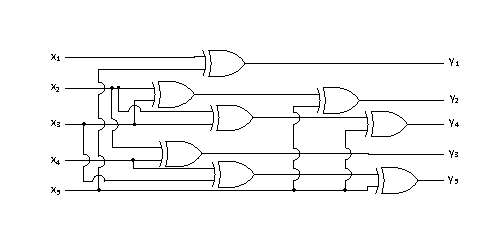
\includegraphics[scale=0.8]{./chapter_optimize/cse.pdf}
%     \label{fig:linearCircuita}
% }
% \subfigure[Equivalent cancellation-free linear circuit]{
%     % \rule{2cm}{3cm}
%     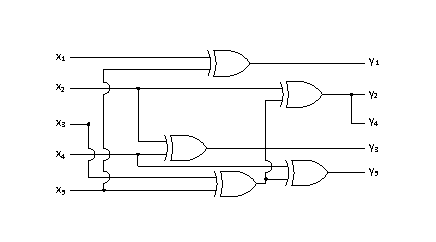
\includegraphics[scale=0.8]{./chapter_optimize/cse_opt.pdf}
%     \label{fig:linearCircuitb}
% }
% \caption{Two linear circuits that compute the same function. The left circuit is unoptimized and the right circuit is fully factored (cancellation-free).}
% \end{figure}

In 2009, Daniel Bernstein \cite{Bernstein09-1} published another algorithm for optimizing software implementations of linear maps modulo $2$ (i.e. linear forms with coefficients in $\mathbb{F}_2$). The main idea of this algorithm is as follows: given the linear forms $L_0,L_1,\dots,L_{q-1}$, input vector $x$ and output vector $y$, both of length $q$, compute the $q$ dot products $L_0 \cdot x$, $L_1 \cdot x$, \dots, $L_{q-1} \cdot x$, where $L_0 \geq L_1 \geq \dotsb \geq L_{q-1}$ and store the results in the coordinates of $y$. Motivated by the Bos-Coster approach \cite{Rooji95-1}, the algorithm recursively computes $(L_0 - L_1) \cdot x, L_1\cdot x,\dots, L_{q-1}$ and then adds $y_1$ into $y_0$ (i.e. $y_0 + y_1 = L_0 - L_1 + L_1 = L_0$). A modified description of the algorithm is given in Algorithm \ref{alg:bernsteinLinearOpt}.

\begin{algorithm}[ht!] %[htb]
\caption{Bernstein recursive optimization (transcribed from \cite{Bernstein09-1})} \label{alg:bernsteinLinearOpt}
\begin{algorithmic}[1]
	\Require $q$ Linear forms $L_0,L_1,\dots,L_{q-1}$, each of length $p$, and input and output vectors $x$ and $y$ such that $|x| = |y| = q$
	\If {$q = 0$}
		\State Stop.
	\EndIf
	\If {$p = 0$}
		\State Generate code that sets $y_i = 0$ for all $0 \leq i \leq q-1$.
		\State Stop.
	\EndIf
	\State Find $j \in \{0,1,\dots,q-1\}$ that maximizes $L_j$ in reverse lexicographical order.
	\If {$L_j[p-1] = 0$}
		\State Recurse with $L_k' = (L_k[0],\dots,L_k[p-2])$ for each $k = 0,1,\dots,q-1$.
		\State Stop.
	\EndIf
	\If {$q \geq 2$}
		\State Find $i \in \{0,1,\dots,q-1\} \setminus \{j\}$ that maximizes $L_i$ in reverse lexicographical order.
		\If {$L_i[p-1] = 1$}
			\State Recurse with $L_k' = L_k$ for all $k \in \{0,1,\dots,q-1\}$ and $L_j' = L_j \oplus L_i$, and ``insert'' one
			XOR gate that adds $x_i$ and $x_j$ and stores the result in $x_j$.
			\State Stop.
		\EndIf
		\State Recurse with $L_k' = L_k$ for each $k = 0,1,\dots,q-1$ except that $L_j'[p-1] = 0$, and ``insert'' one
		XOR gate that adds $x_{p-1}$ into output bit $y_j$.
		\State Stop.
	\EndIf
\end{algorithmic}
\end{algorithm}

For $16 \times 16$ matrices, Bernstein reported that the average cost after zero elimination, divided by $16 \times 16 = 256$, was $0.2694$, meaning that the average cost for a $16 \times 16$ matrix multiplication over $GF(2)$ was $16 \times 16 \times 0.2694 = 68.9664$ XOR gates, which is more than the reported $59.1$ average from Paar's technique. In general, our experiments confirm that, on average, Bernstein's technique yields linear programs with a larger number of gates than Paar's greedy factorization technique. 

Boyar and Peralta \cite{Boyar12-1} introduced another heuristic in 2012, which appears to offer the best results since Paar's technique. At a high level, the algorithm greedily searches for the smallest linear circuit that is equivalent to the input set of linear forms by building new linear combinations of functions from a set of ``known'' functions. More formally, the algorithm works by continually decreasing the distance $\delta(S, f)$, which is the minimum number of additions from functions in $S$ necessary to obtain the predicate $f$, for each $f_0,\dots,f_{n-1}$, where $f_0,\dots,f_{n-1}$ are the $n$ linear forms being optimized. The original ``base'' of $S$ consists of the functions corresponding to the predicate variables $x_0,\dots,x_{n-1}$. The algorithm iterates while the $\delta(S, f_i) \not= 0$ for all $0 \leq i \leq n-1$, and at each iteration adds a new base function $S_{\mu} = S_i + S_j$ for some pair of base functions $S_i$ and $S_j$ to $S$, updates the distances $\delta(S, f_i)$ for all $0 \leq i \leq n - 1$, and then repeats. The selection of $S_i$ and $S_j$ is made such that the new distances are minimized, where ties are handled according to one of the following rules:
\begin{enumerate}
	\item Maximize the Euclidean norm of the vector of distances.
	\item Maximize the square of the Euclidean norm minus the largest distance.
	\item Maximize the square of the Euclidean norm minus the difference of the largest two distances.
	\item With probability $p = 0.5$ select the first possible base pairs out of the set of possibilities, and with probability
	$1 - p = 0.5$ apply the Euclidean norm rule and choose the largest one.
\end{enumerate}

In cases where optimal linear programs are needed, these heuristic-based approximations are not always effective. Fuhs and Schneider-Kamp \cite{Fuhs10-1} were able to cleverly encode a linear program of length $k$ for set of linear forms $f_1,\dots,f_m$ into first order propositional logic. If a satisfiable model for the equivalent Boolean formula $\phi$ exists, then the shortest linear program is easily reconstructed from the model. Otherwise, there does not exist a straight line linear program of length $k$ that computes the $m$ linear forms. 

For a system of $m$ linear forms with input coefficients represented with a binary matrix $\mathbf{A}$, the optimal length $k^*$ of an equivalent straight line linear program lies in the closed interval $[m, |\mathbf{A}|_1 - m - 1]$. Using this fact and the provably correct method to determine if a linear program of length $k$ exists for a particular set of linear forms, the authors then search for the optimal solution by iteratively applying the SAT solver technique for consecutive values of $k$ in decreasing order until an unsatisfiable instance is found. Once this limit is reached, the optimal value of $k^*$ must be then $k + 1$.

This technique was tested on the upper and lower linear transformations that make Boyar and Peralta's area-efficient S-box. It was able to verify their $k^* = 23$ linear program length presented in \cite{Boyar12-1}. While, the $k = 20$ case is trivially shown to be unsatisfiable due to the pigeonhole principle, the SAT instance for $k \in \{21, 22\}$ proved to be too difficult for modern SAT solvers to solve, even with various preprocessing and tuning techniques presented in the paper. Since replicating this work and implementing this procedure is nontrivial, we leave the experimentation with this technique on the matrix candidates in this work to future work. 

\subsection{Improving Linear Circuit Minimization Efficiency}
We implemented the previously discussed algorithms in our circuit optimization library and tested the results of each one for $16 \times 16$ and $32 \times 16$ matrices, which are of interest in this work. Our results, which are summarized in Table \ref{tab:algComparison}, clearly show that the Boyar-Peralta heuristic optimization technique yields the smallest values for all cases with little difference between the four different tie breaking rules. 
\begin{table}
\caption{Comparison of different optimization algorithms for the target $16 \times 16$ and $32 \times 16$ matrices in this work. The average XOR counts were gathered by populating the entries of matrices with nonzero entries with probability $p = 0.5$ over a series of $500$ trials.}
\label{tab:algComparison}
\begin{center}
	\begin{tabular}{| c | c | c |} \hline
		\emph{Matrix Size} & \emph{Algorithm} & \emph{Average XOR Count} \\ \hline
		$16 \times 16$ & Paar Factorization & 58.14 \\
		$16 \times 16$ & Boyar-Peralta Optimization \#1 & 50.09 \\
		$16 \times 16$ & Boyar-Peralta Optimization \#2 & 50.11 \\
		$16 \times 16$ & Boyar-Peralta Optimization \#3 & 50.09 \\
		$16 \times 16$ & Boyar-Peralta Optimization \#4 & 53.1 \\
		$16 \times 16$ & Bernstein Optimization & 85.0 \\ \hline
		$32 \times 16$ & Paar Factorization & 103.89 \\
		$32 \times 16$ & Boyar-Peralta Optimization \#1 & 83.22 \\
		$32 \times 16$ & Boyar-Peralta Optimization \#2 & 83.27 \\
		$32 \times 16$ & Boyar-Peralta Optimization \#3 & 83.22 \\
		$32 \times 16$ & Boyar-Peralta Optimization \#4 & 88.15 \\
		$32 \times 16$ & Bernstein Optimization & 146.66 \\ \hline
	\end{tabular}
\end{center}
\end{table}

While these heuristic-based optimization techniques may come close to optimal solutions, doing so is not guaranteed. In the context of cryptographic applications, Canright was the first to utilize an exhaustive, tree-based search for optimal cancellation-free linear programs \cite{Canright05-1}. The algorithm works by recursively inserting a new variable $x_{\mu} = x_i + x_j$ for all pairs of variables $x_i$ and $x_j$ that are shared by more than one linear form and returning the selection that yields the smallest number of gates. We give a complete description of the procedure in Algorithm \ref{alg:exhaustiveCanright}. Due to the combinatorial complexity of the algorithm, it is difficult to quantify its exact running time. 

\begin{algorithm}[ht!] %[htb]
\caption{SequentialExhaustiveFactor($M$, $m$, $g$)} \label{alg:exhaustiveCanright}
\begin{algorithmic}[1]
	\State $g' \gets g$
	\For{$i = 0 \to m - 1$}
		\For{$j = 0 \to m$}
			\State $coli \gets $GETCOLUMN$(M, i)$
			\State $colj \gets $GETCOLUMN$(M, j)$
			\If{HW$(coli $ \& $ colj) > 1)$}
				\State $M' \gets COPY(M)$
				\State $newcol \gets maxcoli $ \& $ maxcolj$
				\State $wt \gets $HW($newcol)$
				\State PUTCOLUMN$(M', newcol, m + 1)$
				\State PUTCOLUMN$(M', $NEGATE$(newcol $ \& $ maxcoli), maxi)$
				\State PUTCOLUMN$(M', $NEGATE$(newcol $ \& $ maxcolj), maxj)$
				\State $gc \gets $SequentialExhaustiveFactor$(M', m+1, g - wt + 1)$
				\If {$gc < g'$}
					\State $g' \gets gc$
				\EndIf
			\EndIf
		\EndFor
	\EndFor
	\State \Return $g'$ 
\end{algorithmic}
\end{algorithm}

The only optimizations applied to this algorithm were elementary pruning techniques to avoid redundant tree branches. To our knowledge, no one has explored parallel implementations of this algorithm. Therefore, this is a fruitful opportunity to increase the dimension of matrices which can be fully optimized, thereby aiding our optimization step for $16 \times 16$ matrices. The parallel implementation of the algorithm, written in Java, makes use of the fork/join parallel programming pattern to perform a breadth first traversal of the matrix factorization tree. The algorithm is driven by a collection of worker threads which retrieve matrices from a pool of those discovered during the breadth-first traversal of the tree. The worker threads are managed by the Java ForkJoinPool service which execute an {\tt optimize()} method in a class entitled ParallelMatrixOptimize. A thorough snippet of the source code for the parallel factorization program is shown in Appendix \ref{app:sourceCode}, and the pseudocode description of the entire parallel algorithm is presented in Algorithm \ref{alg:parallelOptimize}.

\begin{algorithm}[ht!] %[htb]
\caption{ParallelExhaustiveFactor($M$, $m$, $g$)} \label{alg:parallelOptimize}
\begin{algorithmic}[1]
	\State $g' \gets g$
	\State $P \gets []$
	\For{$i = 0 \to m - 1$}
		\For{$j = 0 \to m$}
			\State $coli \gets $GETCOLUMN$(M, i)$
			\State $colj \gets $GETCOLUMN$(M, j)$
			\If{HW$(coli $ \& $ colj) > 1)$}
				\State $P \gets Append(P, (i, j))$
			\EndIf
		\EndFor
	\EndFor
	\State $T \gets []$
	\For{$(i, j) \in P$}
		\State $M' \gets COPY(M)$
		\State $newcol \gets maxcoli $ \& $ maxcolj$
		\State $wt \gets $HW($newcol)$
		\State PUTCOLUMN$(M', newcol, m + 1)$
		\State PUTCOLUMN$(M', $NEGATE$(newcol $ \& $ maxcoli), maxi)$
		\State PUTCOLUMN$(M', $NEGATE$(newcol $ \& $ maxcolj), maxj)$
		\State $T \gets Append(T, (M', m + 1, g - wt + 1))$
	\EndFor
	\State $R \gets invokeAll(ParallelExhaustiveFactor(T))$
	\For {$r \in R$}
		\If {$r.gc < g'$}
			\State $g' \gets r.gc$
		\EndIf
	\EndFor
	\State \Return $g'$ 
\end{algorithmic}
\end{algorithm}

We present a comparison of the performance against the Canright's sequential version (translated from his C program to Java) and our parallel factorization algorithm in Table \ref{tab:factorTimes}. On average, factoring matrices larger than $10 \times 10$ and $14 \times 7$ took an unreasonable amount of time to finish for the purpose of this experiment, as insinuated by Canright \cite{Canright05-1}. This led us to not pursue any further techniques for optimizing this particular algorithm. As a result, an exhaustive factorization for $16 \times 16$ and $32 \times 16$ matrices, which are the focus in this work, needed to be done with different and more efficient optimization techniques.

\begin{table}
\label{tab:factorTimes}
\caption{Comparison of the factorization time using the sequential and parallel factorization programs. }
\begin{center}
	\begin{tabular}{| c | c | c |} \hline
	$m \times n$ & \emph{Sequential Time (msec)} & \emph{Parallel Time (msec)} \\ \hline
	$7 \times 7$ & 16 & 15 \\ 
	$8 \times 8$ & 16 & 17 \\ 
	$9 \times 9$ & 188 & 79 \\ 
	$10 \times 10$ & 4625 & 1703 \\ 
	$12 \times 6$ & 9 & 9 \\
	$14 \times 7$ & 247 & 93 \\ \hline
	\end{tabular}
\end{center}
\end{table}

In addition to parallelizing the exhaustive factoring algorithm, we also implemented a parallel version of Boyar and Peralta's technique using the Parallel Java library \cite{Kaminsky10-1}. During the course of our preliminary experiments we observed that the computation of $\delta(S, f)$ was responsible for a large portion of program's overall execution time. Therefore, to speed up this computation, our parallel version of this technique evenly distributes and performs computation of $\delta(S, f)$ using multiple threads on an shared-memory multiprocessor (SMP) machine, thus enabling faster speedups as the dimension of the input set of linear forms increases (small sets of linear forms suffer from overhead of the parallel computing framework - i.e. thread team configuration and synchronization). See Appendix \ref{app:sourceCode} for a snippet of the source code for this program.

To study the performance gains of the parallel equivalents of this algorithm, we first denote the input problem size $N$ as the number of elements in the matrix representing the linear forms, $T$ as the execution time for a particular program run, and $K$ as the number of processors available for computation. We define sizeup as the ratio of the problem size solved for a given execution time to the number of processors available for computation, captured below as
\begin{align*}
Sizeup(T,K) = N_{par}(T,K) / N_{seq}(T,1)
\end{align*}
Similarly, we define speedup as the ratio of the problem execution time for a given problem size to the number of processors available for computation, captured below as
\begin{align*}
Speedup(N, K) = T_{seq}(N, K) / T_{par}(N, K)
\end{align*}
Since both sizeup and speedup are important when scaling up to $16 \times 16$ and $32 \times 16$ matrices, we measured each for $K = 1$, $2$, $3$, $4$, and $8$ processors to see how the parallel implementations scaled and approached the limit imposed by Amdahl's law. The results from these experiments for the first tie breaker in Boyar and Peralta's technique on an eight-processor SMP machine with with four UltraSPARC-IV dual-core processors, a 1.35 GHz clock frequency, and 16 GB of main memory are shown in Figures \ref{fig:speedup1}, \ref{fig:speedup2}, \ref{fig:sizeup1} and \ref{fig:sizeup2}. Notice that, although we appear to achieve efficient speedups limited by Amdahl's law, our the parallel implementations do not achieve efficient sizeups. This is an indication that running these programs on larger problems may not yield improved running times. Even still, our results show significant improvements for the $16 \times 16$ and $32 \times 16$ matrices that are the focus of this work, thus enabling us to process many more linear programs in a shorter amount of time. As a result, these parallel implementations should prove useful for related research. 

\begin{figure}
\begin{center}
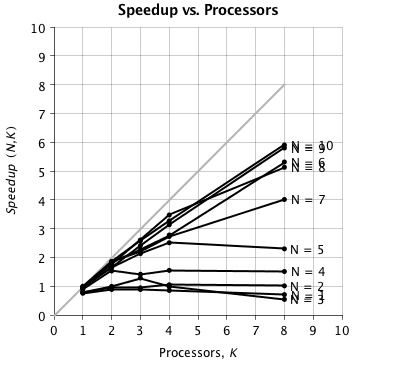
\includegraphics[scale=0.35]{./chapter_optimize/t1u_speed_3.png}
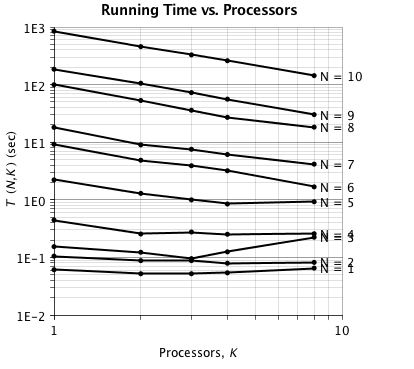
\includegraphics[scale=0.35]{./chapter_optimize/t1u_speed_4.png}
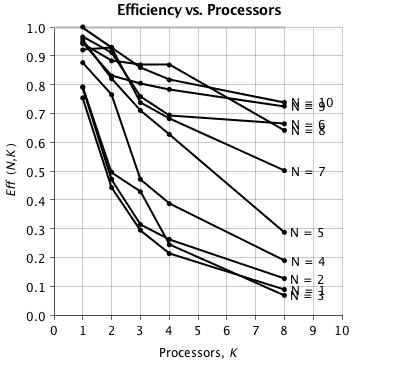
\includegraphics[scale=0.35]{./chapter_optimize/t1u_speed_2.png}
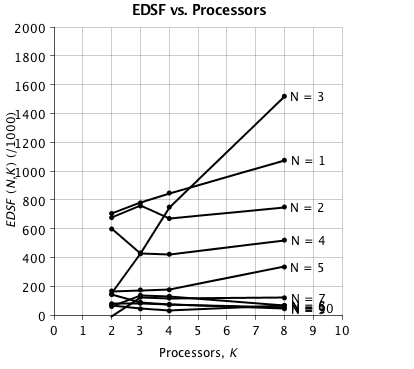
\includegraphics[scale=0.35]{./chapter_optimize/t1u_speed_1.png}
\caption{Speedup metrics for the parallel implementation of Boyar and Peralta's technique using tie breaker \#1 with $16 \times 16$ matrices. In these graphs we use $N = 1$ to denote $7 \times 7$ matrices, $N = 2$ to denote $8 \times 8$ matrices, etc.}
\label{fig:speedup1}
\end{center}

\begin{center}
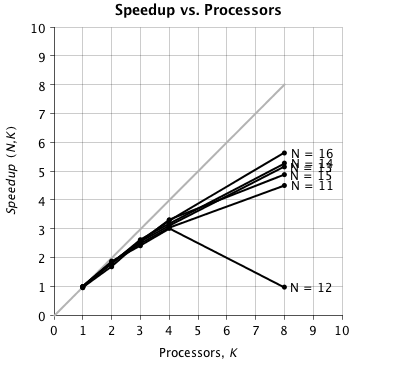
\includegraphics[scale=0.35]{./chapter_optimize/t1m_4.png}
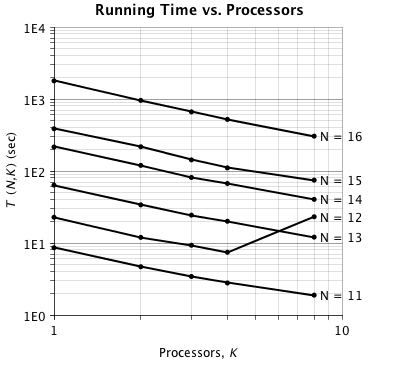
\includegraphics[scale=0.35]{./chapter_optimize/t1m_1.png}
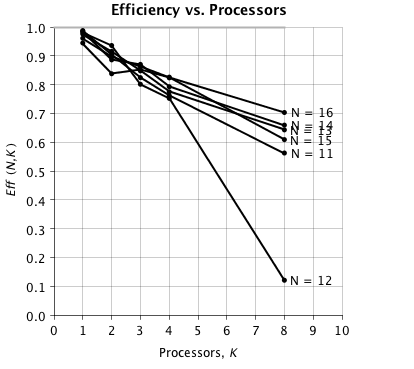
\includegraphics[scale=0.35]{./chapter_optimize/t1m_3.png}
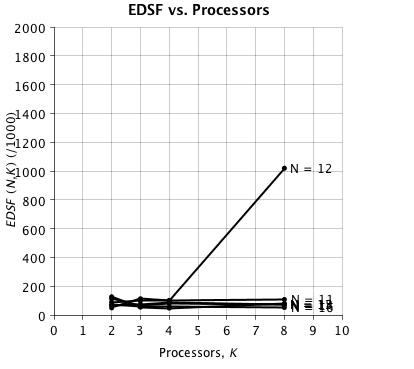
\includegraphics[scale=0.35]{./chapter_optimize/t1m_2.png}
\caption{Speedup metrics for the parallel implementation of Boyar and Peralta's technique using tie breaker \#1 with merged $32 \times 16$ matrices. In these graphs we use $N = 11$ to denote $22 \times 11$ matrices, $N = 2$ to denote $24 \times 12$ matrices, etc.}
\label{fig:speedup2}
\end{center}
\end{figure}

% \begin{figure}
% \begin{center}
% 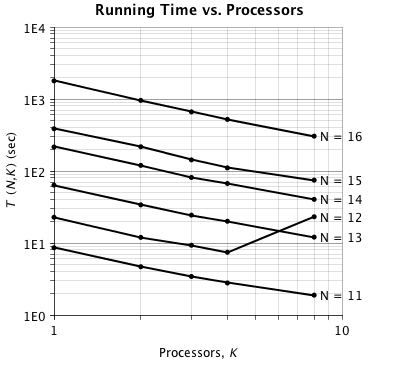
\includegraphics[scale=0.35]{./chapter_optimize/t1m_1.png}
% 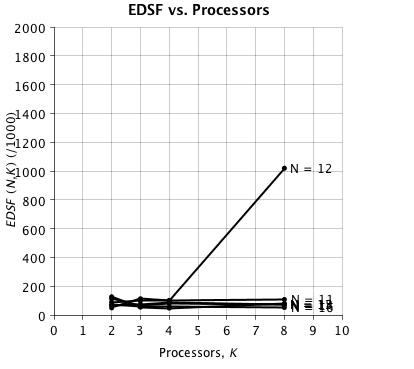
\includegraphics[scale=0.35]{./chapter_optimize/t1m_2.png}
% 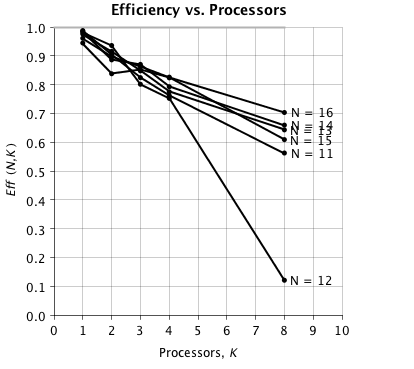
\includegraphics[scale=0.35]{./chapter_optimize/t1m_3.png}
% 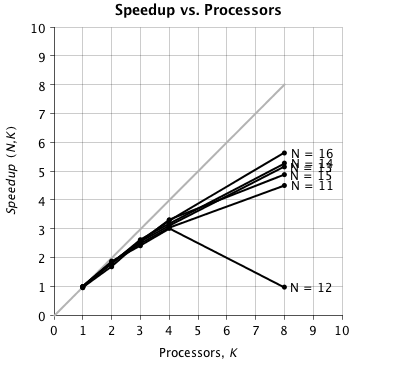
\includegraphics[scale=0.35]{./chapter_optimize/t1m_4.png}
% \caption{Speedup metrics for the parallel implementation of Boyar and Peralta's technique using tie breaker \#1 with merged $32 \times 16$ matrices.}
% \label{fig:speedup2}
% \end{center}
% \end{figure}

\begin{figure}
\begin{center}
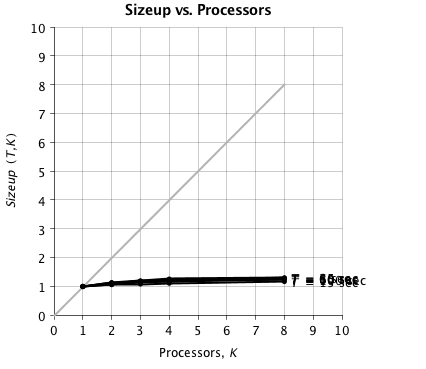
\includegraphics[scale=0.35]{./chapter_optimize/t1um_size_2.png}
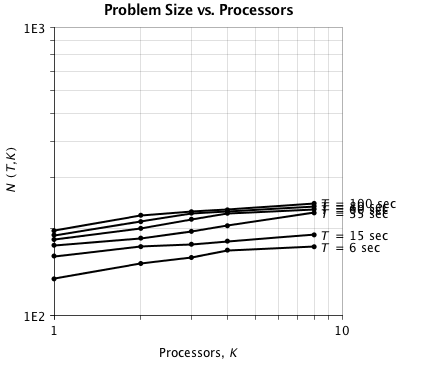
\includegraphics[scale=0.35]{./chapter_optimize/t1um_size_3.png}
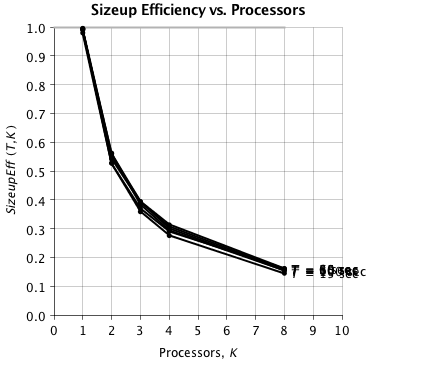
\includegraphics[scale=0.35]{./chapter_optimize/t1um_size_1.png}
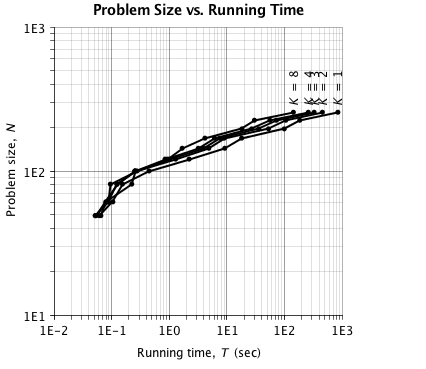
\includegraphics[scale=0.35]{./chapter_optimize/t1um_size_4.png}
\caption{Sizeup metrics for the parallel implementation of Boyar and Peralta's technique using tie breaker \#1 with merged $16 \times 16$ and unmerged matrices. This data was collected by running tests for matrices of size $7 \times 7$ to $16 \times 16$ matrices.}
\label{fig:sizeup1}
\end{center}

\begin{center}
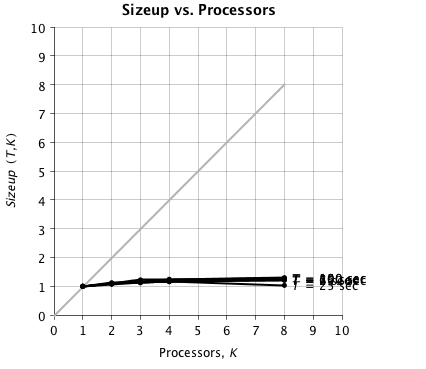
\includegraphics[scale=0.35]{./chapter_optimize/t1m_size_2.png}
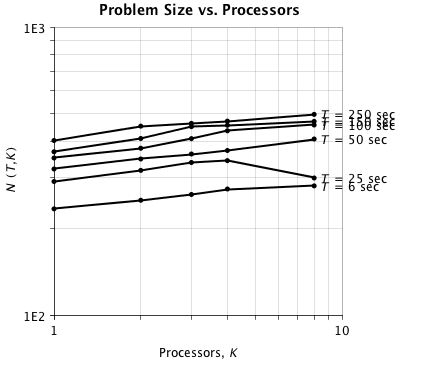
\includegraphics[scale=0.35]{./chapter_optimize/t1m_size_3.png}
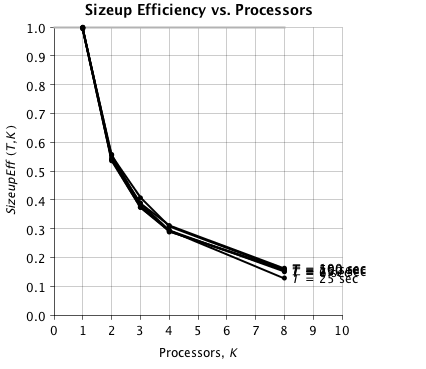
\includegraphics[scale=0.35]{./chapter_optimize/t1m_size_1.png}
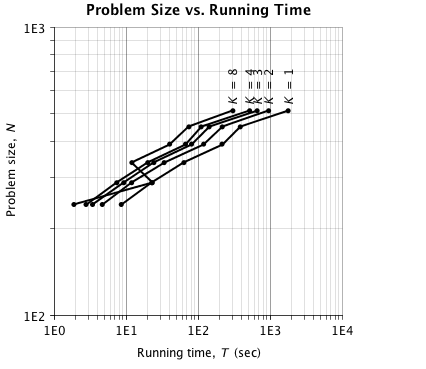
\includegraphics[scale=0.35]{./chapter_optimize/t1m_size_4.png}
\caption{Sizeup metrics for the parallel implementation of Boyar and Peralta's technique using tie breaker \#1 with merged $32 \times 16$ and unmerged matrices. This data was collected by running tests for matrices of size $22 \times 11$ to $32 \times 16$ matrices.}
\label{fig:sizeup2}
\end{center}
\end{figure}

% \begin{figure}
% \end{figure}

% \begin{figure}
% \begin{center}
% 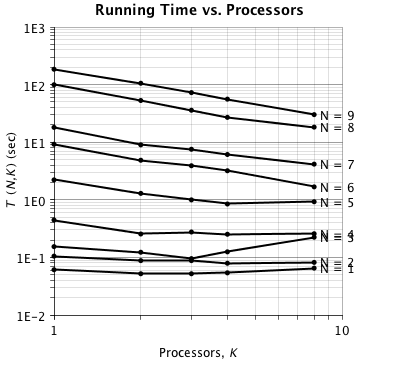
\includegraphics[scale=0.35]{./chapter_optimize/t1un_1.png}
% 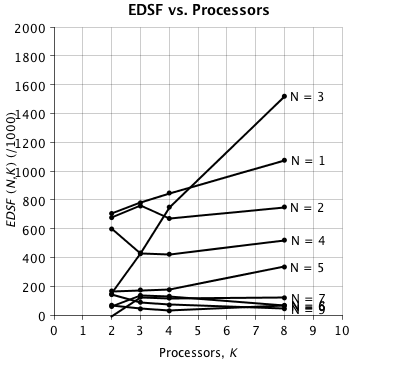
\includegraphics[scale=0.35]{./chapter_optimize/t1un_2.png}
% 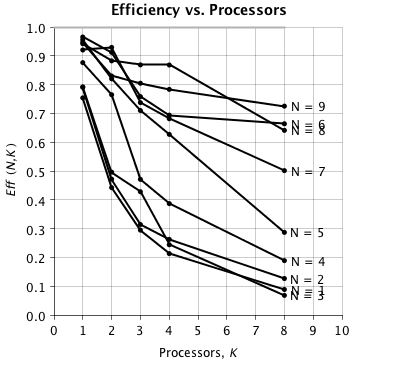
\includegraphics[scale=0.35]{./chapter_optimize/t1un_3.png}
% 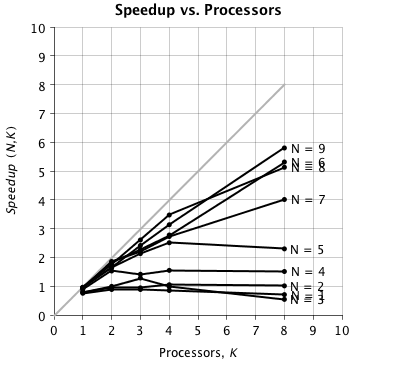
\includegraphics[scale=0.35]{./chapter_optimize/t1un_4.png}
% 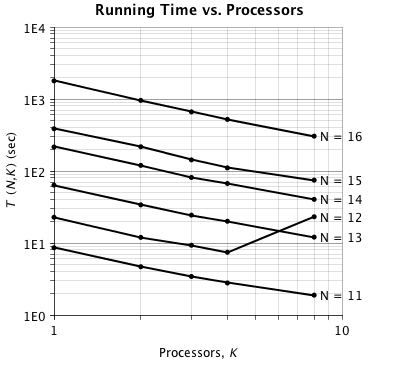
\includegraphics[scale=0.35]{./chapter_optimize/t1m_1.png}
% 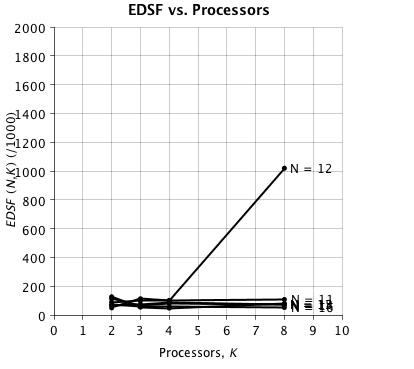
\includegraphics[scale=0.35]{./chapter_optimize/t1m_2.png}
% 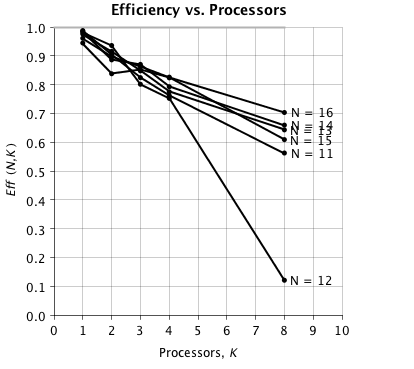
\includegraphics[scale=0.35]{./chapter_optimize/t1m_3.png}
% 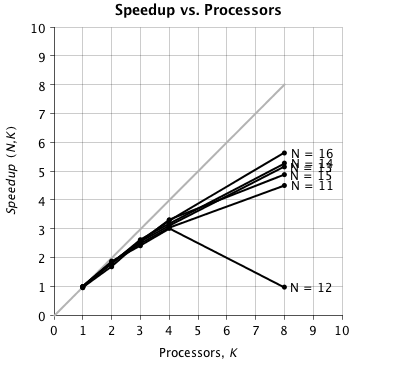
\includegraphics[scale=0.35]{./chapter_optimize/t1m_4.png}
% 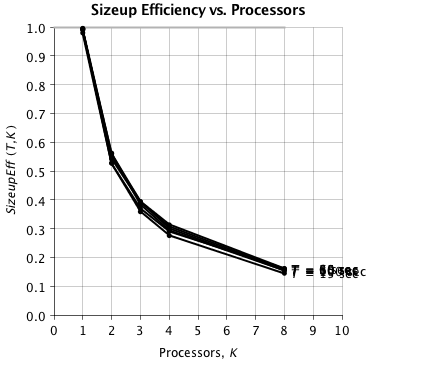
\includegraphics[scale=0.35]{./chapter_optimize/t1um_size_1.png}
% 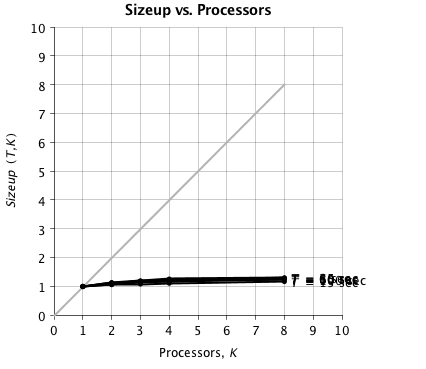
\includegraphics[scale=0.35]{./chapter_optimize/t1um_size_2.png}
% 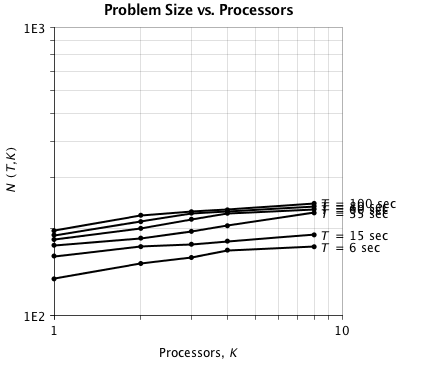
\includegraphics[scale=0.35]{./chapter_optimize/t1um_size_3.png}
% 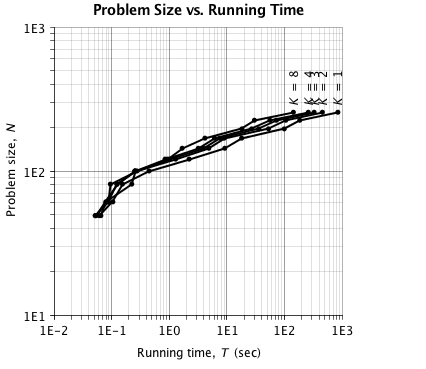
\includegraphics[scale=0.35]{./chapter_optimize/t1um_size_4.png}
% 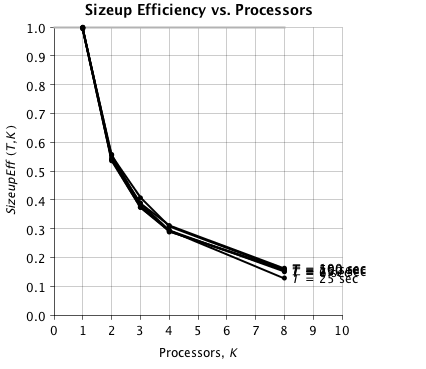
\includegraphics[scale=0.35]{./chapter_optimize/t1m_size_1.png}
% 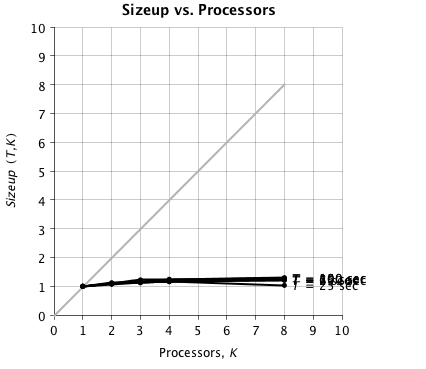
\includegraphics[scale=0.35]{./chapter_optimize/t1m_size_2.png}
% 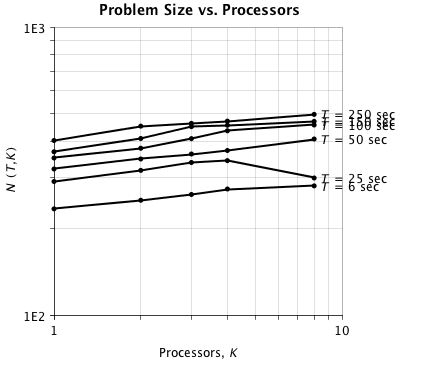
\includegraphics[scale=0.35]{./chapter_optimize/t1m_size_3.png}
% 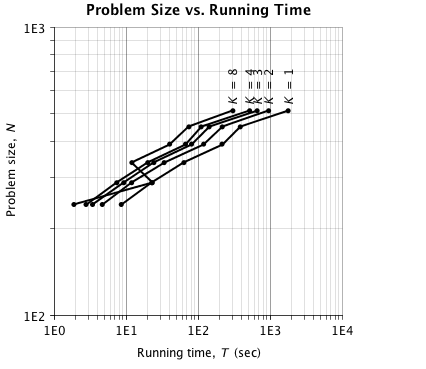
\includegraphics[scale=0.35]{./chapter_optimize/t1m_size_4.png}
% \caption{Speedup and sizeup metrics for the parallel implementation of Boyar and Peralta's technique using tie breaker \#2.}
% \label{fig:sizeup2}
% \end{center}
% \end{figure}

% \begin{figure}
% \begin{center}
% 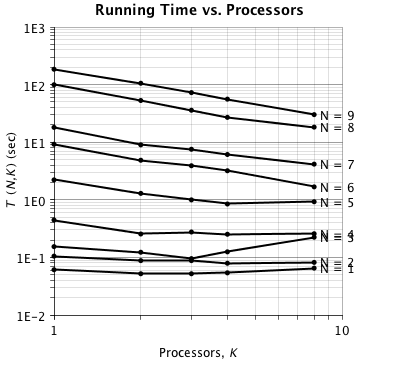
\includegraphics[scale=0.35]{./chapter_optimize/t1un_1.png}
% 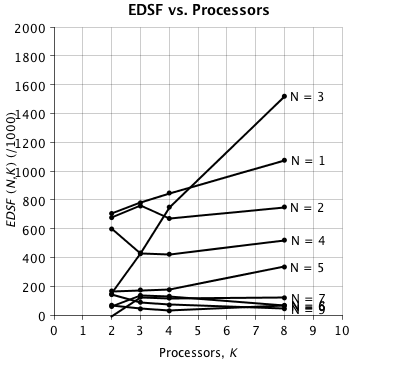
\includegraphics[scale=0.35]{./chapter_optimize/t1un_2.png}
% 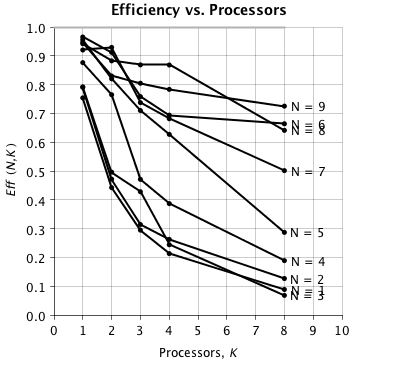
\includegraphics[scale=0.35]{./chapter_optimize/t1un_3.png}
% 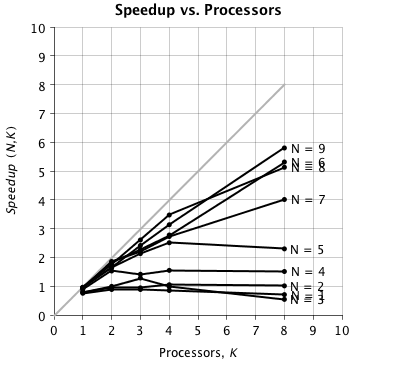
\includegraphics[scale=0.35]{./chapter_optimize/t1un_4.png}
% 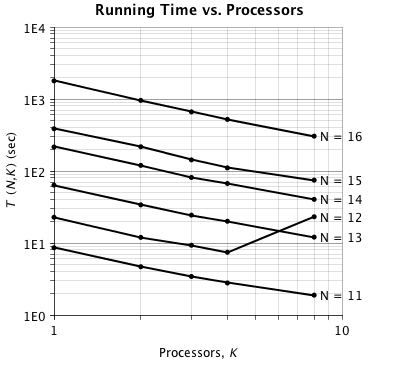
\includegraphics[scale=0.35]{./chapter_optimize/t1m_1.png}
% 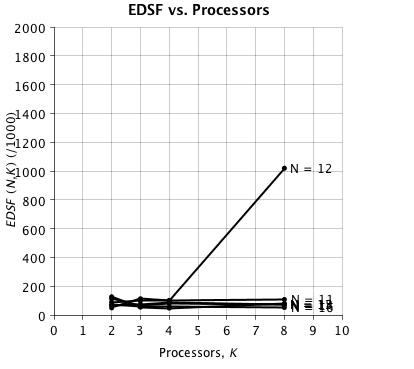
\includegraphics[scale=0.35]{./chapter_optimize/t1m_2.png}
% 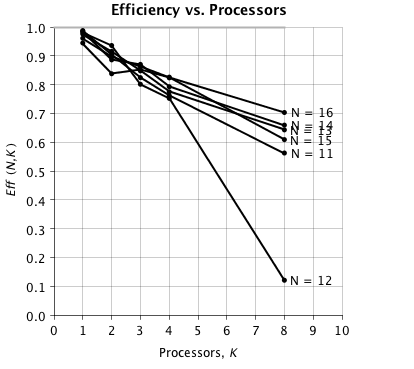
\includegraphics[scale=0.35]{./chapter_optimize/t1m_3.png}
% 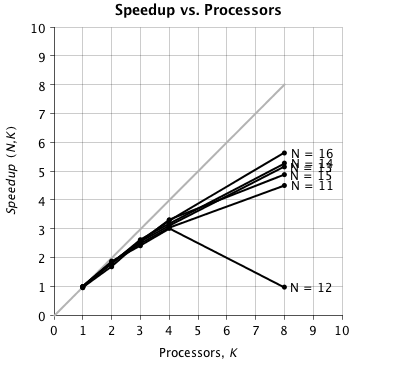
\includegraphics[scale=0.35]{./chapter_optimize/t1m_4.png}
% 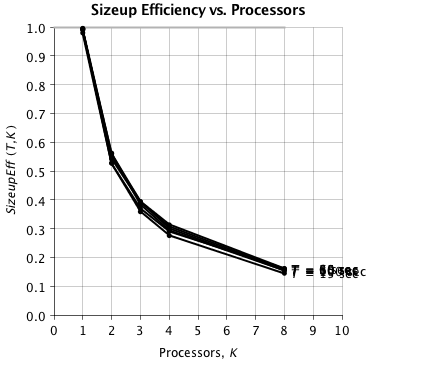
\includegraphics[scale=0.35]{./chapter_optimize/t1um_size_1.png}
% 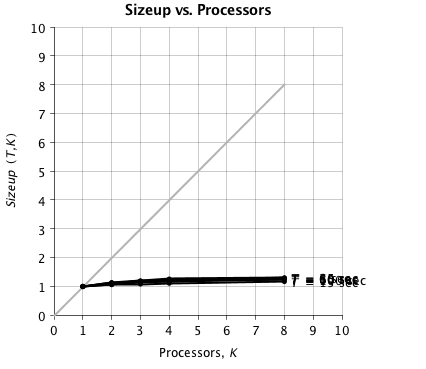
\includegraphics[scale=0.35]{./chapter_optimize/t1um_size_2.png}
% 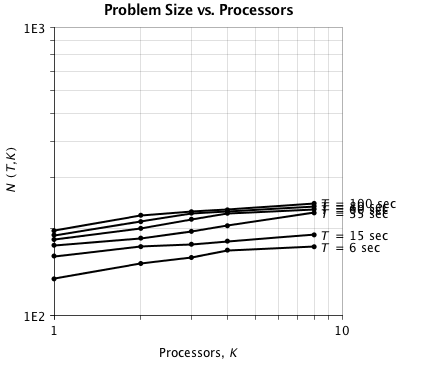
\includegraphics[scale=0.35]{./chapter_optimize/t1um_size_3.png}
% 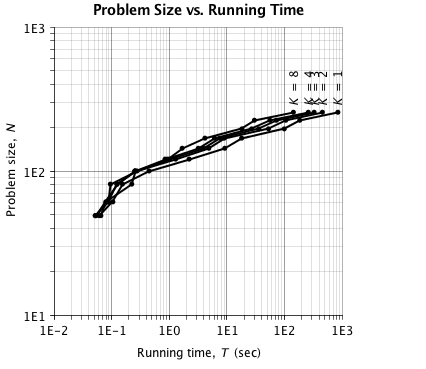
\includegraphics[scale=0.35]{./chapter_optimize/t1um_size_4.png}
% \includegraphics[scale=0.35]{./chapter_optimize/t1m_size_1.png}
% \includegraphics[scale=0.35]{./chapter_optimize/t1m_size_2.png}
% \includegraphics[scale=0.35]{./chapter_optimize/t1m_size_3.png}
% \includegraphics[scale=0.35]{./chapter_optimize/t1m_size_4.png}
% \caption{Speedup and sizeup metrics for the parallel implementation of Boyar and Peralta's technique using tie breaker \#3.}
% \label{fig:sizeup3}
% \end{center}
% \end{figure}

% \begin{figure}
% \begin{center}
% % \includegraphics[scale=0.35]{./chapter_optimize/s41.png}
% \includegraphics[scale=0.35]{./chapter_optimize/s42.png}
% \includegraphics[scale=0.35]{./chapter_optimize/s43.png}
% % \includegraphics[scale=0.35]{./chapter_optimize/s44.png}
% \caption{Speedup and sizeup metrics for the parallel implementation of Boyar and Peralta's technique using tie breaker \#4.}
% \label{fig:sizeup4}
% \end{center}
% \end{figure}

\newpage
\section{Optimizing Nonlinear Circuits}
While effective heuristics exist for optimizing linear circuits to reduce the number of required XOR gates, the problem becomes significantly more difficult if variables the straight line program can be multiplied together. As multiplication can usually be regarded as a more expensive operation than addition, we are generally interested in minimizing the number of multiplications required to compute a particular function. In NAND-based CMOS technology, AND/NAND gates are significantly cheaper than XOR gates because the former are used to build the latter. We disregard this detail for the purpose of working on the more general problem of minimizing the required multiplication operations, which is known as the \emph{multiplicative complexity}. In fact, this is the problem that motivated the two-step Boolean logic minimization technique pioneered by Boyar and Peralta \cite{Boyar12-1}. Shannon \cite{Shannon49-1} and Lupanov \cite{Lupanov58-1} showed that \emph{almost all} Boolean functions on $n$ inputs have a Boolean circuit complexity of about $\frac{2^n}{n}$, and Boyar et al. \cite{Boyar00-1} later showed that the common multiplicative complexity is $2^{n/2}$. Of course, these upper bounds do not hold for all Boolean functions, and as such, the problem of optimizing nonlinear circuits (or parts of a circuit) is related to the difficulty of attaining functions with polynomial multiplicative complexity. In this work we assume that the Boolean functions are not symmetric. That is, the output of such functions does not depend solely on the Hamming weight of the input. Given that this is a much more difficult problem to solve than symmetric Boolean functions \cite{Boyar00-1}, the more effective techniques for finding minimal nonlinear circuits have been randomized, heuristic-based searches. In the following section we describe some relevant techniques that have been applied in the context of cryptography and discuss our modifications on multiplicative inversion circuits for $GF(2^4)$.

% \todo[inline]{State the goal as trying to minimize the...}
% \todo[inline]{Discussion of Shannon's Boolean complexity stuff and the upper bounds...}
% \todo[inline]{Overview of peralta's technique and difficulty of the problem}
% \todo[inline]{Discussion of my heuristic varying number of XOR rounds and AND rounds...}

\subsection{Ad-Hoc Heuristics}
Perhaps the most effective heuristic to date for optimizing small nonlinear components of large circuits is the ad-hoc search heuristic developed by Boyar and Peralta \cite{Boyar12-1}. Inspired by techniques from automatic theorem proving, the core of their algorithm tries to construct an equivalent small area and low depth function for a given input function. Boyar and Peralta refer to the input columns of the truth table for a Boolean function $f$ as \emph{known signals}, and the output column of the same truth table as the signal of $f$. Then, for any two known signals $u$ and $v$ for functions $g$ and $h$, the sum $u \oplus v$ (product $u \land v$) is equivalent to the signal of the function $g \oplus h$ ($g \land h$). 

Their ad-hoc optimization algorithm wraps this function construction technique with a randomized search for an optimal function $g$ that is equivalent to the input function $f$ but has a lower multiplicative complexity. The iterations of this search are then divided into XOR and AND rounds, each of which will randomly select a specified number of signal pairs $(u, v)$ from the signal set of a working function $f$ and then compute their sum or product, depending on the type of round. Then, the algorithm checks to see if the resulting function $u \oplus v$ or $u \land v$ is equivalent to the input function $f$, and if so, returns the result as $g$. Otherwise, the new function is added to the set of known signals for the working function and the rounds continue. If at any point the number of AND gates exceeds a given threshold, or if the size of the known signal set exceeds a predefined depth, then the randomized algorithm restarts. 

This general procedure is followed for all input functions $f_1,\dots,f_n$, and in an effort to maximize signal reuse among each of the input functions, all of the signals computed during the XOR and AND rounds of a single function $f_i$ are saved for use optimizing all functions $f_j$, $j > i$. Since the functions that are stored vary depending on the order in the input functions $f_1,\dots,f_n$ are optimized, Boyar and Peralta tried all $n!$ permutations of the input set to find an optimized circuit for the nonlinear inversion circuit for $GF((2^2)^2)$ using the normal bases $[V, V^2]$ and $[W, W^4]$ (see the following chapter for more information). We modified and applied their optimization technique to the other $17$ inversion circuits for $GF((2^2)^2)$. The modifications include the ability to specify the number of gates added per AND/XOR round, as well as two evolving probabilities $p_x$ and $p_a$ that determine whether or not a gate is added in each round.

% We also developed our own heuristic that seeks to find an equivalent circuit for a set of linear
% forms by looking at the entire linear system at once, rather than iteratively trying to 
% construct one individual circuit at a time that reuses signals from previous iterations of 
% the algorithm. Our approach is inspired by the intuition that signals which are shared among
% more XOR and AND operations are preferred to those that are not shared. To maintain the 
% the ``fan-out'' of a particlar signal $u$, i.e. the number of signals that were created 
% using $u$, signals are created, stored, and updated as directed graphs representing where the source 
% vertices represent the input signals and the sink vertex represents the current signal ``value''.

% The algorithm for finding a circuit proceeds with XOR and AND rounds as in Boyar and
% Peralta's technique, with the additional operation of pruning the signal tree after a fixed number of 
% rounds. The pruning operation can apply a variety of heuristics for trimming the size of the tree 
% without removing those signals that have resulted in one of the $m$ output signals. The main strategy
% for removing signals in the tree is to remove the path in the tree that starts at a leaf node
% and has the maximum weight. We experimented with several other heuristics to test the effectiveness 
% of our approach, as shown in Figure \ref{fig:signalTreePrune}.
% \begin{figure}
% \begin{center}
% \includegraphics[scale=0.3]{./chapter_optimize/signal_graph.pdf}
% \caption{Visual depiction of several signal tree pruning strategies that were tried during our experiments.}
% \label{fig:signalTreePrune}
% \end{center}
% \end{figure}

\subsection{An Application to Small Galois Field Inversion Circuits}
Given the input and output size for the inversion circuits for $GF((2^2)^2)$, we may also forgo algebraic computations and implement direct inversion circuits that can be optimized using the combinational minimization technique discussed in the previous section. For example, suppose we want to compute the multiplicative inverse of an element in $GF((2^2)^2)$, which is defined by $p(v) = v^2 + v + 1$ and $q(w) = w^2 + w + v^2$. If elements in $GF(2^2)$ are represented using the normal basis $[V, V^2]$, and elements in $GF((2^2)^2)$ are represented in the normal basis $[W, W^4]$, then the inverse of $x$, $y = x^{-1}$, can be computed with the following nonlinear circuit \cite{Boyar12-1}.
\begin{align*}
y_1 & = x_2x_3x_4 + x_1x_3 + x_2x_3 + x_3 + x_4 \\
y_2 & = x_1x_3x_4 + x_1x_3 + x_2x_3 + x_2x_4 + x_4 \\
y_3 & = x_1x_2x_3 + x_1x_4 + x_1 + x_2 \\
y_4 & = x_1x_2x_3 + x_1x_1 + x_1x_4 + x_2x_4 + x_2
\end{align*}
There are $17$ other possible inversion circuits depending on the basis used for $GF(2^2)$ and $GF((2^2)^2)$ and the value of $\Sigma$ coefficient in the irreducible polynomial $q(w)$. For completeness, we list the $17$ circuits below. Some basis selections yield the same minimized circuits, and we group them together in such case, yielding only $8$ unique inversion circuits. For the first time we give complete circuits for all possible inversion circuits for mixed polynomial and normal basis representations of $GF((2^2)^2)$. 

% put in mofo newpage for -enhanced- readability... according to sam wise
\newpage
\begin{minipage}{.8\textwidth}

\hrule

\vspace{2em}
\noindent 
% Basis: $[V, V^2]$, $[W, W^4]$ \\
% Coefficient: $\Sigma = v$ \\
% Basis v v + 1 w w + 1 v
\textbf{Case}: 9 
% \vspace{-1em}
\begin{align*}
y_0 & = x_1 + x_0x_2 + x_0x_1x_2 + x_0x_3 + x_1x_3 \\
y_1 & = x_0 + x_1 + x_0x_2 + x_0x_3 + x_0x_1x_3 \\
y_2 & = x_0x_2 + x_1x_2 + x_3 + x_1x_3 + x_0x_2x_3 \\
y_3 & = x_2 + x_0x_2 + x_1x_2 + x_3 + x_1x_2x_3 \\
\end{align*}
\vspace{-1em}
\hrule
\vspace{2em}
\noindent 

\textbf{Cases}: 6 and 3
% Basis: $[V, V^2]$, $[1, w^4]$ \\
% Coefficient: $\Sigma = v$ \\
% Basis: $[V, V^2]$, $[1, W]$ \\
% Coefficient: $\Sigma = v$ \\
% \vspace{-1em}
\begin{align*}
y_0 & = x_1x_2 + x_3 + x_0x_2x_3 \\
y_1 & = x_2 + x_3 + x_0x_3 + x_1x_2x_3 \\
y_2 & = x_0 + x_0x_2 + x_1x_2 + x_0x_1x_2 + x_3 + x_0x_3 + x_1x_3 + x_0x_2x_3 \\
y_3 & = x_1 + x_2 + x_0x_2 + x_3 + x_0x_1x_3 + x_1x_2x_3 \\
\end{align*}
\vspace{-1em}


\hrule
\vspace{2em}
\noindent 

\textbf{Cases}: 8 and 16
% Basis: $[1, v^2]$, $[W, W^4]$\\
% Coefficient: $\Sigma = v$ \\
% Basis: $[1, v]$, $[W, W^4]$ \\
% Coefficient: $\Sigma = v + 1$ \\
% 1 v + 1 w w + 1 v
% \vspace{-1em}
\begin{align*}
y_0 & = x_0 + x_0x_2 + x_1x_2 + x_1x_3 + x_0x_1x_3 \\
y_1 & = x_1 + x_0x_2 + x_0x_1x_2 + x_0x_1x_3 \\
y_2 & = x_2 + x_0x_2 + x_0x_3 + x_1x_3 + x_1x_2x_3 \\
y_3 & = x_0x_2 + x_3 + x_0x_2x_3 + x_1x_2x_3 \\
\end{align*}
\vspace{-1em}


\hrule
\vspace{2em}
\noindent 

\textbf{Cases}: 5, 2, 13, and 10
% Basis: $[1, v^2]$, $[1, w^4]$ \\
% Coefficient: $\Sigma = v$ \\
% Basis: $[1, v^2]$, $[1, W]$ \\
% Coefficient: $\Sigma = v$ \\
% Basis: $[1, v]$, $[1, w^4]$ \\
% Coefficient: $\Sigma = v + 1$ \\
% Basis: $[1, v]$, $[1, W]$ \\
% Coefficient: $\Sigma = v + 1$ \\
% 1 v + 1 1 w + 1 v
% \vspace{-1em}
\begin{align*}
y_0 & = x_2 + x_0x_3 + x_1x_2x_3 \\
y_1 & = x_1x_2 + x_3 + x_0x_3 + x_0x_2x_3 + x_1x_2x_3 \\
y_2 & = x_1 + x_2 + x_0x_2 + x_1x_2 + x_0x_3 + x_1x_3 + x_0x_1x_3 + x_1x_2x_3 \\
y_3 & = x_0 + x_1 + x_0x_2 + x_1x_2 + x_0x_1x_2 + x_3 + x_0x_3 + x_0x_1x_3 + x_0x_2x_3 + x_1x_2x_3 \\
\end{align*}
\vspace{-1em}

\hrule

\end{minipage}
\newpage
\begin{minipage}{.8\textwidth}


\hrule
\vspace{2em}

\noindent 
\textbf{Cases}: 7 and 17
% Basis: $[1, v]$, $[W, W^4]$ \\
% Coefficient: $\Sigma = v$ \\
% Basis: $[1, v^2]$, $[W, W^4]$ \\
% Coefficient: $\Sigma = v + 1$ \\
 % 1 v w w + 1 v
% \vspace{-1em}
\begin{align*}
y_0 & = x_0 + x_1 + x_0x_2 + x_0x_3 + x_0x_1x_3 \\
y_1 & = x_0 + x_0x_1x_2 + x_1x_3 + x_0x_1x_3 \\
y_2 & = x_2 + x_0x_2 + x_1x_2 + x_3 + x_1x_2x_3 \\
y_3 & = x_2 + x_1x_3 + x_0x_2x_3 + x_1x_2x_3 \\
\end{align*}
\vspace{-1em}



\hrule
\vspace{2em}

\noindent 

\textbf{Cases}: 4, 1, 14, and 11
% Basis: $[1, v]$, $[1, w^4]$ \\
% Coefficient: $\Sigma = v$ \\
% Basis: $[1, v]$, $[1, W]$ \\
% Coefficient: $\Sigma = v$ \\
% Basis: $[1, v^2]$, $[1, w^4]$ \\
% Coefficient: $\Sigma = v + 1$ \\
% Basis: $[1, v^2]$, $[1, W]$ \\
% Coefficient: $\Sigma = v + 1$ \\
% 1 v 1 w + 1 v
% \vspace{-1em}
\begin{align*}
y_0 & = x_2 + x_3 + x_0x_3 + x_1x_2x_3 \\
y_1 & = x_2 + x_1x_2 + x_0x_3 + x_0x_2x_3 + x_1x_2x_3 \\
y_2 & = x_1 + x_2 + x_0x_2 + x_3 + x_0x_1x_3 + x_1x_2x_3 \\
y_3 & = x_0 + x_1 + x_2 + x_1x_2 + x_0x_1x_2 + x_0x_3 + x_1x_3 + x_0x_1x_3 + x_0x_2x_3 + x_1x_2x_3 \\
\end{align*}
\vspace{-1em}

\hrule
\vspace{2em}
\noindent 

\textbf{Cases}: 18
% Basis: $[V, V^2]$, $[W, W^4]$ \\
% Coefficient: $\Sigma = v + 1$ \\ 
 % v v + 1 w w + 1 v + 1
% \vspace{-1em}
\begin{align*}
y_0 & = x_0 + x_1 + x_1x_2 + x_0x_1x_2 + x_1x_3 \\
y_1 & = x_0 + x_0x_2 + x_1x_2 + x_1x_3 + x_0x_1x_3 \\
y_2 & = x_2 + x_3 + x_0x_3 + x_1x_3 + x_0x_2x_3 \\
y_3 & = x_2 + x_0x_2 + x_0x_3 + x_1x_3 + x_1x_2x_3 \\
\end{align*}
\vspace{-1em}

\hrule
\vspace{2em}
\noindent 

\textbf{Cases}: 15 and 12
% Basis: $[V, V^2]$, $[1, W^4]$ \\
% Coefficient: $\Sigma = v + 1$ \\
% Basis: $[V, V^2]$, $[1, W]$ \\
% Coefficient: $\Sigma = v + 1$ \\
 % v v + 1 1 w + 1 v + 1
% \vspace{-1em}
\begin{align*}
y_0 & = x_2 + x_1x_2 + x_3 + x_0x_2x_3 \\
y_1 & = x_2 + x_0x_3 + x_1x_2x_3 \\
y_2 & = x_0 + x_2 + x_0x_1x_2 + x_3 + x_1x_3 + x_0x_2x_3 \\
y_3 & = x_1 + x_2 + x_0x_2 + x_1x_2 + x_0x_3 + x_1x_3 + x_0x_1x_3 + x_1x_2x_3 \\
\end{align*}
\vspace{-1em}

\hrule

\end{minipage}
\newpage % so it's not ugly...

We optimized these $8$ distinct circuits for reduced area using a 120nm feature size library with the Synopsys ASIC design tool. To test the effectiveness of our modified Boyar-Peralta minimization technique, we compared the synthesis results from Synopsys generated using SLP representations of each circuit with this technique to the synthesis results generated from a typical Sum of Products (SOP) representation. More specifically, both representations for each of these circuits were translated to corresponding HDL and then synthesized using a Synopsys to obtain an approximate number of NAND gate equivalents (GEs). We list the results of these two techniques in Table \ref{tab:inverseCircuitMinimized}. We also include results for the three different inversion circuits for $GF(2^4)$ defined by the three unique irreducible polynomials $p(v) = v^4 + v + 1$, $p(v) = v^4 + v^3 + 1$, and $p(v) = v^4 + v^3 + v^2 + v + 1$ for elements in a polynomial basis. Note that different \emph{area} results might be achieved using a different CMOS technology. However, we expect the GEs to remain virtually the same in such cases. Also, since the Synopsys tool does not provide the ability to extract the number of logic gates used to implement a particular circuit after the synthesis task, we estimated the GEs by synthesizing and optimizing a single two-input NAND gate using the same cell size library. The result was a combinational area footprint of 1.0. Thus, to find the gate equivalents for a particular circuit, we simply read the total combinational area footprint. 

It is interesting to note that the smallest synthesized circuit for inversion in $GF((2^2)^2)$, which has a total of 20.50 GEs obtained with the SOP representation, is that which uses a polynomial basis $[1, V^2]$ for $GF(2^2)$ and normal basis $[W, W^4]$ for $GF((2^2)^2)$. The RTL schematic for this particular circuit, as synthesized in Synopsys, is shown in Figure \ref{fig:gf4BestInversea}. Interestingly, the inversion circuit for the field representation used in Canright's optimized S-box has $27.75$ GEs \cite{Canright05-1}. We leave the investigation of substituting this smaller inversion circuit into the $GF(2^8)$ and $GF(2^{16})$ inversion circuits for future work. It is also important to note that for every case the Synopsys tool was able to generate a smaller circuit using the SOP representation than the one obtained by our modified Boyar-Peralta minimization heuristic. Given the time constraints for this work, we were not able to explore the various optimizations and modifications to the algorithm that are noted in \cite{Boyar12-1}, and credit the discrepancies in the synthesis results from these two approaches to insufficient SLP optimizations.
\begin{figure}[ht]
\centering
\subfigure[Inversion circuit corresponding to cases 8 and 16 in Table \ref{tab:inverseCircuitMinimized}]{
    % \rule{2cm}{3cm}
    \includegraphics[scale=0.3]{./chapter_optimize/inverse22.png}
    \label{fig:gf4BestInversea}
}
\subfigure[Inversion circuit corresponding to case 20 in Table \ref{tab:inverseCircuitMinimized}]{
    % \rule{2cm}{3cm}
    \includegraphics[scale=0.25]{./chapter_optimize/inverse4.png}
    \label{fig:gf4BestInverseb}
}
\caption{RTL schematics for the smallest $GF((2^2)^2)$ and $GF(2^4)$ inversion circuits generated with the Synopsys tool.}
\end{figure}

% However, we have started collaborating with Peralta to explore such modifications in the future as part of the Circuit Minimization Team \cite{CMT}. 

\begin{table} 
\begin{center}
\scriptsize
	\caption{Hardware area requirements for a variety of inversion circuits for fields isomorphic to $GF(2^4)$. The Sum of Products (SOP) entries are unoptimized circuits derived directly from the corresponding truth table, and the optimized entries are those minimized using our modified version of the Boyar-Peralta technique.}
	\label{tab:inverseCircuitMinimized}
	\begin{tabular}{| c | c | c | c | c | c | } \hline  
	\emph{Case} & \emph{Field} & $q(w)$ & \emph{Bases} & \emph{SOP (GEs)} & \emph{Ad-Hoc Optimization (GEs)} \\ \hline
	1 & $GF((2^2)^2)$ & $w^2 + w + v$ & $[1, V]$ and $[1, W]$         & 26.00 & 51.5      \\
	2 & $GF((2^2)^2)$ & $w^2 + w + v$ & $[1, V^2]$ and $[1, W]$       & 27.25 & 49.75     \\
	3 & $GF((2^2)^2)$ & $w^2 + w + v$ & $[V, V^2]$ and $[1, W]$       & 31.50 & 44.0      \\
	4 & $GF((2^2)^2)$ & $w^2 + w + v$ & $[1, V]$ and $[1, W^4]$       & 26.00 & 51.5      \\
	5 & $GF((2^2)^2)$ & $w^2 + w + v$ & $[1, V^2]$ and $[1, W^4]$     & 27.25 & 49.75     \\
	6 & $GF((2^2)^2)$ & $w^2 + w + v$ & $[V, V^2]$ and $[1, W^4]$     & 31.50 & 44.0      \\
	7 & $GF((2^2)^2)$ & $w^2 + w + v$ & $[1, V]$ and $[W, W^4]$       & 22.75 & 36.75     \\
	8 & $GF((2^2)^2)$ & $w^2 + w + v$ & $[1, V^2]$ and $[W, W^4]$     & 20.50 & 22.25     \\
	9 & $GF((2^2)^2)$ & $w^2 + w + v$ & $[V, V^2]$ and $[W, W^4]$     & 27.75 & 37.5      \\
	10 & $GF((2^2)^2)$ & $w^2 + w + v^2$ & $[1, V]$ and $[1, W]$       & 27.25 & 49.75     \\
	11 & $GF((2^2)^2)$ & $w^2 + w + v^2$ & $[1, V^2]$ and $[1, W]$     & 26.00 & 51.5      \\
	12 & $GF((2^2)^2)$ & $w^2 + w + v^2$ & $[V, V^2]$ and $[1, W]$     & 29.00 & 41.75     \\
	13 & $GF((2^2)^2)$ & $w^2 + w + v^2$ & $[1, V]$ and $[1, W^4]$     & 27.25 & 49.75     \\
	14 & $GF((2^2)^2)$ & $w^2 + w + v^2$ & $[1, V^2]$ and $[1, W^4]$   & 26.00 & 51.5      \\
	15 & $GF((2^2)^2)$ & $w^2 + w + v^2$ & $[V, V^2]$ and $[1, W^4]$   & 29.00 & 41.75     \\
	16 & $GF((2^2)^2)$ & $w^2 + w + v^2$ & $[1, V]$ and $[W, W^4]$     & 20.50 & 22.25     \\
	17 & $GF((2^2)^2)$ & $w^2 + w + v^2$ & $[1, V^2]$ and $[W, W^4]$   & 22.75 & 36.75     \\
	18 & $GF((2^2)^2)$ & $w^2 + w + v^2$ & $[V, V^2]$ and $[W, W^4]$   & 29.25 & 34.75     \\
	19 & $GF(2^4)$ & $w^4 + w + 1$ & $[1, W, W^2, W^3]$                & 36.50 & NA  \\
	20 & $GF(2^4)$ & $w^4 + w^3 + 1$  & $[1, W, W^2, W^3]$             & 22.00 & NA  \\
	21 & $GF(2^4)$ & $w^4 + w^3 + w^2 + w + 1$  & $[1, W, W^2, W^3]$   & 26.00 & NA  \\ \hline
	
	% $GF(2^4)$ & $w^4 + w + 1$  & $[w^8, w^4, w^2, w]$             & RUNNING! & RUNNING! & RUNNING! \\
	% $GF(2^4)$ & $w^4 + w^3 + 1$  & $[w^8, w^4, w^2, w]$           & RUNNING! & RUNNING! & RUNNING! \\
	% $GF(2^4)$ & $w^4 + w^3 + w^2 + w + 1$ & $[w^8, w^4, w^2, w]$  & RUNNING! & RUNNING! & RUNNING! \\ \hline
	\end{tabular}
\end{center}
\end{table}


\chapter{Area-Optimized Implementations of the Galois Field Multiplicative Inverse} \label{chp:inverseImpl}
% It was shown by Nyberg \cite{Nyberg94-1} that the multiplicative inverse mapping
% $F(x) = x^{-1}$, where $x,x^{-1} \in GF(2^k)$ for some $k \geq 1$,
% has some important cryptographic properties that are ideal for 
% cryptographic S-boxes. In particular, Nyberg proved the following:
% \begin{enumerate}
% 	\item $\mathcal{N}_l \geq 2^{n-1} - 2^{n/2}$,
% 	\item $deg(\mathbf{Tr}(\omega x^{-1})) = w_2(2^n - 2) = n - 1$, 
% 	\item $F(x)$ is differentially $2$-uniform if $k$ is odd and differentially $4$-uniform if $k$ is even.
% \end{enumerate}
% Such properties are cited as the reason why this mapping was chosen as the basis for the Rijndael
% S-box \cite{Daemen02-1}. Additionally, it is well known that this mapping can be efficiently
% computed in polynomial time (Nyberg proposes the use of the Extended Euclidean Algorithm). 
% There are, however, many efficient algorithms for computing the multiplicative inverse 
% of an element in the field $GF(2^k)$, and in order to adequately quantify the implementation
% efficiency of a particular mapping, all such algorithms must be considered.

There are many methods for computing the multiplicative inverse of an element in a Galois field, including the well-known Extended Euclidean Algorithm, an application of Fermat's Little Theorem with the square and multiply algorithm for fast exponentiation, and most importantly, reduction to the inversion in the subfield. This work focuses on the latter technique. 

\section{Reduction to Subfield Inversion}
It is a well-known fact that computing the multiplicative inverse can be done by reducing the operation to those in subfields \cite{Itoh88-1, Paar95-1, Rijmen00-1}. There exists many isomorphic tower field representations of $GF(2^{16})$ that we can use in this reduction, all of which are shown in Figure \ref{fig:gfDecompose}. Depending on the algorithm used to decompose the multiplicative inverse calculation, certain tower field representations may be more or less optimal than others. To date, degree 2 extensions of $GF(2)$ have been shown to yield the smallest area S-boxes for the AES \cite{Canright05-1, Satoh01-1, Mentens05-1, Boyar11-1}. We follow this approach and select $GF((((2^2)^2)^2)^2)$ as the field isomorphic to $GF(2^{16})$. We also consider the fields $GF((2^8)^2)$, $GF((2^4)^2)$, and $GF((2^2)^8)$ in the context of the Itoh-Tsujii inversion algorithm (discussed later), though our preliminary results indicate that algebraic computations in tower fields of degree 2 extensions yield smaller area inversion circuits. 

\begin{figure}
\centering
\begin{tikzpicture}
[bend angle =60,inner sep=0pt, minimum size =10mm,very thick,
from/.style={<-},
towards/.style={->},
field/.style={}]
\node[field] (gf216) at (0,0) {$GF(2^{16})$};
\node[field] (gf282) at (-6,-2) {$GF((2^8)^2)$};
\node[field] (gf228) at (0,-2) {$GF((2^2)^8)$};
\node[field] (gf244) at (6,-2) {$GF((2^4)^4)$};
\node[field] (gf2422) at (-8,-4) {$GF(((2^4)^2)^2)$};
\node[field] (gf2422) at (-4,-4) {$GF(((2^2)^4)^2)$};
\node[field] (gf2224) at (4,-4) {$GF(((2^2)^2)^4)$};
\node[field] (gf22222) at (-6,-6) {$\mathbf{GF((((2^2)^2)^2)^2)}$};

\draw [->] (-1,-.25) -- (-5.75,-1.55);
\draw [->] (0,-.35) -- (0,-1.55);
\draw [->] (1,-.25) -- (5.75,-1.55);
\draw [->] (-6.75,-2.25) -- (-8,-3.75);
\draw [->] (-5.25,-2.25) -- (-4,-3.75);
\draw [->] (5.25,-2.25) -- (4,-3.75);
\draw [->] (-8,-4.5) -- (-6,-5.75);
\end{tikzpicture}
\caption{All possible tower field representations for $GF(2^{16})$. Our constructions use the isomorphic field $GF((((2^2)^2)^2)^2)$.}
\label{fig:gfDecompose}
\end{figure}

\subsection{Direct Inversion using Polynomial and Normal Bases}
Computing the multiplicative inverse of an element in $GF((((2^2)^2)^2)^2)$ can be done by systematically reducing the inversion computation to the subfield $GF(((2^2)^2)^2)$, which in turn reduces the inversion operation to the subfield $GF((2^2)^2)$, and so on. Ultimately, all arithmetic operations in $GF((((2^2)^2)^2)^2)$ operations reduce to bitwise operations in $GF(2)$, making algebraic decomposition a very effective strategy for constructing small area inversion circuits. 

To begin, we show that it is indeed possible compute the inverse of element $\alpha \in GF((2^n)^m)$, $\alpha^{-1}$, by solving the equation $\alpha\alpha^{-1} = 1$ for $\alpha^{-1}$. Before solving this equation, we first introduce some consistent notation. Let $t(z)$ be the degree $16$ irreducible polynomial that defines the field $GF(2^{16})$, $s(y) = y^2 + \Psi y + \Lambda$, be the irreducible polynomial that defines the field $GF((2^8)^2)$, $r(x) = x^2 + \Theta x + \Pi$ be the irreducible polynomial that defines the field $GF((2^4)^2)$, $q(w) = w^2 + \Omega w + \Sigma$ be the irreducible polynomial that defines the field $GF((2^2)^2)$, and finally $p(v) = v^2 + v + 1$ be the \emph{only} irreducible polynomial that defines the field $GF(2^2)$. Note that we enforce the $\Psi = \Theta = \Omega = 1$ so as to simplify all field arithmetic. 

% We refer the reader to Canright's derivations in \cite{Canright05-1} for a more thorough discussion of the rationale for this constraint. 

Furthermore, note that $\Psi, \Lambda \in GF(2^8)$, $\Theta, \Pi \in GF(2^4)$, and $\Omega, \Sigma \in GF(2^2)$. With this set of polynomials, it is clear that we can construct the field $GF((((2^2)^2)^2)^2)$ with the tuple of polynomials $(p(v), q(w), r(x), s(y))$. Finally, for consistency we will denote $\theta$ as an element in $GF(2^{16})$, $\zeta$ as an element in $GF(2^8)$, $\epsilon$ as an element in $GF(2^4)$, $\delta$ as an element in $GF(2^2)$, and $\gamma$ as an element in $GF(2)$ (i.e. a single bit). We now begin with the multiplicative inverse derivation for elements in each of the tower fields contained in $GF((((2^2)^2)^2)^2)$, starting with $GF(2^2)$, the first extensions field in the full tower. Computing the inverse in $GF(2^2)$ is trivial in both normal and polynomial bases. One may easily verify that for an element $\delta = \gamma_1 v + \gamma_2$ represented in the polynomial basis $[1,V]$, the inverse $\delta^{-1} = \gamma_1 v + (\gamma_1 + \gamma_2)$. If $\delta$ was represented using the normal basis $[V,V^2]$, then by Fermat's Little Theorem we have that $\delta^{-1} = \delta^2$, so $\delta^{-1} = (\gamma_1 v^2 + \gamma_2v)^2 = (\gamma_2 V^2 + \gamma_1V)$.

Computing the inverse of an element $\epsilon \in GF((2^2)^2)$, $\epsilon = \delta_1 w + \delta_2$, represented in a polynomial basis is not as trivial as in the previous computation. We derive a simplified expression for the inverse $\epsilon^{-1}$, $\epsilon = \delta_3 w + \delta_4$ using operations in the subfield $GF(2^2)$ by solving the equation $\epsilon\times\epsilon^{-1} = 1$ as follows:
\begin{align*}
\epsilon\times\epsilon^{-1} = & (\delta_1 w + \delta_2)(\delta_3 w + \delta_4) \\
= & \delta_1\delta_3 w^2 + \delta_1\delta_4 w + \delta_2\delta_3 w + \delta_2\delta_4 \\
= & k(w^2 + w + \Sigma) + 1 \\
= & 1,
\end{align*}
for some $k \in \mathbb{Z}$. If we match coefficients on the left and right-hand side of this equation, we obtain the following three equations:
\begin{align} \label{eqn:gf24-inv-derive1}
k = \delta_1\delta_3
\end{align}
\begin{align} \label{eqn:gf24-inv-derive2}
\delta_1\delta_4 + \delta_2\delta_3 = k
\end{align}
\begin{align} \label{eqn:gf24-inv-derive3}
\delta_2\delta_4 = k\Sigma + 1
\end{align}
If we substitute $k = \delta_1\delta_3$ into equations \ref{eqn:gf24-inv-derive2} and \ref{eqn:gf24-inv-derive3}, we obtain two equations with two unknowns ($\delta_3$ and $\delta_4$):
\begin{align} \label{eqn:gf24-inv-derive4}
\delta_1\delta_4 + \delta_2\delta_3 = \delta_1\delta_3 
\end{align}
\begin{align} \label{eqn:gf24-inv-derive5}
\delta_2\delta_4 = \delta_1\delta_3\Sigma + 1
\end{align}
Solving for $\delta_3$ in equation \ref{eqn:gf24-inv-derive4} yields:
\begin{align*}
\Rightarrow \: & \delta_1\delta_4 = \delta_2\delta_3 + \delta_1\delta_3 \\
\Rightarrow \: & \delta_3(\delta_2 + \delta_1) = \delta_1\delta_4 \\
\Rightarrow \: & \delta_3 = \delta_1\delta_4(\delta_2 + \delta_1)^{-1}
\end{align*}
Substituting this expression for $\delta_3$ into equation\ref{eqn:gf24-inv-derive5} and solving for $\delta_4$ yields:
\begin{align*}
\Rightarrow \: & \delta_2\delta_4 = \delta_1\Sigma[\delta_1\delta_4(\delta_2 + \delta_1)^{-1}] \\
\Rightarrow \: & \delta_2\delta_4(\delta_2 + \delta_1) = \delta_1^2\Sigma\delta_4 + (\delta_2 + \delta_1)\\
\Rightarrow \: & \delta_2^2\delta_4 + \delta_1\delta_2\delta_4 + \delta_1^2\Sigma\delta_4 = (\delta_2 + \delta_1) \\
\Rightarrow \: & \delta_4(\delta_2^2 + \delta_1\delta_2 + \delta_1^2\Sigma) = (\delta_2 + \delta_1) \\
\Rightarrow \: & \delta_4 = (\delta_2 + \delta_1)(\delta_2^2 + \delta_1\delta_2 + \delta_1^2\Sigma)^{-1}
\end{align*}
Now we substitute this expression into the one for $\delta_3$ as follows:
\begin{align*}
% \delta_3 & =  \delta_1\delta_4(\delta_2 + \delta_1)^{-1} \\
\delta_3 & = \delta_1[(\delta_2 + \delta_1)(\delta_2^2 + \delta_1\delta_2 + \delta_1^2\Sigma)^{-1}](\delta_2 + \delta_1)^{-1} \\
& = \delta_1(\delta_2^2 + \delta_1\delta_2 + \delta_1^2\Sigma)^{-1}
\end{align*}
Therefore, we have that $\epsilon^{-1} = \delta_1(\delta_2^2 + \delta_1\delta_2 + \delta_1^2\Sigma)^{-1}w + (\delta_1 + \delta_2)(\delta_2^2 + \delta_1\delta_2 + \delta_1^2\Sigma)^{-1}$. The circuit for this computation is shown in Figure \ref{fig:gf24-poly-inverse}.

%% INVERSE IN GF(2^4) using composite fields
\begin{figure}[H]
\centering
\begin{tikzpicture}
	\matrix (m1) [row sep=2.5mm, column sep=5mm]
	{
		%--------------------------------------------------------------------
		\node[coordinate]                  (m00) {};          &
		\node[coordinate]                  (m01) {};          &
		\node[coordinate]                  (m02) {};          &
		\node[coordinate]                  (m03) {};          &
		\node[coordinate]                  (m04) {};          &
		\node[coordinate]                  (m05) {};          &
		\node[coordinate]                  (m06) {};          \\

		\node[dspsquare]                   (m10) {$\delta_1$}; &
		\node[coordinate]                  (m11) {};          &
		\node[dspsquare]                   (m12) {$\Sigma \times \delta_1^2$};          &
		\node[coordinate]                  (m13) {};          &
		\node[coordinate]                  (m14) {};          &
		\node[dspmixer]                   (m15) {};          &
		\node[dspsquare]                  (m16) {$\delta_3$};         \\

		\node[coordinate]                   (m20) {}; &
		\node[dspadder]                  (m21) {};          &
		\node[dspnodefull]                  (m22) {};          &
		\node[dspadder]                   (m23) {};          &
		\node[dspsquare]                  (m24) {$\delta^{-1}$};          &
		\node[coordinate]                   (m25) {};          &
		\node[coordinate]                  (m26) {};         \\

		\node[dspsquare]                   (m30) {$\delta_2$}; &
		\node[coordinate]                  (m31) {};          &
		\node[dspmixer]                    (m32) {};          &
		\node[coordinate]                  (m33) {};          &
		\node[coordinate]                  (m34) {$\delta^{-1}$};          &
		\node[dspmixer]                    (m35) {};          &
		\node[dspsquare]                   (m36) {$\delta_4$};         \\
	};

	\begin{scope}[start chain]
		\chainin (m10);
		\chainin (m12) [join=by dspconn];
		\chainin (m23) [join=by dspconn];
		\chainin (m24) [join=by dspconn];
		\chainin (m15) [join=by dspconn];
		\chainin (m16) [join=by dspconn];
	\end{scope}

	\begin{scope}[start chain]
		\chainin (m10);
		\chainin (m01) [join=by dspline];
		\chainin (m02) [join=by dspline];
		\chainin (m03) [join=by dspline];
		\chainin (m04) [join=by dspline];
		\chainin (m15) [join=by dspconn];
	\end{scope}

	\begin{scope}[start chain]
		\chainin (m10);
		\chainin (m21) [join=by dspconn];
		\chainin (m22) [join=by dspline];
		\chainin (m33) [join=by dspline];
		\chainin (m35) [join=by dspconn];
		\chainin (m36) [join=by dspconn];
	\end{scope}

	\begin{scope}[start chain]
		\chainin (m30);
		\chainin (m21) [join=by dspconn];
	\end{scope}

	\begin{scope}[start chain]
		\chainin (m30);
		\chainin (m32) [join=by dspconn];
		\chainin (m23) [join=by dspconn];
	\end{scope}

	\begin{scope}[start chain]
		\chainin (m24);
		\chainin (m35) [join=by dspconn];
	\end{scope}

	\begin{scope}[start chain]
		\chainin (m22);
		\chainin (m32) [join=by dspconn];
	\end{scope}
\end{tikzpicture}
\caption{Polynomial basis inverter in $GF((2^2)^2)$.}
\label{fig:gf24-poly-inverse}
\end{figure}

We now consider computing the same inverse for an element represented with the normal basis $[W, W^4]$ in $GF((2^2)^2)$. Given an element $\epsilon_1 = \delta_1 w^4 + \delta_2 w$, we may compute the inverse $\epsilon_1^{-1} = \epsilon_2 = \delta_3 w^4 + \delta_4 w$ by solving $\epsilon_1\epsilon_2 = 1$ using the derivation given by Canright [13]. For completeness, we describe this technique here. First, notice that both $W$ and $W^4$ are roots of $q(w)$, as shown below:
\begin{align*}
q(w) & = w^2 + w + \Sigma \\
& = (w + W)(w + W^4) \\
& = w^2 + wW + wW^4 + W(W^4) \\
& = w^2 + (W + W^4)w + W(W^4)
\end{align*}
Therefore, by matching coefficients in $q(w)$ to the right hand side of this expression, we see that $Tr_{GF(2^2)/GF(2)}(w) = W + W^4 = 1$ and the norm of $W$ over $GF(2)$, defined as $W(W^4)$, is equal to to $\Sigma$. With this observation, we solve the previously stated inverse equation as follows:
\begin{align*}
\epsilon_1\epsilon_2 = & (\delta_1 w^4 + \delta_2 w)(\delta_3 w^4 + \delta_4 w) \\
= & \delta_1\delta_3 (w^4)^2 + \delta_1\delta_4w(w^4) + \delta_2\delta_3w(w^4) + \delta_2\delta_4w^2 \\
= & \delta_1\delta_3 (w^4 + \Sigma) + (\delta_1\delta_4 + \delta_2\delta_3)\Sigma + \delta_2\delta_4(w + \Sigma) \\
= & \delta_1\delta_3 w^4 + \delta_2\delta_4 w + ((\delta_1\delta_3 + \delta_2\delta_3 + \delta_1\delta_4 + \delta_2\delta_4)\Sigma) \\
= & \delta_1\delta_3 w^4 + \delta_2\delta_4 w + (\delta_1\delta_3\Sigma + (\delta_2\delta_3 + \delta_1\delta_4)\Sigma + \delta_2\delta_4\Sigma) \\
= & \delta_1\delta_3 w^4 + \delta_2\delta_4 w + ((\delta_1 + \delta_2)(\delta_3 + \delta_4)\Sigma)^{-1}(w^4 + w) \\
= & (\delta_1\delta_3 + (\delta_1 + \delta_2)(\delta_3 + \delta_4)\Sigma^{-1}) w^4 + (\delta_2\delta_4 + (\delta_1 + \delta_2)(\delta_3 + \delta_4)\Sigma^{-1}) w \\
= & 1
\end{align*}
Following the techniques from earlier the inverse derivation using a polynomial basis, we match coefficients on the left and right-hand sides of these expressions to produce two equations with two unknowns ($\delta_3$ and $\delta_4$):
\begin{align} \label{eqn:inverse_normal1}
1 = \delta_1\delta_3 + (\delta_1 + \delta_2)(\delta_3 + \delta_4)\Sigma
\end{align}
\begin{align} \label{eqn:inverse_normal2}
1 = \delta_2\delta_4 + (\delta_1 + \delta_2)(\delta_3 + \delta_4)\Sigma
\end{align}
To solve for $\delta_3$, we first add equations \ref{eqn:inverse_normal1} and \ref{eqn:inverse_normal2} together to produce:
\begin{align} \label{eqn:inverse_normal3}
\delta_1\delta_3 + \delta_2\delta_4 = 0
\end{align}
Next, by distributing the right-hand expression of equation \ref{eqn:inverse_normal1} and substituting equation \ref{eqn:inverse_normal3}, we get the following:
\begin{align*}
1 = & \delta_1\delta_3 + (\delta_1 + \delta_2)(\delta_3 + \delta_4)\Sigma \\
1 = & \delta_1\delta_3 + (\delta_1\delta_3 + \delta_2\delta_3 + \delta_1\delta_4 + \delta_2\delta_4)\Sigma \\
1 = & \delta_1\delta_3 + (\delta_2\delta_3 + \delta_1\delta_4)\Sigma \\
\end{align*}
We now multiply by $\delta_2$ to yield the following:
\begin{align} \label{eqn:inverse_normal4}
\delta_2 = & \delta_1\delta_2\delta_3 + (\delta_2^2\delta_3 + \delta_1\delta_2\delta_4)\Sigma \\
\end{align}
From equation \ref{eqn:inverse_normal3}, we see that $\delta_1\delta_3 = \delta_2\delta_4$, and so $\delta_1\delta_2\delta_4 = \delta_1^2\delta_3$. If we substitute this into equation \ref{eqn:inverse_normal4} we get the following:
\begin{align*}
\delta_2 = & \delta_1\delta_2\delta_3 + (\delta_2^2\delta_3 + \delta_1^2\delta_3)\Sigma \\
= & (\delta_1\delta_2 + (\delta_2^2 + \delta_1^2)\Sigma)\delta_3
\end{align*}
And finally, solving for $\delta_3$ yields:
\begin{align*}
\delta_3 = (\delta_1\delta_2 + (\delta_2^2 + \delta_1^2)\Sigma)^{-1}\delta_2
\end{align*}
Analogous to the approach used to find $\delta_3$, we may determine that $\delta_4 = (\delta_1\delta_2 + (\delta_2^2 + \delta_1^2)\Sigma)^{-1}\delta_1$ with little effort. Therefore, since $\Sigma = W(W^4)$, we now have:
\begin{align*}
\epsilon_1^{-1} = \epsilon_2 = & ((\delta_1\delta_2 + (\delta_2^2 + \delta_1^2)\Sigma)^{-1}\delta_2) w^4 + (\delta_1\delta_2 + (\delta_2^2 + \delta_1^2)\Sigma)^{-1}\delta_1) w \\
= & ((\delta_1\delta_2 + (\delta_1 + \delta_2)^2\Sigma)^{-1}\delta_2) w^4 + (\delta_1\delta_2 + (\delta_1 + \delta_2)^2\Sigma)^{-1}\delta_1) w
\end{align*}
If we avoid redundant computations, we can compute this inverse with the following two steps:
\begin{align*}
A = & (\delta_1\delta_2 + (\delta_1 + \delta_2)^2\Sigma)^{-1} \\
\epsilon^{-1} = & A\delta_2 w^4 + A\delta_1 w
\end{align*}
This only requires two addition, three multiplication, one square, and one inversion operation. The full circuit for this computation is shown in Figure \ref{fig:gf24-norm-inverse}.

Since we enforce a trace of unity for $r(x)$ and $s(y)$, we may following a similar approach to derive analogous versions of these inversion expressions for both polynomial and normal bases. Therefore, we omit these details for brevity. 

%% INVERSE IN GF(2^4)/GF(2^2) using composite fields - normal basis
\begin{figure}
\centering
\begin{tikzpicture}

% Place nodes using a matrix
	\matrix (m1) [row sep=2.5mm, column sep=5mm]
	{
		%--------------------------------------------------------------------
		\node[coordinate]                  (m00) {};          &
		\node[coordinate]                  (m01) {};          &
		\node[coordinate]                  (m02) {};          &
		\node[coordinate]                  (m03) {};          &
		\node[coordinate]                  (m04) {};          &
		\node[coordinate]                  (m05) {};          &
		\node[coordinate]                  (m06) {};          &
		\node[coordinate]                  (m07) {};          \\

		\node[dspsquare]                   (m10) {$\delta_1$}; &
		\node[dspadder]                  (m11) {};          &
		\node[dspsquare]                   (m12) {$\Sigma \times \delta^2$};          &
		\node[coordinate]                  (m13) {};          &
		\node[coordinate]                  (m14) {};          &
		\node[coordinate]                   (m15) {};          &
		\node[dspmixer]                  (m16) {};          &
		\node[dspsquare]                  (m17) {$\delta_3$};         \\

		\node[coordinate]                   (m20) {}; &
		\node[coordinate]                  (m21) {};          &
		\node[coordinate]                  (m22) {};          &
		\node[dspadder]                   (m23) {};          &
		\node[dspsquare]                  (m24) {$\delta^{-1}$};          &
		\node[dspnodefull]                   (m25) {};          &
		\node[coordinate]                  (266) {};          &
		\node[coordinate]                  (m27) {};         \\

		\node[dspsquare]                   (m30) {$\delta_2$}; &
		\node[dspmixer]                  (m31) {};          &
		\node[coordinate]                    (m32) {};          &
		\node[coordinate]                  (m33) {};          &
		\node[coordinate]                  (m34) {};          &
		\node[coordinate]                    (m35) {};          &
		\node[dspmixer]                  (m36) {};          &
		\node[dspsquare]                   (m37) {$\delta_4$};         \\

		\node[coordinate]                   (m40) {}; &
		\node[coordinate]                  (m41) {};          &
		\node[coordinate]                    (m42) {};          &
		\node[coordinate]                  (m43) {};          &
		\node[coordinate]                  (m44) {};          &
		\node[coordinate]                    (m45) {};          &
		\node[coordinate]                  (m46) {};          &
		\node[coordinate]                   (m47) {};         \\
	};

	\begin{scope}[start chain]
		\chainin (m10);
		\chainin (m11) [join=by dspconn];
		\chainin (m12) [join=by dspconn];
		\chainin (m23) [join=by dspconn];
		\chainin (m24) [join=by dspconn];
		\chainin (m25) [join=by dspline];
		\chainin (m16) [join=by dspconn];
		\chainin (m17) [join=by dspconn];
	\end{scope}

	\begin{scope}[start chain]
		\chainin (m25);
		\chainin (m36) [join=by dspconn];
	\end{scope}

	\begin{scope}[start chain]
		\chainin (m10);
		\chainin (m01) [join=by dspline];
		\chainin (m02) [join=by dspline];
		\chainin (m03) [join=by dspline];
		\chainin (m05) [join=by dspline];
		\chainin (m36) [join=by dspconn];
		\chainin (m37) [join=by dspconn];
	\end{scope}

	\begin{scope}[start chain]
		\chainin (m10);
		\chainin (m31) [join=by dspconn];
	\end{scope}

	\begin{scope}[start chain]
		\chainin (m30);
		\chainin (m11) [join=by dspconn];
	\end{scope}

	\begin{scope}[start chain]
		\chainin (m30);
		\chainin (m31) [join=by dspconn];
		\chainin (m32) [join=by dspline];
		\chainin (m23) [join=by dspconn];
	\end{scope}

	\begin{scope}[start chain]
		\chainin (m30);
		\chainin (m41) [join=by dspline];
		\chainin (m45) [join=by dspline];
		\chainin (m16) [join=by dspconn];
	\end{scope}
\end{tikzpicture}
\caption{Normal basis inverter for $GF((2^2)^2)$.}
\label{fig:gf24-norm-inverse}
\end{figure}

% %% INVERSE IN GF(2^16) using composite fields - polynomial
% \begin{figure}
% \centering
% \begin{tikzpicture}

% % Place nodes using a matrix
% 	\matrix (m1) [row sep=2.5mm, column sep=5mm]
% 	{
% 		%--------------------------------------------------------------------
% 		\node[coordinate]                  (m00) {};          &
% 		\node[coordinate]                  (m01) {};          &
% 		\node[coordinate]                  (m02) {};          &
% 		\node[coordinate]                  (m03) {};          &
% 		\node[coordinate]                  (m04) {};          &
% 		\node[coordinate]                  (m05) {};          &
% 		\node[coordinate]                  (m06) {};          \\

% 		\node[dspsquare]                   (m10) {$\zeta_1$}; &
% 		\node[coordinate]                  (m11) {};          &
% 		\node[dspsquare]                   (m12) {$\Lambda \otimes \zeta_1^2$};          &
% 		\node[coordinate]                  (m13) {};          &
% 		\node[coordinate]                  (m14) {};          &
% 		\node[dspmixer]                   (m15) {};          &
% 		\node[dspsquare]                  (m16) {$\zeta_3$};         \\

% 		\node[coordinate]                   (m20) {}; &
% 		\node[dspadder]                  (m21) {};          &
% 		\node[dspnodefull]                  (m22) {};          &
% 		\node[dspadder]                   (m23) {};          &
% 		\node[dspsquare]                  (m24) {$\zeta^{-1}$};          &
% 		\node[coordinate]                   (m25) {};          &
% 		\node[coordinate]                  (m26) {};         \\

% 		\node[dspsquare]                   (m30) {$\zeta_2$}; &
% 		\node[coordinate]                  (m31) {};          &
% 		\node[dspmixer]                    (m32) {};          &
% 		\node[coordinate]                  (m33) {};          &
% 		\node[coordinate]                  (m34) {$\zeta^{-1}$};          &
% 		\node[dspmixer]                    (m35) {};          &
% 		\node[dspsquare]                   (m36) {$\zeta_4$};         \\
% 	};

% 	\begin{scope}[start chain]
% 		\chainin (m10);
% 		\chainin (m12) [join=by dspconn];
% 		\chainin (m23) [join=by dspconn];
% 		\chainin (m24) [join=by dspconn];
% 		\chainin (m15) [join=by dspconn];
% 		\chainin (m16) [join=by dspconn];
% 	\end{scope}

% 	\begin{scope}[start chain]
% 		\chainin (m10);
% 		\chainin (m01) [join=by dspline];
% 		\chainin (m02) [join=by dspline];
% 		\chainin (m03) [join=by dspline];
% 		\chainin (m04) [join=by dspline];
% 		\chainin (m15) [join=by dspconn];
% 	\end{scope}

% 	\begin{scope}[start chain]
% 		\chainin (m10);
% 		\chainin (m21) [join=by dspconn];
% 		\chainin (m22) [join=by dspline];
% 		\chainin (m33) [join=by dspline];
% 		\chainin (m35) [join=by dspconn];
% 		\chainin (m36) [join=by dspconn];
% 	\end{scope}

% 	\begin{scope}[start chain]
% 		\chainin (m30);
% 		\chainin (m21) [join=by dspconn];
% 	\end{scope}

% 	\begin{scope}[start chain]
% 		\chainin (m30);
% 		\chainin (m32) [join=by dspconn];
% 		\chainin (m24) [join=by dspconn];
% 	\end{scope}

% 	\begin{scope}[start chain]
% 		\chainin (m24);
% 		\chainin (m35) [join=by dspconn];
% 	\end{scope}

% 	\begin{scope}[start chain]
% 		\chainin (m22);
% 		\chainin (m32) [join=by dspconn];
% 	\end{scope}
% \end{tikzpicture}
% \caption{Polynomial basis inverter for $GF((((2^2)^2)^2)^2)$.}
% \label{fig:gf216-poly-inverse}
% \end{figure}

% %% INVERSE IN GF(2^8) using composite fields
% \begin{figure}
% \centering
% \begin{tikzpicture}

% % Place nodes using a matrix
% 	\matrix (m1) [row sep=2.5mm, column sep=5mm]
% 	{
% 		%--------------------------------------------------------------------
% 		\node[coordinate]                  (m00) {};          &
% 		\node[coordinate]                  (m01) {};          &
% 		\node[coordinate]                  (m02) {};          &
% 		\node[coordinate]                  (m03) {};          &
% 		\node[coordinate]                  (m04) {};          &
% 		\node[coordinate]                  (m05) {};          &
% 		\node[coordinate]                  (m06) {};          \\

% 		\node[dspsquare]                   (m10) {$\epsilon_1$}; &
% 		\node[coordinate]                  (m11) {};          &
% 		\node[dspsquare]                   (m12) {$\Pi \otimes \epsilon_1^2$};          &
% 		\node[coordinate]                  (m13) {};          &
% 		\node[coordinate]                  (m14) {};          &
% 		\node[dspmixer]                   (m15) {};          &
% 		\node[dspsquare]                  (m16) {$\epsilon_3$};         \\

% 		\node[coordinate]                   (m20) {}; &
% 		\node[dspadder]                  (m21) {};          &
% 		\node[dspnodefull]                  (m22) {};          &
% 		\node[dspadder]                   (m23) {};          &
% 		\node[dspsquare]                  (m24) {$\epsilon^{-1}$};          &
% 		\node[coordinate]                   (m25) {};          &
% 		\node[coordinate]                  (m26) {};         \\

% 		\node[dspsquare]                   (m30) {$\epsilon_2$}; &
% 		\node[coordinate]                  (m31) {};          &
% 		\node[dspmixer]                    (m32) {};          &
% 		\node[coordinate]                  (m33) {};          &
% 		\node[coordinate]                  (m34) {$\epsilon^{-1}$};          &
% 		\node[dspmixer]                    (m35) {};          &
% 		\node[dspsquare]                   (m36) {$\epsilon_4$};         \\
% 	};

% 	\begin{scope}[start chain]
% 		\chainin (m10);
% 		\chainin (m12) [join=by dspconn];
% 		\chainin (m23) [join=by dspconn];
% 		\chainin (m24) [join=by dspconn];
% 		\chainin (m15) [join=by dspconn];
% 		\chainin (m16) [join=by dspconn];
% 	\end{scope}

% 	\begin{scope}[start chain]
% 		\chainin (m10);
% 		\chainin (m01) [join=by dspline];
% 		\chainin (m02) [join=by dspline];
% 		\chainin (m03) [join=by dspline];
% 		\chainin (m04) [join=by dspline];
% 		\chainin (m15) [join=by dspconn];
% 	\end{scope}

% 	\begin{scope}[start chain]
% 		\chainin (m10);
% 		\chainin (m21) [join=by dspconn];
% 		\chainin (m22) [join=by dspline];
% 		\chainin (m33) [join=by dspline];
% 		\chainin (m35) [join=by dspconn];
% 		\chainin (m36) [join=by dspconn];
% 	\end{scope}

% 	\begin{scope}[start chain]
% 		\chainin (m30);
% 		\chainin (m21) [join=by dspconn];
% 	\end{scope}

% 	\begin{scope}[start chain]
% 		\chainin (m30);
% 		\chainin (m32) [join=by dspconn];
% 		\chainin (m24) [join=by dspconn];
% 	\end{scope}

% 	\begin{scope}[start chain]
% 		\chainin (m24);
% 		\chainin (m35) [join=by dspconn];
% 	\end{scope}

% 	\begin{scope}[start chain]
% 		\chainin (m22);
% 		\chainin (m32) [join=by dspconn];
% 	\end{scope}
% \end{tikzpicture}
% \caption{Polynomial basis inverter for $GF(((2^2)^2)^2)$.}
% \label{fig:gf28-poly-inverse}
% \end{figure}

% %% INVERSE IN GF(2^8)/GF(2^4) using composite fields - normal basis
% \begin{figure}
% \centering
% \begin{tikzpicture}

% % Place nodes using a matrix
% 	\matrix (m1) [row sep=2.5mm, column sep=5mm]
% 	{
% 		%--------------------------------------------------------------------
% 		\node[coordinate]                  (m00) {};          &
% 		\node[coordinate]                  (m01) {};          &
% 		\node[coordinate]                  (m02) {};          &
% 		\node[coordinate]                  (m03) {};          &
% 		\node[coordinate]                  (m04) {};          &
% 		\node[coordinate]                  (m05) {};          &
% 		\node[coordinate]                  (m06) {};          &
% 		\node[coordinate]                  (m07) {};          \\

% 		\node[dspsquare]                   (m10) {$\epsilon_1$}; &
% 		\node[dspadder]                  (m11) {};          &
% 		\node[dspsquare]                   (m12) {$\Pi \times \epsilon^2$};          &
% 		\node[coordinate]                  (m13) {};          &
% 		\node[coordinate]                  (m14) {};          &
% 		\node[coordinate]                   (m15) {};          &
% 		\node[dspmixer]                  (m16) {};          &
% 		\node[dspsquare]                  (m17) {$\epsilon_3$};         \\

% 		\node[coordinate]                   (m20) {}; &
% 		\node[coordinate]                  (m21) {};          &
% 		\node[coordinate]                  (m22) {};          &
% 		\node[dspadder]                   (m23) {};          &
% 		\node[dspsquare]                  (m24) {$\epsilon^{-1}$};          &
% 		\node[dspnodefull]                   (m25) {};          &
% 		\node[coordinate]                  (266) {};          &
% 		\node[coordinate]                  (m27) {};         \\

% 		\node[dspsquare]                   (m30) {$\epsilon_2$}; &
% 		\node[dspmixer]                  (m31) {};          &
% 		\node[coordinate]                    (m32) {};          &
% 		\node[coordinate]                  (m33) {};          &
% 		\node[coordinate]                  (m34) {};          &
% 		\node[coordinate]                    (m35) {};          &
% 		\node[dspmixer]                  (m36) {};          &
% 		\node[dspsquare]                   (m37) {$\epsilon_4$};         \\

% 		\node[coordinate]                   (m40) {}; &
% 		\node[coordinate]                  (m41) {};          &
% 		\node[coordinate]                    (m42) {};          &
% 		\node[coordinate]                  (m43) {};          &
% 		\node[coordinate]                  (m44) {};          &
% 		\node[coordinate]                    (m45) {};          &
% 		\node[coordinate]                  (m46) {};          &
% 		\node[coordinate]                   (m47) {};         \\
% 	};

% 	\begin{scope}[start chain]
% 		\chainin (m10);
% 		\chainin (m11) [join=by dspconn];
% 		\chainin (m12) [join=by dspconn];
% 		\chainin (m23) [join=by dspconn];
% 		\chainin (m24) [join=by dspconn];
% 		\chainin (m25) [join=by dspline];
% 		\chainin (m16) [join=by dspconn];
% 		\chainin (m17) [join=by dspconn];
% 	\end{scope}

% 	\begin{scope}[start chain]
% 		\chainin (m25);
% 		\chainin (m36) [join=by dspconn];
% 	\end{scope}

% 	\begin{scope}[start chain]
% 		\chainin (m10);
% 		\chainin (m01) [join=by dspline];
% 		\chainin (m02) [join=by dspline];
% 		\chainin (m03) [join=by dspline];
% 		\chainin (m05) [join=by dspline];
% 		\chainin (m36) [join=by dspconn];
% 		\chainin (m37) [join=by dspconn];
% 	\end{scope}

% 	\begin{scope}[start chain]
% 		\chainin (m10);
% 		\chainin (m31) [join=by dspconn];
% 	\end{scope}

% 	\begin{scope}[start chain]
% 		\chainin (m30);
% 		\chainin (m11) [join=by dspconn];
% 	\end{scope}

% 	\begin{scope}[start chain]
% 		\chainin (m30);
% 		\chainin (m31) [join=by dspconn];
% 		\chainin (m32) [join=by dspline];
% 		\chainin (m23) [join=by dspconn];
% 	\end{scope}

% 	\begin{scope}[start chain]
% 		\chainin (m30);
% 		\chainin (m41) [join=by dspline];
% 		\chainin (m45) [join=by dspline];
% 		\chainin (m16) [join=by dspconn];
% 	\end{scope}
% \end{tikzpicture}
% \end{figure}

% %% INVERSE IN GF(2^16)/GF(2^8) using composite fields - normal basis
% \begin{figure}
% \centering
% \begin{tikzpicture}

% % Place nodes using a matrix
% 	\matrix (m1) [row sep=2.5mm, column sep=5mm]
% 	{
% 		%--------------------------------------------------------------------
% 		\node[coordinate]                  (m00) {};          &
% 		\node[coordinate]                  (m01) {};          &
% 		\node[coordinate]                  (m02) {};          &
% 		\node[coordinate]                  (m03) {};          &
% 		\node[coordinate]                  (m04) {};          &
% 		\node[coordinate]                  (m05) {};          &
% 		\node[coordinate]                  (m06) {};          &
% 		\node[coordinate]                  (m07) {};          \\

% 		\node[dspsquare]                   (m10) {$\zeta_1$}; &
% 		\node[dspadder]                  (m11) {};          &
% 		\node[dspsquare]                   (m12) {$\Lambda \times \zeta^2$};          &
% 		\node[coordinate]                  (m13) {};          &
% 		\node[coordinate]                  (m14) {};          &
% 		\node[coordinate]                   (m15) {};          &
% 		\node[dspmixer]                  (m16) {};          &
% 		\node[dspsquare]                  (m17) {$\zeta_3$};         \\

% 		\node[coordinate]                   (m20) {}; &
% 		\node[coordinate]                  (m21) {};          &
% 		\node[coordinate]                  (m22) {};          &
% 		\node[dspadder]                   (m23) {};          &
% 		\node[dspsquare]                  (m24) {$\zeta^{-1}$};          &
% 		\node[dspnodefull]                   (m25) {};          &
% 		\node[coordinate]                  (266) {};          &
% 		\node[coordinate]                  (m27) {};         \\

% 		\node[dspsquare]                   (m30) {$\zeta_2$}; &
% 		\node[dspmixer]                  (m31) {};          &
% 		\node[coordinate]                    (m32) {};          &
% 		\node[coordinate]                  (m33) {};          &
% 		\node[coordinate]                  (m34) {};          &
% 		\node[coordinate]                    (m35) {};          &
% 		\node[dspmixer]                  (m36) {};          &
% 		\node[dspsquare]                   (m37) {$\zeta_4$};         \\

% 		\node[coordinate]                   (m40) {}; &
% 		\node[coordinate]                  (m41) {};          &
% 		\node[coordinate]                    (m42) {};          &
% 		\node[coordinate]                  (m43) {};          &
% 		\node[coordinate]                  (m44) {};          &
% 		\node[coordinate]                    (m45) {};          &
% 		\node[coordinate]                  (m46) {};          &
% 		\node[coordinate]                   (m47) {};         \\
% 	};

% 	\begin{scope}[start chain]
% 		\chainin (m10);
% 		\chainin (m11) [join=by dspconn];
% 		\chainin (m12) [join=by dspconn];
% 		\chainin (m23) [join=by dspconn];
% 		\chainin (m24) [join=by dspconn];
% 		\chainin (m25) [join=by dspline];
% 		\chainin (m16) [join=by dspconn];
% 		\chainin (m17) [join=by dspconn];
% 	\end{scope}

% 	\begin{scope}[start chain]
% 		\chainin (m25);
% 		\chainin (m36) [join=by dspconn];
% 	\end{scope}

% 	\begin{scope}[start chain]
% 		\chainin (m10);
% 		\chainin (m01) [join=by dspline];
% 		\chainin (m02) [join=by dspline];
% 		\chainin (m03) [join=by dspline];
% 		\chainin (m05) [join=by dspline];
% 		\chainin (m36) [join=by dspconn];
% 		\chainin (m37) [join=by dspconn];
% 	\end{scope}

% 	\begin{scope}[start chain]
% 		\chainin (m10);
% 		\chainin (m31) [join=by dspconn];
% 	\end{scope}

% 	\begin{scope}[start chain]
% 		\chainin (m30);
% 		\chainin (m11) [join=by dspconn];
% 	\end{scope}

% 	\begin{scope}[start chain]
% 		\chainin (m30);
% 		\chainin (m31) [join=by dspconn];
% 		\chainin (m32) [join=by dspline];
% 		\chainin (m23) [join=by dspconn];
% 	\end{scope}

% 	\begin{scope}[start chain]
% 		\chainin (m30);
% 		\chainin (m41) [join=by dspline];
% 		\chainin (m45) [join=by dspline];
% 		\chainin (m16) [join=by dspconn];
% 	\end{scope}
% \end{tikzpicture}
% \end{figure}

\section{Combinational Complexity of Galois Field Arithmetic} \label{sec:ffcomplexity}
Given the inverse derivations from the previous section, it is clear that we are most concerned with inversion, addition, multiplication, squaring, and scaling (multiplying by a constant) operations in the subfield. The combinational complexity (i.e. the number of logic gates - AND and XOR - required to implement the operation) changes depending on what basis is used to represent these elements in a particular field. We discuss the complexity of these operations following the tower construction approach used by Satoh et al. \cite{Satoh01-1} and Canright \cite{Canright05-1} in which we build the field $GF((((2^2)^2)^2)^2)$ with degree $2$ field extensions, starting with $GF(2)$. To make this document largely self-contained, we fully describe the relevant arithmetic for each field as it is presented by Canright. Our contributions are in the arithmetic operations for $GF(((2^2)^2)^2)$ (see Section \ref{sec:gf28arith}, which is not discussed in his work). Also, note that despite what base is used, addition always equates to a simple bitwise XOR of the field elements. Therefore, $k$ logic (XOR) gates required for this operation, where $k$ is the bitwise length of the pair of field element operands.

\subsection{$GF(2^2)$ Combinational Arithmetic}
We begin our discussion of $GF(2^2)$ arithmetic with the complexity of the multiplicative inverse using a polynomial basis. As we have already shown, computing the inverse of an element $\delta = \gamma_1 v + \gamma_2$ is rather simple. In particular,
\begin{align*}
\delta^{-1} = (\gamma_1 v + \gamma_2)^{-1} = \gamma_1 v + (\gamma_1 \oplus \gamma_2),
\end{align*}
so computing the inverse requires only one XOR gate. The corresponding circuit for this computation is shown in Figure \ref{fig:gf22-pol-inverse}.

\begin{figure}[H] 
\centering
\begin{tikzpicture}
	\matrix (m1) [row sep=2.5mm, column sep=5mm]
	{
		%--------------------------------------------------------------------
		\node[dspsquare]                  (m00) {$\gamma_1$};          &
		\node[dspnodefull]                (m01) {};          &
		\node[dspsquare]                  (m02) {$\gamma_3$};          \\
		\node[dspsquare]                  (m10) {$\gamma_2$};          &
		\node[dspadder]                   (m11) {};          &
		\node[dspsquare]                  (m12) {$\gamma_4$};          \\
	};
	\begin{scope}[start chain]
		\chainin (m00);
		\chainin (m01) [join=by dspline];
		\chainin (m02) [join=by dspconn];
	\end{scope}
	\begin{scope}[start chain]
		\chainin (m10);
		\chainin (m11) [join=by dspconn];
		\chainin (m12) [join=by dspconn];
	\end{scope}
	\begin{scope}[start chain]
		\chainin (m01);
		\chainin (m11) [join=by dspconn];
	\end{scope}
\end{tikzpicture}
\caption{Polynomial combinational circuit for computing the multiplicative inverse of an element $\delta = \gamma_1 v + \gamma_2$ in $GF(2^2)$ (i.e. $\delta^{-1}$).}
\label{fig:gf22-pol-inverse}
\end{figure}

Multiplication of two elements $\delta_1 = \gamma_1 v + \gamma_2$ and  $\delta_2 = \gamma_3 v + \gamma_4$ in $GF(2^2)$ represented in a polynomial basis is slightly more complex. Following the approach of \cite{Satoh01-1}, we may compute the product $\delta_1 \times \delta_2$ as follows:
\begin{align*}
\delta_1 \times \delta_2 = & (\gamma_1 v + \gamma_2)(\gamma_3 v + \gamma_4) \\
= & \gamma_1\gamma_3v^2 + \gamma_2\gamma_3 v + \gamma_1\gamma_4 v + \gamma_2\gamma_4 \\
= & \gamma_1\gamma_3(v + 1) \gamma_2\gamma_3 v + \gamma_1\gamma_4 v + \gamma_2\gamma_4 \\
= & (\gamma_1\gamma_3 + \gamma2\gamma_3 + \gamma_1\gamma_4)v + (\gamma_1\gamma_3 + \gamma_2\gamma_4) \\
= & (\gamma_2\gamma_4 + (\gamma_1 + \gamma_2)(\gamma_3 + \gamma_4))v + (\gamma_2\gamma_4 + \gamma_1\gamma_3)
\end{align*}
We may optimize the computation of this product by first computing $\gamma_2\gamma_4$ since it appears twice in the expression above, and then computing the rest. This approach would require three AND (multiplication in $GF(2)$ corresponds to bitwise AND) and four XOR gates, thus totaling seven logic gates. The circuit for computing this product is shown in Figure \ref{fig:gf22-pol-mult}. 

%%% GF(2^2) multiplier
\begin{figure}[H] 
\centering
\begin{tikzpicture}

% Place nodes using a matrix
	\matrix (m1) [row sep=2.5mm, column sep=5mm]
	{
		%--------------------------------------------------------------------
		\node[dspsquare]                  (m00) {$\delta_1$};          &
		\node[coordinate]                  (m01) {};          &
		\node[coordinate]                  (m02) {};          &
		\node[dspmixer]                  (m03) {};          &
		\node[coordinate]                  (m04) {};          &
		\node[coordinate]                  (m05) {};          &
		\node[coordinate]                  (m06) {};          \\

		\node[dspsquare]                  (m10) {$\delta_2$};          &
		\node[dspadder]                  (m11) {};          &
		\node[coordinate]                  (m12) {};          &
		\node[coordinate]                  (m13) {};          &
		\node[coordinate]                  (m14) {};          &
		\node[dspadder]                  (m15) {};          &
		\node[dspsquare]                  (m16) {$\delta_5$};          \\

		\node[coordinate]                  (m20) {};          &
		\node[coordinate]                  (m21) {};          &
		\node[coordinate]                  (m22) {};          &
		\node[dspmixer]                  (m23) {};          &
		\node[coordinate]                  (m24) {};          &
		\node[coordinate]                  (m25) {};          &
		\node[coordinate]                  (m26) {};          \\

		\node[dspsquare]                  (m30) {$\delta_3$};          &
		\node[dspadder]                  (m31) {};          &
		\node[coordinate]                  (m32) {};          &
		\node[coordinate]                  (m33) {};          &
		\node[coordinate]                  (m34) {};          &
		\node[dspadder]                  (m35) {};          &
		\node[dspsquare]                  (m36) {$\delta_6$};          \\

		\node[dspsquare]                  (m40) {$\delta_4$};          &
		\node[coordinate]                  (m41) {};          &
		\node[coordinate]                  (m42) {};          &
		\node[dspmixer]                  (m43) {};          &
		\node[coordinate]                  (m44) {};          &
		\node[coordinate]                  (m45) {};          &
		\node[coordinate]                  (m46) {};          \\
	};

	\begin{scope}[start chain]
		\chainin (m00);
		\chainin (m03) [join=by dspconn];
		\chainin (m04) [join=by dspline];
		\chainin (m35) [join=by dspconn];
		\chainin (m36) [join=by dspconn];
	\end{scope}

	\begin{scope}[start chain]
		\chainin (m00);
		\chainin (m11) [join=by dspconn];
		\chainin (m23) [join=by dspconn];
		\chainin (m14) [join=by dspline];
		\chainin (m15) [join=by dspconn];
		\chainin (m16) [join=by dspconn];
	\end{scope}

	\begin{scope}[start chain]
		\chainin (m10);
		\chainin (m11) [join=by dspconn];
	\end{scope}

	\begin{scope}[start chain]
		\chainin (m10);
		\chainin (m43) [join=by dspconn];
	\end{scope}

	\begin{scope}[start chain]
		\chainin (m30);
		\chainin (m31) [join=by dspconn];
		\chainin (m23) [join=by dspconn];
	\end{scope}

	\begin{scope}[start chain]
		\chainin (m30);
		\chainin (m03) [join=by dspconn];
	\end{scope}

	\begin{scope}[start chain]
		\chainin (m40);
		\chainin (m31) [join=by dspconn];
	\end{scope}

	\begin{scope}[start chain]
		\chainin (m40);
		\chainin (m43) [join=by dspconn];
		\chainin (m44) [join=by dspline];
		\chainin (m35) [join=by dspline];
	\end{scope}

	\begin{scope}[start chain]
		\chainin (m44);
		\chainin (m15) [join=by dspconn];
	\end{scope}
\end{tikzpicture}
\caption{Polynomial combinational circuit for computing the product of $\delta_1 = \gamma_1 v + \gamma_2$ and $\delta_2 = \gamma_3 v + \gamma_4$ in $GF(2^2)$.}
\label{fig:gf22-pol-mult}
\end{figure}

Scaling can also be implemented quite efficiently in a polynomial basis. Consider the computation $\delta_1 \times \delta_2$, where $\delta_2$ is a non-zero constant. If $\gamma_3 = \gamma_4 = 1$, we may compute this product as follows:
\begin{align*}
\delta_1 \times \delta_2 = & (\gamma_1\gamma_3 + \gamma2\gamma_3 + \gamma_1\gamma_4)v + (\gamma_1\gamma_3 + \gamma_2\gamma_4) \\
= & (\gamma_1 + \gamma_2 + \gamma_1)v + (\gamma_1 + \gamma_2) \\
= & \gamma_2 v + (\gamma_1 + \gamma_2)
\end{align*}
Similarly, if $\gamma_3 = 1$ and $\gamma_4 = 0$, the product reduces to:
\begin{align*}
\delta_1 \times \delta_2 = & (\gamma_1\gamma_3 + \gamma2\gamma_3 + \gamma_1\gamma_4)v + (\gamma_1\gamma_3 + \gamma_2\gamma_4) \\
= & (\gamma_1\gamma_3 + \gamma2\gamma_3)v + \gamma_1\gamma_3 \\
= & (\gamma_3(\gamma_1 + \gamma_2))v + \gamma_1\gamma_3 \\
= & (\gamma_1 + \gamma_2)v + \gamma_1
\end{align*}
Since we only scale by the coefficient $\Sigma$ in when computing the inverse of an element in $GF((2^2)^2)$, and $\Sigma$ must be chosen such that $q(w)$ is irreducible, we cannot make any further optimizations. Therefore, for both cases, we see that scaling in $GF(2^2)$ requires one XOR gate. The circuits for both scaling computations are shown in Figures \ref{fig:gf22-pol-scale1} and \ref{fig:gf22-pol-scale2}.

%%% GF(2^2) scaler #1
\begin{figure}[H]
\centering
\begin{tikzpicture}

% Place nodes using a matrix
	\matrix (m1) [row sep=2.5mm, column sep=5mm]
	{
		%--------------------------------------------------------------------
		\node[dspsquare]                  (m00) {$\gamma_1$};          &
		\node[dspnodefull]                  (m01) {};          &
		\node[dspadder]                  (m02) {};          &
		\node[dspsquare]                  (m03) {$\gamma_5$};          \\

		\node[dspsquare]                   (m10) {$\gamma_2$}; &
		\node[coordinate]                  (m11) {};          &
		\node[coordinate]                    (m12) {};          &
		\node[dspsquare]                  (m13) {$\gamma_6$};          \\
	};

	\begin{scope}[start chain]
		\chainin (m00);
		\chainin (m01) [join=by dspline];
		\chainin (m02) [join=by dspconn];
		\chainin (m03) [join=by dspconn];
	\end{scope}

	\begin{scope}[start chain]
		\chainin (m00);
		\chainin (m01) [join=by dspline];
		\chainin (m12) [join=by dspline];
		\chainin (m13) [join=by dspconn];
	\end{scope}

	\begin{scope}[start chain]
		\chainin (m10);
		\chainin (m11) [join=by dspline];
		\chainin (m02) [join=by dspconn];
	\end{scope}
\end{tikzpicture}
\caption{Polynomial combinational circuit for scaling an element $\delta_1 = \gamma_1 v + \gamma_2$ by a constant $\delta_2 = \gamma_3 v$ in $GF(2^2)$.}
\label{fig:gf22-pol-scale1}
\end{figure}
 
%%% GF(2^2) scaler # 2
\begin{figure}[H]
\centering
\begin{tikzpicture}

% Place nodes using a matrix
	\matrix (m1) [row sep=2.5mm, column sep=5mm]
	{
		%--------------------------------------------------------------------
		\node[dspsquare]                  (m00) {$\gamma_1$};          &
		\node[coordinate]                  (m01) {};          &
		\node[coordinate]                  (m02) {};          &
		\node[dspsquare]                  (m03) {$\gamma_5$};          \\

		\node[dspsquare]                   (m10) {$\gamma_2$}; &
		\node[dspnodefull]                  (m11) {};          &
		\node[dspadder]                    (m12) {};          &
		\node[dspsquare]                  (m13) {$\gamma_6$};          \\
	};

	\begin{scope}[start chain]
		\chainin (m00);
		\chainin (m01) [join=by dspline];
		\chainin (m12) [join=by dspconn];
	\end{scope}

	\begin{scope}[start chain]
		\chainin (m10);
		\chainin (m11) [join=by dspline];
		\chainin (m12) [join=by dspconn];
		\chainin (m13) [join=by dspconn];
	\end{scope}

	\begin{scope}[start chain]
		\chainin (m10);
		\chainin (m11) [join=by dspline];
		\chainin (m02) [join=by dspline];
		\chainin (m03) [join=by dspconn];
	\end{scope}
\end{tikzpicture}
\caption{Polynomial combinational circuit for scaling an element $\delta_1 = \gamma_1 v + \gamma_2$ by a constant $\delta_2 = \gamma_3 v + \gamma_4$ in $GF(2^2)$.}
\label{fig:gf22-pol-scale2}
\end{figure}

Finally, we consider squaring in $GF(2^2)$. Observe that, for this particular field, Fermat's Little Theorem tells us that $\delta^2 = \delta^{2^2 - 2} \equiv \delta^{-1}$. Therefore, squaring is the same as the inverse, and only requires one XOR gate to compute (see Figure \ref{fig:gf22-pol-inverse}). It is also possible to combine the squaring and scaling steps in the inverse expression for further optimizations. In particular, given an element $\delta_1 = \gamma_1 v + \gamma_2$ and constant $\delta_2 = \gamma_3 v + \gamma_4$, we may compute $\delta_1^2 \times \delta_2$ as follows:
\begin{align*}
\delta_1^2 \times \delta_2 = & [\gamma_1 v + (\gamma_1 + \gamma_2)][\gamma_3 v + \gamma_4] \\
= & \gamma_1\gamma_3 v^2 + \gamma_1\gamma_3 v + \gamma_2\gamma_3 v + \gamma_1\gamma_4 v + \gamma_1\gamma_4 + \gamma_2\gamma_4 \\
= & \gamma_1\gamma_3 + \gamma_2\gamma_3 v + \gamma_1\gamma_4 v \gamma_1\gamma_4 + \gamma_2\gamma_4 \\
= & (\gamma_2\gamma_3 + \gamma_1\gamma_4) v + (\gamma_1\gamma_3 + \gamma_1\gamma_4 + \gamma_2\gamma_4) 
\end{align*}
If we consider the two previous cases when $\gamma_3 = \gamma_4 = 1$ and $\gamma_3 = 1, \gamma_4 = 0$, then we can make further reductions.
For the former modification, we get the following:
\begin{align*}
\delta_1^2 \times \delta_2 = & (\gamma_2\gamma_3 + \gamma_1\gamma_4) v + (\gamma_1\gamma_3 + \gamma_1\gamma_4 + \gamma_2\gamma_4) \\
= & (\gamma_1 + \gamma_2) v + \gamma_2
\end{align*}
For the latter reduction, we get the following:
\begin{align*}
\delta_1^2 \times \delta_2 = & (\gamma_2\gamma_3 + \gamma_1\gamma_4) v + (\gamma_1\gamma_3 + \gamma_1\gamma_4 + \gamma_2\gamma_4) \\
= & \gamma_2 v + \gamma_1
\end{align*}
Thus, if we group together squaring and scaling, the combined operation becomes free or only requires a single XOR gate. The complete circuits for both of these operations are shown in Figures \ref{fig:gf22-poly-squarescale1} and \ref{fig:gf22-poly-squarescale2}, respectively. 

%% Square/scale in GF(2^2) #1
\begin{figure}[H]
\centering
\begin{tikzpicture}
	\matrix (m1) [row sep=2.5mm, column sep=5mm]
	{
		%--------------------------------------------------------------------
		\node[dspsquare]                  (m00) {$\gamma_1$};          &
		\node[coordinate]                (m01) {};          &
		\node[coordinate]                  (m02) {};          &
		\node[dspsquare]                    (m03) {$\gamma_3$};\\
		\node[dspsquare]                  (m10) {$\gamma_2$};          &
		\node[coordinate]                   (m11) {};          &
		\node[coordinate]                  (m12) {};          &
		\node[dspsquare]                   (m13) {$\gamma_4$}; \\
	};

	\begin{scope}[start chain]
		\chainin (m00);
		\chainin (m01) [join=by dspline];
		\chainin (m12) [join=by dspline];
		\chainin (m13) [join=by dspconn];
	\end{scope}

	\begin{scope}[start chain]
		\chainin (m10);
		\chainin (m11) [join=by dspline];
		\chainin (m02) [join=by dspline];
		\chainin (m03) [join=by dspconn];
	\end{scope}
\end{tikzpicture}
\caption{Square-scale circuit in $GF(2^2)$ when $\Sigma = v$}
\label{fig:gf22-poly-squarescale1}
\end{figure}

%% Square/scale in GF(2^2) #2
\begin{figure}[H]
\centering
\begin{tikzpicture}
	\matrix (m1) [row sep=2.5mm, column sep=5mm]
	{
		%--------------------------------------------------------------------
		\node[dspsquare]                  (m00) {$\gamma_1$};          &
		\node[dspadder]                (m01) {};          &
		\node[dspsquare]                  (m02) {$\gamma_3$};          \\
		\node[dspsquare]                  (m10) {$\gamma_2$};          &
		\node[dspnodefull]                   (m11) {};          &
		\node[dspsquare]                  (m12) {$\gamma_4$};          \\
	};

	\begin{scope}[start chain]
		\chainin (m00);
		\chainin (m01) [join=by dspconn];
		\chainin (m02) [join=by dspconn];
	\end{scope}

	\begin{scope}[start chain]
		\chainin (m10);
		\chainin (m11) [join=by dspline];
		\chainin (m01) [join=by dspconn];
	\end{scope}

	\begin{scope}[start chain]
		\chainin (m11);
		\chainin (m12) [join=by dspconn];
	\end{scope}
\end{tikzpicture}
\caption{Square-scale circuit in $GF(2^2)$ when $\Sigma = v + 1$}
\label{fig:gf22-poly-squarescale2}
\end{figure}

% First, we consider
% the inverse. Using Fermat's Little Theorem as before, we know that $\delta^{-1} \equiv \delta^2$, which means that 
% computing the inverse is free (it is the equivalent to bitswapping or rerouting wires in hardware), and thus requires
% no logic gates for the operation.

If we change the representation of $\delta \in GF(2^2)$ to the normal basis $[V, V^2]$, the algebraic expressions for these operations change slightly. We will start with multiplication. To compute the product of two elements $\delta_1 = \gamma_1 v^2 + \gamma_2 v$ and $\delta_2 = \gamma_3 v^2 + \gamma_4 v$, we perform the following:
\begin{align*}
\delta_1 \times \delta_2 = & (\gamma_1 v^2 + \gamma_2 v)(\gamma_3 v^2 + \gamma_4 v) \\
= & \gamma_1\gamma_3 v^4 + \gamma_2\gamma_3 v^3 + \gamma_1\gamma_4 v^3 + \gamma_2\gamma_4 v^2 \\
= & \gamma_1\gamma_3 v + \gamma_2\gamma_3 + \gamma_1\gamma_4 + \gamma_2\gamma_4 v^2 \\
= & (\gamma_2\gamma_4 + \gamma_2\gamma_3 + \gamma_1\gamma_4)v^2 + (\gamma_1\gamma_3 + \gamma_2\gamma_3 + \gamma_1\gamma_4)v \\
= & (\gamma_1\gamma_3 + (\gamma_1 + \gamma_2)(\gamma_3 + \gamma_4))v^2 + (\gamma_2\gamma_4 + (\gamma_1 + \gamma_2)(\gamma_3 + \gamma_4))v
\end{align*}
Since there is a redundant computation of $f = (\gamma_1 + \gamma_2)(\gamma_3 + \gamma_4)$, we compute this product first, which requires two XOR gates and one AND gate, and then substitute it into the above expression. This results in the following:
\begin{align*}
\delta_1 \times \delta_2 = (\gamma_1\gamma_3 + f)v^2 + (\gamma_2\gamma_4 + f)v
\end{align*}
Which only requires two additional XOR gates and two AND gates. Therefore, four XOR and three AND gates are required, just as with the polynomial basis multiplication calculation. The circuit for this computation is shown in Figure \ref{fig:gf22-norm-mult}.

%%% GF(2^8) multiplier - normal
\begin{figure}
\centering
\begin{tikzpicture}

% Place nodes using a matrix
	\matrix (m1) [row sep=2.5mm, column sep=5mm]
	{
		%--------------------------------------------------------------------
		\node[dspsquare]                  (m00) {$\gamma_1$};          &
		\node[coordinate]                  (m01) {};          &
		\node[dspmixer]                  (m02) {};          &
		\node[coordinate]                  (m03) {};          &
		\node[coordinate]                  (m04) {};          &
		\node[coordinate]                  (m05) {};          &
		\node[coordinate]                  (m06) {};          \\

		\node[dspsquare]                  (m10) {$\gamma_2$};          &
		\node[dspadder]                  (m11) {};          &
		\node[coordinate]                  (m12) {};          &
		\node[coordinate]                  (m13) {};          &
		\node[coordinate]                  (m14) {};          &
		\node[dspadder]                  (m15) {};          &
		\node[dspsquare]                  (m16) {$\gamma_5$};          \\

		\node[coordinate]                  (m20) {};          &
		\node[coordinate]                  (m21) {};          &
		\node[dspmixer]                  (m22) {};          &
		\node[coordinate]                  (m23) {};          &
		\node[coordinate]                  (m24) {};          &
		\node[coordinate]                  (m25) {};          &
		\node[coordinate]                  (m26) {};          \\

		\node[dspsquare]                  (m30) {$\gamma_3$};          &
		\node[dspadder]                  (m31) {};          &
		\node[coordinate]                  (m32) {};          &
		\node[coordinate]                  (m33) {};          &
		\node[coordinate]                  (m34) {};          &
		\node[dspadder]                  (m35) {};          &
		\node[dspsquare]                  (m36) {$\gamma_6$};          \\

		\node[dspsquare]                  (m40) {$\gamma_4$};          &
		\node[coordinate]                  (m41) {};          &
		\node[dspmixer]                  (m42) {};          &
		\node[coordinate]                  (m43) {};          &
		\node[coordinate]                  (m44) {};          &
		\node[coordinate]                  (m45) {};          &
		\node[coordinate]                  (m46) {};          \\
	};

	\begin{scope}[start chain]
		\chainin (m00);
		\chainin (m02) [join=by dspconn];
		\chainin (m04) [join=by dspline];
		\chainin (m15) [join=by dspconn];
		\chainin (m16) [join=by dspconn];
	\end{scope}

	\begin{scope}[start chain]
		\chainin (m00);
		\chainin (m11) [join=by dspconn];
		\chainin (m22) [join=by dspconn];
		\chainin (m23) [join=by dspconn];
		\chainin (m14) [join=by dspline];
		\chainin (m15) [join=by dspconn];
		\chainin (m16) [join=by dspconn];
	\end{scope}

	\begin{scope}[start chain]
		\chainin (m23);
		\chainin (m34) [join=by dspline];
		\chainin (m35) [join=by dspconn];
		\chainin (m36) [join=by dspconn];
	\end{scope}

	\begin{scope}[start chain]
		\chainin (m10);
		\chainin (m11) [join=by dspconn];
	\end{scope}

	\begin{scope}[start chain]
		\chainin (m10);
		\chainin (m32) [join=by dspline];
		\chainin (m42) [join=by dspconn];
		\chainin (m43) [join=by dspline];
		\chainin (m35) [join=by dspconn];
	\end{scope}

	\begin{scope}[start chain]
		\chainin (m30);
		\chainin (m12) [join=by dspline];
		\chainin (m02) [join=by dspline];
	\end{scope}

	\begin{scope}[start chain]
		\chainin (m30);
		\chainin (m31) [join=by dspconn];
		\chainin (m22) [join=by dspconn];
	\end{scope}

	\begin{scope}[start chain]
		\chainin (m40);
		\chainin (m42) [join=by dspconn];
	\end{scope}

	\begin{scope}[start chain]
		\chainin (m40);
		\chainin (m31) [join=by dspconn];
	\end{scope}
\end{tikzpicture}
\caption{Normal combinational circuit for computing the product of two elements $\delta_1 = \gamma_1 v^2 + \gamma_2 v$ and $\delta_2 = \gamma_3 v^2 + \gamma_4 v$ in $GF(2^2)$.}
\label{fig:gf22-norm-mult}
\end{figure}

Since squaring is ``free'' for elements in a field of any degree extension of $GF(2)$ when represented in a normal basis, we do not discuss it here. Scaling, however, is not free. Given elements $\delta_1 = \gamma_1 v^2 + \gamma_2 v$ and $\delta_2 = \gamma_3 v^2 + \gamma_4 v$, where $\delta_2$ is a constant, the product can be computed as follows:
\begin{align*}
\delta_1 \times \delta_2 = & (\gamma_2\gamma_4 + \gamma_2\gamma_3 + \gamma_1\gamma_4)v^2 + (\gamma_1\gamma_3 + \gamma_2\gamma_3 + \gamma_1\gamma_4)v
\end{align*}
As before, we make the observation that since $\delta_2$ is a constant, we are free to fix $\gamma_3$ and $\gamma_4$ with the restriction that $q(w)$ must be irreducible. Therefore, we consider only the two cases where $\gamma_3 = 0, \gamma_4 = 1$ ($\Sigma$) and $\gamma_3 = 1, \gamma_4 = 0$ ($\Sigma^2$). The reduction based on the former modification of $\delta_2$ is as follows:
\begin{align*}
\delta_1 \times \delta_2 = & (\gamma_2\gamma_4 + \gamma_2\gamma_3 + \gamma_1\gamma_4)v^2 + (\gamma_1\gamma_3 + \gamma_2\gamma_3 + \gamma_1\gamma_4)v \\
= & (\gamma_2 + \gamma_1)v^2 + \gamma_1 v \\
\end{align*}
And the reduction based on the latter modification is as follows:
\begin{align*}
\delta_1 \times \delta_2 = & (\gamma_2\gamma_4 + \gamma_2\gamma_3 + \gamma_1\gamma_4)v^2 + (\gamma_1\gamma_3 + \gamma_2\gamma_3 + \gamma_1\gamma_4)v \\
= & \gamma_2 v^2 + (\gamma_1 + \gamma_2)v 
\end{align*}
Therefore, regardless of what constant we use for scaling, this operation will require one XOR gate. 

As before, we may combine the squaring and scaling operations as they appear in the inverse expression for $GF((2^2)^2)$. Since squaring an element $\delta = \gamma_1 v^2 + \gamma_2$ in $GF(2^2)$ corresponds to a cyclic shift, which is the same as swapping the two bits $\gamma_1$ and $\gamma_2$, the combined operations for scaling by $\Sigma$ and $\Sigma^2$ are the equivalent to $(\gamma_1 + \gamma_2)v^2 + \gamma_2 v$ and $\gamma_1 v^2 + (\gamma_1 + \gamma_2)v$, respectively.

To summarize, we list the combinational complexity of each of these operations for both polynomial and normal bases in Table \ref{tab:gf22-ops-complexity}.

\begin{table}[ht!]
\begin{center}
\caption{Required XOR gates for $GF(2^2)$ arithmetic operations using polynomial and normal bases. Note that each multiplication operation requires three AND gates.}
	\begin{tabular}{| c | c | c |} \hline
	\emph{Operation} & \emph{Polynomial Basis} & \emph{Normal Basis} \\ \hline
	Inverse      & 1 & 0 \\
	Add          & 2 & 2 \\
	Multiply     & 4 & 4 \\
	Square       & 1 & 0 \\
	Scale        & 1 & 1 \\
	Square-Scale & 0 ($\Sigma = v$) or 1 ($\Sigma = v + 1$) & 1 \\ \hline
	\end{tabular}
\label{tab:gf22-ops-complexity}
\end{center}
\end{table}

\subsection{$GF((2^2)^2)$ Combinational Arithmetic}
The inverse of an element $\epsilon \in GF((2^2)^2)$ can be efficiently computed in the following three steps:
\begin{align*}
A = & \delta_1 + \delta_2 \\
B = & (\Sigma\delta_1^2 + A\delta_2)^{-1}\\
\epsilon^{-1} = & B\delta_1 w + AB 
\end{align*}
Therefore, altogether, we we only need to perform two additions, one square, four multiplications, and one inverse operation in the subfield. 

Multiplication in $GF((2^2)^2)$ is very similar to its counterpart in $GF(2^2)$. Given two elements $\epsilon_1 = \delta_1 w + \delta_2$ and $\epsilon_2 = \delta_3 w + \delta_4$, we may compute the product $\epsilon_1 \times \epsilon_2$ as follows:
\begin{align*}
\epsilon_1 \times \epsilon_2 = & (\delta_1 w + \delta_2)(\delta_3 w + \delta_4) \\
= & \delta_1\delta_3 w^2 \delta_1\delta_4 w + \delta_2\delta_3 w + \delta_2\delta_4 \\
= & \delta_1\delta_3 w + \delta_1\delta_3\Sigma + \delta_1\delta_4 w + \delta_2\delta_3 w + \delta_2\delta_4 \\
= & (\delta_1\delta_3 + \delta_1\delta_4 + \delta_2\delta_3)w + (\delta_1\delta_3\Sigma + \delta_2\delta_4) \\
= & (\delta_2\delta_4 + (\delta_1 + \delta_2)(\delta_3 + \delta_4)) w + (\delta_1\delta_3\Sigma + \delta_2\delta_4)
\end{align*}
Again, we have the redundancy of computing the product $\delta_2\delta_4$. If we only compute this once, then the multiplication procedure only requires four additions, three multiplications, and one scaling operation in the subfield. The circuit for this operation is shown in Figure \ref{fig:gf24-poly-mult}.

%%% GF(2^4) multiplier
\begin{figure}
\centering
\begin{tikzpicture}

% Place nodes using a matrix
	\matrix (m1) [row sep=2.5mm, column sep=5mm]
	{
		%--------------------------------------------------------------------
		\node[dspsquare]                  (m00) {$\delta_1$};          &
		\node[coordinate]                  (m01) {};          &
		\node[coordinate]                  (m02) {};          &
		\node[dspmixer]                  (m03) {};          &
		\node[dspsquare]                  (m04) {$\times \Sigma$};          &
		\node[coordinate]                  (m05) {};          &
		\node[coordinate]                  (m06) {};          \\

		\node[dspsquare]                  (m10) {$\delta_2$};          &
		\node[dspadder]                  (m11) {};          &
		\node[coordinate]                  (m12) {};          &
		\node[coordinate]                  (m13) {};          &
		\node[coordinate]                  (m14) {};          &
		\node[dspadder]                  (m15) {};          &
		\node[dspsquare]                  (m16) {$\delta_5$};          \\

		\node[coordinate]                  (m20) {};          &
		\node[coordinate]                  (m21) {};          &
		\node[coordinate]                  (m22) {};          &
		\node[dspmixer]                  (m23) {};          &
		\node[coordinate]                  (m24) {};          &
		\node[coordinate]                  (m25) {};          &
		\node[coordinate]                  (m26) {};          \\

		\node[dspsquare]                  (m30) {$\delta_3$};          &
		\node[dspadder]                  (m31) {};          &
		\node[coordinate]                  (m32) {};          &
		\node[coordinate]                  (m33) {};          &
		\node[coordinate]                  (m34) {};          &
		\node[dspadder]                  (m35) {};          &
		\node[dspsquare]                  (m36) {$\delta_6$};          \\

		\node[dspsquare]                  (m40) {$\delta_4$};          &
		\node[coordinate]                  (m41) {};          &
		\node[coordinate]                  (m42) {};          &
		\node[dspmixer]                  (m43) {};          &
		\node[coordinate]                  (m44) {};          &
		\node[coordinate]                  (m45) {};          &
		\node[coordinate]                  (m46) {};          \\
	};

	\begin{scope}[start chain]
		\chainin (m00);
		\chainin (m03) [join=by dspconn];
		\chainin (m04) [join=by dspconn];
		\chainin (m35) [join=by dspconn];
		\chainin (m36) [join=by dspconn];
	\end{scope}

	\begin{scope}[start chain]
		\chainin (m00);
		\chainin (m11) [join=by dspconn];
		\chainin (m23) [join=by dspconn];
		\chainin (m14) [join=by dspline];
		\chainin (m15) [join=by dspconn];
		\chainin (m16) [join=by dspconn];
	\end{scope}

	\begin{scope}[start chain]
		\chainin (m10);
		\chainin (m11) [join=by dspconn];
	\end{scope}

	\begin{scope}[start chain]
		\chainin (m10);
		\chainin (m43) [join=by dspconn];
	\end{scope}

	\begin{scope}[start chain]
		\chainin (m30);
		\chainin (m31) [join=by dspconn];
		\chainin (m23) [join=by dspconn];
	\end{scope}

	\begin{scope}[start chain]
		\chainin (m30);
		\chainin (m03) [join=by dspconn];
	\end{scope}

	\begin{scope}[start chain]
		\chainin (m40);
		\chainin (m31) [join=by dspconn];
	\end{scope}

	\begin{scope}[start chain]
		\chainin (m40);
		\chainin (m43) [join=by dspconn];
		\chainin (m44) [join=by dspline];
		\chainin (m35) [join=by dspline];
	\end{scope}

	\begin{scope}[start chain]
		\chainin (m44);
		\chainin (m35) [join=by dspconn];
	\end{scope}
	\begin{scope}[start chain]
		\chainin (m44);
		\chainin (m15) [join=by dspconn];
	\end{scope}
\end{tikzpicture}
\caption{Polynomial basis multiplier for $GF((2^2)^2)$.}
\label{fig:gf24-poly-mult}
\end{figure}

Scaling an element $\epsilon_1 = \delta_1 w + \delta_2$ by a constant $\epsilon_2 = \delta_3 w + \delta_4$ in $GF((2^2)^2)$ can be done as follows:
\begin{align*}
\epsilon_1 \times \epsilon_2 = & (\delta_1 w + \delta_2)(\delta_3 w + \delta_4) \\
= & \delta_1\delta_3 w^2 + \delta_1\delta_4 w + \delta_2\delta_3 w + \delta_2\delta_4 \\
= & (\delta_2\delta_4 + (\delta_1 + \delta_2)(\delta_3 + \delta_4)) w + (\delta_1\delta_3\Sigma + \delta_2\delta_4)
\end{align*}
Without any optimizations, this operation requires three addition and five multiplication operations in the subfield if we only compute $\delta_1\delta_3$ once. However, given the freedom of selecting $\epsilon_2$, we may fix $\delta_3$ and $\delta_4$ to be any elements in $GF(2^2)$ such that $r(x)$ is irreducible. Following the approach in the previous section, we cannot set $\delta_3 = 0$, but we can, however, set $\delta_4 = 0$. This yields the following simplification:
\begin{align*}
\epsilon_1 \times \epsilon_2 = & (\delta_1\delta_3 + \delta_1\delta_4 + \delta_2\delta_3) w + (\delta_1\delta_3\Sigma + \delta_2\delta_4) \\
= & (\delta_1\delta_3 + \delta_2\delta_3)w + \delta_1\delta_3\Sigma
\end{align*}
At this stage, we now only require one addition and three multiplications in the subfield, which is a significant improvement. Notice, however, that if $\delta_3 = \Sigma^{-1}$ (or, equivalently, $\Sigma = \delta_3^{-1}$), the computation can be reduced further, as follows:
\begin{align*}
\epsilon_1 \times \epsilon_2 = & (\delta_1\delta_3 + \delta_2\delta_3)w + \delta_1\delta_3\Sigma \\
= & (\Sigma^{-1}(\delta_1 + \delta_2))w + \delta_1
\end{align*}
We now only require one addition, one multiplication, and one inversion operation in the subfield, which is a further improvement since inversion in $GF(2^2)$ is cheaper than multiplication (see the previous section). To provide more comprehensive results for the complexity of this operation, we also considered all eight possible values for $\Pi$ (see Appendix A) and simplified the corresponding algebraic expression of $\epsilon \times \Pi$. The results from this step are summarized in Table \ref{tab:polynomialScaleOptimize}.

\begin{table}[ht!]
\centering
\small
	\caption{Optimized costs of polynomial scaling in $GF((2^2)^2)$.}
	\label{tab:polynomialScaleOptimize}
	\begin{tabular}{|c|c|c|c|c|c|c|} \hline
		\multicolumn{3}{|c|}{Coefficients for Polynomial $GF((2^2)^2)$ Basis} & \multicolumn{3}{c|}{XOR Gate Counts} \\ \hline
		\multicolumn{2}{|c}{$\Pi = $} & \multicolumn{1}{|c|}{$\epsilon_1 \times \Pi = $} & \multicolumn{2}{|c|}{Pol. $GF(2^2)$} & \multicolumn{1}{c|}{Norm.} \\
		\multicolumn{2}{|c|}{$\delta_3 w + \delta_4$} & \multicolumn{1}{c}{$(\delta_2\delta_4 + (\delta_1 + \delta_2)(\delta_3 + \delta_4))w + (\delta_2\delta_4 + \delta_1\delta_3\Sigma)$} & \multicolumn{1}{|c|}{$\Sigma = v$} & \multicolumn{1}{|c|}{$\Sigma = v^2$} & \multicolumn{1}{|c|}{$GF(2^2)$} \\ \hline

		$\Sigma$ & $0$          & $(\Sigma(\delta_1 + \delta_2))w + (\delta_1\Sigma^2)$                         & 4 & 4 & 4  \\
		$\Sigma^2$ & $0$        & $(\Sigma^2(\delta_1 + \delta_2))w + (\delta_1)$                               & 3 & 3 & 3  \\
		$\Sigma$ & $\Sigma$     & $(\delta_2\Sigma)w + (\delta_2\Sigma + \delta_1\Sigma^2)$                     & 4 & 4 & 4  \\
		$\Sigma^2$ & $\Sigma^2$ & $(\delta_2\Sigma^2)w + (\delta_2\Sigma^2 + \delta_1)$                         & 3 & 3 & 3  \\
		$\Sigma$ & $1$          & $(\delta_2 + \Sigma^2\delta_1 + \Sigma^2\delta_2)w + (\delta_2 + \Sigma^2\delta_1)$ & 6 & 6 & 6  \\
		$\Sigma^2$ & $\Sigma$   & $(\delta_2\Sigma + \delta_1 + \delta_2)w + (\delta_2\Sigma + \delta_1)$       & 5 & 5 & 5 \\
		$\Sigma$ & $\Sigma^2$   & $(\delta_2\Sigma^2 + \delta_1 + \delta_2)w + (\Sigma^2(\delta_1 + \delta_2))$ & 6 & 6 & 6  \\
		$\Sigma^2$ & $1$        & $(\delta_2 + \Sigma(\delta_1 + \delta_2))w + (\delta_2 + \delta_1)$     & 5 & 5 & 5 \\ \hline
    \end{tabular}
\end{table}

Squaring an element $\epsilon = \delta_1 w + \delta_2$ in $GF((2^2)^2)$ can be done as follows:
\begin{align*}
\epsilon^2 = & (\delta_1 w + \delta_2)(\delta_1 w + \delta_2) \\
= & \delta_1^2 w^2 + \delta_2^2 \\
= & \delta_1^2 w + (\delta_1^2\Sigma + \delta_2^2)
\end{align*}
We cannot simplify this equation any further, and so the operation requires two squaring, one scaling, and one addition operation in the subfield. 

Similar to the square-scale combined operation in $GF(2^2)$, we may again combine squaring and scaling to yield a more efficient computation in $GF((2^2)^2)$. Given an element $\epsilon_1 = \delta_1 w + \delta_2$ and constant $\epsilon_2 = \delta_3 w + \delta_4$, the product $\epsilon_1^2 \times \epsilon_2$ can be computed as follows:
\begin{align*}
\epsilon_1^2 \times \epsilon_2 = & (\delta_1 w + \delta)(\delta_1 w + \delta_2)(\delta_3 w + \delta_4) \\
= & (\delta_1^2 w^2 + \delta_2^2)(\delta_3 w + \delta_4) \\
= & (\delta_1^2 w + \delta_1^2\Sigma + \delta_2^2)(\delta_3 w + \delta_4) \\
= & \delta_1^2\delta_3w^2 + \delta_1^2\delta_3\Sigma w + \delta_2^2\delta_3 w + \delta_1^2\delta_4 w + \delta_1^2\delta_4\Sigma + \delta_2^2\delta_4 \\
= & (\delta_1^2\delta_3 +\delta_1^2\delta_3\Sigma + \delta_2^2\delta_3 + \delta_1^2\delta_4) w + (\delta_1^2\delta_3\Sigma + \delta_1^2\delta_4\Sigma + \delta_2^2\delta_4) \\
= & (\delta_1^2(\delta_3\Sigma^2 + \delta_4) + \delta_2^2\delta_3) w + (\delta_1^2\Sigma(\delta_3 + \delta_4) + \delta_2^2\delta_4) 
\end{align*}
% \todo[inline]{combine at this level $(\Sigma + 1) = \Sigma^2$ - this changes the number of required operations!}
At this level of optimization, taking into account shared subexpressions, this computation requires a total of two square, six multiplication, and five addition operations in the subfield. As in the single scaling operation, we can simplify $\epsilon_2$ by setting $\delta_4 = 0$, resulting in the following:
\begin{align*}
\epsilon_1^2 \times \epsilon_2 = & (\delta_1^2\delta_3 +\delta_1^2\delta_3\Sigma + \delta_2^2\delta_3 + \delta_1^2\delta_4) w + (\delta_1^2\delta_3\Sigma + \delta_1^2\delta_4\Sigma + \delta_2^2\delta_4) \\
= & (\delta_1^2\delta_3 + \delta_1^2\delta_3\Sigma + \delta_2^2\delta_3)w + \delta_1^2\delta_3\Sigma \\
= & (\delta_1^2(\delta_3 + \delta_3\Sigma) + \delta_2^2\delta_3)w + \delta_1^2\delta_3\Sigma
\end{align*}
This requires only two square, four multiplication, and two addition operations in the subfield. We may make the further optimization by fixing $\delta_3 = \Sigma^{-1}$ (or equivalently, $\Sigma = \delta_3^{-3}$), which reduces the computation as follows:
\begin{align*}
\epsilon_1^2 \times \epsilon_2 = & (\delta_1^2(\delta_3 + \delta_3\Sigma) + \delta_2^2\delta_3)w + \delta_1^2\delta_3\Sigma \\
= & (\delta_1^2(\Sigma^{-1} + 1) + \delta_2^2\Sigma^{-1})w + \delta_1^2 \\
= & (\delta_1^2(\Sigma^2 + 1) + \delta_2^2\Sigma^2)w + \delta_1^2 \\
= & (\delta_1^2\Sigma + \delta_2^2\Sigma^2)w + \delta_1^2
\end{align*}
This compact expression requires three square, two multiplication, and one addition operation in the subfield. Following the approach of Canright \cite{Canright05-1} and our evaluation of all scaling possibilities, we again considered all eight possible values for $\Pi$ and simplified the corresponding algebraic expressions to reduce the number of subfield operations. Our derivations match that of Canright, and are shown in Table \ref{tab:polynomialSquareScaleOptimize}.

\begin{table}[ht!]
\centering
\small
	\caption{Optimized costs of polynomial square-scaling in $GF((2^2)^2)$ \cite{Canright05-1}.}
	\label{tab:polynomialSquareScaleOptimize}
	\begin{tabular}{|c|c|c|c|c|c|c|} \hline
		\multicolumn{3}{|c|}{Coefficients for Polynomial $GF((2^2)^2)$ Basis} & \multicolumn{3}{c|}{XOR Gate Counts} \\ \hline
		\multicolumn{2}{|c}{$\Pi = $} & \multicolumn{1}{|c|}{$\epsilon_1^2 \times \Pi = $} & \multicolumn{2}{|c|}{Pol. $GF(2^2)$} & \multicolumn{1}{c|}{Norm.} \\
		\multicolumn{2}{|c|}{$\delta_3 w + \delta_4$} & \multicolumn{1}{c}{$(\delta_1^2(\delta_3\Sigma^2 + \delta_4) + \delta_2^2\delta_3) w + (\delta_1^2\Sigma(\delta_3 + \delta_4) + \delta_2^2\delta_4)$} & \multicolumn{1}{|c|}{$\Sigma = v$} & \multicolumn{1}{|c|}{$\Sigma = v^2$} & \multicolumn{1}{|c|}{$GF(2^2)$} \\ \hline

		$\Sigma$ & $0$          & $(\delta_1^2 + \delta_2^2\Sigma)w + (\delta_1^2\Sigma^2)$                    & 4 & 4 & 4 \\
		$\Sigma^2$ & $0$        & $(\delta_1^2\Sigma + \delta_2^2\Sigma^2)w + (\delta_1^2)$                    & 4 & 4 & 4  \\
		$\Sigma$ & $\Sigma$     & $(\delta_1^2\Sigma^2 + \delta_2^2\Sigma)w + (\delta_2^2\Sigma)$              & 3 & 3 & 4  \\
		$\Sigma^2$ & $\Sigma^2$ & $(\delta_1^2 + \delta_2^2\Sigma^2)w + (\delta_2^2\Sigma^2)$                  & 4 & 3 & 3  \\
		$\Sigma$ & $1$          & $(\delta_2^2\Sigma)w + ((\delta_1 + \delta_2)^2)$                            & 3 & 4 & 3  \\
		$\Sigma^2$ & $\Sigma$   & $(\delta_2^2\Sigma^2)w + (\Sigma(\delta_1 + \delta_2)^2)$                    & 3 & 3 & 4  \\
		$\Sigma$ & $\Sigma^2$   & $(\Sigma(\delta_1 + \delta_2)^2)w + (\Sigma(\delta_1 + \delta_2)^2 + \delta_2^2)$ & 5 & 6 & 5  \\
		$\Sigma^2$ & $1$        & $(\Sigma^2(\delta_1 + \delta_2)^2)w + (\Sigma^2(\delta_1 + \delta_2)^2 + \delta_2^2\Sigma)$ & 5 & 5 & 6 \\ \hline
    \end{tabular}
\end{table}

Now we will represent all elements in the normal basis $[W, W^4]$ and reconsider all of the previous arithmetic operations. Multiplying two elements $\epsilon_1 = \delta_1 w^4 + \delta_2 w$ and $\epsilon_2 = \delta_3 w^4 + \delta_4 w$ can be done following the same derivation technique we used for the inverse in $GF((2^2)^2)$, as shown below.
\begin{align*}
\epsilon_1 \times \epsilon_2 = & (\delta_1 w^4 + \delta_2 w)(\delta_3 w^4 + \delta_4 w) \\
= & (\delta_1\delta_3 + (\delta_1 + \delta_2)(\delta_3 + \delta_4)\Sigma) w^4 + (\delta_2\delta_4 + (\delta_1 + \delta_2)(\delta_3 + \delta_4)\Sigma) w \\
\end{align*}
Taking common subexpressions into account, we may compute this product as follows:
\begin{align*}
A = & (\delta_1 + \delta_2)(\delta_3 + \delta_4)\Sigma \\
\epsilon_1 \times \epsilon_2 = & (\delta_1\delta_3 + A) w^4 + (\delta_2\delta_4 + A) w
\end{align*}
Therefore, this operation requires four addition, three multiplication, and one scaling operation in the subfield.

%%% GF(2^4) multiplier - normal
\begin{figure}
\centering
\begin{tikzpicture}
	\matrix (m1) [row sep=2.5mm, column sep=5mm]
	{
		%--------------------------------------------------------------------
		\node[dspsquare]                  (m00) {$\delta_1$};          &
		\node[coordinate]                  (m01) {};          &
		\node[dspmixer]                  (m02) {};          &
		\node[coordinate]                  (m03) {};          &
		\node[coordinate]                  (m04) {};          &
		\node[coordinate]                  (m05) {};          &
		\node[coordinate]                  (m06) {};          \\

		\node[dspsquare]                  (m10) {$\delta_2$};          &
		\node[dspadder]                  (m11) {};          &
		\node[coordinate]                  (m12) {};          &
		\node[coordinate]                  (m13) {};          &
		\node[coordinate]                  (m14) {};          &
		\node[dspadder]                  (m15) {};          &
		\node[dspsquare]                  (m16) {$\delta_5$};          \\

		\node[coordinate]                  (m20) {};          &
		\node[coordinate]                  (m21) {};          &
		\node[dspmixer]                  (m22) {};          &
		\node[dspsquare]                  (m23) {$\times \Sigma$};          &
		\node[coordinate]                  (m24) {};          &
		\node[coordinate]                  (m25) {};          &
		\node[coordinate]                  (m26) {};          \\

		\node[dspsquare]                  (m30) {$\delta_3$};          &
		\node[dspadder]                  (m31) {};          &
		\node[coordinate]                  (m32) {};          &
		\node[coordinate]                  (m33) {};          &
		\node[coordinate]                  (m34) {};          &
		\node[dspadder]                  (m35) {};          &
		\node[dspsquare]                  (m36) {$\delta_6$};          \\

		\node[dspsquare]                  (m40) {$\delta_4$};          &
		\node[coordinate]                  (m41) {};          &
		\node[dspmixer]                  (m42) {};          &
		\node[coordinate]                  (m43) {};          &
		\node[coordinate]                  (m44) {};          &
		\node[coordinate]                  (m45) {};          &
		\node[coordinate]                  (m46) {};          \\
	};

	\begin{scope}[start chain]
		\chainin (m00);
		\chainin (m02) [join=by dspconn];
		\chainin (m04) [join=by dspline];
		\chainin (m15) [join=by dspconn];
		\chainin (m16) [join=by dspconn];
	\end{scope}
	\begin{scope}[start chain]
		\chainin (m00);
		\chainin (m11) [join=by dspconn];
		\chainin (m22) [join=by dspconn];
		\chainin (m23) [join=by dspconn];
		\chainin (m14) [join=by dspline];
		\chainin (m15) [join=by dspconn];
		\chainin (m16) [join=by dspconn];
	\end{scope}
	\begin{scope}[start chain]
		\chainin (m23);
		\chainin (m34) [join=by dspline];
		\chainin (m35) [join=by dspconn];
		\chainin (m36) [join=by dspconn];
	\end{scope}
	\begin{scope}[start chain]
		\chainin (m10);
		\chainin (m11) [join=by dspconn];
	\end{scope}
	\begin{scope}[start chain]
		\chainin (m10);
		\chainin (m32) [join=by dspline];
		\chainin (m42) [join=by dspconn];
		\chainin (m43) [join=by dspline];
		\chainin (m35) [join=by dspconn];
	\end{scope}
	\begin{scope}[start chain]
		\chainin (m30);
		\chainin (m12) [join=by dspline];
		\chainin (m02) [join=by dspline];
	\end{scope}
	\begin{scope}[start chain]
		\chainin (m30);
		\chainin (m31) [join=by dspconn];
		\chainin (m22) [join=by dspconn];
	\end{scope}
	\begin{scope}[start chain]
		\chainin (m40);
		\chainin (m42) [join=by dspconn];
	\end{scope}
	\begin{scope}[start chain]
		\chainin (m40);
		\chainin (m31) [join=by dspconn];
	\end{scope}
\end{tikzpicture}
\caption{Normal basis multiplier for $GF((2^2)^2)$.}
\label{gf24-norm-mult}
\end{figure}

Squaring an element $\epsilon = \delta_1 w^4 + \delta_2 w$ can be done as follows:
\begin{align*}
\epsilon^2 = & (\delta_1 w^4 + \delta_2 w)(\delta_1 w^4 + \delta_2 w) \\
= & (\delta_1^2 + (\delta_1 + \delta_2)^2\Sigma) w^4 + (\delta_2^2 + (\delta_1 + \delta_2)^2\Sigma) w \\
= & (\delta_1^2 + (\delta_1^2 + \delta_2^2)\Sigma) w^4 + (\delta_2^2 + (\delta_1^2 + \delta_2^2)\Sigma) w
\end{align*}
This can be done in the following steps if we account for common subexpressions:
\begin{align*}
A = & \delta_1^2 \\
B = & \delta_2^2 \\
C = & (A + B)\Sigma \\
\epsilon^2 = & (A + C)w^4 + (B + C)w
\end{align*}
This requires three addition, two squaring, and one scaling operation in the subfield.

Scaling an element $\epsilon_1 = \delta_1 w^4 + \delta_2 w$ by a constant $\epsilon_2 = \delta_3 w^4 + \delta_4 w$ can be done as follows:
\begin{align*}
\epsilon_1 \times \epsilon_2 = & (\delta_1\delta_3 + (\delta_1 + \delta_2)(\delta_3 + \delta_4)\Sigma) w^4 + (\delta_2\delta_4 + (\delta_1 + \delta_2)(\delta_3 + \delta_4)\Sigma) w
\end{align*}
Without any optimizations, this requires the same number of operations as the multiplication procedure. However, as before, we may set $\delta_4 = 0$, which reduces the expression to the following:
\begin{align*}
\epsilon_1 \times \epsilon_2 = & (\delta_1\delta_3 + (\delta_1 + \delta_2)\delta_3\Sigma) w^4 + (\delta_1 + \delta_2)\delta_3\Sigma w 
\end{align*}
If we compute $(\delta_1 + \delta_2)\delta_3\Sigma$ only once, then this computation now requires two addition and three multiplication operations in the subfield. Since we are also free to pick $\Sigma$, we can further reduce this complexity if we set $\delta_3 = \Sigma^{-1}$ (or, equivalently, $\Sigma = \delta_3^{-1}$), which yields the following:
\begin{align*}
\epsilon_1 \times \epsilon_2 = & (\delta_1\Sigma^{-1} + (\delta_1 + \delta_2)) w^4 + (\delta_1 + \delta_2) w 
\end{align*}
This computation now only requires two addition, one multiplication, and one inversion operation in the subfield. 

As with the polynomial basis, we know that the there are eight unique values of $\Pi$ that make $r(x)$ irreducible over $GF(2^2)$. Using these values, we algebraically derived compact expressions for the scale operation in terms of the required number of subfield operations. Table \ref{tab:normalScaleOptimize} lists these results in full detail.

\begin{table}[ht!]
\small
\begin{center}
	\caption{Optimized costs of normal scaling in $GF((2^2)^2)$.}
	\begin{tabular}{|c|c|c|c|c|c|c|} \hline
		\multicolumn{3}{|c|}{Coefficients for Normal $GF((2^2)^2)$ Basis} & \multicolumn{3}{c|}{XOR Gate Counts} \\ \hline
		\multicolumn{2}{|c}{$\Pi = $} & \multicolumn{1}{|c|}{$\epsilon_1 \times \Pi = $} & \multicolumn{2}{|c|}{Pol. $GF(2^2)$} & \multicolumn{1}{c|}{Norm.} \\
		\multicolumn{2}{|c|}{$\delta_3 w^4 + \delta_4 w$} & \multicolumn{1}{c}{$(\delta_1\delta_3 + (\delta_1 + \delta_2)(\delta_3 + \delta_4)\Sigma)w^4 +$} & \multicolumn{1}{|c|}{$\Sigma = v$} & \multicolumn{1}{|c|}{$\Sigma = v^2$} & \multicolumn{1}{|c|}{$GF(2^2)$} \\ 
		\multicolumn{2}{|c|}{} & \multicolumn{1}{c}{$(\delta_2\delta_4 + (\delta_1 + \delta_2)(\delta_3 + \delta_4)\Sigma)w$} & \multicolumn{1}{|c|}{} & \multicolumn{1}{|c|}{} & \multicolumn{1}{|c|}{} \\ \hline

		$\Sigma$ & $0$   & $(\delta_1\Sigma + (\delta_1 + \delta_2)\Sigma^2)w + ((\delta_1 + \delta_2)\Sigma^2)w$ & 6 & 6 & 6 \\ 
		$0$ & $\Sigma$   & $((\delta_1 + \delta_2)\Sigma^2)w + (\delta_2\Sigma + (\delta_1 + \delta_2)\Sigma^2)w$ & 6 & 6 & 6 \\ 
		$\Sigma^2$ & $0$ & $(\delta_1\Sigma^2 + \delta_1 + \delta_2)w + (\delta_1 + \delta_2)w$                   & 5 & 5 & 5 \\ 
		$0$ & $\Sigma^2$ & $(\delta_1 + \delta_2)w + (\delta_2\Sigma^2 + \delta_1 + \delta_2)w$                   & 5 & 5 & 5  \\ 
		$\Sigma$ & $1$   & $(\delta_1\Sigma + \delta_1 + \delta_2)w + (\delta_1)w$                                & 5 & 5 & 5  \\ 
		$0$ & $\Sigma$   & $(\delta_2)w + (\delta_2\Sigma + \delta_1 + \delta_2)w$                                & 5 & 5 & 5  \\ 
		$\Sigma^2$ & $1$ & $(\delta_2\Sigma^2)w + (\delta_2 + \Sigma^2(\delta_1 + \delta_2))w$                    & 6 & 6 & 6  \\ 
		$1$ & $\Sigma^2$ & $(\delta_1 + \Sigma^2(\delta_1 + \delta_2))w + (\delta_1\Sigma^2)w$                    & 6 & 6 & 6  \\ \hline
    \end{tabular}
	\label{tab:normalScaleOptimize}
\end{center}
\end{table}

We can again build an optimized circuit for squaring and scaling if we combine these two operations together. In particular, given an element $\epsilon_1 = \delta_1 w^4 + \delta_2 w$ and constant $\epsilon_2 = \delta_3 w^4 + \delta_4 w$, we may compute $\epsilon_1^2 \times \epsilon_2$ as follows:
\begin{align*}
\epsilon_1^2 \times \epsilon_2 = & (\delta_1 w^4 + \delta_2 w)(\delta_1 w^4 + \delta_2 w)(\delta_3 w^4 + \delta_4 w) \\
= & [(\delta_1^2 + (\delta_1^2 + \delta_2^2)\Sigma) w^4 + (\delta_2^2 + (\delta_1^2 + \delta_2^2)\Sigma) w][(\delta_3 w^4 + \delta_4 w)]\\
= & \delta_3(\delta_1^2 + (\delta_1^2 + \delta_2^2)\Sigma)(w^4)^2 + \delta_3(\delta_2^2 + (\delta_1^2 + \delta_2^2)\Sigma)w(w^4) + \\
& \delta_4(\delta_1^2 + (\delta_1^2 + \delta_2^2)\Sigma)w(w^4) + \delta_4(\delta_2^2 + (\delta_1^2 + \delta_2^2)\Sigma)w^2 \\
= & \delta_3(\delta_1^2 + (\delta_1^2 + \delta_2^2)\Sigma)w^4 + \delta_3\Sigma(\delta_1^2 + (\delta_1^2 + \delta_2^2)\Sigma) + \\
& \delta_3(\delta_2^2 + (\delta_1^2 + \delta_2^2)\Sigma)\Sigma + \delta_4(\delta_1^2 + (\delta_1^2 + \delta_2^2)\Sigma)\Sigma + \\
& \delta_4(\delta_2^2 + (\delta_1^2 + \delta_2^2)\Sigma)w + \delta_4\Sigma(\delta_2^2 + (\delta_1^2 + \delta_2^2)\Sigma) \\
\end{align*}
For convenience, let $A = (\delta_1^2 + \delta_2^2)\Sigma)$. We now have:
\begin{align*}
\epsilon_1^2 \times \epsilon_2 = & \delta_1^2\delta_3 w^4 + \delta_3A w^4 + \Sigma\delta_1^2\delta_3 + \Sigma\delta_3A + \\
& \Sigma\delta_2^2\delta_3 + \Sigma\delta_3A + \Sigma\delta_1^2\delta_4 + \Sigma\delta_4A + \delta_2^2\delta_4 w + \delta_4A w + \\
& \Sigma\delta_2^2\delta_4 + \Sigma\delta_4A \\
= & (\delta_1^2\delta_3 + \delta_3A) w^4 + (\delta_2^2\delta_4 + \delta_4A) w + (\delta_1^2\delta_3 + \delta_2^2\delta_3 + \\
& \delta_1^2\delta_4 + \delta_2^2\delta_4)\Sigma \\
= & (\delta_1^2\delta_3 + \delta_3A + (\delta_1^2\delta_3 + \delta_2^2\delta_3 + \delta_1^2\delta_4 + \delta_2^2\delta_4)\Sigma) w^4 + \\
& (\delta_2^2\delta_4 + \delta_4A + (\delta_1^2\delta_3 + \delta_2^2\delta_3 + \delta_1^2\delta_4 + \delta_2^2\delta_4)\Sigma) w \\
= & (\delta_1^2(\delta_3 + \Sigma\delta_4) + \Sigma\delta_2^2\delta_4) w^4 + (\delta_2^2(\delta_4 + \Sigma\delta_3) + \Sigma\delta_1^2\delta_3) w
\end{align*}
Taking common subexpressions into account, this product can be computed in the following steps:
\begin{align*}
A = & \Sigma\delta_4 \\
B = & \Sigma\delta_3 \\
C = & \delta_1^2 \\
D = & \delta_2^2 \\
\epsilon_1^2 \times \epsilon_2 = & (C(\delta_3 + A) + AD)w^4 + (D(\delta_4 + B) + BC) w
\end{align*}
This requires only four addition, two squaring, and six multiplication operations in the subfield. If we let $\delta_3 = \Sigma\delta_4$, then this computation reduces significantly to the following:
\begin{align*}
\epsilon_1^2 \times \epsilon_2 = & (\Sigma\delta_2^2\delta_4) w^4 + (\delta_2^2(\delta_4(1 + \Sigma^2)) + \Sigma^2\delta_1^2\delta_4) w \\
= & \Sigma\delta_2^2\delta_4 w^4 + (\Sigma\delta_2^2\delta_4 + \Sigma^2\delta_1^2\delta_4) w
\end{align*}
This can be efficiently computed in the following steps:
\begin{align*}
A = & \Sigma\delta_2^2\delta_4 \\
\epsilon_1^2 \times \epsilon_2 = & A w^4 + (A + \Sigma^2\delta_1^2\delta_4) w
\end{align*}
which requires one addition, two square-scale, one squaring, and three multiplication operations in the subfield. The last optimization we can make is to let $\delta_4 = \Sigma^{-1}$, which yields the following:
\begin{align*}
\epsilon_1^2 \times \epsilon_2 = & \delta_2^2 w^4 + (\delta_2^2 + \Sigma\delta_1^2) w \\
\end{align*}
This optimized expression now only requires two squares, one multiplication, and one addition subfield operation. Table \ref{tab:normalSquareScaleOptimize} gives the exact gate counts for all possible square-scale operations given a normal basis for $GF((2^2)^2)$ as derived by Canright.

\begin{table}[ht!]
\small
	\caption{Optimized costs of normal square-scaling in $GF((2^2)^2)$ \cite{Canright05-1}.}
	\begin{tabular}{|c|c|c|c|c|c|c|} \hline
		\multicolumn{3}{|c|}{Coefficients for Normal $GF((2^2)^2)$ Basis} & \multicolumn{3}{c|}{XOR Gate Counts} \\ \hline
		\multicolumn{2}{|c}{$\Pi = $} & \multicolumn{1}{|c|}{$\epsilon_1 \times \Pi = $} & \multicolumn{2}{|c|}{Pol. $GF(2^2)$} & \multicolumn{1}{c|}{Norm.} \\
		\multicolumn{2}{|c|}{$\delta_3 w^4 + \delta_4 w$} & \multicolumn{1}{c}{$(\delta_1^2(\delta_3 + \Sigma\delta_4) + \Sigma\delta_2^2\delta_4) w^4 + (\delta_2^2(\delta_4 + \Sigma\delta_3) + \Sigma\delta_1^2\delta_3) w$} & \multicolumn{1}{|c|}{$\Sigma = v$} & \multicolumn{1}{|c|}{$\Sigma = v^2$} & \multicolumn{1}{|c|}{$GF(2^2)$} \\ \hline

		$\Sigma$ & $0$   & $(\delta_1^2\Sigma)w^4 + (\Sigma^2(\delta_1 + \delta_2)^2)w$        & 3 & 3 & 4 \\ 
		$0$ & $\Sigma$   & $(\Sigma^2(\delta_1 + \delta_2)^2)w^4 + (\Sigma\delta_2^2)w$        & 3 & 3 & 4 \\ 
		$\Sigma^2$ & $0$ & $(\delta_1^2\Sigma^2)w^4 + ((\delta_1 + \delta_2)^2)w$              & 4 & 3 & 3 \\ 
		$0$ & $\Sigma^2$ & $((\delta_1 + \delta_2)^2)w^4 + (\delta_2^2\Sigma^2)w$              & 4 & 3 & 3 \\ 
		$\Sigma$ & $1$   & $(\delta_2^2\Sigma)w^4 + (\delta_1^2\Sigma^2 + \delta_2^2\Sigma)w$  & 3 & 3 & 4 \\ 
		$0$ & $\Sigma$   & $(\delta_1^2\Sigma + \delta_2^2\Sigma^2)w^4 + (\delta_1^2\Sigma)w$  & 3 & 3 & 4 \\ 
		$\Sigma^2$ & $1$ & $(\delta_1^2 + \delta_2^2\Sigma)w^4 + (\delta_1^2)w$                & 3 & 4 & 3 \\ 
		$1$ & $\Sigma^2$ & $(\delta_2^2)w^4 + (\delta_1^2\Sigma + \delta_2^2)w$                & 3 & 4 & 3 \\ \hline
    \end{tabular}
    \label{tab:normalSquareScaleOptimize}
\end{table}

A summary of all arithmetic results for $GF((2^2)^2)$ is given in Table \ref{tab:gf24-ops-complexity}.

\begin{table}[ht!]
\begin{center}
\caption{Subfield arithmetic costs ((A)dditions, (M)ultiplications, (Sq)uares, (I)nversions, (SS)quare-scales, (Sc)ales) for finite field arithmetic operations in $GF((2^2)^2)$ using polynomial and normal bases.}
\label{tab:gf24-ops-complexity}
	\begin{tabular}{| c | c | c |} \hline
	\emph{Operation} & \emph{Polynomial Basis} & \emph{Normal Basis} \\ \hline
	Inverse & $3M + 2A + I + 1SS$ & $3M + 2A + I + 1SS$ \\
	Add & $2A$ & $2A$ \\
	Multiply & $3M + 4A + 1Sc$ & $3M + 4A + Sc$ \\
	Square & $2Sq + Sc + A$ & ~ $3A + 2Sq + Sc$ \\ \hline
	\end{tabular}
\end{center}
\end{table}

\newpage
\subsection{$GF(((2^2)^2)^2)$ Combinational Arithmetic} \label{sec:gf28arith}
Algebraic expressions for arithmetic in $GF(((2^2)^2)^2)$ can be easily generalized from the derivations used in $GF((2^2)^2)$. Therefore, we summarize the results for $GF(((2^2)^2)^2)$ below.

\begin{itemize}
	\item Polynomial multiplication (basis $[1, X]$)
	\begin{align*}
	\zeta_1 \times \zeta_2 = & (\epsilon_1 x + \epsilon_2)(\epsilon_3 x + \epsilon_4) \\
	= & (\epsilon_2\epsilon_4 + (\epsilon_1 + \epsilon_2)(\epsilon_3 + \epsilon_4))x + (\epsilon_1\epsilon_3\Pi + \epsilon_2\epsilon_4)
	\end{align*}
	Cost: four additions, three multiplications, and one scale operation in the subfield. \\
	\item Polynomial squaring (basis $[1, X]$): 
	\begin{align*}
	\zeta_1 \times \zeta_2 = & (\epsilon_1 x + \epsilon_2)(\epsilon_1 x + \epsilon_2) \\
	= & \epsilon_1^2 x + (\epsilon_1^2\Pi + \epsilon_2^2)
	\end{align*}
	Cost: two square, one scale, and one addition operation in the subfield. \\
	\item Polynomial scaling (basis $[1, X]$): 
	\begin{align*}
	\zeta_1 \times \zeta_2 = & (\epsilon_1 x + \epsilon_2)(\epsilon_3 x + \epsilon_4)\\
	= & (\epsilon_2\epsilon_4 + (\epsilon_1 + \epsilon_2)(\epsilon_3 + \epsilon_4)) x + (\epsilon_1\epsilon_3\Pi + \epsilon_2\epsilon_4)
	\end{align*}
	Cost: four additions and four multiplication operations in the subfield. \\
	\emph{Optimization:} $\epsilon_4 = 0$
	\begin{align*}
	\zeta_1 \times \zeta_2 = (\epsilon_1\epsilon_3 + \epsilon_2\epsilon_3)x + \epsilon_1\epsilon_3\Pi
	\end{align*}
	Cost: one addition, two multiplications, and one scaling operation in the subfield. \\
	% \vspace{1em}
	\emph{Optimization:} $\epsilon_3 = \Pi^{-1}$
	\begin{align*}
	\zeta_1 \times \zeta_2 = & (\epsilon_1\epsilon_3 + \epsilon_1\epsilon_4 + \epsilon_2\epsilon_3) x + (\epsilon_1 + \epsilon_2\epsilon_4) \\
	= & (\epsilon_2\epsilon_4 + (\epsilon_1 + \epsilon_2)(\epsilon_3 + \epsilon_4)) x + (\epsilon_1 + \epsilon_2\epsilon_4) 
	\end{align*}
	Cost: four addition and two multiplication operations in the subfield. \\
	\emph{Optimization:} $\epsilon_4 = 0$ and $\epsilon_3 = \Pi^{-1}$
	\begin{align*}
	\zeta_1 \times \zeta_2 = (\epsilon_3(\epsilon_1 + \epsilon_2))x + \epsilon_1
	\end{align*}
	Cost: one addition and one multiplication operation in the subfield.
	\item Polynomial squaring-scaling (basis $[1, X]$): 
	\begin{align*}
	\zeta_1 \times \zeta_2 = & (\epsilon_1 x + \epsilon_2)(\epsilon_3 x + \epsilon_4)\\
	= & (\epsilon_1^2\epsilon_3 +\epsilon_1^2\epsilon_3\Pi + \epsilon_2^2\epsilon_3 + \epsilon_1^2\epsilon_4) x + (\epsilon_1^2\epsilon_3\Pi + \epsilon_1^2\epsilon_4\Pi + \epsilon_2^2\epsilon_4) 
	\end{align*}
	Cost: two square, five multiplication, five addition, and one scale operations in the subfield. \\
	\emph{Optimization:} $\epsilon_4 = 0$
	\begin{align*}
	% \zeta_1 \times \zeta_2 = (\epsilon_1^2(\epsilon_3 + \epsilon_3\Pi) + \epsilon_2^2\epsilon_3)x + \epsilon_1^2\epsilon_3\Pi
	\zeta_1 \times \zeta_2 = (\epsilon_1^2\epsilon_3\Pi + \epsilon_3(\epsilon_1^2 + \epsilon_2^2))x + \epsilon_1^2\epsilon_3\Pi
	\end{align*}
	Cost: two square, two multiplication, two addition, and one scale operations in the subfield. \\
	\emph{Optimization:} $\epsilon_3 = \Pi^{-1}$
	\begin{align*}
	\zeta_1 \times \zeta_2 = & (\epsilon_1^2\epsilon_3 +\epsilon_1^2 + \epsilon_2^2\epsilon_3 + \epsilon_1^2\epsilon_4) x + (\epsilon_1^2 + \epsilon_1^2\epsilon_4\Pi + \epsilon_2^2\epsilon_4) \\
	= & (\epsilon_3(\epsilon_1^2 + \epsilon_2^2) + \epsilon_1^2 + \epsilon_1^2\epsilon_4) x + (\epsilon_4(\epsilon_1^2\Pi + \epsilon_2^2) + \epsilon_1^2)
%(\epsilon_1^2(\epsilon_3 + 1 + \epsilon_4) + \epsilon_2^2\epsilon_3) x + (\epsilon_1^2(1 + \epsilon_4\Pi) + \epsilon_2^2\epsilon_4)
	\end{align*}
	Cost: five addition, two square, three multiplication, and one scale operations in the subfield. \\
	\emph{Optimization:} $\epsilon_4 = 0$ and $\epsilon_3 = \Pi^{-1}$
	\begin{align*}
	\zeta_1 \times \zeta_2 = (\epsilon_3(\epsilon_1^2 + \epsilon_2^2) + \epsilon_1^2)x + \epsilon_1^2
	\end{align*}
	Cost: two addition, two square, one multiplication operations in the subfield.
	\item Normal multiplication (basis $[X, X^{16}]$):
	\begin{align*}
	\zeta_1 \times \zeta_2 = & (\epsilon_1 x^{16} + \epsilon_2 x)(\epsilon_3 x^{16} + \epsilon_4 x) \\
	= & (\epsilon_1\epsilon_3 + (\epsilon_1 + \epsilon_2)(\epsilon_3 + \epsilon_4)\Pi) x^{16} + (\epsilon_2\epsilon_4 + (\epsilon_1 + \epsilon_2)(\epsilon_3 + \epsilon_4)\Pi) x \\
	\end{align*}
	Cost: four addition, three multiplication, and one scale operations in the subfield.
	\item Normal squaring (basis $[X, X^{16}]$):
	\begin{align*}
	\zeta_1^2 = & (\epsilon_1 x^{16} + \epsilon_2 x)(\epsilon_1 x^{16} + \epsilon_2 x) \\
	= & (\epsilon_1^2 + (\epsilon_1^2 + \epsilon_2^2)\Pi) x^{16} + (\epsilon_2^2 + (\epsilon_1^2 + \epsilon_2^2)\Pi) x
	\end{align*}
	Cost: three addition, two squaring, and one scale operations in the subfield.
	\item Normal scaling (basis $[X, X^{16}]$):
	\begin{align*}
	\zeta_1 \times \zeta_2 = & (\epsilon_1 x^{16} + \epsilon_2 x)(\epsilon_3 x^{16} + \epsilon_4 x) \\
	= & (\epsilon_1\epsilon_3 + (\epsilon_1 + \epsilon_2)(\epsilon_3 + \epsilon_4)\Pi) x^{16} + (\epsilon_2\epsilon_4 + (\epsilon_1 + \epsilon_2)(\epsilon_3 + \epsilon_4)\Pi) x 
	\end{align*}
	Cost: four addition, three multiplication, and one scale operations in the subfield.\\
	\emph{Optimization:} $\epsilon_4 = 0$
	\begin{align*}
	\zeta_1 \times \zeta_2 = & \epsilon_1 \times \epsilon_2 = (\epsilon_1\epsilon_3 + (\epsilon_1 + \epsilon_2)\epsilon_3\Pi) x^{16} + (\epsilon_1 + \epsilon_2)\epsilon_3\Pi x
	\end{align*}
	Cost: two addition, two multiplication, and one scale operations in the subfield. \\
	\emph{Optimization:} $\epsilon_3 = \Pi^{-1}$
	\begin{align*}
	\zeta_1 \times \zeta_2 = & (\epsilon_1\epsilon_3 + \epsilon_1 + \epsilon_2 + \epsilon_1\epsilon_4\Pi + \epsilon_2\epsilon_4\Pi) x^{16} + (\epsilon_2\epsilon_4 + \epsilon_1 + \epsilon_2 + \epsilon_1\epsilon_4\Pi + \epsilon_2\epsilon_4\Pi) x \\
	= & (\epsilon_1\epsilon_3 + \epsilon_1 + \epsilon_2 + \epsilon_4\Pi(\epsilon_1 + \epsilon_2)) x^{16} + (\epsilon_2\epsilon_4 + \epsilon_1 + \epsilon_2 + \epsilon_4\Pi(\epsilon_1 + \epsilon_2)) x
	%= & (\epsilon_1\epsilon_3 + \epsilon_1(1 + \epsilon_4\Pi) + \epsilon_2(1 + \epsilon_4\Pi)) X^{16} + (\epsilon_2\epsilon_4 + \epsilon_2(1 + \epsilon_4\Pi) + \epsilon_1(1 + \epsilon_4\Pi)) X
	\end{align*} 
	Cost: four addition, one scale, and three multiplication operations in the subfield. \\
	\emph{Optimization:} $\epsilon_3 = \Pi^{-1}$ and $\epsilon_4 = 0$
	\begin{align*}
	\zeta_1 \times \zeta_2 = & \epsilon_1 \times \epsilon_2 = (\epsilon_1\epsilon_3 + \epsilon_1 + \epsilon_2) x^{16} + (\epsilon_1 + \epsilon_2) x 
	\end{align*}
	Cost: two addition and one multiplication operations in the subfield.

	%% TODO: LEFT OFF HERE
	\item Normal squaring-scaling (basis $[X, X^{16}]$): 
	\begin{align*}
	\zeta_1^2 \times \zeta_2 = & (\epsilon_1 x^{16} + \epsilon_2 x)(\epsilon_3 x^{16} + \epsilon_4 x) \\
	= & (\epsilon_4\Pi(\epsilon_1^2 + \epsilon_2^2) + \epsilon_1^2\epsilon_3) x^{16} + (\epsilon_3\Pi(\epsilon_1^2 + \epsilon_2^2) + \epsilon_2^2\epsilon_4) x
	%= & (\epsilon_1^2(\epsilon_3 + \Pi\epsilon_4) + \Pi\epsilon_2^2\epsilon_4) x^{16} + (\epsilon_2^2(\epsilon_4 + \Pi\epsilon_3) + \Pi\epsilon_1^2\epsilon_3) x
	\end{align*}
	Cost: three addition, two squaring, two scaling, and four multiplication operations in the subfield. \\
	\emph{Optimization:} $\epsilon_3 = \Pi\epsilon_4$
	\begin{align*}
	\zeta_1^2 \times \zeta_2 = & (\epsilon_4\epsilon_2^2\Pi) x^{16} + (\epsilon_3\Pi(\epsilon_1^2 + \epsilon_2^2) + \epsilon_2^2\epsilon_4)x
	%(\Pi\epsilon_2^2\epsilon_4) X^{16} + (\epsilon_2^2(\epsilon_4(1 + \Pi^2)) + \Pi^2\epsilon_1^2\epsilon_4) X \\
	%= & (\Pi\epsilon_2^2\epsilon_4) X^{16} + (\epsilon_4\Pi^2(\epsilon_1^2 + \epsilon_2^2) + \epsilon_2^2\epsilon_4) X 
	\end{align*}
	%Cost: three square, two addition, and four multiplications
	Cost: two squaring, one scaling, two addition, one square-scale, and three multiplication operations in the subfield. \\
	\emph{Optimization:} $\epsilon_4 = \Pi^{-1}$
	\begin{align*}
	\zeta_1^2 \times \zeta_2 = & (\epsilon_1^2 + \epsilon_2^2 + \epsilon_1^2\epsilon_3)x^{16} + (\epsilon_3\Pi(\epsilon_1^2 + \epsilon_2^2) + \epsilon_2^2\epsilon_4) x
	%\zeta_1^2 \times \zeta_2 = & (\epsilon_1^2(\epsilon_3 + 1) + \epsilon_2^2) X^{16} + (\epsilon_2^2(\epsilon_4 + \Pi\epsilon_3) + \Pi\epsilon_1^2\epsilon_3) X
	\end{align*}
	% Cost: two square, four addition, and four multiplications  %\pi\epsilon_3 is redundant
	Cost: two squaring, one scaling, three multiplication, and three addition operations in the subfield. \\
	\emph{Optimization:} $\epsilon_3 = \Pi\epsilon_4$ and $\epsilon_4 = \Pi^{-1}$
	\begin{align*}
	% \zeta_1^2 \times \zeta_2 = & \delta_2^2 w^4 + (\delta_2^2 + \Sigma\delta_1^2) w \\
	\zeta_1^2 \times \zeta_2 = & (\epsilon_2^2) x^{16} + (\Pi(\epsilon_1^2 + \epsilon_2^2) + \epsilon_2^2\epsilon_4) x
	\end{align*}
	% Cost: two squares, one scale, and one additition
	Cost: two squaring, one addition, one scaling, and one multiplication operation in the subfield.
\end{itemize}

% TODO: for all polys P, Q, R, for all possible isomorphic functions
% TODO: discuss polynomial basis, and then write the algorithm for doing it here.
% TODO: alg1 for generating all candidate polynomials, discuss the approach and optimizations for filtering them down
% TODO: alg2 for generating transformations (make it a very descriptive algorithm for the exhaustive search)
% TODO: optimized for generation using conjugates

% \subsection{Direct Inversion in $GF((2^2)^2)$}
% Inversion in $GF(2^4)$ when defined by the irreducible polynomial $q(w) = w^4 + w + 1$ \cite{Paar94-1}
% % Taken from Paar's PhD thesis...
% \begin{align*}
% \epsilon_0^{-1} = & \epsilon_0 + \epsilon_1 + \epsilon_2 + \epsilon_0\epsilon_2 + \epsilon_1\epsilon_2 + \epsilon_0\epsilon_1\epsilon_2 + \epsilon_3 + \epsilon_1\epsilon_2\epsilon_3 \\
% \epsilon_1^{-1} = & \epsilon_0\epsilon_1 + \epsilon_0\epsilon_2 + \epsilon_1\epsilon_2 + \epsilon_3 + \epsilon_1\epsilon_3 + \epsilon_0\epsilon_1\epsilon_3 \\
% \epsilon_2^{-1} = & \epsilon_0\epsilon_1 + \epsilon_2 + \epsilon_0\epsilon_2 + \epsilon_3 + \epsilon_0\epsilon_3 + \epsilon_0\epsilon_2\epsilon_3 \\
% \epsilon_3^{-1} = & \epsilon_1 + \epsilon_2 + \epsilon_3 + \epsilon_0\epsilon_3 + \epsilon_1\epsilon_3 + \epsilon_2\epsilon_3 + \epsilon_1\epsilon_2\epsilon_3 
% \end{align*}

% Inversion in $GF(2^8)$ using the polynomial $p(v) = v^8 + v^4 + v^3 + v + 1$ \cite{Cid06-1}.
% This vector corresponds to the product $wv = 1$ (i.e. inversion).
% \todo[inline]{Double check with the book and then solve the system for the values of $x_i$ for all $i$ using Matlab... There's 8 eqs with 8 unknowns! See where it can be optimized using Peralta's heuristic technique}
% \begin{align*}
% \begin{pmatrix}
% y0 = w7x7 + w7x5 + w7x4 + w7x0 + w6x6 + w6x5 + w6x1 + w5x7 + w5x6 + w5x2 + w4x7 + w4x3 + \\
% w3x4 + w2x5 + w1x6 + w0x7 \\ \hline
% y1 = w7x6 + w7x4 + w7x3 + w6x7 + w6x5 + w6x4 + w6x0 + w5x6 + w5x5 + w5x1 + w4x7 + w4x6 + \\
% w4x2 + w3x7 + w3x3 + w2x4 + w1x5 + w0x6 \\ \hline
% y2 = w7x5 + w7x3 + w7x2 + w6x6 + w6x4 + w6x3 + w5x7 + w5x5 + w5x4 + w5x0 + w4x6 + w4x5 + \\
% w4x1 + w3x7 + w3x7 + w3x6 + w3x2 + w2x7 + w2x3 + w1x4 + w0x5 \\ \hline
% y3 = w7x7 + w7x4 + w7x2 + w7x1 + w6x5 + w6x3 + w6x2 + w5x6 + w5x4 + w5x3 + w5x3 + w4x7 + \\
% w4x5 + w4x4 + w4x0 + w3x6 + w3x5 + w3x1 + w2x7 + w2x6 + w2x2 + w1x7 + w1x3 + w0x4 \\ \hline
% y4 = w7x7 + w7x6 + w7x5 + w7x4 + w7x3 + w7x1 + w6x7 + w6x6 + w6x5 + w6x4 + w6x2 + w5x7 + \\
% w5x6 + w5x5 + w5x3 + w4x7 + w4x6 + w4x4 + w3x7 + w3x5 + w3x0 + w2x6 + w1x7 + w1x2 + w0x3 \\ \hline
% y5 = w7x6 + w7x3 + w7x2 + w6x7 + w6x4 + w6x3 + w5x5 + w5x4 + w4x6 + w4x5 + w3x7 + w3x6 + \\
% w2x7 + w2x0 + w1x1 + w0x2 \\ \hline
% y6 = w7x7 + w7x5 + w7x2 + w7x1 + w6x6 + w6x3 + w6x2 + w5x7 + w5x4 + w5x3 + w4x5 + w4x4 + \\
% w3x6 + w3x5 + w2x7 + w2x6 + w1x7 + w1x0 + w0x1 \\ \hline
% y7 = w7x6 + w7x5 + w7x1 + w6x7 + w6x6 + w6x2 + w5x7 + w5x3 + w4x4 + w3x5 + w2x6 + w1x7 + \\
% w0x0 \\ 
% \end{pmatrix}
% \end{align*}

\subsubsection{Itoh-Tsujii Algorithm}
In 1988, Itoh and Tsujii published a very clever way of reducing the multiplicative inverse computation in a field $GF(q^k)$ to operations in the subfield $GF(q)$ \cite{Itoh88-1}. Since it is easier to compute the inverse in smaller fields, this enables us to compute the inverse in the field $GF(q^k)$ using arithmetic operations in $GF(q^k)$ and a single inversion operator in $GF(q)$. The algorithm relies on the following theorem:
\begin{thm}
(\cite{Itoh88-1}) Let $\alpha \in GF(q^k) \setminus \{0\}$ and $r = (q^k - 1)/(q - 1)$. Then, the multiplicative inverse of an element $\alpha$ can be computed as
\begin{align*}
\alpha^{-1} = (\alpha^r)^{-1}\alpha^{r-1}
\end{align*}
\end{thm}
The exact computation of the multiplicative inverse using this theorem, as presented in \cite{Itoh88-1}, is shown in Algorithm \ref{alg:itoh}. It relies on the fact that $\alpha^{(q^k - 1)/(q-1)}$ will always be an element in the subfield $GF(q)$ \cite{Lidl94-1}.
% , because it can be re-written as the trace of $x$ over $GF(q)$.
\begin{algorithm}[t] %[htb]
\caption{Itoh-Tsujii Inversion Algorithm} \label{alg:itoh}
\begin{algorithmic}[1]
	\Require{$\alpha \in GF(q^k)$}
	\Ensure{$\alpha^{-1} \in GF(q^k)$}
	\State $r \gets (q^k - 1)/(q-1)$
	\State compute $\alpha^{r-1}$
	\State compute $\alpha^r = \alpha^{r-1}\alpha$
	\State compute $(\alpha^r)^{-1}$ in $GF(p)$ (base field)
	\State compute $\alpha^{-1} = (\alpha^r)^{-1} \cdot \alpha^{r-1}$
	\State \Return $\alpha^{-1}$
\end{algorithmic}
\end{algorithm}
Itoh and Tsujii relied on a normal basis representation for efficient exponentiation in their algorithm. To show this, let $\alpha \in GF(q^k)$, where $q = 2^n$, be represented with the normal basis $[\theta,\theta^q,\dots,\theta^{q^{k}}]$. Raising $\alpha$ to the $q^m$ power can be then done as follows:
\begin{align*}
\alpha^{q^{m}} = \sum_{i = 1}^{k} (a_i)^{q^{m}} (\theta^{q^{ki}})^{q^{m}} = \sum_{i = 1}^{k}a_i(\theta^{q^{ki + m}}) = \sum_{i = 1}^{k}a_{i-m}(\theta^{q^{ki}}),
\end{align*}
This requires only $m$ cyclic shifts to compute. Notice also that 
\begin{align*}
r - 1 = q^{k - 1} + \dotsb + q^2 + q,
\end{align*}
which means that $\alpha^{r-1} = \alpha^{q^{k-1}} \times \dotsb \times \alpha^{q^{2}} \times q$, which only requires $k - 1$ exponentiations to a power of $q$ (which are free), and $\lfloor \log_2(k-1)\rfloor + HW(k - 1) - 1$ multiplications, where $HW$ denotes the Hamming weight of the parameter. Since $\alpha^r$ and $(\alpha^r)^{-1}$ are in the subfield $GF(q)$, this means that both the products $\alpha^{r-1} \times \alpha$ and $(\alpha^r)\times\alpha^{r-1}$ become trivial (i.e. they are performed in the subfield $GF(q)$). 

Guajardo and Paar revised (optimized) this algorithm for elements represented in a polynomial basis in \cite{Jorge02-1}. In doing so, they proved that the process of raising an element $\alpha$ to the $r-1$ power requires $\lfloor \log_2(k-1)\rfloor + HW(k - 1) - 1$ multiplications and $\lfloor \log_2(k-1)\rfloor + HW(k - 1)$ exponentiations in $GF(q^k)$. They note that this these complexities are upper bounds; one may compute the exponentiation to $r - 1$ using fewer multiplications and $q$-power exponentiations \cite{Chung00-1}. They presented the following three classes of finite field extensions that yield lower complexities for $e$-power operations than that of multiplication in $GF(q^k)$:
\begin{enumerate} 
	\item Fields $GF(q^m)$ ($q = 2^n$) with \emph{binary} field polynomials (i.e. binary polynomials $q(w)$ that are irreducible over $GF(2)$ and $GF(2^n)$, which only exist if $\gcd\{n, m\} = 1$).
	\item Fields $GF(q^k)$ with binomials as field polynomials of odd characteristic. 
	\item Fields $GF(q^{sm})$ with \emph{binary} s-ESP (Equally Spaced) field polynomials (i.e. $\gcd\{n,sm\} = 1$). 
\end{enumerate}

It is easy to see that the field  $GF(2^{16})$ is not isomorphic to any of these field types because it has even (2) characteristic and there does not exist values $n$ and $m$ such that $\gcd\{n,m\} = 1$ and $GF((2^n)^m)$ is isomorphic to $GF(2^{16})$. Therefore, for the field $GF(2^{16})$, the Itoh-Tsujii algorithm is more expensive in a polynomial basis because it does not have the same efficiencies that come with normal bases, such as free cyclic shifts. 

Given the field $GF(q^k) = GF((2^n)^m)$, let us denote the required number of $GF(q^k)$ multiplications as $NM_1$, $GF(q^k)$ exponentiations as $NS_1$, $GF(q)$ multiplications as $NM_2$, and $GF(q)$ exponentiations as $NS_2$. As shown in \cite{Itoh88-1}, these values can be computed with the following equations:
\begin{itemize}
	\item $NM_1 = \lfloor \log_2(m - 1)\rfloor + HW(m - 1)$
	\item $NS_1 = m - 1$
	\item $NM_2 = \lfloor \log_2(n - 1)\rfloor + HW(n - 1) - 1$
	\item $NS_2 = n - 1$
\end{itemize}
Given the possible decompositions of $GF(2^{16})$ shown in Figure \ref{fig:gfDecompose}, we know that $GF(2^{16})$ is isomorphic to $GF((2^2)^8)$, $GF((2^4)^2)$, and $GF((2^8)^2)$. The values of $NM_1$, $NS_1$, $NM_2$, and $NS_2$ for each of these fields are summarized in Table \ref{tab:itaOperations}.

\begin{table}[h]
\begin{center}
\label{tab:itaOperations}
\caption{Total arithmetic operations using the Itoh-Tsujii inversion algorithm for varied parameters $n$ and $m$ that define the composite field $GF((2^n)^m)$ isomorphic to $GF(2^{16})$.}
\begin{tabular}{|c|c|c||c|c|c|} \hline
	$m$ & $NM_1$ & $NS_1$ & $n$ & $NM_2$ & $NS_2$ \\ \hline
	2 & 0 & 1 & 8 & 5 & 7 \\ 
	4 & 2 & 3 & 4 & 3 & 3 \\
	8 & 4 & 7 & 2 & 1 & 1 \\ \hline 
\end{tabular}
\end{center}
\end{table}
Intuitively, the best choice of $n$ and $m$ is the one that minimizes $NM_1$ and $NS_1$, as these are operations in the extension field $GF((2^n)^m)$. Therefore, we recommend the the selection of $n = 8$ and $m = 2$. Using the results from the previous section, we know that squaring in $GF((2^n)^m)$ requires three addition, two squaring, and one scaling operation in the subfield $GF(2^n)$. To date, the best known circuit for multiplication in $GF(2^8)$ was found by the Circuit Minimization Team \cite{CMT} and contains a total of 69 XOR and 48 AND gates. It is generally known that normal basis multiplication is more computationally expensive than polynomial basis multiplication, and therefore for this discussion we assume at least 69 XOR and 48 AND gates are required for the multiplication procedure. Furthermore, assuming that the same multiplication circuit is used for subfield squaring and scaling, then the total number of XOR gates is at least $69 \times (5 + 2 + 1) = 552$. Taking into account the number of AND gates that would also be needed, it is clear that this approach is not as area-efficient as the design discussed in the previous chapter. However, we have not explored combinational implementations of normal basis arithmetic in $GF(2^8)$, which is a task we leave to future work.

% We illustrate with the following example.
% Let $\alpha \in GF((2^2)^2)$ defined by the irreducible polynomials $p(x) = x^2 + x + 1$ and
% $q(w) = w^2 + w + x$, be represented in the normal basis $[W^4, W]$ (i.e. $\alpha = a_1W^4 + a_2W$).
% Following Algorithm \ref{alg:itoh}, we compute the inverse as follows with $r = (4^2 - 1)/(4 - 1) = 5$:
% \begin{align*}
% \alpha^{r - 1} = \alpha^{2^{2}} = ((a_1W^4 + a_2W)^2)^2 = (a_2W^4 + a_1W)^2 = a_1W^4 + a_2W
% \end{align*}
% We then multiply $\alpha^{r-1}$ by $\alpha$, yielding $\alpha^{r}$, as follows:
% \begin{align*}
% \alpha^{r - 1} \times \alpha = (a_1W^4 + a_2W)^2 = a_2W^2 + a_1W
% \end{align*}
% Fermat's Little Theorem tells us that the $a_1$ coefficient will be zero in $\alpha^r$, and if 
% we assume a normal basis $[X^2, X]$ for $a_2 = b_3X^2 + b_1X$ in $GF(2^2)$, then
% computing the inverse of $\alpha^r$ can be done in the subfield $GF(2^2)$ as follows:
% \begin{align*}
% (\alpha^r)^{-1} = (a_2W)^{-1} = (b_3X^2 + b_4X)W^{-1} = (b_3X^2 + b_4X)W^2 = (b_4X^2 + b_3X)W
% \end{align*}
% If we let $a_1 = b_1X^2 + b_2X$, then the last step of multiplying by $\alpha^{r-1}$ is done as follows:
% \begin{align*}
% (\alpha^r)^{-1} \times \alpha^{r-1} = & (b_4X^2 + b_3X)W \times ((b_1X^2 + b_2X)W^4 + (b_3X^2 + b_4X)W) \\
% = & FINISH
% \end{align*}

% the field $GF(2^{16})$ is not isomorphic to any of 
% these three classes of finite fields, so we are left with assuming the 
% previously mentioned upper bounds on the number of multiplications and 
% $q$-exponentiations required to compute $\alpha^{r-1}$, which is likely to
% dominate the complexity of the entire inversion computation.

% \section{Choosing Composite Field Representations}
% In order to choose an appropriate implementation strategy for our S-boxes, we must
% consider the complexity of the finite field arithmetic operations. As we saw
% in chapter \ref{chp:sboxConstruction}, some common mathematical operations include
% addition, multiplication, squaring, and scaling (i.e. multiplying by a constant factor).
% Before discussing the specific complexity of arithmetic operations, we first discuss the 
% complexity of changing between (basis) representations of finite field elements. As
% we will show in chapter \ref{chp:cfDecomposition}, this is an essential part of the tower-field
% construction of the S-box.

% In order to actually calculate the multiplicative inverse by reducing to subfield operations, it is
% necessary to map elements in the field $GF(2^k)$ defined by $T(z)$ to elements
% in the field $GF((2^n)^m)$ defined by the pair $(S(x), R(y))$. Such a mapping
% must be isomorphic, meaning that 

\section{Change of Basis Representations}
Before discussing the method for changing between bases between $GF(2^{16})$ and the isomorphic field $GF((((2^2)^2)^2)^2)$, we discuss a more general example of establishing isomorphic mappings between a field $GF(2^k)$ and $GF((2^n)^m)$, $k = nm$. As an isomorphic mapping, all operations (addition and multiplication) performed on elements in $GF(2^k)$ are equivalent to operations performed on elements in $GF((2^n)^m)$. As Galois fields are isomorphic to $\langle \mathbb{F}, +, \cdot \rangle$, where $\mathbb{F}$ is a finite set, this means that both multiplicative and additive homomorphism must hold. As an example, consider a mapping $F(\alpha) \to \beta$, where $\alpha \in GF(2^k)$ and $\beta \in GF((2^n)^m)$ and $F$ is homomorphic with respect to both addition and multiplication. Then, if we have two elements $\alpha^i,\alpha^j \in GF(2^k)$ and $\beta^i,\beta^j \in GF((2^n)^m)$, it is easy to see that field isomorphism holds:
\begin{align*}
\alpha^i + \alpha^j = \alpha^t \to \beta^t = \beta^i + \beta^j \\
\alpha^i \times \alpha^j = \alpha^{i + j} \to \beta^{i + j} = \beta^i + \beta^j
\end{align*}
To establish this mapping, we only need to map the basis elements of $GF(2^k)$ (or $GF((2^n)^m)$) into the basis elements of $GF((2^n)^m)$ (or $GF(2^k)$) using an additive and multiplicative homomorphic mapping. To find this mapping, first consider the standard bases $B_1$, $B_2$, and $B_3$ for $GF(2^k)$, $GF(2^n)$, and $GF((2^n)^m)$, respectively. We let $B_1 = [1,z,\dots,z^{k-1}]$, $B_2 = [1,x,\dots,x^{n-1}]$, and $B_3 = [1,y,\dots,y^{nm-1}]$, where $R(z) = 0$, $P(x) = 0$, and $Q(y) = 0$ (i.e. $x$, $y$, and $z$ are all roots of their respective field polynomials). 

Now, consider an element $\alpha \in GF(2^k)$ where $\alpha = g_{k-1}z^{k-1} + g_{k-2}z^{k-2} + \dotsb + g_2z^2 + g_1z + g_0$, where $g_i \in GF(2)$ for all $0 \leq i < k$. We want to derive an additive and multiplicative isomorphic mapping to an element $\beta \in GF((2^n)^m)$ such that
\begin{align*}
\alpha = & g_{k-1}z^{k-1} + g_{k-2}z^{k-2} + \dotsb + g_1z + g_0 \\
= & [b_{(m-1)(k/m) + n-1}x^{n-1} + b_{(m-1)(k/m) + n-2}x^{n-2} + \dotsb + \\
& b_{(m-1)(k/m) + 1}x + b_{(m-1)(k/m)}]y^{m-1} + \dotsb + \\
& [b_{(k/m) + n-1}x^{n-1} + b_{n-2}x^{n-2} + \dotsb + \\
& b_{(n/m) + 1}x + b_{(n/m)}]y + [b_{n-1}x^{n-1} + b_{n-2}x^{n-2} + \dotsb + b_{1}x + b_{0}] \\
= & b_{(m-1)(k/m) + n-1}x^{n-1}y^{m-1} + b_{(m-1)(k/m) + n-2}x^{n-2}y^{m-1} + \dotsb + \\
& b_{(m-1)(k/m) + 1}xy^{m-1} + b_{(m-1)(k/m)}y^{m-1} + \dotsb + \\
& b_{(k/m) + n-1}x^{n-1}y + b_{n-2}x^{n-2}y + \dotsb + b_{(n/m) + 1}xy + b_{(n/m)}y + \\
& b_{n-1}x^{n-1} + b_{n-2}x^{n-2} + \dotsb + b_{1}x + b_{0}
\end{align*}
Using the fact that $GF(2^k)$ contains a subfield isomorphic to $GF((2^n)^m)$ as well as a subfield isomorphic to $GF(2^n)$, we may represent both $x$ and $y$ as elements in $GF(2^k)$. Then, the elements of the new basis for $GF((2^n)^m)$ become $B_4 = [1,x,\dots,x_{n-2}y^{m-1},x^{n-1}y^{m-1}]$. The basis change matrix $\mathbf{T}$ can be computed as follows:
\begin{align*}
\mathbf{T} = [x^{n-1}y^{m-1}, x_{n-2}y^{m-1}, \dots, x, 1]
\end{align*}
Using $\mathbf{T}$, we have that $\mathbf{T}\beta_i = \alpha_i$ and $\mathbf{T}^{-1}\alpha_i = \beta_i$ for all $0 \leq i \leq 2^k - 1$.

\subsection{A Small Example - Basis Change Matrices for $GF(2^4)$ and $GF((2^2)^2)$}
To illustrate the basis change technique, we consider a small example of mapping from $GF(2^4)$ to $GF((2^2)^2)$. Let $P(v)$, $Q(w)$, and $R(x)$ be the irreducible polynomials for $GF(2^2)$, $GF((2^2)^2)$, and $GF(2^4)$, respectively. Furthermore, we note that $P(v) = v^2 + v + 1$ (the only degree 2 irreducible polynomial) and $Q(w) = w^2 + w + \Sigma$, where $\Sigma \in GF(2^2)$, and we let $R(x) = x^4 + x + 1$ (we may choose other irreducible polynomials for $R(x)$ and follow the same process to obtain a corresponding basis change matrix). We know that $P(v)$ has two conjugate roots, namely, $v$ and $v^2 = v + 1$. Thus, elements in $GF(2^2)$ may be represented using the standard bases $[1, V]$ or $[1, V^2]$. However, we may also represent these elements in the normal basis $[V, V^2]$. For this example, we will consider the basis $[1,V]$. 

If we consider all elements $\Sigma \in GF(2^2)$ that make $Q(w)$ irreducible, we will see that there are only two. Namely, $\Sigma \in \{v, v+1\}$. For $Q(w) = w^2 + w + \Sigma$ there exists two distinct conjugate roots $w$ and $w^2 = w + \Sigma$, and similarly for $Q(w) = w^2 + w + \Sigma^2$ there exists two distinct conjugate roots $w$ and $w^2 = w + \Sigma^2$. Therefore, we may represent elements in $GF((2^2)^2)$ using the standard or normal bases implied by the choice of polynomial $Q(w)$. For this example, we will consider the basis $[1,W + 1 = W^4]$ with $Q(w) = w^2 + w + \Sigma$, where $\Sigma = v$.

If we coerce $V$ and $W$, elements of $GF(2^2)$ and $GF((2^2)^2)$, respectively, into $GF(2^4)$, one proper embedding may yield $V = z^2 + z$ and $W = z$. Now, using the technique described in the previous section, we may define the new basis $B_4 = [v(w+1),(w+1),v, 1] = [z^3 + z^2, z, z^2 + z, 1]$, and obtain the following basis change matrix. 
\begin{align*}
\mathbf{T} = 
\begin{pmatrix}
1 & 0 & 0 & 0 \\
1 & 0 & 1 & 0 \\
0 & 1 & 1 & 0 \\
0 & 0 & 0 & 1 \\
\end{pmatrix} 
\mathbf{T}^{-1} = 
\begin{pmatrix}
1 & 0 & 0 & 0 \\
1 & 1 & 1 & 0 \\
1 & 1 & 0 & 0 \\
0 & 0 & 0 & 1 \\
\end{pmatrix}
\end{align*}

To verify the correctness of the homomorphic mapping obtained by this basis change matrix, we will perform arithmetic operations on elements in $GF(2^4)$ and verify that the same result is obtained on elements on $GF((2^2)^2)$. Consider the element $\alpha = z^3 + z^2$, $\alpha \in GF(2^4)$. We may compute $\alpha^2$ as follows:
\begin{align*}
\alpha^2 = & (z^3 + z^2)(z^3 + z^2) \\
= & z^6 + 2z^5 + z^4 \\
= & z^3 + z^2 + z + 1
\end{align*}
Now we compute $\mathbf{T}^{-1}\alpha$ as 
\begin{align*}
\mathbf{T}^{-1}\alpha = 
\begin{pmatrix}
1 & 0 & 0 & 0 \\
1 & 1 & 1 & 0 \\
1 & 1 & 0 & 0 \\
0 & 0 & 0 & 1 \\
\end{pmatrix}
\begin{pmatrix}
1\\
1\\
0\\
0\\
\end{pmatrix} = 
\begin{pmatrix}
1\\
0\\
0\\
0\\
\end{pmatrix}
\end{align*}

Thus, $\beta = \mathbf{T}^{-1}\alpha = v(w + 1)$. From this, we compute $\beta^2$ as follows:
\begin{align*}
\beta^2 = & (v(w + 1))(v(w + 1)) \\
= & v^2(w+1)^2 \\
= & (v + 1)(w + 1)(w + 1) \\
= & (v + 1)(w^2 + 2w + 1) \\
= & (v + 1)(w + v + 1) \\
= & vw + v^2 + v + w + v + 1 \\
= & vw + v + w \\
= & v(w + 1) + (w + 1) + 1
\end{align*}
After squaring we want to map back to an element in $GF(2^4)$, so we compute $\mathbf{T}\beta^2$ as follows:
\begin{align*}
\mathbf{T}\beta^2 = 
\begin{pmatrix}
1 & 0 & 0 & 0 \\
1 & 0 & 1 & 0 \\
0 & 1 & 1 & 0 \\
0 & 0 & 0 & 1 \\
\end{pmatrix}
\begin{pmatrix}
1\\
1\\
0\\
1\\
\end{pmatrix} = 
\begin{pmatrix}
1\\
1\\
1\\
1\\
\end{pmatrix}
\end{align*}
Thus, $\mathbf{T}\beta^2 = z^3 + z^2 + z + 1$, and so $\alpha^2 = \mathbf{T}(\mathbf{T}^{-1}\alpha)^2$, as expected.

\section{Generalized Optimizations}
One of our main contributions in this work is a methodology to programmatically count the number of gates for computing the multiplicative inverse over various composite fields, extended from Canright's original work [13]. As such, we only apply a couple of general optimizations to each of the inversion circuits. As Satoh \cite{Satoh01-1} mentions, it is possible to save on the number of gates required for a circuit of there exists two $GF((2^m)^2)$ multipliers that have a common input. This is because both the polynomial and normal multipliers need to compute the sum of the two coefficients for the input elements. Therefore, every shared input factor will save one addition in the subfield. In addition, polynomial and normal multipliers for elements in $GF((2^2)^2)$ and $GF(((2^2)^2)^2)$ each have three subfield multipliers that will share a common factor, thus saving additional sub-subfield addition operations. Canright gives the example of two $GF((2^2)^2)$ multipliers that share a common factor, whose coefficients are then shared among three subfield multipliers, thus saving two XORs for the $GF(2^2)$ addition and three XORs for the $GF(2)$ additions from the subfield multipliers, totaling five XOR gates that are saved. This is easily generalized to $GF(((2^2)^2)^2)$ multipliers, which save $10$ XOR gates for a single shared factor. Therefore, for a polynomial multiplier which has two $GF(((2^2)^2)^2)$ multipliers with a shared factor, a total of $20$ XOR gates are saved. Similarly, for a normal multiplier which has three $GF(((2^2)^2)^2)$ multipliers with a shared factor, a total of $30$ XOR gates are saved. 

We also make use of the optimizations to the square-scale operations performed by Canright \cite{Canright05-1}, as shown in Section \ref{sec:ffcomplexity}. At a high level, such optimizations are used to derive compact expressions for the square-scale operations given particular values of $\Pi$, which can only take a fixed number of values in order to make $r(x)$ irreducible over $GF((2^2)^2)$. We refer the reader to his work for more  discussion on these optimizations. 

We do not perform any further optimizations to remove common subexpressions. This is primarily due to the very time consuming task of searching for common subexpressions in all $432$ possible inversion and square-scale expressions over $GF(((2^2)^2)^2)$. Future work will explore programmatically deriving such compact expressions in order to achieve lower gate counts. Also, it is important to note that, because we do not automatically apply the full set of Canright's optimizations, our gate counts will be \emph{upper bounds} on the total number of gates. That is, the software that was written to count the number of gates for each field representation and basis selection will produce a result that is larger than or equal to what is presented in Canright's own work, and as shown in his detailed report, other optimizations can be applied to lower this bound even further.

Putting these optimizations together, we now illustrate the algorithmic approach used to count the total number of required gates for a particular $GF(((2^2)^2)^2)$ field representation. Assume we use the bases $[1, V]$, $[W, W^4]$, and $[X, X^{16}]$ to represent each element $\zeta \in GF(((2^2)^2)^2)$. Then, following the aforementioned optimizations, we attain the following gate counts for the $GF((2^2)^2)$ inversion, square-scale, and multiplication operations:
\begin{itemize}
	\item Inversion: $2 \times 2 + 3 \times 4 + 1 = 17$ gates
	\item Multiplication: $4 \times 2 + 3 \times 4 + 1 = 21$ gates
	\item Square-scale: between $3-5$ gates, depending on the coefficient $\Pi$
\end{itemize}
Based on the equation for the inversion operation in $GF(((2^2)^2)^2)$ which uses a total of one subfield inversion, three multiplications, and two additions, and assuming that the square-scale operation requires only three gates if the coefficient $\Pi$ is equal to $\Sigma w^4 + w$, the total number of required gates for the inverse circuit is:
\begin{align*}
17 (\text{inversion}) + 3 \times 21 (\text{multiplication}) + 2 \times 4 (\text{addition}) + 3 (\text{square-scale}) - 15 (\text{shared}) = 76
\end{align*}
The following code shows the output from the Magma procedure used to count the gates for the inversion circuit using this input data. Note that since Magma does not support finite field arithmetic when elements are represented in normal bases, we had to manually map elements in a polynomial basis to what they ``should be'' in a normal basis. Details on this technique are documented in the Magma program that counts the number of required gates, which is shown in Appendix C.

\begin{listing}[ht!]
\caption{Gate counting results for the $GF(((2^2)^2)^2)$ representation example.}
\begin{minted}[fontsize=\scriptsize]{c}
> F2 := GF(2);
> Poly2<V> := PolynomialRing(F2);
> P := V^2 + V + 1;
> F4<v> := ext<F2 | P>;
> Poly4<W> := PolynomialRing(F4);
> Q := W^2 + W + v;
> F16<w> := ext<F4 | Q>;
> Poly16<X> := PolynomialRing(F16);
> R := X^2 + X + (v + 1)*w + v;
> F256<x> := ext<F16 | R>;
> newSigma := changeSigmaRoot(1, v, F4, v);                      
> newPi := changePiRoot(1, v, w, w^4, F4, F16, (v + 1)*w + v);   
> gatesInv8(P, Q, R, newSigma, newPi, 1, v, w, w^4, x, x^16);
76
\end{minted}
\label{lst:gf28gateCountCode}
\end{listing}
% \end{lstlisting}

To illustrate an example for inversion over $GF(2^{16})$, assume we have a tower of polynomial bases $[1, V]$, $[1, W]$, $[1, X]$, and $[1, Y]$ to represent an element $\theta \in GF((((2^2)^2)^2)^2)$. If we define this field with the polynomials $p(v) = v^2 + v + 1$, $q(w) = w^2 + w + v$, $r(x) = x^2 + x + ((v + 1)w + v)$, and $s(y) = y^2 + y + (vwx + (w + v))$, such that $\Sigma = v$, $\Pi = (v + 1)w + v$, and $\Lambda = vwx + (w + v)$. Then, we obtain the following gate counts for the $GF(((2^2)^2)^2)$ inversion, square-scale, and multipliers:
\begin{itemize}
	\item Inversion: $78$ gates
	\item Multiplication: $4 \times 4 (\text{addition}) + 3 \times (4 \times 2 + 3 \times 4) (\text{multiplication}) + 5 (\text{scale}) = 81$ gates
	\item Square-scale: $81$ gates, since none of our optimizations apply
\end{itemize}
Thus, based on the equation for the inversion operation in $GF((((2^2)^2)^2)^2)$ which uses a total of one subfield inversion, three multiplications, and two additions, the total number of required gates for the inverse circuit is:
\begin{align*}
78 (\text{inversion}) + 3 \times 81 (\text{multiplication}) + 2 \times 8 (\text{addition}) + 81 (\text{square-scale}) - 20 (\text{shared}) = 398
\end{align*}
The snippet of code that computes this value using our program is shown in Listing \ref{lst:gf216gateCountCode}.

\begin{listing}[ht!]
\caption{Gate counting results for the $GF((((2^2)^2)^2)^2)$ representation example.}
\begin{minted}[fontsize=\scriptsize]{c}
> F2 := GF(2);
> Poly2<V> := PolynomialRing(F2);
> P := V^2 + V + 1;
> F4<v> := ext<F2 | P>;
> Poly4<W> := PolynomialRing(F4);
> Q := W^2 + W + v;
> F16<w> := ext<F4 | Q>;
> Poly16<X> := PolynomialRing(F16);
> R := X^2 + X + ((v + 1)*w + v);
> F256<x> := ext<F16 | R>;
> Poly256<Y> := PolynomialRing(F256);
> S := Y^2 + Y + (v*w*x + (w + v));
> F6K<y> := ext<F256 | S>;
> gatesInv16(P, Q, R, S, v, ((v + 1)*w + v), (v*w*x + (w + v)), 1, v, 1, w, 1, x, 1, y);
398
\end{minted}
\label{lst:gf216gateCountCode}
\end{listing}

In addition to these algebraic optimizations, we also follow in the footsteps of Satoh \cite{Satoh01-1} and Canright \cite{Canright05-1} by making use of the fact that performing logic minimizations on merged S-box designs can yield better gate counts. The merged S-box design simply pairs the forward and inverse S-box operations into the same circuit, where the output is determined by a simple 2:1 multiplexer. A high-level overview of the merged circuit is shown in Figure \ref{fig:merged}. With this approach, we may attempt to optimize the matrices $\mathbf{T}^{-1} / (\mathbf{MT})^{-1}$ (recall that $\mathbf{M}^{-1}\mathbf{T}^{-1} = (\mathbf{MT})^{-1}$) and $\mathbf{MT} / \mathbf{T}$ separately, with the caveat that doing so increases the average running time for each of the optimization techniques. However, our parallel implementations were able to efficiently process each merged matrix input.

\begin{figure}
\centering
\includegraphics[scale=0.75]{./chapter_inverseImpl/merged_sboxes.pdf}
\caption{High-level diagram for a merged S-box circuit.}
\label{fig:merged}
\end{figure}

\section{Hardware Complexity}
Low-area hardware of these inversion circuits are most efficient when the basis change matrices have small weights (i.e. number of non-zero entries), as these correspond to a small number of logic gates required to perform the mappings. Since we are free to choose any basis for every subfield of $GF(2^{16})$, an exhaustive search for an optimal inversion circuit should generate all such bases and consider the complexity of the basis change transformation and the impact of the underlying arithmetic operations due to such selections. Algorithm \ref{alg:exhaustiveRootGeneration} presents the exhaustive search technique we used for finding all such mixed basis combinations. This could be greatly simplified by finding one root of each irreducible polynomial and then selecting its unique conjugate as the second root. However, we chose to be more thorough when finding all possible basis combinations. From these bases, we use the approach outlined in the previous sections to construct the basis change matrices and their respective inverses.

\begin{algorithm}[t] %[htb]
\caption{Exhaustive Basis Generation.} \label{alg:exhaustiveRootGeneration}
\begin{algorithmic}[1]
	\State $roots = []$
	\State $P(v) = v^2 + v + 1$
	\State Define $GF(2^2)$ with $P(v)$
	\State $pRoots = ZEROS(P)$
	\For{$\delta \in GF(2^2)$}
		\State $Q(w) = w^2 + w + \delta$
		\If{$Q(w)$ is irreducible}
			\State Define $GF((2^2)^2)$ with $Q(w)$
			\State $qRoots = ZEROS(Q)$
			\For{$\epsilon \in GF((2^2)^2)$}
				\State $R(x) = x^2 + x + \epsilon$
				\If{$R(x)$ is irreducible}
					\State Define $GF(((2^2)^2)^2)$ with $R(x)$
					\State $rRoots = ZEROS(R)$
					\For{$\zeta \in GF(((2^2)^2)^2)$}
						\State $S(y) = y^2 + y + \zeta$
						\If{$S(y)$ is irreducible}
							\State Define $GF((((2^2)^2)^2)^2)$ with $S(y)$
							\State $sRoots = ZEROS(S)$
							\For{each tuple $(p_r$, $q_r$, $r_r, s_r)$ for $P(v)$, $Q(w)$, $R(x)$, $S(y)$}
								\State $roots \gets Append(roots, (p_r,q_r,r_r,s_r))$
							\EndFor
						\EndIf
					\EndFor
				\EndIf
			\EndFor
		\EndIf
	\EndFor
	\State \Return $roots$
\end{algorithmic}
\end{algorithm}

Also, since we are programmatically generating these basis change matrices in Magma, we had to perform two basis changes to account for the fact that there is no support for normal basis arithmetic. More specifically, we first had to map elements in $GF(2^{16})$ represented in a polynomial basis to elements in $GF((((2^2)^2)^2)^2)$ represented in the tower of polynomial basesA $[1, V]$, $[1, W]$, $[1, X]$, and $[1, Y]$. Then, using the roots generated using Algorithm \ref{alg:exhaustiveRootGeneration}, we perform another mapping between the standard polynomial basis and the target mixed basis. However, rather than count the cost of both basis change matrices separately, we multiply them together to form a single matrix, which we effectively treat as $\mathbf{T}$ and $\mathbf{T}^{-1}$. 

% TODO: example with 2^8

For low-area combinational implementations of the S-box containing the inversion circuits, we measure the complexity, or cost, as the total number of gates required. To formulate this as an optimization problem, we first denote the set of all possible basis combinations as $\mathcal{B}$, where a particular element in this set is denoted as $\beta$. For example, a strictly polynomial basis element in this set can be $\beta = \{[1, V], [1, W], [1, X], [1, Y]\}$. We also define the set of all $2048$ degree-16 irreducible polynomials $T(z)$ over $GF(2)$ as $\mathcal{P}$. With these two sets, we let the function $Tr(\beta, T) : \mathcal{B} \times \mathcal{P} \to \{0,1\}^{256}$ be one that outputs the transformation (i.e. basis change matrix $\mathbf{T}$) given a particular set of basis elements and the polynomial $T(z)$ defining the field $GF(2^{16})$. The cost of each of these matrices is equal to the number of non-zero entries in each one. As such, we let $C_t(\mathbf{T}) : \{0,1\}^{256} \to \mathbb{N}$ be a function that returns the cost of a particular transformation matrix. With coefficients $\Sigma$, $\Pi$, and $\Lambda$ for $q(w)$, $r(x)$, and $s(y)$, respectively, we define the function $C_i(\beta, \Sigma, \Pi, \Lambda) : \mathcal{B} \to \mathbb{N}$ as one that returns the cost of the inverse calculation given a particular basis and set of coefficients. The cost of a particular S-box construction given a basis, coefficient set, affine transformation matrix $\mathbf{A}$, and constant $c$ that is not implemented as a merged design is then defined by the following cost function:
\begin{align*}
c(\beta, \Sigma, \Pi, \Lambda, T) = & C_t(Tr(\beta T)^{-1}) + C_t(\mathbf{A} \times Tr(\beta, T)) + C_t((\mathbf{A} \times Tr(\beta, T))^{-1}) + \\
& C_t(Tr(\beta, T)) + 2 \times (C_i(\beta, \Sigma, \Pi, \Lambda) + C(\mathbf{A}) + HW(c))
\end{align*}
If we follow the merged S-box design, then this cost function changes as shown below. We use $||$ to denote the concatenation of two $n \times n$ matrices together to form a single $2n \times n$ matrix.
\begin{align*}
c(\beta, \Sigma, \Pi, \Lambda, T) = & C_t(Tr(\beta, T)^{-1} || (\mathbf{A}\times Tr(\beta, T))^{-1}) + \\
& C_t(\mathbf{A\times Tr(\beta, T)} || Tr(\beta, T)) + C_i(\beta, \Sigma, \Pi, \Lambda) + 2 \times HW(c)
\end{align*}
Our goal of the \emph{exhaustive} search is to minimize these cost functions by considering all bases $\beta \in \mathcal{B}$, coefficients $\Sigma$, $\Pi$, and $\Lambda$, and the $GF(2^{16})$ field polynomial $T$. 

When considering all subfield polynomial and normal bases that have a trace of unity, there $128$ choices for $s(y)$, eight choices for $r(x)$, two choices for $q(w)$, and only one choice for $p(v)$ (see Appendix A for a list of all such polynomials). Since each of these polynomials has two distinct conjugate roots, where either one of the roots can be used to form a polynomial basis and both are required for a normal basis, there are three possible choices of a basis for elements in all subfields of $GF(2^{16})$ formed by degree $2$ extensions. Therefore, there is a total of $(128 \times 3) \times (8 \times 3) \times (2 \times 3) \times (1 \times 3) = 165888$ possible cases to consider for a single polynomial $T(v)$ that defines the field $GF(2^{16})$. Since the basis change matrices depend on the field representation of $GF(2^{16})$, and there are $4080$ degree $16$ irreducible polynomials, this means that we must consider $4080 \times 165888 = 676823040$ possible cases to find the minimal transformation. Unfortunately, this proved too much of a computational task to tackle for this work, so we selectively focused on the 21 smallest minimal polynomials $T(z)$ when searching for a $16$-bit S-box.


% Furthermore, since each basis change matrix is a linear map modulo $2$, we employ the logic optimization techniques discussed in Chapter \ref{chp:optimizeLinear}
% to minimize the number of XOR gates required for each implementation. Unlike Canright, our basis change matrices
% of $16 \times 16$ elements (and $32 \times 16$ for merged S-box designs) are too large 
% to perform an exhaustive factorization to find the minimal 
% cancellation-free linear circuit. Therefore, we take the best of Paar's greedy factorization technique and Boyar
% and Peralta's logic optimization method when tallying the final gate counts.



\chapter{Results and Proposed S-Box Constructions} \label{chp:results}
In this chapter we provide a discussion of our experimental results in finding optimized combinational implementations of $8$- and $16$-bit S-boxes. We begin with our experiments for alternative AES S-boxes, discussing all related work in the process. We then present the $16$-bit S-box constructions that we found with our experiments. 

\section{AES S-Box Alternatives}

One of the first applications of composite Galois field arithmetic to minimize the area footprint of the AES S-box was performed by Rudra et al. in 2001 \cite{Rudra01-1}. In their work, the inversion operation was performed in the isomorphic field $GF((2^4)^2)$ defined by the pair of polynomials $p(v) = v^4 + v + 1$ and $q(w) = w^2 + w + \lambda$, where $\lambda = v^{14}$, noting that $GF(2^4)$ was small enough to compute the inverse with a lookup-table or with the Itoh-Tsujii method. Independently, Satoh et al. \cite{Satoh01-1} studied the area savings of performing the S-box inversion in $GF(((2^2)^2)^2)$ defined by the polynomials $p(v) = v^2 + v + 1$, $q(w) = w^2 + w + \phi$, and $r(x) = x^2 + x + \lambda$, where $\phi = v$ and $\lambda = (v + 1)w$ and each element was represented in a polynomial basis. This S-box construction used 20\% less logic gates than the one proposed in \cite{Rudra01-1}.

In 2005, Mentens et al. \cite{Mentens05-1} showed that the selection of the $\lambda$ coefficient for $r(x)$ in the work of \cite{Satoh01-1} was less than optimal with regards to the cost of the basis change matrix. In fact, the basis change matrices from \cite{Satoh01-1} required $61$ XOR gates to implement. However, Mentens et al. state that there are in fact eight unique basis change matrices between $GF(((2^2)^2)^2)$ and $GF(2^8)$ (as a result of the algorithm presented in Paar's PhD thesis in \cite{Paar94-1}), and after exploring all eight possible matrices that result from all eight unique values of $\lambda$, they found that $\lambda = vw$ contained a transformation matrix with a minimal weight of $54$ XOR gates. This reduced the AES gate area from Satoh's optimized result of 286 two-input NAND GEs to a lower value of 272 GEs. 

The next significant leap forward was made by Canright in \cite{Canright05-1}, where he systematically explored all $432$ mixed basis (i.e. polynomial and normal) representations for elements in $GF(((2^2)^2)^2)$ and all subfields. His merged S-box circuit, which used a tower of normal bases and was optimized using the exhaustive factorization technique discussed in Chapter \ref{chp:optimizeLogic}, required only $104$ XOR gates and $36$ AND gates to implement, which was a significant improvement over \cite{Satoh01-1} and \cite{Mentens05-1}. Years later, Nikova et al. \cite{Nikova08-1} studied a similar inverse decomposition from $GF(2^8)$ to $GF((2^4)^2)$ where each element was represented in a normal as opposed to a polynomial basis. Their main focus was on direct inversion in $GF(2^4)$ using optimal and non-optimal normal bases, from which they found that the optimal normal basis required fewer GEs than Canright's inversion circuit over $GF((2^2)^2)$. However, they did not perform a full comparison of the S-box sizes, including both the $GF(2^4)$ inverter and corresponding multiplication circuits, noting that the overall S-box area cost depends on the inversion, multiplication, and basis change selections. 

Nogami et al. built off of Canright's results by optimizing the S-box for its critical path and area \cite{Nogami11-1}. As area was our only concern in this work, we did not investigate the specifics of their techniques in further detail. Continuing this work further, Boyar and Peralta \cite{Boyar11-1} recently published a depth 16 S-box circuit with only 128 logic gates by applying their novel linear and nonlinear heuristic-based optimization techniques to reduce Canright's S-box design, and then a greedy technique for creating minimum depth circuits for linear components of a circuit. This work built off their previous results in \cite{Boyar12-1, Boyar10-1} in which they found an S-box (not optimized for depth) that required only $32$ AND and $83$ XOR/XNOR gates, falling below the $36$ AND gate count by Canright. 

To date, Boyar and Peralta's AES S-box construction is the most area-efficient circuit known. Using the combinational minimization techniques discussed in Chapter \ref{chp:optimizeLogic}, they replaced Canright's $GF((2^2)^2)$ inversion circuit with one that used requires five AND and eleven XOR gates, as opposed to nine AND and fourteen XOR (eight NAND, two NOR, and nine XOR/XNOR after optimizations) that were used in Canright's circuit. Then, Boyar and Peralta divided the resulting S-box circuit into three components: a top linear transformation $U$, middle nonlinear transformation, and bottom linear transformation $B$. Referring to personal communication with Peralta \cite{Peralta13-PC}, the process of partitioning the circuit into these three circuits was done such that $U$ contained every linear component with no nonlinear decedents, and, similarly, $B$ contained no nonlinear decedents. With the recent pattern of using SAT solvers to prove the optimal length of linear SLPs, Fuhs et al. \cite{Fuhs10-1} verified Boyar and Peralta's top linear circuit $U$, but they and the rest of the SAT community was unable to do so for the bottom linear circuit $B$ \cite{CMT}. The most recent improvement on Boyar and Peralta's circuit for the AES S-box was due to Visconti and Schiavo, who, in 2013, showed that the bottom $B$ circuit could be improved by a single XOR gate. The corrected S-box circuit that takes this improvement into account is hosted at \cite{CMT}. Given the highly non-trivial nature of these optimizations, we leave the investigation of similar techniques to future research. 

In our work we we simply use Canright's $GF(((2^2)^2)^2)$ optimized inversion circuit when exhaustively searching for AES S-box alternatives. As previously stated, reproducing the work of Boyar and Peralta was outside the scope of this research. So, to actually perform this search, we consider all inverters which have a normal basis for $GF(2^8)/GF(2^4)$ because the shared multiplication factor saves 5 XOR gates over inverters with a polynomial basis for $GF(2^8)/GF(2^4)$. After Canright's optimizations, these S-boxes have anywhere from 66 to 68 XOR gates and 36 AND gates for the inverter \cite{Canright05-1}. Since the $GF(2^8)$ irreducible polynomial determines the number of XOR gates required for the basis change matrices $\mathbf{T}$ and $\mathbf{T}^{-1}$, we then considered all $30$ degree 8 irreducible polynomials for $GF(2^8)$ (including the AES field polynomial) to programmatically derive such basis change matrices. For each candidate inversion circuit and pair of basis change matrices, we then applied the linear circuit minimization techniques described in Chapter \ref{chp:optimizeLogic} to reduce the number of XOR gates needed for the basis change components in the circuits. For each irreducible polynomial $p(v)$ for $GF(2^8)$, we then recorded the basis representation that yielded the smallest number of XOR and AND gates required. Recall that, given our use of Canright's construction technique, each inversion circuit will have exactly 36 AND gates. Our results from this experiment for un-merged and merged S-box designs are summarized in Tables \ref{tab:aesAlternatives1} and \ref{tab:aesAlternatives2}.

\newpage
\begin{sidewaystable}\label{tab:aesAlternatives1}
\tiny
    \caption{AES S-box alternatives with optimized basis change matrices and an un-merged circuit design. For space, we denote each irreducible polynomial $s(v)$, constant $c$, and binary matrix ($\mathbf{A}$, $\mathbf{T}$, and $\mathbf{T}^{-1}$ in row order) as a hexadecimal string. Also note that $\Sigma$, $\Pi$, and $\Lambda$ are given in their standard polynomial basis representation. With the basis elements given for all subfields, one may easily convert to the proper basis representation using the software that produced these results.}
    \begin{tabular}{|c|c|c|c|c|c|c|c|c|c|c|c|c|c|c|} \hline
    % \multicolumn{2}{|c|}{Representation} & \multicolumn{6}{|c|}{XOR Gate Counts} \\ \hline
    $s(v)$ & $\Sigma$ & $\Pi$ & $\mathbb{F}!v$ & $\mathbb{F}!w$ & $\mathbb{F}!x$ & $GF(2^2), GF((2^2)^2), GF(((2^2)^2)^2)$ Bases & $\mathbf{T}$ & $\mathbf{T}^{-1}$ & $\mathbf{A}$ & $c$ & Inv. & S-Box & S-Box$^{-1}$ & Total \\ \hline
    % unmerged_table_7_13_1pm
19F & $v$ & $vw$ & FA & D9 & D4 & $[1, V^2],[W, W^4],[X^{16}, X]$ & E3CB20168F39028B & 3C41201BE00902DF & 438496B8F84D5DE0 & 72 & 66 &  93 & 93 & 186 \\
18B & $v + 1$ & $vw$ & 77 & C1 & EA & $[1, V^2],[1, W],[X^{16}, X]$ & 517993205D02DF63 & 0EAA1095D05804BF & 264CF2FC9B8FB78E & 61 & 67 &  92 & 93 & 185 \\
177 & $v$ & $(v + 1)w + v$ & B7 & 88 & 4D & $[1, V], [1, W], [X^{16}, X]$ & 427F82203757465E & BC1C105754829C51 & 0DCB274FC0980C8A & 8 & 67 &  90 & 90 & 180 \\
1A3 & $v$ & $(v + 1)w + v + 1$ & 29 & 93 & 27 & $[1, V^2], [1, W^4], [X^{16}, X]$ & 8C8013E24E99F318 & 40FA985756963245 & E1FAC8996F3023C1 & 16 & 67 &  93 & 94 & 187 \\
15F & $v$ & $vw$ & 1A & 84 & 8C & $[1, V^2], [1, W^4], [X, X^{16}]$ & 590888EC937B02B4 & 60AA86FB401C0291 & 16A7AC3C07626A5C & 1F & 67 &  93 & 94 & 187 \\
12D & $v$ & $vw$ & BF & 59 & 71 & $[1, V], [W, W^4], [X, X^{16}]$ & 08E1139458D55756 & BA17EE9F8035BC03 & 6C9942803817848D & 5D & 66 &  94 & 95 & 189 \\
18D & $v$ & $vw$ & 4E & B & AE & $[1, V], [1, W^4], [X, X^{16}]$ & 778291803DDF1F7E & 10165A7FCEAC504F & 18D74F6D8E3799E6 & 6C & 67 &  95 & 93 & 188 \\
165 & $v + 1$ & $vw + v + 1$ & 89 & FA & 74 & $[1, V], [W, W^4], [X^{16}, X]$ & 2F14414BD0112DDB & 2C19F43DB27D8239 & 9A1A8A9F9BA2CD67 & FC & 66 &  95 & 95 & 190 \\
169 & $v$ & $vw + 1$ & 7F & 13 & 2 & $[1, V], [W, W^4], [X^{16}, X]$ & 8880D5852A753403 & 40AB649BC0FDACAD & 1D4E860BCE686CC0 & D7 & 66 &  96 & 95 & 191 \\
11D & $v$ & $(v + 1)w + v$ & D6 & 98 & C4 & $[1, V], [1, W], [X, X^{16}]$ & 5339882404D70232 & 8C76181BAC0802EF & EFA440ACEA187460 & 8E & 67 &  91 & 92 & 183 \\
11B & $v + 1$ & $vw$ & BD & 5C & FE & $[V, V^2], [W, W^4], [X^{16}, X]$ & 12EBED427EB22204 & E77163E19B01614F & F87C3E1F8FC7E3F1 & 63 & 66 &  94 & 94 & 188 \\
12B & $v + 1$ & $vw$ & EB & D6 & 7 & $[V, V^2], [1, W], [X^{16}, X]$ & 387C4740CF5DDA10 & 36109F011ED03BDB & 3DBEB3014F9FEAC9 & 1B & 67 &  95 & 93 & 188 \\
1CF & $v$ & $(v + 1)w + 1$ & 3D & ED & 9 & $[1, V], [1, W], [X, X^{16}]$ & 0CC82C469FE022AD & 72D6A00BE464A253 & 520B02BAB98646E4 & 81 & 67 &  92 & 91 & 183 \\
1B1 & $v$ & $vw + 1$ & CC & 3E & A7 & $[1, V], [1, W], [X^{16}, X]$ & 9B2895046097153A & 22DCD46594102477 & 71135076BF2EDBFF & 99 & 67 &  95 & 93 & 188 \\
1D7 & $v$ & $(v + 1)w + v$ & 35 & 73 & 29 & $[V, V^2], [W, W^4], [X^{16}, X]$ & 5A3642A3D2560AE0 & 45EFAB6DCD49CF31 & A0758DF7DEB59BE0 & EE & 66 &  95 & 94 & 189 \\
171 & $v + 1$ & $(v + 1)w + v$ & DA & 2B & AE & $[1, V], [W, W^4], [X^{16}, X]$ & 4C026908C19343FE & 4AB572F9102540F7 & B5F1DBE1FC57284F & E8 & 66 &  94 & 94 & 188 \\
1F3 & $v$ & $vw$ & 71 & AA & 26 & $[1, V], [W, W^4], [X, X^{16}]$ & 72806B022D666395 & 40FB2C4722C310C5 & 19A0A7807BEB58B8 & E9 & 66 &  93 & 93 & 186 \\
139 & $v + 1$ & $vw + v$ & D4 & 4B & C6 & $[V, V^2], [W, W^4], [X^{16}, X]$ & 748169A963847202 & 87B779CD298301C7 & E8B74263439E1B02 & F2 & 66 &  96 & 93 & 189 \\
1E7 & $v$ & $vw$ & 84 & B4 & A & $[1, V], [1, W^4], [X, X^{16}]$ & 860840AE3B429172 & BE20D0D5401A2469 & 8598346E041CD8F8 & 8 & 67 &  90 & 91 & 181 \\
13F & $v$ & $(v + 1)w$ & 94 & 28 & 15 & $[1, V], [1, W^4], [X^{16}, X]$ & 0ACC409B041BE658 & 1420C25D7C08FCD9 & 011E10437454CDD9 & 7A & 67 &  92 & 92 & 184 \\
1F9 & $v$ & $(v + 1)w + v + 1$ & C0 & B2 & EE & $[V, V^2], [W, W^4], [X^{16}, X]$ & 8E841BAFD28714C4 & ED41DFAFCBAD0B4F & 34026D099E44E22D & DF & 66 &  96 & 95 & 191 \\
1BD & $v$ & $vw + 1$ & 26 & 75 & F8 & $[1, V^2], [W, W^4], [X^{16}, X]$ & C69649BECC70A2F6 & DA85C44594C31C31 & 45E589B90CDA65C4 & 89 & 66 &  92 & 93 & 185 \\
187 & $v$ & $vw$ & AB & 74 & 4F & $[1, V^2], [1, W], [X^{16}, X]$ & 289D0E849B517D7E & 963CE8F56886CECD & F56E5CA0F2968A8C & 8 & 67 &  90 & 90 & 180 \\
1F5 & $v + 1$ & $(v + 1)w$ & 5C & 51 & E2 & $[1, V^2], [1, W^4], [X, X^{16}]$ & 11B57F0E466C1938 & DC9A2AA98236A429 & 6FDD1A839A7FB394 & F0 & 67 &  94 & 94 & 188 \\
14D & $v + 1$ & $vw$ & 1D & E6 & E8 & $[1, V^2], [1, W], [X^{16}, X]$ & D115598AFD8EC801 & 76A24A55D614B001 & 011E10437454CDD9 & A6 & 67 &  93 & 94 & 187 \\
17B & $v$ & $(v + 1)w + v$ & 6C & 7E & 2 & $[1, V], [W, W^4], [X^{16}, X]$ & DDD0F2D27A524104 & 14FF30AB3C0150FD & 4A9FFC577FD73804 & 97 & 66 &  93 & 93 & 186 \\
1C3 & $v + 1$ & $(v + 1)w$ & AD & 23 & 64 & $[1, V], [W, W^4],[X, X^{16}]$ & 0211437D084CD8C5 & EA4754A7084B80E7 & 88BB13BFE534ED48 & D1 & 66 &  93 & 94 & 187 \\
1DD & $v$ & $vw + v + 1$ & A1 & 8B & 22 & $[1, V], [W, W^4], [X^{16}, X]$ & D0D791DDA5FFC981 & DC7D3A217E332EDD & 7DD62EE52D1B32B9 & FC & 66 &  96 & 94 & 190 \\
1A9 & $v$ & $(v + 1)w + v$ & C7 & F6 & 52 & $[V, V^2], [W, W^4], [X, X^{16}]$ & CA17A0D86960E783 & A98D89EFDB077FD7 & 83A31CD507280ADB & 68 & 66 &  92 & 92 & 184 \\ \hline
    \end{tabular}
\end{sidewaystable}

% TODO: need to make a note about the primitive element and how it was selected... omit the primitive elements, but say they will be available with the distribution of this work.

\newpage
\begin{sidewaystable}\label{tab:aesAlternatives2}
\tiny
    \caption{AES S-box alternatives with optimized basis change matrices and a merged circuit design. For space, we denote each irreducible polynomial $s(v)$, constant $c$, and binary matrix ($\mathbf{A}$, $\mathbf{T}$, and $\mathbf{T}^{-1}$ in row order) as a hexadecimal string. Also note that $\Sigma$, $\Pi$, and $\Lambda$ are given in their standard polynomial basis representation. With the basis elements given for all subfields, one may easily convert to the proper basis representation using the software that produced these results.}
    \begin{tabular}{|c|c|c|c|c|c|c|c|c|c|c|c|c|} \hline
    % \multicolumn{2}{|c|}{Representation} & \multicolumn{6}{|c|}{XOR Gate Counts} \\ \hline
    $s(v)$ & $\Sigma$ & $\Pi$ & $\mathbb{F}!v$ & $\mathbb{F}!w$ & $\mathbb{F}!x$ & $GF(2^2), GF((2^2)^2), GF(((2^2)^2)^2)$ Bases & $\mathbf{T}$ & $\mathbf{T}^{-1}$ & $\mathbf{A}$ & $c$ & Inv. & Merged \\ \hline
    % merged_table_7_13_1pm
19F & $v + 1$ & $(v + 1)w$ & FA & 23 & 73 & $[V, V^2], [W, W^4], [X^{16}, X]$ & A68B17476596717A & 43E155D129DB4D67 & 438496B8F84D5DE0 & 72 & 66 &  107 \\
18B & $v + 1$ & $(v + 1)w$ & 77 & C1 & F5 & $[1, V^2], [1, W^4], [X, X^{16}]$ & BF539B1BE6B12823 & 30BEEC13EE4C26CB & 264CF2FC9B8FB78E & 61 & 67 &  111 \\
177 & $v$ & $vw + v + 1$ & B7 & 88 & 2D & $[1, V], [W, W^4], [X^{16}, X]$ & F20AEC5DBEC480E8 & 0227AAC18E21CE59 & 0DCB274FC0980C8A & 8 & 66 & 103 \\
1A3 & $v + 1$ & $(v + 1)w + 1$ & 29 & BB & 27 & $[1, V], [1, W^4], [X^{16}, X]$ & 8480BD26C2339DB8 & 40BA223556C0F2E1 & E1FAC8996F3023C1 & 16 & 68 &  111 \\
15F & $v$ & $vw$ & 1A & 84 & 8C & $[1, V^2], [1, W^4], [X, X^{16}]$ & 590888EC937B02B4 & 60AA86FB401C0291 & 16A7AC3C07626A5C & 1F & 67 &  112 \\
12D & $v$ & $vw$ & BF & 59 & 71 & $[1, V], [1, W], [X, X^{16}]$ & 02955F7142644E4B & 5488BA173C368035 & 6C9942803817848D & 5D & 67 &  112 \\
18D & $v + 1$ & $(v + 1)w + v$ & 4E & 45 & 90 & $[1, V^2], [W, W^4], [X^{16}, X]$ & 11D00A938A8FFDA9 & 288FD6E7986BB867 & 18D74F6D8E3799E6 & 6C & 66 &  113 \\
165 & $v$ & $vw + 1$ & 89 & 73 & FC & $[V, V^2], [W, W^4], [X^{16}, X]$ & 4782288D12DD9C01 & 5B07F713D79D1B01 & 9A1A8A9F9BA2CD67 & FC & 66 &  115 \\
169 & $v$ & $vw + 1$ & 7F & 13 & 2 & $[1, V^2], [W, W^4], [X^{16}, X]$ & 88807F8F2ADF1C01 & 40EB64FFC03DAC01 & 1D4E860BCE686CC0 & D7 & 66 &  114 \\
11D & $v$ & $(v + 1)w + v$ & D6 & 98 & C4 & $[1, V], [1, W], [X, X^{16}]$ & 5339882404D70232 & 8C76181BAC0802EF & EFA440ACEA187460 & 8E & 67 &  105 \\
11B & $v + 1$ & $vw$ & BD & 5C & FE & $[V, V^2], [W, W^4], [X^{16}, X]$ & 12EBED427EB22204 & E77163E19B01614F & F87C3E1F8FC7E3F1 & 63 & 66 &  111 \\
12B & $v$ & $vw + 1$ & EB & 3D & 3B & $[V, V^2], [W, W^4], [X^{16}, X]$ & CF9A81142B398486 & 1DED670F511F033D & 3DBEB3014F9FEAC9 & 1B & 66 &  113 \\
1CF & $v$ & $(v + 1)w + 1$ & 3D & ED & 9 & $[1, V], [1, W], [X, X^{16}]$ & 0CC82C469FE022AD & 72D6A00BE464A253 & 520B02BAB98646E4 & 81 & 67 &  106 \\
1B1 & $v + 1$ & $vw + v$ & CC & F3 & 98 & $[1, V], [1, W^4], [X^{16}, X]$ & 3D246A9D1B460489 & D2CE42136402C8B7 & 71135076BF2EDBFF & 99 & 67 &  112 \\
1D7 & $v$ & $(v + 1)w$ & 35 & 73 & 5A & $[1, V], [W, W^4], [X^{16}, X]$ & D71E2F9E932014D4 & 505304D97EDB3CBD & A0758DF7DEB59BE0 & EE & 66 &  118 \\
171 & $v$ & $vw + v + 1$ & DA & F0 & 39 & $[1, V], [W, W^4], [X^{16}, X]$ & 2F8FE194C42802B5 & 6E5FAE47AA3902BF & B5F1DBE1FC57284F & E8 & 66 &  113 \\
1F3 & $v$ & $vw$ & 71 & AA & 26 & $[1, V], [W, W^4], [X, X^{16}]$ & 72806B022D666395 & 40FB2C4722C310C5 & 19A0A7807BEB58B8 & E9 & 66 &  113 \\
139 & $v + 1$ & $vw + v + 1$ & D4 & 4B & 13 & $[1, V], [W, W^4], [X^{16}, X]$ & FDAD824678084B32 & 9EB3CC73041DBE0B & E8B74263439E1B02 & F2 & 66 &  114 \\
1E7 & $v + 1$ & $(v + 1)w + 1$ & 84 & 31 & F1 & $[1, V], [W, W^4], [X^{16}, X]$ & 91E4C9417D8AA092 & F8A5FACDC8E734B5 & 8598346E041CD8F8 & 8 & 66 &  106 \\
13F & $v$ & $(v + 1)w$ & 94 & 28 & 15 & $[1, V], [1, W^4], [X^{16}, X]$ & 0ACC409B041BE658 & 1420C25D7C08FCD9 & 011E10437454CDD9 & 7A & 67 &  109 \\
1F9 & $v$ & $vw + 1$ & C0 & B2 & 82 & $[1, V^2], [1, W^4], [X^{16}, X]$ & BD288426C480FBC3 & 0428BA43FA248EA3 & 34026D099E44E22D & DF & 68 &  117 \\
1BD & $v + 1$ & $vw$ & 26 & 53 & 8D & $[1, V^2], [1, W], [X^{16}, X]$ & 5D84028CBB93CAD2 & C6B45C53508620B1 & 45E589B90CDA65C4 & 89 & 67 &  109 \\
187 & $v$ & $(v + 1)w + v$ & AB & 74 & 57 & $[V, V^2], [W, W^4], [X^{16}, X]$ & 0327531B0C8D127C & 7F51A9F16169F373 & F56E5CA0F2968A8C & 8 & 66 &  106 \\
1F5 & $v$ & $(v + 1)w + v$ & 5C & C & E3 & $[1, V], [1, W^4], [X, X^{16}]$ & BB759120AC4A3B8D & 82B410BBDC466C19 & 6FDD1A839A7FB394 & F0 & 67 &  113 \\
14D & $v$ & $vw$ & 1D & FA & F5 & $[V, V^2], [W, W^4], [X, X^{16}]$ & 4E41B124ACDE506D & 49CF2BCD513B258F & 011E10437454CDD9 & A6 & 66 &  111 \\
17B & $v$ & $(v + 1)w + v$ & 6C & 7E & 2 & $[1, V], [1, W], [X^{16}, X]$ & 6660CA6AE84A1501 & 245414FF6CFC3C01 & 4A9FFC577FD73804 & 97 & 67 &  111 \\
1C3 & $v + 1$ & $vw$ & AD & 23 & 5A & $[V, V^2], [W, W^4], [X^{16}, X]$ & 5622901ED1592868 & 9F0391BF93EDD12B & 88BB13BFE534ED48 & D1 & 66 &  111 \\
1DD & $v$ & $vw + v + 1$ & A1 & 8B & 22 & $[1, V], [W, W^4], [X^{16}, X]$ & D0D791DDA5FFC981 & DC7D3A217E332EDD & 7DD62EE52D1B32B9 & FC & 66 &  117 \\
1A9 & $v$ & $(v + 1)w + v$ & C7 & F6 & 52 & $[1, V], [1, W], [X, X^{16}]$ & 24F940D16E60791A & 422024A974A4DCDB & 83A31CD507280ADB & 68 & 67 &  110 \\ \hline
    \end{tabular}
\end{sidewaystable}

Based on this data, we were able to improve upon Canright's S-box design using the AES polynomial $p(v) = v^8 + v^4 + v^3 + v + 1$ by a single XOR gate, before logic gate optimizations such as replacing NAND/NOR instead of AND/XOR gates. Using the same normal bases and coefficients $\Pi$ and $\Sigma$, we found a different embedding of $GF(((2^2)^2)^2)$ into $GF(2^8)$ that yielded basis change matrices able to be implemented in only $37$ XOR gates, as opposed to $38$ (our unoptimized matrices $\mathbf{T}$ and $\mathbf{T}^{-1}$ have a total of 61 nonzero elements, just as in Canright's work). This single gate is saved in our field isomorphism and by applying Boyar and Peralta's optimization technique for the merged matrices $\mathbf{T}^{-1} / (\mathbf{MT})^{-1}$ and $\mathbf{MT} / \mathbf{T}$. For completeness, the basis change matrices that are used to map between elements in each of these isomorphic fields are shown below, along with the two SLPs that are used to change bases and perform the affine transformation in the merged S-box circuit, i.e. $\mathbf{T}^{-1} / (\mathbf{MT})^{-1}$ and $\mathbf{MT} / \mathbf{T}$.
\begin{align*}
\mathbf{T} = 
\begin{pmatrix}
0 & 0 & 0 & 1 & 0 & 0 & 1 & 0 \\
1 & 1 & 1 & 0 & 1 & 0 & 1 & 1 \\
1 & 1 & 1 & 0 & 1 & 1 & 0 & 1 \\
0 & 1 & 0 & 0 & 0 & 0 & 1 & 0 \\
0 & 1 & 1 & 1 & 1 & 1 & 1 & 0 \\
1 & 0 & 1 & 1 & 0 & 0 & 1 & 0 \\
0 & 0 & 1 & 0 & 0 & 0 & 1 & 0 \\
0 & 0 & 0 & 0 & 0 & 1 & 0 & 0 \\
\end{pmatrix}
\;
\mathbf{T}^{-1} = 
\begin{pmatrix}
1 & 1 & 1 & 0 & 0 & 1 & 1 & 1 \\
0 & 1 & 1 & 1 & 0 & 0 & 0 & 1 \\
0 & 1 & 1 & 0 & 0 & 0 & 1 & 1 \\
1 & 1 & 1 & 0 & 0 & 0 & 0 & 1 \\
1 & 0 & 0 & 1 & 1 & 0 & 1 & 1 \\
0 & 0 & 0 & 0 & 0 & 0 & 0 & 1 \\
0 & 1 & 1 & 0 & 0 & 0 & 0 & 1 \\
0 & 1 & 0 & 0 & 1 & 1 & 1 & 1 \\
\end{pmatrix}
\end{align*}

% \begin{mdframed}
{\scriptsize
\begin{tabular}{| c c | c c |} \hline
\parbox{0.2\linewidth}{%
\begin{align*}
1)\:\:\:\: y_5 & =  x_7\\ 
2)\:\:\:\: t_8 & =  x_1 + x_7\\ 
3)\:\:\:\: t_9 & =  x_2 + t_8\\ 
4)\:\:\: y_6 & =  t_9\\ 
5)\:\: t_{10} & =  x_6 + t_9\\ 
6)\:\:\:\: y_2 & =  t_{10}\\ 
7)\:\: t_{11} & =  x_0 + x_3\\ 
8)\:\:\:\: y_8 & =  t_{11}\\ 
9)\:\: t_{12} & =  x_2 + t_{10}\\ 
10)\:\: t_{13} & =  x_4 + t_{12}\\ 
11)\:\: y_{11} & =  t_{13}\\ 
12)\:\: t_{14} & =  x_1 + t_{11}\\ 
13)\:\: y_{12} & =  t_14\\ 
14)\:\: t_{15} & =  x_0 + x_5\\ 
15)\:\: t_{16} & =  x_0 + t_9\\ 
16)\:\:\:\: y_3 & =  t_{16}\\ 
17)\:\: t_{17} & =  x_0 + t_{14}\\
18)\:\: y_{10} & =  t_{17}
\end{align*}}
    % \hfill
    & 
\parbox{0.2\linewidth}{%
\begin{align*}
19)\:t_{18} & =  x_2 + t_{15}\\ 
20)\:y_{13} & =  t_{18}\\ 
21)\:t_{19} & =  x_3 + t_9\\ 
22)\:\:\:y_1 & =  t_{19}\\ 
23)\:t_{20} & =  x_3 + t_{10}\\ 
24)\:y_{15} & =  t_{20}\\ 
25)\:t_{21} & =  x_2 + t_{20}\\ 
26)\:\:\:y_9 & =  t_{21}\\ 
27)\:t_{22} & =  x_5 + t_{13}\\ 
28)\:\:\:y_7 & =  t_{22}\\ 
29)\:t_{23} & =  t_{10} + t_{15}\\ 
30)\:\:\:y_0 & =  t_{23}\\ 
31)\:t_{24} & =  t_{13} + t_{14}\\ 
32)\:\:\:y_4 & =  t_{24}\\ 
33)\:t_{25} & =  x_0 + x_6\\ 
34)\:t_{26} & =  t_{24} + t_{25}\\ 
35)\:y_{14} & =  t_{26}
\end{align*}}
% \hfill & 
&  % table splitter

\parbox{0.2\linewidth}{%
\begin{align*}
1)\:y_{15} & =  x_5\\ 
2)\:\:\:t_{8} & =  x_2 + x_4\\ 
3)\:\:\:y_{0} & =  t_8\\ 
4)\:\:\:t_{9} & =  x_3 + x_6\\ 
5)\:\:\:y_{8} & =  t_9\\ 
6)\:t_{10} & =  x_1 + t_8\\ 
7)\:t_{11} & =  x_5 + t_{10}\\ 
8)\:t_{12} & =  x_2 + t_9\\ 
9)\:\:\:y_6 & =  t_{12}\\ 
10)\:t_{13} & =  x_7 + t_{11}\\ 
11)\:\:\:y_5 & =  t_{13}\\ 
12)\:t_{14} & =  x_0 + t_{13}\\ 
13)\:y_{10} & =  t_{14}\\ 
14)\:t_{15} & =  x_0 + x_4\\ 
15)\:\:\:y_1 & =  t_{15}\\ 
16)\:t_{16} & =  x_0 + t_8 \\
17)\:\:\:y_3 & =  t_{16}
\end{align*}}
    % \hfill
    & 
\parbox{0.2\linewidth}{%
\begin{align*}
18)\:t_{17} & =  x_0 + t_{12}\\
19)\:y_{13} & =  t_{17}\\ 
20)\:t_{18} & =  x_1 + x_6\\ 
21)\:y_{11} & =  t_{18}\\ 
22)\:t_{19} & =  t_{16} + t_{18}\\ 
23)\:t_{20} & =  x_1 + x_7\\ 
24)\:\:\:y_2 & =  t_{20}\\ 
25)\:t_{21} & =  x_1 + _t9\\ 
26)\:\:\:y_7 & =  t_{21}\\ 
27)\:t_{22} & =  x_2 + x_6\\ 
28)\:y_{14} & =  t_{22}\\ 
29)\:t_{23} & =  x_7 + t_{19}\\ 
30)\:\:\:y_9 & =  t_{23}\\ 
31)\:t_{24} & =  t_9 + t_{11}\\ 
32)\:y_{12} & =  t_{24}\\ 
33)\:t_{25} & =  t_9 + t_{19}\\ 
34)\:\:\:y_4 & =  t_{25}
\end{align*}} \\ \hline
\multicolumn{2}{|c|}{Forward SLP for $\mathbf{T}^{-1} / (\mathbf{MT})^{-1}$} & \multicolumn{2}{c|}{Inverse SLP for $\mathbf{MT} / \mathbf{T}$.} \\ \hline
% \multicolumn{2}{c}{SLP for the entry of the S-box.} & \multicolumn{2}{c}{SLP for the exit of the S-box.} \\ \hline
\end{tabular}
}
% \end{mdframed}

\vspace{1cm}

These basis change matrices are different because Magma found a different isomorphic embedding of $GF(((2^2)^2)^2)$ into $GF(2^8)$. The details of this process are outside the scope of this work, though we note the investigation of the field embedding technique as an area of future work (see Chapter \ref{chp:future}).

To illustrate the correctness of this technique, consider the element $\alpha = v^7 + v^6 + v^5 + v^4 + v^3 + v^2 + v + 1$ and its inverse $\alpha^{-1} = v^4 + v^3 + v^2$, which are elements in the field $GF(2^8)$ defined by the AES irreducible polynomial. Multiplying $\alpha$ and $\alpha^{-1}$ by $\mathbf{T}^{-1}$ to map to a pair of elements $\beta$ and $\beta^{-1}$ in $GF(((2^2)^2)^2)$ represented using the tower of normal basis $[V, V^2]$, $[W, W^4]$, and $[X, X^{16}]$ yields:
\begin{align*}
    \beta = & ((v^2 + v)w^4 + (v^2 + v)w)x \\
    \beta^{-1} = & ((v^2 + v)w^4)x^{16}
\end{align*}
Assuming our basis change matrix is correct, we should find that $\beta\times\beta^{-1} = 1$. To verify this we simply compute the product using the fact that $\Sigma = v^2$ and $\Pi = vw$ (i.e. $\Pi = \Sigma^2w$, as in Canright's construction). Also, recall that for $p(v)$, $q(w)$, and $r(x)$ we have a trace of unity, and for the norms we have $v(v^2) = 1$, $w(w^4) = \Sigma = v^2$, and $x(x^{16}) = \Pi = vw$. With this information we then obtain the following:
\begin{align*}
    \beta \times \beta^{-1} = & [((v^2 + v)w^4 + (v^2 + v)w)x] \times [((v^2 + v)w^4)x^{16}] \\
    = & (v^2)^2(w^4)^2x(x^{16}) + v(v^2)(w^4)^2x(x^{16}) + (v^2)^2w(w^4)x(x^{16}) + v(v^2)w(w^4)x(x^{16}) + \\
    & v(v^2)(w^4)^2x(x^{16}) + v^2(w^4)^2x(x^{16}) + v(v^2)w(w^4)x(x^{16}) + v^2w(w^4)x(x^{16}) \\
    = & (v^2)^2(w^4)^2x(x^{16}) + (v^2)^2w(w^4)x(x^{16}) + v^2(w^4)^2x(x^{16}) + v^2w(w^4)x(x^{16}) \\
    = & v(w^4)^2x(x^{16}) + vw(w^4)x(x^{16}) + v^2(w^4)^2x(x^{16}) + v^2w(w^4)x(x^{16}) \\
    = & (v^2 + v)w(w^4)x(x^{16}) + (v^2 + v)(w^4)^2x(x^{16}) \\
    = & x(x^{16})(w(w^4) + (w^4)^2) \\
    = & vw(v^2 + (w^4)^2) \\
    = & vw(w^4) \\
    = & v(v^2) = 1
\end{align*}
Thus, the mapping is correct for this input element. In addition to the fact that the same code was used to programmatically generate the (merged) basis change matrices for all candidate irreducible polynomials, which leads us to believe that all other mappings are also correct, we also implemented the inversion operation in software using the relevant tower-field arithmetic. The complete source code for this program, which checks that $\beta_i \times \beta_i^{-1} = 1$ for all $0 \leq i < 256$, is shown in Appendix C.

Using this technique to search for low-area AES S-box alternatives, we found that an S-box construction with the polynomial $s(v) = v^8 + v^6 + v^5 + v^4 + v^2 + v + 1$ yields a circuit that surpasses Canright's construction before applying logic gate optimizations. Furthermore, if one were to apply Boyar and Peralta's nonlinear and linear minimization techniques to this particular inversion circuit, we would likely see further improvements that surpass the best known results in the literature. Unfortunately, because this choice of $s(v)$ is not the AES standard field polynomial it will not be adopted for widespread use. It may however serve as a useful reference for new 8-bit S-boxes in future cryptosystems. Details of the S-box candidate that witnessed this improved area are stated below, starting with the actual definition of the S-box function and its inverse.
\begin{align*}
S(x) =  
\begin{pmatrix}
0 & 0 & 0 & 0 & 1 & 1 & 0 & 1 \\
1 & 1 & 0 & 0 & 1 & 0 & 1 & 1 \\
0 & 0 & 1 & 0 & 0 & 1 & 1 & 1 \\
0 & 1 & 0 & 0 & 1 & 1 & 1 & 1 \\
1 & 1 & 0 & 0 & 0 & 0 & 0 & 0 \\
1 & 0 & 0 & 1 & 1 & 0 & 0 & 0 \\
0 & 0 & 0 & 0 & 1 & 1 & 0 & 0 \\
1 & 0 & 0 & 0 & 1 & 0 & 1 & 0 \\
\end{pmatrix}
\begin{pmatrix}
x_7 \\
x_6 \\
x_5 \\
x_4 \\
x_3 \\ 
x_2 \\
x_1 \\
x_0 \\
\end{pmatrix}^{-1}
+
\begin{pmatrix}
0 \\
0 \\
0 \\
0 \\
1 \\ 
0 \\
0 \\
0 \\
\end{pmatrix}
\end{align*}
\begin{align*}
S^{-1}(x) = 
\begin{bmatrix} 
\begin{pmatrix}
1 & 1 & 0 & 0 & 1 & 0 & 1 & 1 \\
1 & 1 & 0 & 0 & 0 & 0 & 1 & 1 \\
0 & 1 & 1 & 0 & 1 & 0 & 1 & 0 \\
0 & 1 & 0 & 1 & 0 & 1 & 1 & 0 \\
1 & 0 & 0 & 1 & 1 & 0 & 0 & 1 \\
1 & 0 & 0 & 1 & 1 & 0 & 1 & 1 \\
0 & 1 & 0 & 1 & 0 & 0 & 1 & 1 \\
1 & 0 & 0 & 0 & 0 & 0 & 1 & 0 \\
\end{pmatrix}
\begin{pmatrix}
x_7 \\
x_6 \\
x_5 \\
x_4 \\
x_3 + 1 \\ 
x_2 \\
x_1 \\
x_0 \\
\end{pmatrix}
\end{bmatrix}^{-1}
\end{align*}

All 256 precomputed values of this S-box and its inverse are shown in Tables \ref{tab:aesAltFullForward} and \ref{tab:aesAltFullInverse}. The basis change matrices to map an element $\alpha \in GF(2^8)$ represented in a polynomial basis to $\beta \in GF(((2^2)^2)^2)$ represented in the bases $[1, V]$, $[W, W^4]$, and $[X, X^{16}]$, where this tower field uses the coefficients $\Sigma = v$ and $\Pi = (v + 1)w^4 + w$. Together they require a total of 25 XOR gates to implement and in the merged S-box design with the above affine transformation they only require 35 XOR gates, as indicated by the subsequent SLP for the merged S-box design. 
\begin{align*}
\mathbf{T} = 
\begin{pmatrix}
1 & 1 & 1 & 1 & 0 & 0 & 1 & 0 \\
0 & 0 & 0 & 0 & 1 & 0 & 1 & 0 \\
1 & 1 & 1 & 0 & 1 & 1 & 0 & 0 \\
0 & 1 & 0 & 1 & 1 & 1 & 0 & 1 \\
1 & 0 & 1 & 1 & 1 & 1 & 1 & 0 \\
1 & 1 & 0 & 0 & 0 & 1 & 0 & 0 \\
1 & 0 & 0 & 0 & 0 & 0 & 0 & 0 \\
1 & 1 & 1 & 0 & 1 & 0 & 0 & 0 \\
\end{pmatrix}
\mathbf{T}^{-1} = 
\begin{pmatrix}
0 & 0 & 0 & 0 & 0 & 0 & 1 & 0  \\
0 & 0 & 1 & 0 & 0 & 1 & 1 & 1  \\
1 & 0 & 1 & 0 & 1 & 0 & 1 & 0  \\
1 & 1 & 0 & 0 & 0 & 0 & 0 & 1  \\
1 & 0 & 0 & 0 & 1 & 1 & 1 & 0  \\
0 & 0 & 1 & 0 & 0 & 0 & 0 & 1  \\
1 & 1 & 0 & 0 & 1 & 1 & 1 & 0  \\
0 & 1 & 0 & 1 & 1 & 0 & 0 & 1  \\
\end{pmatrix}
\end{align*}

{\scriptsize
\begin{tabular}{| c c | c c |} \hline
\parbox{0.2\linewidth}{%
\begin{align*}
1)\:\:\:y_0 & =  x_6\\ 
2)\:\:\:y_9 & =  x_2\\ 
3)\:\:\:t_8 & =  x_0 + x_4\\ 
4)\:\:\:t_9 & =  x_6 + t_8\\ 
5)\:y_{11} & =  t_9\\ 
6)\:t_{10} & =  x_1 + x_7\\ 
7)\:t_{11} & =  x_5 + t_9\\ 
8)\:\:\:y_4 & =  t_{11}\\ 
9)\:y_{15} & =  t_{11}\\ 
10)\:t_{12} & =  x_3 + t_{10}\\ 
11)\:t_{13} & =  x_4 + t_{12}\\ 
12)\:\:\:y_7 & =  t_{13}\\ 
13)\:y_{14} & =  t_{13}\\ 
14)\:t_{14} & =  x_0 + t_{10}\\ 
15)\:\:\:y_3 & =  t_{14}\\ 
16)\:t_{15} & =  x_2 + t_9
\end{align*}}
    % \hfill
    & 
\parbox{0.2\linewidth}{%
\begin{align*}
17)\:\:\:y_2 & =  t_{15}\\ 
18)\:t_{16} & =  x_2 + x_7\\ 
19)\:\:\:y_5 & =  t_{16}\\ 
20)\:t_{17} & =  t_8 + t_{16}\\ 
21)\:t_{18} & =  x_{1} + t_{11}\\ 
22)\:\:\:y_6 & =  t_{18}\\ 
23)\:t_{19} & =  x_3 + t_9\\ 
24)\:y_{12} & =  t_{19}\\ 
25)\:t_{20} & =  x_6 + t_{12}\\ 
26)\:\:\:y_8 & =  t_{20}\\ 
27)\:t_{21} & =  t_{10} + t_{17}\\ 
28)\:y_{13} & =  t_{21}\\ 
29)\:t_{22} & =  t_{11} + t_{17}\\ 
30)\:\:\:y_1 & =  t_{22}\\ 
31)\:t_{23} & =  t_{14} + t_{15}\\ 
32)\:y_{10} & =  t_{23}
\end{align*}}
% \hfill & 
&  % table splitter

\parbox{0.2\linewidth}{%
\begin{align*}
1)\:\:\:y_2 & = x_1\\ 
2)\:y_{14} & = x_0\\ 
3)\:\:\:t_8 & = x_0 + x_1\\ 
4)\:\:\:t_9 & = x_2 + x_4\\ 
5)\:t_{10} & = x_3 + x_6\\ 
6)\:t_{11} & = x_5 + t_8\\ 
7)\:y_{13} & = t_{11}\\ 
8)\:t_{12} & = t_8 + t_9\\ 
9)\:y_{15} & = t_{12}\\ 
10)\:t_{13} & = x_0 + t_{10}\\ 
11)\:\:\:y_0 & = t_{13}\\ 
12)\:t_{14} & = t_{12} + t_{13}\\ 
13)\:\:\:y_6 & = t_{14}\\ 
14)\:t_{15} & = x_3 + x_4\\ 
15)\:\:\:y_3 & = t_{15}\\ 
16)\:t_{16} & = x_6 + t_{12}\\ 
17)\:t_{17} & = x_3 + x_7\\ 
18)\:\:\:y_5 & = t_{17}
\end{align*}}
    % \hfill
    & 
\parbox{0.2\linewidth}{%
\begin{align*}
19)\:t_{18} & = x_4 + t_{11}\\ 
20)\:\:\:y_7 & = t_{18}\\ 
21)\:t_{19} & = x_2 + t_{18}\\ 
22)\:y_{10} & = t_{19}\\ 
23)\:t_{20} & = x_3 + t_{12}\\ 
24)\:\:\:y_4 & = t_{20}\\ 
25)\:t_{21} & = x_4 + x_6\\ 
26)\:\:\:y_9 & = t_{21}\\ 
27)\:t_{22} & = t_{11} + t_{14}\\ 
28)\:y_{12} & = t_{22}\\ 
29)\:t_{23} & = t_{11} + t_{16}\\ 
30)\:\:\:y_1 & = t_{23}\\ 
31)\:t_{24} & = t_{15} + t_{16}\\ 
32)\:\:\:y_8 & = t_{24}\\ 
33)\:t_{25} & = x_0 + t_{17}\\ 
34)\:t_{26} & = t_{18} + t_{25}\\ 
35)\:y_{11} & = t_{26}
\end{align*}} \\ \hline
\multicolumn{2}{|c|}{Forward SLP for $\mathbf{T}^{-1} / (\mathbf{MT})^{-1}$} & \multicolumn{2}{c|}{Inverse SLP for $\mathbf{MT} / \mathbf{T}$.} \\ \hline
\end{tabular}
}
% \end{mdframed}

\vspace{1cm}

\begin{table}[ht!]
\begin{center}
\caption{Precomputed values for the forward of the alternative AES S-box.}
\label{tab:aesAltFullForward}
    \begin{tabular}{|c|c|c|c|c|c|c|c|c|c|c|c|c|c|c|c|c|} \hline
    ~ & \textbf{00} & \textbf{01} & \textbf{02} & \textbf{03} & \textbf{04} & \textbf{05} & \textbf{06} & \textbf{07} & \textbf{08} & \textbf{09} & \textbf{0A} & \textbf{0B} & \textbf{0C} & \textbf{0D} & \textbf{0E} & \textbf{0F} \\ \hline
\textbf{00} & 8 & F8 & 37 & 68 & FE & 44 & 57 & 1E & F5 & 67 & 1B & 59 & A1 & 48 & 2E & 8A \\
\textbf{10} & 34 & CF & 41 & 93 & B2 & 65 & FC & C4 & 5C & 2 & 53 & 3D & CE & 18 & 99 & 3E \\ 
\textbf{20} & A0 & E7 & 5E & EB & 87 & 6B & A9 & AE & E6 & 66 & 54 & 8F & E0 & D0 & 9F & 56 \\
\textbf{30} & 60 & 8B & 82 & FD & 76 & D9 & 74 & 91 & 15 & 0 & EC & DE & 23 & AF & 2A & 70 \\ 
\textbf{40} & 17 & 28 & C5 & 33 & 75 & 81 & 8D & B1 & 9A & 9B & 9 & C2 & C3 & 21 & 4A & E \\ 
\textbf{50} & 8E & 7F & A & B5 & FF & 96 & 5 & 2F & 4C & 94 & AC & 2B & E1 & E9 & EA & 92 \\ 
\textbf{60} & C8 & DA & D2 & B7 & 6 & F9 & AB & F3 & EE & CB & 78 & 6C & FB & F0 & BC & 73 \\ 
\textbf{70} & EF & 61 & 97 & DF & 4 & 30 & F1 & 22 & CD & AA & 1 & 47 & 19 & 31 & 2C & 7B \\ 
\textbf{80} & FA & D5 & C & 3F & D4 & B6 & 29 & 9E & B0 & 1A & 58 & 4F & 10 & BD & B8 & 6D \\ 
\textbf{90} & 7D & 63 & 36 & F4 & 43 & 5B & 5D & D & 16 & F & D8 & 50 & 46 & F7 & CA & E4 \\ 
\textbf{A0} & 4E & 42 & 3A & A5 & 1D & DD & 6F & CC & BE & 95 & 35 & D1 & B & E5 & 85 & 12 \\ 
\textbf{B0} & 84 & 1F & 20 & 4D & 5F & 49 & 52 & A2 & 7 & 24 & 98 & 79 & C6 & C0 & E2 & 71 \\ 
\textbf{C0} & D7 & 2D & 26 & 88 & B9 & D3 & 7A & 1C & 55 & 14 & 7C & 39 & D6 & 9C & F6 & 32 \\ 
\textbf{D0} & 11 & C1 & 89 & C7 & B3 & 3 & 80 & 38 & 69 & E8 & A8 & 13 & BB & C9 & 72 & AD \\ 
\textbf{E0} & 5A & A3 & 83 & 64 & 7E & A4 & BA & B4 & 40 & 62 & 77 & 6A & E3 & BF & 86 & 6E \\ 
\textbf{F0} & 4B & 8C & 9D & 51 & DC & 90 & 45 & 25 & A7 & 3B & 3C & A6 & DB & F2 & ED & 27 \\ \hline
    \end{tabular}
\end{center}
\end{table}

\begin{table}[ht!]
\begin{center}
    \caption{Precomputed values for the inverse of the alternative AES S-box.}
    \label{tab:aesAltFullInverse}
    \begin{tabular}{|c|c|c|c|c|c|c|c|c|c|c|c|c|c|c|c|c|} \hline
    ~ & \textbf{00} & \textbf{01} & \textbf{02} & \textbf{03} & \textbf{04} & \textbf{05} & \textbf{06} & \textbf{07} & \textbf{08} & \textbf{09} & \textbf{0A} & \textbf{0B} & \textbf{0C} & \textbf{0D} & \textbf{0E} & \textbf{0F} \\ \hline
\textbf{00} & 39 & 7A & 19 & D5 & 74 & 56 & 64 & B8 & 0 & 4A & 52 & AC & 82 & 97 & 4F & 99 \\
\textbf{10} & 8C & D0 & AF & DB & C9 & 38 & 98 & 40 & 1D & 7C & 89 & A & C7 & A4 & 7 & B1 \\ 
\textbf{20} & B2 & 4D & 77 & 3C & B9 & F7 & C2 & FF & 41 & 86 & 3E & 5B & 7E & C1 & E & 57 \\
\textbf{30} & 75 & 7D & CF & 43 & 10 & AA & 92 & 2 & D7 & CB & A2 & F9 & FA & 1B & 1F & 83 \\ 
\textbf{40} & E8 & 12 & A1 & 94 & 5 & F6 & 9C & 7B & D & B5 & 4E & F0 & 58 & B3 & A0 & 8B \\
\textbf{50} & 9B & F3 & B6 & 1A & 2A & C8 & 2F & 6 & 8A & B & E0 & 95 & 18 & 96 & 22 & B4 \\
\textbf{60} & 30 & 71 & E9 & 91 & E3 & 15 & 29 & 9 & 3 & D8 & EB & 25 & 6B & 8F & EF & A6 \\
\textbf{70} & 3F & BF & DE & 6F & 36 & 44 & 34 & EA & 6A & BB & C6 & 7F & CA & 90 & E4 & 51 \\
\textbf{80} & D6 & 45 & 32 & E2 & B0 & AE & EE & 24 & C3 & D2 & F & 31 & F1 & 46 & 50 & 2B \\ 
\textbf{90} & F5 & 37 & 5F & 13 & 59 & A9 & 55 & 72 & BA & 1E & 48 & 49 & CD & F2 & 87 & 2E \\ 
\textbf{A0} & 20 & C & B7 & E1 & E5 & A3 & FB & F8 & DA & 26 & 79 & 66 & 5A & DF & 27 & 3D \\ 
\textbf{B0} & 88 & 47 & 14 & D4 & E7 & 53 & 85 & 63 & 8E & C4 & E6 & DC & 6E & 8D & A8 & ED \\
\textbf{C0} & BD & D1 & 4B & 4C & 17 & 42 & BC & D3 & 60 & DD & 9E & 69 & A7 & 78 & 1C & 11 \\
\textbf{D0} & 2D & AB & 62 & C5 & 84 & 81 & CC & C0 & 9A & 35 & 61 & FC & F4 & A5 & 3B & 73 \\ 
\textbf{E0} & 2C & 5C & BE & EC & 9F & AD & 28 & 21 & D9 & 5D & 5E & 23 & 3A & FE & 68 & 70 \\
\textbf{F0} & 6D & 76 & FD & 67 & 93 & 8 & CE & 9D & 1 & 65 & 80 & 6C & 16 & 33 & 4 & 54 \\ \hline
    \end{tabular}
\end{center}
\end{table}

The cryptographic properties of this S-box are shown below, with the bitwise representation of its SAC properties shown in Table \ref{tab:aesAltSAC}:
\begin{itemize}
% \renewcommand\labelitemi{--}
 \itemsep0em
    \item $\delta = 4$
    \item $\mathcal{N}_L = 112$
    \item $\mathcal{B}_n = 2$
    \item $AI_c = 4$
    \item $\Gamma$ (biaffine) = 10509.45 
    \item $\Gamma$ (quadratic) = 7633154.49
    \item $\Gamma'$ (biaffine) = 86004.73
    \item $\Gamma'$ (quadratic) = 139884357715364.61
    \item Number of linearly independent biaffine equations = 23 = $(3n - 1)$ (see \cite{Courtois05-1})
    \item Number of linearly independent quadratic equations = 39 = $(5n - 1)$ (see \cite{Courtois05-1})
    \item $CI = 0$
    \item Resiliency = 0
\end{itemize}

\begin{table}[ht!]
\begin{center}
    \caption{Strict Avalanche Criteria (SAC) visualization for the alternative AES S-box.}
    \label{tab:aesAltSAC}
    \begin{tabular}{|c|c|c|c|c|c|c|c|c|} \hline
    \emph{Bit} & 0 & 1 & 2 & 3 & 4 & 5 & 6 & 7 \\ \hline
    0 & 116 & 140 & 124 & 132 & 120 & 124 & 136 & 132 \\ 
    1 & 136 & 136 & 136 & 140 & 132 & 120 & 128 & 140 \\
    2 & 120 & 132 & 124 & 120 & 132 & 132 & 132 & 132 \\
    3 & 128 & 128 & 132 & 140 & 132 & 132 & 120 & 136 \\
    4 & 132 & 124 & 132 & 132 & 120 & 132 & 128 & 128 \\
    5 & 132 & 124 & 140 & 132 & 140 & 120 & 124 & 120 \\
    6 & 140 & 136 & 124 & 136 & 132 & 140 & 124 & 124 \\ 
    7 & 132 & 124 & 136 & 120 & 124 & 132 & 124 & 124 \\ \hline
    \end{tabular}
\end{center}
\end{table}

\newpage
The VHDL design for the forward S-box function is shown in Appendix C. One may easily extend this code to implement the inverse or merged S-box functions. In the interest of time, we did not complete such designs. The combinational circuit corresponding to this design, as generated from Synopsys, is shown in Figure \ref{fig:aesAltCircuit}. We present both the top-level design, which includes the logic for the basis change matrices before and after the inversion circuit, as well as the top-level design of said inversion circuit. One may synthesize our code in Synopsys to drill down to lower-level schematics. 

\begin{landscape}
\thispagestyle{empty}
\begin{figure}[ht]
\centering
\subfigure[Top-level circuit for the alternative AES S-box using the different field polynomial.]{
    % \rule{2cm}{3cm}
    \includegraphics[scale=0.4]{./chapter_results/aes_top.png}
    % \label{fig:linearCircuita}
}
\subfigure[Top-level schematic for the inversion circuit within our overall S-box circuit.]{
    % \rule{2cm}{3cm}
    \includegraphics[scale=0.4]{./chapter_results/aes_mid.png}
    % \label{fig:linearCircuitb}
}
\caption{Schematic diagrams of the top-level schematic of the S-box and internal inversion circuit.}
\label{fig:aesAltCircuit}
\end{figure}
\end{landscape}

In addition to studying alternative irreducible polynomials that could be used to define the $GF(2^8)$ field, we also analyzed the differential uniformity and nonlinearity of all other bijective power mappings for the AES polynomial to determine if there exists suitable candidates that could be studied. These results are summarized in Table \ref{tab:gf28maps}. There are $8$ distinct power mapping exponents $d$ that yielded $\delta = 4$ and $\mathcal{N}_L = 112$. While these may be suitable candidates for the encryption step of a cryptosystem, they must be inverted in the decryption step. According to Fermat's theorem, which states that $d \times d^{-1} \equiv 1 \mod \phi(2^8)$, the inversion exponents $d^{-1}$ for each of these $8$ candidates are below:
\begin{itemize}
% \renewcommand\labelitemi{--}
 \itemsep0em
    \item $d = 127$, $d^{-1} = 253$
    \item $d = 191$, $d^{-1} = 251$
    \item $d = 223$, $d^{-1} = 247$
    \item $d = 239$, $d^{-1} = 239$
    \item $d = 247$, $d^{-1} = 223$
    \item $d = 251$, $d^{-1} = 191$
    \item $d = 253$, $d^{-1} = 127$
    \item $d = 254$, $d^{-1} = 254$
\end{itemize}

\begin{table}[ht!]
\begin{center}
\caption{Differential uniformity and nonlinearity of all bijective power mappings over $GF(2^8)$ defined by the AES irreducible polynomial $p(v) = v^8 + v^4 + v^3 + v + 1$.}
\label{tab:gf28maps}
    \begin{tabular}{|c|c|c||c|c|c||c|c|c||c|c|c|} \hline
    $d$ & $\delta$ & $\mathcal{N}_L$ & $d$ & $\delta$ & $\mathcal{N}_L$ & $d$ & $\delta$ & $\mathcal{N}_L$ & $d$ & $\delta$ & $\mathcal{N}_L$ \\ \hline
    1 & 256 & 0 & 64 & 256 & 0 & 128 & 256 & 0 & 193 & 6 & 96 \\  
    2 & 256 & 0 & 67 & 12 & 96 & 131 & 6 & 96 & 194 & 10 & 96 \\ 
    4 & 256 & 0 & 71 & 10 & 96 & 133 & 10 & 96 & 196 & 16 & 104 \\
    7 & 6 & 96 & 73 & 6 & 96 & 134 & 12 & 96 & 197 & 16 & 96 \\
    8 & 256 & 0 & 74 & 6 & 96 & 137 & 16 & 104 & 199 & 16 & 112 \\  
    11 & 10 & 96 & 76 & 16 & 104 & 139 & 16 & 96 & 202 & 30 & 80 \\ 
    13 & 12 & 96 & 77 & 16 & 96 & 142 & 10 & 96 & 203 & 16 & 104 \\  
    14 & 6 & 96 & 79 & 16 & 96 & 143 & 16 & 112 & 206 & 12 & 96 \\
    16 & 256 & 0 & 82 & 6 & 96 & 146 & 6 & 96 & 208 & 12 & 96 \\ 
    19 & 16 & 104 & 83 & 16 & 96 & 148 & 6 & 96 & 209 & 10 & 96 \\ 
    22 & 10 & 96 & 86 & 30 & 80 & 149 & 30 & 80 & 211 & 16 & 96 \\ 
    23 & 16 & 96 & 88 & 10 & 96 & 151 & 16 & 104 & 212 & 16 & 96 \\ 
    26 & 12 & 96 & 89 & 30 & 80 & 152 & 16 & 104 & 214 & 16 & 112 \\ 
    28 & 6 & 96 & 91 & 16 & 112 & 154 & 16 & 96 & 217 & 12 & 96 \\ 
    29 & 10 & 96 & 92 & 16 & 96 & 157 & 12 & 96 & 218 & 16 & 112 \\ 
    31 & 16 & 112 & 94 & 16 & 104 & 158 & 16 & 96 & {\color{red} 223} & {\color{red} 4} & {\color{red} 112} \\ 
    32 & 256 & 0 & 97 & 10 & 96 & 161 & 12 & 96 & 224 & 6 & 96 \\
    37 & 6 & 96 & 98 & 16 & 104 & 163 & 10 & 96 & 226 & 16 & 96 \\ 
    38 & 16 & 104 & 101 & 30 & 80 & 164 & 6 & 96 & 227 & 16 & 112 \\ 
    41 & 6 & 96 & 103 & 12 & 96 & 166 & 16 & 96 & 229 & 16 & 104 \\ 
    43 & 30 & 80 & 104 & 12 & 96 & 167 & 16 & 96 & 232 & 10 & 96 \\
    44 & 10 & 96 & 106 & 16 & 96 & 169 & 16 & 96 & 233 & 16 & 96 \\ 
    46 & 16 & 96 & 107 & 16 & 112 & 172 & 30 & 80 & 236 & 12 & 96 \\
    47 & 16 & 104 & 109 & 16 & 112 & 173 & 16 & 112 & {\color{red} 239} & {\color{red} 4} & {\color{red} 112} \\
    49 & 16 & 104 & 112 & 6 & 96 & 176 & 10 & 96 & 241 & 16 & 112 \\ 
    52 & 12 & 96 & 113 & 16 & 96 & 178 & 30 & 80 & 242 & 16 & 104 \\ 
    53 & 16 & 96 & 116 & 10 & 96 & 179 & 12 & 96 & 244 & 16 & 96 \\ 
    56 & 6 & 96 & 118 & 12 & 96 & 181 & 16 & 112 & {\color{red} 247} & {\color{red} 4} & {\color{red} 112} \\
    58 & 10 & 96 & 121 & 16 & 104 & 182 & 16 & 112 & 248 & 16 & 112 \\
    59 & 12 & 96 & 122 & 16 & 96 & 184 & 16 & 96 & {\color{red} 251} & {\color{red} 4} & {\color{red} 112} \\ 
    61 & 16 & 96 & 124 & 16 & 112 & 188 & 16 & 104 & {\color{red} 253} & {\color{red} 4} & {\color{red} 112} \\ 
    62 & 16 & 112 & {\color{red} 127} & {\color{red} 4} & {\color{red} 112} & {\color{red} 191} & {\color{red} 4} & {\color{red} 112} & {\color{red} 254} & {\color{red} 4} & {\color{red} 112} \\ \hline
    \end{tabular}
\end{center}
\end{table}

Therefore, both the forward and inverse exponents yield cryptographically significant power mappings. In order to determine a single candidate from these remaining exponents we analyzed their cryptographic properties using the metrics discussed in Chapter \ref{chp:motivation}. The results of this analysis are summarized in Table \ref{tab:gf28selectMapStrength}. We did not explore combinational implementations of S-boxes based on these power mappings. This is a task that may be pursued further in the future.

\begin{sidewaystable}[ht!]
\begin{center}
\caption{Differential uniformity and nonlinearity of all bijective power mappings over $GF(2^8)$ defined by the AES irreducible polynomial $p(v) = v^8 + v^4 + v^3 + v + 1$. The branch numbers are largely influenced }
\label{tab:gf28selectMapStrength}
    \begin{tabular}{|c|c|c|c|c|c|c|c|c|c|c|} \hline
    $d$ & $\mathcal{B}_n$ & $AI_c$ & $\Gamma$ (biaffine) & $\Gamma$ (quadratic) & $\Gamma'$ (biaffine) & $\Gamma'$ (quadratic) & BiAffine & Quadratic & $CI$ & Resiliency \\ \hline
    127 & 2 & 2 & 10509.45 & 7633154.49 & 86004.73 & 139884357715364.61 & 23 & 39 & 0 & 0 \\ 
    191 & 2 & 2 & 10509.45 & 7633154.49 & 86004.73 & 139884357715364.61 & 23 & 39 & 0 & 0 \\ 
    223 & 2 & 2 & 10509.45 & 7633154.49 & 86004.73 & 139884357715364.61 & 23 & 39 & 0 & 0 \\ 
    239 & 2 & 2 & 10509.45 & 7633154.49 & 86004.73 & 139884357715364.61 & 23 & 39 & 0 & 0 \\ 
    247 & 2 & 2 & 10509.45 & 7633154.49 & 86004.73 & 139884357715364.61 & 23 & 39 & 0 & 0 \\ 
    251 & 2 & 2 & 10509.45 & 7633154.49 & 86004.73 & 139884357715364.61 & 23 & 39 & 0 & 0 \\ 
    253 & 2 & 2 & 10509.45 & 7633154.49 & 86004.73 & 139884357715364.61 & 23 & 39 & 0 & 0 \\ 
    254 & 2 & 2 & 10509.45 & 7633154.49 & 86004.73 & 139884357715364.61 & 23 & 39 & 0 & 0 \\ \hline
    \end{tabular}
\end{center}
\end{sidewaystable}

\section{$16$-Bit S-Box Constructions}
Following the same methodology for finding suitable AES S-box alternatives, we considered a subset of all possible $16$-bit S-box circuits constructed using the inversion power map. Given computation both memory and computation resources for processing all mixed basis candidates, we were forced to limit our analysis. For example, it requires approximately 0.5GB of storage to hold the output from the gate counting program for a single degree $16$ irreducible polynomial over $GF(2)$. With a total of $4080$ such polynomials, this would have consumed approximately 2,040GB, or 2TB. Thus, we had to be selective in which S-boxes we examined. Also, as noted in the previous chapter, we did not consider all of the low-level algebraic optimizations of Canright because we could not programmatically check for all such optimizations. The sheer number of candidate basis selections ruled out the possibility of evaluating all cases by hand. As such, we leave such optimizations for future work, as described in Chapter \ref{chp:future}. 

For the $21$ smallest degree 16 irreducible polynomials over $GF(2)$, we identified several S-box constructions from the set of all candidates that yielded the smallest gate counts without logic optimization. Our results for each polynomial are summarized in Tables \ref{tab:rt1}, \ref{tab:rt2}, \ref{tab:rt3}, \ref{tab:rt4}, \ref{tab:rt5}, \ref{tab:rt6}, \ref{tab:rt7}, \ref{tab:rt8}, \ref{tab:rt9}, and \ref{tab:rt10} of Appendix B. Again, due to the massive number of possibilities, we did not optimize the basis change matrices shown in these tables. Here we report the best candidate for the polynomial $t(v) = v^{16} + v^5 + v^3 + v + 1$ which has a total of $1238$ XOR and $144$ AND gates. This candidate uses the basis sets $[1, V]$, $[1, W]$, $[1, X]$, $[Y^{256}, Y]$ to represent elements in $GF((((2^2)^2)^2)^2)$, where $\Sigma = v$, $\Pi = vw + v$, and $\Lambda = (vw + v)x + w$. The affine transformation and constant for this candidate shown below. Also, rather than provide a complete hardware design for this S-box, we implemented and verified it in software. The verification source code is shown in Appendix C. 

% \newpage

\begin{align*}
S(x) =  
\begin{pmatrix}
0 & 0 & 1 & 0 & 0 & 0 & 0 & 1 & 0 & 0 & 1 & 1 & 1 & 1 & 1 & 0 \\
1 & 1 & 0 & 0 & 0 & 0 & 0 & 1 & 0 & 1 & 1 & 0 & 1 & 0 & 1 & 0 \\
1 & 1 & 0 & 0 & 1 & 0 & 1 & 1 & 0 & 1 & 0 & 1 & 0 & 0 & 1 & 1 \\
1 & 1 & 1 & 0 & 0 & 0 & 1 & 0 & 0 & 1 & 1 & 0 & 0 & 0 & 0 & 0 \\
1 & 1 & 0 & 0 & 0 & 1 & 1 & 0 & 0 & 1 & 1 & 1 & 1 & 0 & 1 & 1 \\
0 & 1 & 0 & 0 & 0 & 0 & 1 & 1 & 0 & 1 & 1 & 1 & 1 & 1 & 0 & 1 \\
0 & 0 & 1 & 0 & 1 & 0 & 1 & 0 & 1 & 1 & 0 & 0 & 1 & 1 & 0 & 0 \\
1 & 0 & 1 & 1 & 1 & 0 & 1 & 1 & 0 & 0 & 0 & 1 & 0 & 1 & 1 & 1 \\
0 & 1 & 0 & 0 & 0 & 0 & 0 & 0 & 1 & 0 & 0 & 1 & 1 & 1 & 0 & 1 \\
1 & 0 & 1 & 1 & 0 & 0 & 0 & 1 & 0 & 0 & 1 & 0 & 1 & 0 & 0 & 0 \\
1 & 0 & 1 & 0 & 0 & 1 & 1 & 1 & 0 & 0 & 1 & 1 & 0 & 1 & 0 & 0 \\
1 & 0 & 1 & 1 & 1 & 0 & 1 & 1 & 1 & 1 & 0 & 1 & 1 & 0 & 0 & 1 \\
1 & 0 & 1 & 0 & 0 & 1 & 0 & 1 & 1 & 0 & 0 & 1 & 0 & 0 & 0 & 1 \\
0 & 1 & 0 & 0 & 0 & 1 & 1 & 1 & 1 & 0 & 0 & 0 & 0 & 0 & 0 & 1 \\
1 & 0 & 0 & 0 & 1 & 1 & 0 & 1 & 0 & 1 & 1 & 1 & 1 & 0 & 0 & 0 \\
1 & 1 & 0 & 1 & 0 & 1 & 1 & 0 & 1 & 0 & 0 & 1 & 1 & 0 & 0 & 0 \\
\end{pmatrix}
\begin{pmatrix}
x_{15} \\
x_{14} \\
x_{13} \\
x_{12} \\
x_{11} \\
x_{10} \\
x_{9} \\
x_{8} \\
x_{7} \\
x_{6} \\
x_{5} \\
x_{4} \\
x_{3} \\
x_{2} \\
x_{1} \\
x_{0} \\
\end{pmatrix}^{-1}
+
\begin{pmatrix}
0 \\
1 \\
0 \\
0 \\
0 \\ 
1 \\
0 \\
1 \\
1 \\
0 \\
1 \\
1 \\
0 \\ 
1 \\
1 \\
1 \\
\end{pmatrix}
% [ 0, 1, 0, 0, 0, 1, 0, 1, 1, 0, 1, 1, 0, 1, 1, 1 ]
\end{align*}
\begin{align*}
S^{-1}(x) = 
\begin{bmatrix} 
\begin{pmatrix}
0 & 1 & 0 & 1 & 0 & 1 & 1 & 1 & 0 & 0 & 1 & 0 & 0 & 0 & 0 & 1 \\
1 & 1 & 0 & 1 & 0 & 0 & 1 & 0 & 1 & 0 & 1 & 1 & 1 & 1 & 0 & 1 \\
1 & 0 & 1 & 1 & 1 & 1 & 0 & 1 & 0 & 1 & 1 & 0 & 0 & 0 & 0 & 0 \\
0 & 0 & 1 & 0 & 1 & 1 & 1 & 0 & 1 & 0 & 1 & 1 & 1 & 0 & 1 & 0 \\
1 & 1 & 1 & 1 & 1 & 0 & 0 & 0 & 1 & 0 & 0 & 0 & 0 & 1 & 0 & 0 \\
0 & 0 & 0 & 1 & 0 & 1 & 0 & 0 & 0 & 0 & 1 & 1 & 1 & 1 & 1 & 1 \\
1 & 0 & 1 & 0 & 0 & 0 & 0 & 0 & 0 & 1 & 1 & 0 & 1 & 0 & 1 & 1 \\
0 & 0 & 1 & 0 & 1 & 1 & 1 & 0 & 0 & 1 & 0 & 1 & 1 & 1 & 1 & 0 \\
0 & 0 & 0 & 0 & 0 & 0 & 1 & 0 & 0 & 0 & 1 & 0 & 0 & 0 & 1 & 0 \\
1 & 1 & 1 & 0 & 0 & 1 & 1 & 1 & 1 & 0 & 1 & 1 & 1 & 0 & 0 & 0 \\
0 & 1 & 1 & 0 & 1 & 1 & 1 & 1 & 0 & 0 & 1 & 0 & 1 & 1 & 1 & 1 \\
1 & 0 & 0 & 1 & 1 & 0 & 0 & 0 & 1 & 0 & 0 & 1 & 1 & 0 & 1 & 1 \\
1 & 0 & 0 & 0 & 0 & 1 & 0 & 1 & 1 & 1 & 0 & 0 & 1 & 0 & 1 & 0 \\
1 & 0 & 0 & 0 & 0 & 1 & 1 & 1 & 1 & 1 & 0 & 1 & 1 & 1 & 1 & 1 \\
1 & 1 & 1 & 0 & 0 & 1 & 1 & 0 & 1 & 0 & 0 & 1 & 1 & 1 & 1 & 1 \\
0 & 1 & 0 & 0 & 1 & 0 & 1 & 0 & 1 & 0 & 0 & 1 & 0 & 0 & 0 & 1 \\
\end{pmatrix}
\begin{pmatrix}
x_{15} \\
x_{14} + 1 \\
x_{13} \\
x_{12} \\
x_{11} \\
x_{10} + 1 \\
x_{9} \\
x_{8} + 1 \\
x_{7} + 1 \\
x_{6} \\
x_{5} + 1 \\
x_{4} + 1 \\
x_{3} \\
x_{2} + 1 \\
x_{1} + 1 \\
x_{0} + 1 \\
\end{pmatrix}
\end{bmatrix}^{-1}
\end{align*}

\newpage 

The basis change matrices used in this S-box candidate are shown below. 

\begin{align*}
\mathbf{T} = 
\begin{pmatrix}
0 &1 &0 &1 &0 &0 &0 &0 &1 &0 &0 &0 &0 &1 &0 &0\\
0 &1 &1 &0 &0 &1 &1 &1 &0 &0 &1 &0 &0 &1 &1 &1\\
0 &0 &0 &1 &1 &0 &0 &1 &0 &0 &0 &1 &0 &0 &0 &1\\
1 &1 &0 &0 &0 &0 &1 &1 &0 &1 &0 &1 &0 &0 &1 &1\\
1 &1 &0 &0 &1 &0 &0 &1 &0 &0 &0 &1 &0 &1 &0 &1\\
0 &0 &1 &1 &0 &1 &1 &1 &1 &0 &0 &0 &1 &0 &0 &1\\
0 &0 &0 &1 &1 &0 &1 &0 &1 &0 &1 &0 &0 &1 &0 &0\\
0 &0 &1 &0 &1 &0 &1 &0 &0 &1 &1 &1 &0 &1 &0 &0\\ 
1 &0 &1 &0 &0 &1 &1 &1 &1 &0 &1 &1 &0 &0 &1 &1\\
0 &0 &0 &1 &0 &1 &0 &1 &0 &1 &1 &0 &0 &1 &0 &1\\
1 &1 &0 &1 &1 &0 &1 &1 &0 &0 &1 &0 &0 &0 &0 &1\\
0 &1 &1 &1 &0 &1 &0 &0 &1 &1 &1 &0 &0 &0 &1 &0\\
0 &1 &0 &1 &1 &1 &0 &0 &1 &1 &0 &1 &0 &0 &0 &0\\
1 &0 &0 &1 &0 &0 &0 &0 &0 &0 &1 &0 &0 &1 &0 &0\\
0 &1 &0 &0 &0 &1 &0 &0 &0 &1 &0 &1 &0 &0 &1 &0\\
0 &1 &0 &0 &0 &0 &1 &1 &1 &0 &1 &1 &0 &0 &0 &0\\
\end{pmatrix}
\end{align*}
\begin{align*}
\mathbf{T}^{-1} = 
\begin{pmatrix}
1 &0 &1 &0 &0 &0 &0 &1 &1 &0 &0 &0 &0 &0 &1 &0\\
1 &0 &0 &0 &1 &0 &0 &0 &0 &1 &0 &0 &1 &1 &0 &0\\
1 &1 &0 &0 &1 &0 &0 &0 &1 &1 &0 &1 &1 &0 &1 &0\\
0 &1 &1 &1 &1 &0 &1 &1 &1 &0 &1 &1 &1 &0 &0 &0\\
0 &0 &0 &1 &1 &0 &0 &1 &0 &0 &0 &1 &1 &0 &0 &0\\
0 &1 &0 &1 &1 &0 &1 &0 &1 &0 &0 &0 &0 &1 &1 &0\\
1 &0 &1 &1 &0 &0 &1 &1 &0 &0 &0 &1 &1 &1 &0 &0\\
1 &0 &0 &0 &1 &0 &0 &0 &0 &0 &1 &0 &0 &0 &0 &1\\
0 &0 &0 &0 &1 &0 &0 &1 &1 &0 &0 &0 &0 &0 &1 &0\\
1 &0 &1 &0 &0 &0 &1 &1 &0 &1 &0 &1 &1 &0 &1 &0\\
1 &0 &1 &0 &0 &0 &0 &0 &0 &1 &0 &0 &1 &0 &0 &0\\
0 &0 &0 &1 &1 &0 &1 &0 &1 &0 &1 &1 &1 &0 &1 &0\\
0 &0 &0 &0 &1 &1 &1 &1 &0 &1 &1 &0 &0 &0 &0 &0\\
0 &1 &1 &1 &1 &0 &1 &0 &0 &1 &1 &1 &0 &1 &1 &0\\
0 &1 &1 &0 &1 &0 &1 &1 &0 &0 &1 &0 &1 &0 &0 &0\\
1 &1 &0 &1 &0 &0 &0 &0 &0 &0 &1 &1 &1 &0 &1 &1\\
\end{pmatrix}
\end{align*}

In the current state of this work, we are optimizing all 165,888 basis combinations on the Open Science Grid \cite{Sfiligoi09-1} \cite{Pordes2008}. Future work will consist of using these results to present an S-box candidate with an even smaller gate count.


\chapter{Conclusions and Future Work} \label{chp:future}
\section{Conclusions}
In this work we conducted an in-depth study of techniques to construct cryptographically strong S-boxes with efficient combinational implementations. Motivated by the potential need for large substitution boxes in the future, we hope that our preliminary results will be useful in the construction of cryptographic primitives with larger state sizes. 

We started with a discussion of the attacks on cryptographic primitives that exploit the underlying S-box, and followed with methods for measuring the resilience of an S-box to said attacks. This included source code to perform each computation and time complexities for each algorithm to see how computationally difficult it becomes to do these computations for large S-boxes. We then presented methods for constructing cryptographically strong S-boxes based on power mappings using their nonlinearity and differential uniformity as primary selection criteria, and then presented a method for finding a suitable invertible affine transformation that may be composed of the power mapping and its inverse for encryption and decryption purposes, respectively. 

Our next section of work focused on how to improve the efficiency of known combinational logic minimization techniques through parallel programming. Our experimental results showed substantial speedups for Boyar and Peralta's technique, which is known as the most effective algorithm for optimizing combinational logic, as well as moderate improvements for the exhaustive factorization technique. We also derived all 18 inversion circuits from all possible element representations of $GF((2^2)^2)$, and then used Synopsys to optimize the respective circuits for reduced area. One interesting result was that there were only $8$ that were unique circuits out of all $18$ possibilities, and the smallest inverter circuit did not match the one used by Canright in his S-box implementation.

Next, we presented an extension of Canright's tower field algebraic optimizations for \\ $GF(((2^2)^2)^2)$ in both polynomial and normal bases, which are required when computing the inverse \\ in $GF((((2^2)^2)^2)^2)$. This was followed by a discussion of the exact optimization cost function we were minimizing by exhaustive search for both merged and un-merged S-box designs. The results of these experiments for S-boxes over $GF(2^8)$ and $GF(2^{16})$ are then presented in the previous chapter. We were able to find a pair of basis change matrices for the AES S-box that had lower weight than that of Canright's. If this new S-box implementation is pursued further we may be able to produce a gate count that drops below the best result in the literature. In addition to the results for the AES S-box, we also presented an S-box over $GF(2^8)$ that used a field polynomial different from the one identified in the AES specification \cite{daemen01-AES}. While it is highly unlikely that this will be adopted for use in the AES, it may become useful for future cryptographic primitives that use similar size S-boxes. Finally, we presented our gate counts for $16$-bit S-boxes with a variety of choices for reduced area implementations. 

\section{Future Work}
Through the course of this work there were many areas of research that fell outside our original scope. The most important items are captured in this section as tasks to be studied in the future.

\vspace*{1em}
\begin{minipage}{.9\textwidth}
  \emph{Task 1: Explore all candidate embeddings of $GF(((2^2)^2)^2)$ into the isomorphic field $GF(2^8)$ and measure the effect on the weight of the corresponding basis change matrices.}
\end{minipage}
\vspace*{1em}

With the discovery of an embedding of $GF(((2^2)^2)^2)$ into the isomorphic field $GF(2^8)$ found using Magma that was different than the embedding used by Canright and others for low-area S-boxes \cite{Canright05-1, Boyar12-1}, we believe a very fruitful research problem is to study the effect of \emph{all} possible embeddings. Bosma et al. \cite{Bosma97-1} discuss the criteria for which a finite field may be embedded in the lattice of another, and provide an algorithm for performing such embeddings (as implemented in Magma). We will study this particular procedure to determine if the number of unique embeddings can be enumerated, and if so, exhaustively explore all possible basis change matrices from $GF(2^8)$ to $GF(((2^2)^2)^2)$. Even with our preliminary results, we expect that by applying Boyar and Peralta's logic minimization techniques discussed in \cite{Boyar12-1} it may be possible to lower the best-known area requirement for the S-box, which today stands at 32 AND and 83 XOR/XNOR gates with a depth of 28. We will then also try to minimize the depth of the circuit for still more throughput-efficient implementations. 

\vspace*{1em}
\begin{minipage}{.9\textwidth}
  \emph{Task 2: Programmatic multivariate polynomial evaluation for algebraic optimizations and searches for common subexpressions.}
\end{minipage}
\vspace*{1em}

One of the impediments to applying fine-grained algebraic optimizations to our inversion circuits over $GF(2^{16})$ was the large number of cases to consider, prohibiting manual derivations to find simplified square-scale expressions. While we could have used Magma's robust multivariate polynomial simplification and evaluation features, we did not have enough time to learn the tool well enough to explore this possibility in sufficient detail. Therefore, future work will include attempting to replicate Canright's low-level optimizations by systematically evaluating all square-scale expressions as multivariate polynomials in terms of the coefficients $\Pi$ and $\Sigma$. See Section \ref{sec:ffcomplexity} of Chapter 5 for more details on these particular optimizations.

\vspace*{1em}
\begin{minipage}{9.\textwidth}
	\emph{Task 3: Modified circuit optimization goals to search for the NAND/NOT gate complexity of \\small circuits. \\}
\end{minipage}
% \vspace*{0.5em}

The combinational logic minimization techniques studied in this work enforce the constraint that all logic should be implemented in AND or XOR gates. A more useful constraint is to optimize such logic with NAND and NOT gates, as these are the cheapest to implement in CMOS technologies. For example, it is well understood that NAND, AND, and XOR gates can be implemented with 4, 6, and 8 transistors, respectively. If we change the $GF(2)$ operators that are available in the randomized nonlinear circuit optimization technique to NAND and NOT gates we may be able to tailor the resulting circuits specifically to low area and GE ASIC implementations. 

\vspace*{1em}
\begin{minipage}{.9\textwidth}
  \emph{Task 4: Improved nonlinear circuit optimization heuristics with the Circuit Minimization Team (e.g. using SAT solvers for exact multiplicative complexity measures).}
\end{minipage}
\vspace*{1em}

As briefly discussed at the end of Section \ref{sec:linearOptTechniques} in Chapter \ref{chp:optimizeLogic}, there has already been substantial work done on moving beyond linear and nonlinear circuit optimizations based on heuristic techniques. The SAT-based encoding of SLPs by Fuhs and Schneider-Kamp \cite{Fuhs10-1} stimulated the clever application of SAT solvers to solve for exact multiplicative complexities. For this task, the SAT-based circuit optimization techniques explored by Courtois et al. \cite{Courtois11-1} to find the exact multiplicative and gate complexity of nonlinear circuits will be studied and, hopefully, improved. The gate complexity is the minimum number of \emph{any} type of logic gate required to implement a particular nonlinear circuit. These researchers explored several techniques for encoding the algebraic expression of S-boxes into an equivalent SAT formula, such as the MQ-to-CNF technique pioneered by Courtois, Bard, and Jefferson in \cite{Courtois07-1}, to find the multiplicative and gate complexities of several S-boxes in block ciphers such as GOST, PRESENT, and C2C2. 

Building upon this thread of active research, we hope to apply SAT-based optimizations to many of the nonlinear circuits studied in this work, including inversion over $GF(2^4)$, $GF((2^2)^2)$, $GF(2^8)$, and $GF(((2^2)^2)^2)$. We expect that some algebraic expressions for the inversion operation in higher-order fields may lead to the corresponding SAT formulas that are too difficult to solve. We hope to explore this problem in more detail to prove (or disprove) this hypothesis.

\vspace*{1em}
\begin{minipage}{.9\textwidth}
  \emph{Task 5: Complete security analysis of all bijective 16-bit S-boxes and integration of Boolean function analysis code into the Cryptography package in SAGE \cite{SAGE}.}
\end{minipage}
\vspace*{1em}

Normal computers are not suited to compute the S-box security metrics discussed in Chapter \ref{chp:motivation}. As such, we have started and will continue to utilize the Open Science Grid to compute metrics such as the nonlinearity, differential uniformity, correlation immunity, and resiliency, in addition to the linear approximation and difference distribution tables, for all bijective power mappings over $GF(2^{16})$. In the current state of this work, the nonlinearity calculations for all $2^{15} = 32768$ bijective power mappings are running on the OSG with very low priority. We are currently working with the Pegasus team to improve the performance and job scheduling policy of this work-flow to finish the computation as soon as possible, though this will not be finished for this work. 

We will also attempt to integrate our analysis code into the SAGE library where needed so as to aid other researchers.

% \vspace*{1em}
\begin{minipage}{.9\textwidth}
  \emph{Task 6: Implement normal basis arithmetic in our Galois field library.}
\end{minipage}
% \vspace*{1em}

Having the ability to easily perform normal basis arithmetic in software would have proven very useful throughout the course of this work. Consequently, we plan on developing such functionality in our Galois field library to serve as both an educational reference and research aid for future work.

% Computing the differential uniformity of all such power mappings is an even more computationally expensive task, as the exhaustive method for computing this metric has a time complexity of $\mathcal{O}(2^{3n})$. Thus, computing the differential uniformity of all $2^{15}$ power mappings will take $\mathcal{O}(2^{63})$ operations. 



% \chapter{16-bit S-Box Constructions and Measurements}
% With the release of the Data Encryption Standard in 1977 \cite{DES-FIPS} and the AES in 2001 \cite{daemen01-AES}, the design of S-boxes as the primary nonlinear operation in SPN-like ciphers has received a great deal of scrutiny from the research community. Cryptographically strong S-boxes must be resilient to the attacks discussed in Section \ref{sec:attacks} of Chapter \ref{chp:motivation}. Using the security metrics discussed in Section \ref{sec:strength} we can determine the extent to which such attacks would be successful. In general, we seek to build S-boxes that have high nonlinearity, low differential uniformity, high resiliency, high algebraic immunity, and high algebraic complexity. 

S-boxes built from power mappings over Galois fields, i.e. $S(x) = x^d$ where $x \in GF(2^n)$ and $0 \leq d < 2^n$, are quite common designs. While other possibilities exist, such as those based on the cryptographic properties of Boolean functions, there are several limitations that make them difficult to use in practice. For instance, they do not have simple algebraic expressions, which means that hardware and software implementations must generally use lookup-table approaches for storing the mappings. This may be acceptable for $(n,n)$ S-boxes if $n \leq 8$, but for larger values of $n$ this requirement severely hinders their practicality. As such, in this section we focus primarily on power mapping constructions for $8$ and $16$-bit S-boxes and describe our rationale for the selection of the inverse power mapping, as well as our algorithmic approach to constructing larger AES-like S-boxes.

\section{Galois Field Power Mapping Constructions}
Nyberg's 1994 paper entitled, ``Differentially Uniform Mappings for Cryptography,'' \cite{Nyberg94-1} is a fundamental piece of literature for constructing ideal power mappings. In fact, Rijndael's selection of the inverse mapping (i.e. $f(x) = x^{-1} \equiv x^{2^{n} - 2}$) is credited to Nyberg's work \cite{Daemen02-1}. Power mappings over the field $GF(2^n)$, that is, functions of the form $f(x) = x^d$, are common functions used for S-boxes because they generally have very elegant algebraic representations and may be efficiently computed online. These functions are typically classified based on their exponents $d$. The known exponents of power mappings over $GF(2^n)$ ($n$ even) with substantially high nonlinearity and good differential uniformity properties are shown in Table \ref{tab:powerMaps}.

\begin{table} \label{tab:powerMaps}
\begin{center}
\caption{Table of highly nonlinear power mappings with good differential uniformity properties.}
    \begin{tabular}{c || c | c }
    \hline
    \emph{Name} & \emph{Exponent} (d) & \emph{Ref.} \\ \hline
    Inverse & $-1 \equiv 2^n - 2$ & \cite{Nyberg94-1} \\ \hline
    Gold & $2^{k} + 1$, $\gcd\{k,n\} = 1$ for some $1 \leq k \leq 2^{n} - 1$ & \cite{Courtois05-1} \\ \hline
    Kasami & $2^{2k} - 2^k + 1$, $\gcd\{k,n\} = 1$ for some $1 \leq k \leq n/2$ & \cite{Courtois05-1} \\ \hline
    Dobertin & $2^{4k + 3k + 2k + k} - 1$ over $GF(2^n)$ with $n = 5k$ & \cite{Courtois05-1} \\ \hline
    Niho & $2^{m} + 2^{m/2} - 1$ over $GF(2^n)$ with $n = 2m + 1$ and $m$ even & \cite{Courtois05-1} \\ 
    ~ & $2^{m} + 2^{(3m + 1)/2} - 1$ over $GF(2^n)$ with $n = 2m + 1$ and $m$ odd & ~ \\ \hline
    Welch & $2^m + 3$ over $GF(2^n)$ with $n = 2m + 1$ & \cite{Courtois05-1} \\ \hline
    \end{tabular}
\end{center}
\end{table}
For S-boxes based on power mappings, it makes sense to impose the additional requirement that they are bijective. Due to Fermat's Little Theorem, it is easy to see that this only occurs when $\gcd\{d, 2^n - 1\} = 1$. Interestingly, with this restriction and the constraint $n = m = 16$, many of the possible values for $d$ are discarded. For example, under the constraint that $\gcd\{k,n\} = 1$ for Gold exponents $d = 2^k + 1$, it must be true that $d \in \{3,9,33,129,513,2049,8193,32769\}$. However, for each of these exponents, it can be checked that $\gcd\{d, 2^n - 1\}\not= 1$, and therefore we have no Gold functions to consider for $n = 16$. The same holds true for all Welch, Niho, Dobbertin, and Kasami exponents, as we prove in the following theorems.

% gold
\begin{thm}
The set of Gold exponents $\{d : d = 2^k + 1, \gcd\{d, 2^n - 1\} = 1, \gcd\{k, n\} = 1\} = \emptyset$ if $n = 16$.
\end{thm}
\begin{proof}
Observe that $\gcd\{3, 2^{16} - 1\} = 3$ and that the only eligible values for $k$ such that $\gcd\{k, 16\} = 1$ are $k \in \{1, 3, 5, 7, 9, 11, 13, 15\}$. We can generalize this to say that only odd values of $k$ will form Gold exponents. Thus, it suffices to show that $\gcd\{3, 2^{2m + 1} + 1\} = 3$ for $m \geq 0$. Equivalently, we may prove that $2^{2m + 1} + 1 = 3q$, which can be rewritten as $4^m = \frac{3q - 1}{2}$ for some integer $q > 0$. We do this by induction on $m$, starting with the case when $m = 0$ and $q = 1$, which yields
\begin{align*}
4^0 = \frac{3q - 1}{2} = \frac{2}{2} = 1.
\end{align*}
Now assume that $4^{m} = \frac{3q - 1}{2}$ for some integer $q > 1$. We must show that $4^{m + 1} = \frac{3q' - 1}{2}$ for some integer $q' > q$. We can solve for $q'$ as follows.
\begin{align*}
4^{m + 1} = \frac{3q' - 1}{2} \\
4(4^m) = \frac{3q' - 1}{2} \\
2(3q - 1) = \frac{3q' - 1}{2} \\
4(3q - 1) = 3q' - 1 \\
3q' = 12q - 3 \\
q' = 4q - 1
\end{align*}
Therefore, $q'$ is an integer that satisfies $4^{m + 1} = \frac{3q' - 1}{2}$.
\end{proof}

% kasami
\begin{thm}
The set of Kasami exponents $\{d : d = 2^{2k} - 2^k + 1, \gcd\{d, 2^n - 1\} = 1, \gcd\{k, n\} = 1, 1 \leq k \leq n/2\} = \emptyset$ if $n = 16$.
\end{thm}
\begin{proof}
Observe that $\gcd\{3, 2^{16}\} = 3$ and that the only eligible values for $k$ such that $\gcd\{k, 16\} = 1$ are odd positive integers. Thus, it suffices to show that $\gcd\{3, 2^{2(2m + 1)} - 2^{2m + 1} + 1\} = 3$. Equivalently, we may show that $2^{2(2m + 1)} - 2^{2m + 1} + 1 = 3q$ for some nonnegative integer $q > 0$. We do this by induction on $m$. First, if $m = 0$, then we have
\begin{align*}
2^{2} - 2 + 1 = 3,
\end{align*}
where $q = 1$. If we assume that $2^{2(2m + 1)} - 2^{2m + 1} + 1 = 3q$, $q > 1$, then we must now show that $2^{2(m+1) + 1} - 2^{2(m+1) + 1} + 1 = 3q'$ for some nonnegative integer $q' > q$. We can solve for $q'$ as follows:
\begin{align*}
2^{2(2(m + 1) + 1)} - 2^{2(m + 1) + 1} = 3q' - 1 \\
2^{2(2m + 1) + 4} - 2^{2m + 1 + 2} = 3q' - 1 \\
16(2^{2(2m + 1)}) - 4(2^{2m + 1}) = 3q' - 1 \\
16(2^{2m + 1} + 3q - 1) - 4(2^{2m + 1}) = 3q' - 1 \\
16(3q) + 12(2^{2m + 1}) - 15 = 3q' \\
3(16q + 4(2^{2m + 1}) - 5) = q'
\end{align*}
Therefore, $q'$ is an integer that satisfies $2^{2(m+1) + 1} - 2^{2(m+1) + 1} + 1 = 3q'$.
\end{proof}

It is trivial to see that the sets of Niho, Dobbertin, and Welch exponents is also empty when $n = 16$. The Dobbertin exponent set is empty because there does not exist a $k \in \mathbb{Z}$ such that $16 = 5k$. Similarly, the sets of Niho and Welch exponents are also empty because $n$ is even. As a result, the only remaining power mapping choice from this list is the inverse exponent. However, for the sake of exploring S-box alternatives for the AES, we exhaustively explored the nonlinearity and differential uniformity of all bijective power mappings over $GF(2^8)$. The results of this experiment are discussed in Chapter \ref{chp:results}.

% However, we felt it would be useful to examine all bijective power mappings over $GF(2^{16})$ and measure their cryptographic properties (i.e. nonlinearity, differential uniformity, etc). There are 32768 exponents $d$ such that $x^d$ is a bijective power mapping over $GF(2^{16})$. Unfortunately, given the
% complexity of computing many of the metrics described in the previous chapter, it was not feasible to 
% analyze all 32768 mappings for their security. For example, ignoring constants in the 
% time complexity, the complexity of the differential uniformity computation is proportional to $2^{48}$ 
% for a $16$-bit S-box, which is not feasible to compute on a normal computer in a
% reasonable amount of time. Therefore, we relied on the Open Science Grid \cite{}
% to perform the necessary computations for the inverse mapping $d = 65534$. Our results for
% this particular power map are summarized below.
% \begin{itemize}
%   \item Differential Uniformity: 4
%   \item Nonlinearity: ~
% \end{itemize}

\subsection{Affine Transformations for Algebraic Complexity}
While the power mappings discussed in the previous section provide ideal nonlinearity and differential uniformity, the algebraic expression of S-boxes defined solely by these functions only consists of a single term. In order to avoid interpolation attacks, such expressions should have more terms (be more complex), and the most common technique for increasing the complexity is to ``surround'' the power mappings with an affine transformation. We already discussed the algebraic complexity of the AES in Section \ref{sec:strength_alg_complexity}. This metric was determined by finding the unique univariate linearized polynomial, which must exist as a result of the Lagrangian Interpolation Formula (stated below), for the S-box mapping over $GF(2^k)$, and then simply counting the number of terms in this polynomial. In order to assess the affine transformation composed of a power mapping over $GF(2^{16})$ we can reconstruct the linearized polynomial using Lagrangian interpolation. For completeness, we illustrate this technique with a small example and a snippet of Magma code that can be used and modified to determine the algebraic complexity of an arbitrary power mapping combined with any affine transformation.

\begin{thm}
(Lagrangian Interpolation Formula, from \cite{Lidl94-1}) For $n \geq 0$, let $a_0, \dots, a_n$ be $n + 1$ distinct elements of a field $\mathbb{F}$, and let $b_0, \dots, b_n$ be $n + 1$ arbitrary elements of $\mathbb{F}$. Then, there exists exactly one polynomial $f \in \mathbb{F}[x]$ of degree at most $n$ such that $f(a_i) = b_i$ for $0 \leq i \leq n$. This polynomial is given by 
\begin{align*}
f(x) = \sum_{i = 0}^{n}b_i\prod_{k = 0, k \not= i}^{n}\frac{x - a_k}{a_i - a_k}.
\end{align*}
\end{thm}

We may construct the Lagrangian interpolation polynomial manually or programmatically. For illustration purposes, consider the following small example with the field $GF(2^2) = \{0, 1, \alpha, \alpha + 1\}$ defined by the irreducible polynomial $p(x) = x^2 + x + 1$. Given this field polynomial, we clearly have that $\alpha^2 \equiv \alpha + 1$. Now, let $z \in GF(2^2)$. In order to perform Lagrangian interpolation, we need polynomials $f_z(x)$ with the property $f_z(z) = 1$ and $f_z(y) = 0$ if $y \in GF(2^2)$ and $y \not= z$. We begin by constructing $f_0(x)$, as we can then find the remaining polynomials $f_1(x)$, $f_{\alpha}(x)$, and $f_{\alpha+1}(x)$ by means of linear substitution. 

To find $f_0(x)$, we first construct the polynomial 
\begin{align*}
g(x) = (x-1)(x-\alpha)(x - (\alpha + 1)).
\end{align*}
Clearly, if $x \in GF(2^2) \setminus \{0\}$, then $f_0(x) = 0$. Therefore, by the previously stated requirement,
we let $f_0(x) = g(x)/g(0) = g(x) / [(0 - 1)(0 - \alpha)(0 - (\alpha+1))] = g(x) / (\alpha^2 + \alpha) = g(x)$.
Now, we expand the terms in $g(x)$ as follows:
\begin{align*}
g(x) = & (x-1)(x-\alpha)(x-(\alpha+1)) \\
= &  (x^2 - x - x\alpha + \alpha)(x - (\alpha + 1))\\
= & x^3 - x^2 -x^2\alpha + x\alpha - x^2\alpha - x\alpha - x\alpha^2 - \alpha^2 + x^2 - x - x\alpha + \alpha \\
= & x^3 - x^2(\alpha^2 + \alpha + 1) + 1(\alpha^2 + \alpha) \\
= & x^3 + 1
\end{align*}

Therefore, $f_0(x) = x^3 + 1$, and we can now construct $f_1(x)$, $f_{\alpha}(x)$, and $f_{\alpha+1}(x)$ as follows:
\begin{align*}
f_1(x) & =  1 + (x-1)^3\\
f_{\alpha}(x) &= 1 + (x - \alpha)^3\\
f_{\alpha+1}(x) &= 1 + (x - (\alpha + 1))^3
\end{align*}
Observe that, for all polynomials $f_1(x)$, $f_{\alpha}(x)$, and $f_{\alpha+1}(x)$, if $x = z$ then
$f_z(z) = f_0(z - z) = 1$, and conversely, if $x = y \in GF(2^2)$ and $y \not= z$, then $f_z(y - z) = 0$
because $f_0(z) = 0$ for all non-zero elements in $GF(2^2)$.

Finally, we arrive at the computation of the interpolation polynomial $f(x)$. We may choose any function
$F : GF(2^2) \to GF(2^2)$ and find the corresponding $f(x)$ as follows:
\begin{align*}
f(x) = F(0)f_0(x) + F(1)f_1(x) + F(\alpha)f_{\alpha}(x) + F(\alpha+1)f_{\alpha+1}(x).
\end{align*}

In this example, assume we seeking an interpolation polynomial for the function $F(x) = x + 1$, $x \in GF(2^2)$. 
We then derive $f(x)$ as follows:
\begin{align*}
f(x) = & F(0)f_0(x) + F(1)f_1(x) + F(\alpha)f_{\alpha}(x) + F(\alpha+1)f_{\alpha+1}(x) \\
= & 1(1+x^3) + \alpha(1 + (x - 1)^3) + (\alpha + 1)(1 + (x - \alpha)^3) + 0(1 + (x - (\alpha + 1))^3) \\
= & 1 + x^3 + \alpha(1 + x^3 + x^2 + x + 1) + (\alpha + 1)(1 + (x - \alpha)^3) \\
= & x^2\alpha^2 + x(\alpha^3 + \alpha^2 + \alpha) + \alpha^4 + \alpha^3 + \alpha \\
= & x^2(\alpha + 1) + x(1 + \alpha + 1 + \alpha) + 1 \\
= & x^2(\alpha + 1) + 1
\end{align*}

We can now easily verify that $f(x)$ is correct by plugging in each element $z \in GF(2^2)$ and comparing
it to the expected output from $F$, as shown below:
\begin{align*}
f(0) = & 0^2(\alpha + 1) + 1 = 1 \\
f(1) = & 1^2(\alpha + 1) + 1 = \alpha \\
f(\alpha) = & \alpha^2(\alpha + 1) + 1 = (\alpha + 1)(\alpha + 1) + 1 = \alpha^2 + 1 + 1 = \alpha + 1 \\
f(\alpha + 1) = & (\alpha + 1)^2(\alpha + 1) + 1 = (\alpha + 1)(\alpha + 1)(\alpha + 1) + 1 = \alpha^3 + \alpha^2 + \alpha = 0
\end{align*}

The Magma code used to compute the algebraic complexity of the AES S-box is shown below. This code can be modified to support any type of affine transformation and power mapping combination with little effort. The (modified) output of this program is also shown below. As one can see, it matches the derived linearized polynomial presented in \cite{Daemen02-1}.
\begin{align*}
f(x) = 05x^{254} + 09x^{253} + F9x^{251} + 15x^{247} + F4x^{239} + x^{223} + B5x^{191} + 8Fx^{127} + 63
\end{align*}

% \begin{lstlisting}[
% language=C, 
% basicstyle=\small\sffamily,
% numbers=left,
% frame=tb,
% columns=fullflexible,
% showstringspaces=false,
% caption=Magma program for Lagrangian interpolation of S-boxes.]
\begin{listing}[ht!]
\caption{Magma code to perform Lagrangian interpolation for the AES S-box.}
\begin{minted}[fontsize=\scriptsize]{c}
// Build GF(2).
F := GF(2);
pol2<X> := PolynomialRing(F);

// Build GF(2^8), an extension of GF(2)
Q := X^8 + X^4 + X^3 + X + 1;
F256<x> := ext<F | Q>;

// Powers for the S-box function (affine function matrix and power map exponent).
affine := Matrix(GF(2), 8, 8,
  [
    [1,1,1,1,1,0,0,0],
    [0,1,1,1,1,1,0,0],
    [0,0,1,1,1,1,1,0],
    [0,0,0,1,1,1,1,1],
    [1,0,0,0,1,1,1,1],
    [1,1,0,0,0,1,1,1],
    [1,1,1,0,0,0,1,1],
    [1,1,1,1,0,0,0,1]
  ]);
constant := x^6 + x^5 + x + 1;
power := -1;

// Build up the input/output pairs for interpolation.
Input := [];
Output := [];
for e in F256 do
  Input := Append(Input, e);

  // 0 has no inverse.
  if e eq 0 then
    s := ElementToSequence(e);
  else
    s := ElementToSequence(e^power);
  end if;

  // Perform the matrix product (linear mapping).
  v := Transpose(Matrix([Reverse(s)]));
  prod := affine * v;

  // Transform back to the output without transposing
  es := [
          prod[1][1], prod[2][1], 
          prod[3][1], prod[4][1], 
          prod[5][1], prod[6][1], 
          prod[7][1], prod[8][1]
        ];
  elem := SequenceToElement(Reverse(es), F256) + constant;
  Output := Append(Output, elem);
end for;

// Perform Lagrangian interpolation and display the polynomial.
Fx := Interpolation(Input, Output);
Fx;
#Terms(Fx);
\end{minted}
\label{lst:algComplexityMagmaCode}
\end{listing}
% \end{lstlisting}

Cui and Cao \cite{Cui07-1} proved that the algebraic complexity for any AES-like S-box (i.e. a function $S(x) = A \circ P$) over $GF(2^n)$ is bounded by $n + 1$. For S-boxes over $GF(2^{16})$, an algebraic complexity of $17$ is well above the threshold for successful interpolation attacks, though its relatively small value might still be cause for concern. To remedy this discomfort, Cui and Cao proposed the affine-power-affine construction of the AES S-box, which is a function $S(x) = A \circ P \circ B$, where $A$ and $B$ are affine transformations and $P$ is the power mapping. This construction increases the algebraic complexity without changing other cryptographically significant properties \cite{Cui07-1}. It is well known that the nonlinear and differential properties of an S-box remain unchanged under affine transformations. For that reason, we searched for an appropriate affine transformation separately from the work of defining the underlying power mapping. 

To find an such a transformation, we randomly created invertible matrices over $GF(2)$, and for each candidate matrix, performed the affine transformation with a random low-weight element in the field $GF(2^{16})$. An example of one AES-like S-box using an affine transformation and its inverse that did not yield any fixed points is shown below, where the irreducible polynomial for the field $GF(2^{16})$ is $p(x) = x^{16} + x^5 + x^3 + x^2 + 1$. 
\begin{align*}
S(x) : 
\begin{pmatrix}
y_{15} \\
y_{14} \\
y_{13} \\
y_{12} \\
y_{11} \\
y_{10} \\
y_{9} \\
y_{8} \\
y_{7} \\
y_{6} \\
y_{5} \\
y_{4} \\
y_{3} \\
y_{2} \\
y_{1} \\
y_{0} \\
\end{pmatrix}
=
\begin{pmatrix}
0 & 0 & 1 & 0 & 0 & 0 & 0 & 0 & 0 & 0 & 1 & 1 & 0 & 0 & 0 & 0 \\ 
1 & 0 & 1 & 0 & 1 & 0 & 0 & 0 & 1 & 0 & 1 & 0 & 0 & 1 & 1 & 1 \\ 
0 & 0 & 1 & 1 & 0 & 1 & 0 & 1 & 0 & 0 & 1 & 0 & 1 & 0 & 0 & 1 \\ 
1 & 1 & 1 & 0 & 1 & 0 & 1 & 1 & 1 & 0 & 1 & 1 & 0 & 0 & 0 & 0 \\ 
1 & 1 & 0 & 1 & 1 & 1 & 0 & 1 & 0 & 1 & 0 & 1 & 1 & 1 & 0 & 1 \\ 
0 & 0 & 1 & 0 & 1 & 0 & 1 & 0 & 0 & 1 & 1 & 1 & 1 & 1 & 0 & 1 \\ 
1 & 0 & 0 & 1 & 0 & 1 & 0 & 0 & 1 & 1 & 1 & 1 & 0 & 1 & 0 & 0 \\ 
1 & 0 & 1 & 1 & 1 & 1 & 0 & 0 & 1 & 0 & 0 & 1 & 0 & 0 & 1 & 1 \\ 
1 & 1 & 0 & 1 & 1 & 0 & 0 & 1 & 1 & 1 & 0 & 1 & 0 & 0 & 1 & 1 \\ 
0 & 0 & 1 & 0 & 0 & 1 & 0 & 1 & 0 & 1 & 0 & 1 & 1 & 0 & 0 & 0 \\ 
0 & 1 & 0 & 0 & 0 & 0 & 0 & 0 & 1 & 0 & 0 & 0 & 0 & 0 & 1 & 0 \\ 
1 & 1 & 0 & 1 & 0 & 1 & 0 & 1 & 0 & 1 & 1 & 1 & 1 & 1 & 0 & 1 \\ 
0 & 0 & 1 & 0 & 1 & 0 & 0 & 1 & 0 & 0 & 0 & 0 & 0 & 1 & 1 & 0 \\ 
1 & 1 & 0 & 1 & 0 & 0 & 0 & 1 & 0 & 0 & 0 & 0 & 1 & 1 & 0 & 1 \\ 
0 & 1 & 1 & 0 & 0 & 1 & 1 & 1 & 1 & 1 & 1 & 1 & 0 & 0 & 0 & 0 \\ 
1 & 1 & 1 & 0 & 1 & 0 & 0 & 0 & 1 & 1 & 0 & 0 & 1 & 1 & 0 & 0 \\ 
\end{pmatrix}
\begin{pmatrix}
x_{15} \\
x_{14} \\
x_{13} \\
x_{12} \\
x_{11} \\
x_{10} \\
x_{9} \\
x_{8} \\
x_{7} \\
x_{6} \\
x_{5} \\
x_{4} \\
x_{3} \\
x_{2} \\
x_{1} \\
x_{0} \\
\end{pmatrix}^{-1}
+
\begin{pmatrix}
1 \\
0 \\
1 \\
1 \\
1 \\
1 \\
0 \\
0 \\
0 \\
1 \\
1 \\
0 \\
1 \\
0 \\
1 \\
1 \\
%old:[ 1, 1, 1, 0, 1, 0, 0, 0, 1, 1, 1, 0, 0, 0, 1, 0 ]
%new:[ 1, 0, 1, 1, 1, 1, 0, 0, 0, 1, 1, 0, 1, 0, 1, 1 ]
\end{pmatrix}
\end{align*}

\begin{align*}
S^{-1}(x) : 
\begin{pmatrix}
x_{15} \\
x_{14} \\
x_{13} \\
x_{12} \\
x_{11} \\
x_{10} \\
x_{9} \\
x_{8} \\
x_{7} \\
x_{6} \\
x_{5} \\
x_{4} \\
x_{3} \\
x_{2} \\
x_{1} \\
x_{0} \\
\end{pmatrix}
=
\begin{pmatrix}
0 & 1 & 0 & 0 & 0 & 1 & 0 & 0 & 1 & 0 & 1 & 1 & 1 & 0 & 1 & 0 \\ 
1 & 1 & 1 & 0 & 1 & 1 & 0 & 1 & 1 & 1 & 0 & 1 & 1 & 1 & 1 & 0 \\ 
1 & 0 & 0 & 0 & 0 & 1 & 1 & 1 & 0 & 1 & 1 & 0 & 0 & 0 & 1 & 0 \\ 
0 & 0 & 0 & 1 & 0 & 0 & 1 & 1 & 1 & 0 & 1 & 1 & 1 & 1 & 1 & 0 \\ 
0 & 1 & 0 & 1 & 0 & 0 & 1 & 1 & 1 & 1 & 0 & 0 & 1 & 1 & 1 & 0 \\ 
1 & 0 & 0 & 1 & 1 & 1 & 1 & 1 & 0 & 0 & 0 & 0 & 1 & 1 & 0 & 1 \\ 
1 & 0 & 0 & 1 & 1 & 0 & 0 & 1 & 0 & 0 & 1 & 0 & 0 & 0 & 0 & 1 \\ 
0 & 1 & 1 & 0 & 1 & 1 & 0 & 0 & 0 & 1 & 0 & 0 & 1 & 0 & 1 & 0 \\ 
1 & 0 & 0 & 1 & 1 & 1 & 1 & 1 & 1 & 1 & 0 & 0 & 0 & 0 & 0 & 1 \\ 
1 & 0 & 0 & 1 & 1 & 0 & 0 & 0 & 0 & 1 & 1 & 1 & 1 & 0 & 1 & 1 \\ 
0 & 1 & 0 & 1 & 1 & 0 & 1 & 1 & 1 & 1 & 0 & 1 & 1 & 1 & 1 & 0 \\ 
0 & 1 & 0 & 1 & 1 & 1 & 0 & 0 & 1 & 0 & 1 & 1 & 1 & 1 & 0 & 0 \\ 
1 & 0 & 1 & 1 & 0 & 0 & 0 & 0 & 1 & 0 & 1 & 0 & 0 & 0 & 1 & 0 \\ 
1 & 1 & 0 & 0 & 1 & 0 & 1 & 0 & 1 & 1 & 0 & 1 & 0 & 0 & 0 & 1 \\ 
0 & 1 & 1 & 1 & 0 & 0 & 1 & 0 & 0 & 0 & 1 & 1 & 1 & 1 & 1 & 1 \\ 
1 & 0 & 1 & 0 & 1 & 1 & 0 & 0 & 1 & 1 & 1 & 0 & 0 & 1 & 1 & 1 \\ 
\end{pmatrix}
\begin{pmatrix}
y_{15} \\
y_{14} \\
y_{13} \\
y_{12} \\
y_{11} \\
y_{10} \\
y_{9} \\
y_{8} \\
y_{7} \\
y_{6} \\
y_{5} \\
y_{4} \\
y_{3} \\
y_{2} \\
y_{1} \\
y_{0} \\
\end{pmatrix}^{-1}
+
\begin{pmatrix}
1 \\
0 \\
1 \\
1 \\
1 \\
0 \\
0 \\
1 \\
1 \\
0 \\
1 \\
1 \\
0 \\
0 \\
0 \\
1 \\
%old: [ 1, 0, 1, 0, 0, 0, 1, 1, 1, 1, 0, 0, 1, 0, 1, 1 ]
%new: [ 1, 0, 1, 1, 1, 0, 0, 1, 1, 0, 1, 1, 0, 0, 0, 1 ]
\end{pmatrix}
\end{align*}

The interpolation polynomial $p(y)$ for the forward S-box, which is shown below, has $17$ terms, thus achieving the upper bound proved by Cui and Cao, and the inverse S-box likely has even more. Unfortunately, due to memory constraints imposed by Magma, we were not able to finish the Lagrangian interpolation process for the inverse S-box. Note that we use $y$ as the indeterminate in $p(y)$ because we chose $x$ as the primitive element of $GF(2^{16})$ in Magma, and thus we use powers of $x$ to represent distinct elements in the field.
\begin{align*} \label{eqn:interpPoly}
p(y) & = x^{29186}y^{65534} + x^{65006}y^{65533} + x^{57441}y^{65531} + x^{62505}y^{65527} + \\
    & x^{2287}y^{65519} + x^{26263}y^{65503} + x^{37821}y^{65471} + x^{36087}y^{65407} + \\
    & x^{56248}y^{65279} + x^{62458}y^{65023} + x^{62964}y^{64511} + \\
    & x^{37304}y^{63487} + x^{2571}y^{61439} + x^{24416}y^{57343} + x^{11823}y^{49151} + \\
    & x^{777}y^{32767} + x^{1137}
\end{align*}

Algorithm \ref{alg:affineSearch} provides a non-deterministic procedure to search for an appropriate affine transformation for a field $\mathbb{F}$, which, in our case, is the field $GF(2^k)$ defined by the irreducible polynomial $p(x)$. Using the same rationale for the affine transformation selection presented by Dameon and Rijmen in \cite{Daemen02-1}, we search for affine transformations that have a ``complex algebraic expression if combined with the inverse mapping'' and, together with the inverse operation, have ``no fixed points and no opposite fixed points.'' In this context, a fixed point or opposite fixed point occurs when there exists an element $a \in GF(2^k)$ such that one of the following hold
\begin{align*}
S(a) \oplus a = \{0\}^k \\
S(a) \oplus a = \{1\}^k
\end{align*}
Also, due to the randomized, non-deterministic nature of this procedure, we cannot place any bound on its running time. However, during the course of this work, we did not encounter a case where the algorithm failed to terminate in a reasonable amount of time. It is conceivable that for $k > 16$, this procedure would not terminate quickly.
\begin{algorithm}[t] %[htb]
\caption{AffineSearch($\mathbb{F}, n, d$)} \label{alg:affineSearch}
\begin{algorithmic}[1]
\State $done \gets False$
\Repeat 
  \State $\mathbf{A} \gets RandomMatrix(GF(2), n, n)$
  \State $c \gets RandomElement(\mathbb{F})$
  \If {$det(\mathbf{A}) \not= 0$} \Comment{Only consider invertible matrices}
    \State $valid \gets True$
    \For {\textbf{each} $e \in \mathbb{F}$}
      \If {$e$ is not a fixed point}
        \State Compute and store $S(e) = \mathbf{A}e^d + c$ and $S^{-1}(e) = (\mathbf{A}^{-1}(S(e) + c))^{d^{-1}}$
      \Else
        \State $valid \gets False$
        \State Break
      \EndIf
    \EndFor
    \If {$valid = True$}
      \State $p(y) \gets Interpolate(S(x))$
      \State $p^{-1}(y) \gets Interpolate(S^{-1}(x))$
      \If {$\#p(y) > n$ and $\#p^{-1}(y) > n$}
        \State \Return $\mathbf{A}, c$
      \EndIf
    \EndIf
  \EndIf
\Until {$done = False$}
\end{algorithmic}
\end{algorithm}

% TODO: describe these two in text and get code for the other one 
% \section{Resilient Maiorana-McFarland S-boxes}
% TODO
% describe their construction, our brief examination of existing techniques, and how to make them bijective... (NOT POSSIBLE?)

%%%%%%%%%%%%%%%%%%%%%%%%%%%%%%%%%%%%%%%%%%%%%%%%%%%%%%%%%%%%%%%%%%%%%%%%%%%%%%%

%%%%%%%%%%%%%%%%%%%%%%%%%%%%%%%%%%%%%%%%%%%%%%%%%%%%%%%%%%%%%%%%%%%%%%%%%%%%%%%
% \bibliographystyle{plain}
% Single space the bibliography to save space.
% \begin{singlespace}
\begin{thebibliography}{9}


%% B
\bibitem{Berk03-1} Berk Sunar, Erkay Savas, and \c{C}etin K. Ko\c{c}. Constructing Composite Field Representations for Efficient Conevrsion. \emph{IEEE Transactions on Computers} \textbf{52.11} (2003), 1391-1398.

\bibitem{Beth93-1} Thomas Beth and Cunsheng Ding. On Almost Perfect Nonlinear Permutations. \emph{Advances in Cryptology - EUROCRYPT’93, Springer Berlin Heidelberg} (1994).

\bibitem{Bernstein09-1} Daniel J. Bernstein. Optimizing Linear Maps Modulo 2. \emph{Workshop Record of SPEED-CC: Software Performance Enhancement for Encryption and Decryption and Cryptographic Compilers} (2009).

\bibitem{Biham91-1} Eli Biham and Adi Shamir. Differential Cryptanalysis of DES-Like Cryptosystems. \emph{Journal of Cryptology} \textbf{4.1} (1991), 3-72.

\bibitem{Bosma97-1} Wieb Bosma, John Cannon, and Allan Steel. Lattices of Compatibly Embedded Finite Fields. \emph{Journal of Symbolic Computation} \textbf{24.3} (1997), 351-369.

\bibitem{Boyar00-1} Joan Boyar, Ren\`{e} Peralta, and Denis Pochuev. On the multiplicative complexity of Boolean functions over the basis $(\land, \oplus, 1)$. \emph{Theor. Comput. Sci.} \textbf{235} (2000), 43-57.

\bibitem{Boyar08-1} Joan Boyar, Philip Matthews, and Ren\`{e} Peralta. On the Shortest Linear Straight-Line Program for Computing Linear Forms. \emph{Mathematical Foundations of Computer Science, Springer Berlin Heidelberg} (2008), 168-179.

\bibitem{Boyar10-1} Joan Boyar and Ren\`{e} Peralta. A new combinational logic minimization technique with applications to cryptology. \emph{Experimental Algorithms. Springer Berlin Heidelberg} (2010), 178-189.

\bibitem{Boyar11-1} Joan Boyar and Ren\`{e} Peralta. A Depth-16 Circuit for the AES S-Box. \emph{IACR Cryptology ePrint Archive} (2011), 332.

\bibitem{Boyar12-1} Joan Boyar, Philip Matthews, and Ren\`{e} Peralta. Logic Minimization Techniques with Applications to Cryptology. \emph{Journal of Cryptology} (2012), 1-33.

\bibitem{Peralta13-PC} Rene Peralta. \emph{Personal communication}.

\bibitem{Brunner93-1} Hannes Brunner, Andreas Curiger, and Max Hofstetter. On Computing Multiplicative Inverses in $GF(2^m)$. \emph{IEEE Transactions on Computers} \textbf{42(8)} (1993), 1010-1015.

%% C
\bibitem{Canright05-1} David Canright. A Very Compact S-Box for AES. \emph{CHES 2005 - Cryptographic Hardware and Embedded Systems, Springer Berlin Heidelberg} (2005), 441-455.

\bibitem{Canright13-PC} David Canright. \emph{Personal communication}. 

\bibitem{Canteaut05-1} Anne Canteaut. Fast Correlation Attacks Against Stream Ciphers and Related Open Problems. \emph{Theory and Practice in Information-Theoretic Security} (2005).

\bibitem{Carlet04-1} Claude Carlet and Emmanuel Prouff. On a New Notion of Nonlinearity Relevant to Multi-output Pseudo-random Generators. \emph{Selected Areas in Cryptography, Springer Berlin Heidelberg} (2004).

\bibitem{Carlet10-1} Claude Carlet. Vectorial Boolean Functions for Cryptography. \emph{Boolean Models and Methods in Mathematics, Computer Science, and Engineering} \textbf{134} (2010), 398-469.

\bibitem{Chung00-1} Jae W. Chung, Sang. G. Sim, and Pil J. Lee. Fast Implementation of Elliptic Curve Defined over $GF(p^m)$ on CalmRISC with MAC2424 Coprocessor. \emph{Workshop on Cryptographic Hardware and Embedded Systems - CHES 2000, Berlin} (2000), 57-70.

\bibitem{Cid06-1} Carlos Cid, Se\`{a}n Murphy, Matthew Robshaw, Matt J. B. Robshaw. Algebraic Aspects of the Advanced Encryption Standard. \emph{Springer Science+Business Media} (2006).

\bibitem{CMT} Circuit Minimization Team. Homepage is located at \url{http://www.cs.yale.edu/homes/peralta/CircuitStuff/CMT.html}. Last accessed: 7/10/13. 

\bibitem{Courtois00-1} Nicolas Courtois, Alexander Klimov, Jacques Patarin, and Adi Shamir. Efficient algorithms for solving overdefined systems of multivariate polynomial equations. \emph{Advances in Cryptology - EUROCRYPT, Springer Berlin Heidelberg}, (2000).

\bibitem{Courtois02-1} Nicolas T. Courtois and Josef Pieprzyk. Cryptanalysis of block ciphers with overdefined systems of equations. \emph{Advances in Cryptology - ASIACRYPT 2002, Springer Berlin Heidelberg}, (2002), 267-287.

\bibitem{Courtois05-1} Nicolas T. Courtois, Blandine Debraize, and Eric Garrido. On Exact Algebraic [Non-]Immunity of S-Boxes Based on Power Functions. \emph{Information Security and Privacy, Springer Berlin Heidelberg} (2006).

\bibitem{Courtois07-1} Gregory V. Bard, Nicolas T. Courtois, and Chris Jefferson. Efficient Methods for Conversion and Solution of Sparse Systems of Low-Degree Multivariate Polynomials over $GF(2)$ via SAT-Solvers. \emph{Presented at ECRYPT workshop Tools for Cryptanalysis} (2007).

\bibitem{Courtois11-1} Nicolas Courtois, Daniel Hulme, and Theodosis Mourouzis. Solving Circuit Optimisation Problems in Cryptography and Cryptanalysis. Appears in electronic proceedings of \emph{2nd IMA Conference Mathematics in Defence, UK, Swindon} (2011).

\bibitem{Cui07-1} Lingguo Cui and Yuanda Cao. A New S-Box Structure Named Affine-Power-Affine. \emph{International Journal of Innovative Computing, Information and Control} \textbf{3.3} (2007), 751-759.

\bibitem{cusik09-BooleanFunctions} Thomas W. Cusick and Pantelimon St\u{a}nic\u{a}. Cryptographic Boolean Functions and Applications. 
\emph{Academic Press} (2009).

%% D
\bibitem{daemen01-AES} Joan Daemen and Vincent Rijmen. Advanced Encryption Standard (AES) (FIPS 197). \emph{Technical report, 
Katholijke Universiteit Leuven/ESAT} (2001).

\bibitem{Daemen02-1} Joan Daemen and Vincent Rijmen. The Design of Rijndael: AES-the Advanced Encryption Standard. \emph{Springer} (2002).

\bibitem{DES-FIPS} FIPS 46.3: Data Encryption Standard (DES). \emph{National Institute of Standards and Technology} \textbf{25.10} (1999).

\bibitem{Dobbertin99-1} Hans Dobbertin. Almost Perfect Nonlinear Power Functions on $GF(2^n)$: The Welch Case. \emph{IEEE Transactions on Information Theory} \textbf{45(4)} (1999), 1271-1275.

%% E
\bibitem{Elsheh08-1} Esam Elsheh, A. Ben Hamza, and Amr Youssef. On the nonlinearity profile of cryptographic Boolean functions. \emph{IEEE Conference on Electrical and Computer Engineering CCECE} (2008).

%% F
\bibitem{Fraenkel79-1} Aviezri S. Fraenkel and Yaacov Yesha. Complexity of problems in games, graphs and algebraic equations. \emph{Discrete Applied Mathematics} \textbf{1.1} (1979), 15-30.

\bibitem{Fuhs10-1} Carsten Fuhs and Peter Schneider-Kamp. Synthesizing Shortest Linear Straight-Line Programs over $GF(2)$ using SAT. \emph{Theory and Applications of Satisfiability Testing - SAT 2010, Springer Berlin Heidelberg} (2010), 71-84.

%% G
\bibitem{Gao11-1} Sheng Gao, Wenping Ma, Yongbin Zhao, and Zepeng Zhuo. Walsh Spectrum of Cryptographically Concatenating Functions and its Application in Constructing Resilient Boolean Functions. \emph{Journal of Computational Information Systems} \textbf{7} (2011), 1074-1081.

\bibitem{Golomb05-1} Solomon. W. Golomb and Guang Gong. Signal Design for Good Correlation: For Wireless Communication, Cryptography, and Radar. \emph{Cambridge University Press} ISBN 0521821045 (2005).

\bibitem{Jorge02-1} Jorge Guajardo and Christof Paar. Itoh-Tsujii Inversion in Standard Basis and its Application in Cryptography and Codes. \emph{Designs, Codes and Cryptography} \textbf{25.2} (2002), 207-216.

\bibitem{Guajardo06-1} Jorge Guajardo, Sandeep S. Kumar, Christof Paar, and Jan Pelzi. Efficient Software-Implementation of Finite Fields with Applications to Cryptography. \emph{Acta Applicandae Mathematica} \textbf{93.1-3} (2006), 3-32.

%% H
\bibitem{Hsiao06-1} Shen-Fu Hsiao, Ming-Chih Chen, and Chia-Shin Tu. Memory-Free Low-Cost Designs of Advanced Encryption Standard Using Common Subexpression Elimination for Subfunctions in Transformations. \emph{IEEE Transactions on Circuits and Systems I: Regular Papers} \textbf{53.3} (2006), 615-626.

%% I
\bibitem{Itoh88-1} Toshiya Itoh and Shigeo Tsujii. A Fast Algorithm for Computing Multiplicative Inverses in $GF(2^m)$ Using Normal Bases. \emph{Information and Computation} \textbf{78.3} (1988), 171-177.

%%% J
\bibitem{Johansson03-1} Thomas Johansson and Enes Pasalic. A Construction of Resilient Functions with High Nonlinearity. \emph{IEEE Transactions on Information Theory} \textbf{49.2} (2003), 494-501.

\bibitem{Jakobsen97-1} Thomas Jakobsen and Lars R. Knudsen. The Interpolation Attack on Block Ciphers. \emph{4th International Workshop on Fast Software Encryption LNCS, Springer} \textbf{1267} (1997), pp. 28-40.

%% K
\bibitem{Kaminsky10-1} Alan Kaminsky. Building Parallel Programs: SMPs, Clusters, and Java. Cengage Course Technology (2010). ISBN 1-4239-0198-3.

\bibitem{Kaminsky10-2} Alan Kaminsky, Michael Kurdziel, Stanis{\l}aw Radziszowski. An Overview of Cryptanalysis Research of the Advanced Encryption Standard. \emph{Proceedings of MILCOM'2010, San Jose, CA} (2010).

\bibitem{Karp72-1} Richard M. Karp. Reducibility Among Combinatorial Problems. \emph{Springer US} (1972).

\bibitem{Kipnis99-1} Aviad Kipnis and Adi Shamir. Cryptanalysis of the HFE public key cryptosystem by relinearization. \emph{Advances in cryptology-CRYPTO’99, Springer Berlin Heidelberg}, (1999).

\bibitem{Kleiman05-1} Elizabeth Kleiman. The XL and XSL attacks on Baby Rijndael (MS Dissertation). \emph{Iowa State University} (2005).

%% L
\bibitem{Lidl94-1} Rudolf Lidl and Harald Niederreiter. Introduction to Finite Fields and their Applications. \emph{Cambridge University Press} (1994).

\bibitem{Lupanov58-1} O. B. Lupanov. A method of circuit synthesis. \emph{Izv. Vys$\breve{s}$. U$\breve{c}$ebn. Zaved., Radiofiz.} \textbf{1} (1958), 172-186.

%% M
\bibitem{MacWilliams86-1} Florence Jessie MacWilliams and Neil James Alexander Sloane. The Theory of Error Correcting Codes. \emph{North Holland Publishing Co.} (1986).

\bibitem{Matsui91-1} Mitsuru Matsui. Linear cryptanalysis method for DES cipher. \emph{Advances in Cryptology - EUROCRYPT’93, Springer Berlin Heidelberg}, (1994).

\bibitem{HAC} Alfred J. Menezes, Paul C. Van Oorschot, and Scott A. Vanstone. Handbook of Applied Cryptography. \emph{CRC Press} (2010).

\bibitem{Mentens05-1} Nele Mentens, Lejla Batina, Bart Preneel, and Ingrid Verbauwhede. A Systematic Evaluation of Compact Hardware Implementations for the Rijndael S-Box. \emph{Topics in Cryptology-CT-RSA, Springer Berlin Heidelberg} (2005), 323-333.

%% N
\bibitem{Nawaz09-1} Nawaz Yassir, Kishan Chand Gupta, and Guang Gong. Algebraic Immunity of S-Boxes Based on Power Mappings: Analysis and Construction. \emph{IEEE Transactions on Information Theory} \textbf{55.9} (2009), 4263-4273.

\bibitem{Nikova08-1} Svetla Nikova, Vincent Rijmen, and Martin Schl\"{a}ffer. Using Normal Bases for Compact Hardware Implementations of the AES S-box. \emph{Security and Cryptography for Networks. Springer Berlin Heidelberg} (2008), 236-245.

\bibitem{Nogami11-1} Yasuyuki Nogami, Kenta Nekado, Tetsumi Toyota, Naoto Hongo, and Yoshitaka Morikawa. Mixed Bases for Efficient Inversion in $\mathbb{F}_{((2^2)^2)^2}$ and Conversion Matrices of SubBytes of AES. \emph{IEICE Transactions on Fundamentals of Electronics, Communications and Computer Sciences} \textbf{E94-A:6} (2011), 1318-1327.

\bibitem{Nyberg91-1} Kaisa Nyberg. Perfect nonlinear S-boxes. \emph{Advances in Cryptology - EUROCRYPT’91}. Springer Berlin Heidelberg (1991).

\bibitem{Nyberg94-1} Kaisa Nyberg. Differentially Uniform Mappings for Cryptography. \emph{Advances in Cryptology - Eurocrypt’93}. Springer Berlin Heidelberg (1994).

%% O


%% P
\bibitem{Paar94-1} Christof Paar. Efficient VLSI Architectures for Bit-Parallel Computation in Galois Fields. \emph{Ph.D.Dissertation, Institute for Experimental Mathematics, Universit\H{a}t Essen, Germany} (1994).

\bibitem{Paar95-1} Christof Paar. Some Remarks on Efficient Inversion in Finite Fields. \emph{1995 IEEE International Symposium on Information Theory} (1995).

\bibitem{Paar97-1} Christof Paar. Optimized Arithmetic for Reed-Solomon Encoders. \emph{Proceedings of the 1997 IEEE International Symposium on Information Theory} (1997).

\bibitem{Pordes2008} Ruth Pordes, Don Petravick, Bill Kramer, Doug Olson, Miron Livny, Alain Roy, Paul Avery, Kent Blackburn, Torre Wenaus, and Frank W\"{u}rthwein. The Open Science Grid. \emph{Journal Physics Conference Series} \textbf{78(1)} (2007).

%% Q


%% R
\bibitem{Rijmen00-1} Vincent Rijmen. Efficient Implementation of the Rijndael S-box. \emph{Katholieke Universiteit Leuven, Dept. ESAT, Belgium} (2000).

\bibitem{Rooji95-1} Peter de Rooij, Efficient exponentiation using precomputation and vector addition chains. \emph{Advances in cryptology: EUROCRYPT `94} (1995) 389-399. 

\bibitem{Rothaus76-1} Rothaus OS. On Bent Functions. \emph{Journal of Combinatorial Theory A} \textbf{20} (1976), 300-5.

\bibitem{Rudra01-1} Atri Rudra, Pradeep K. Dubey, Charanjit S. Jutla, Vijay Kumar, Josyula R. Rao, and Pankaj Rohatgi. Efficient Rijndael Encryption Implementation with Composite Field Arithmetic. \emph{Cryptographic Hardware and Embedded Systems - CHES, Springer Berlin Heidelberg} (2001).

%% S
\bibitem{Saarinen12-1} Markku-Juhani O. Saarinen. Cryptographic Analysis of All 4x4-Bit S-Boxes. \emph{Selected Areas in Cryptography. Springer Berlin Heidelberg} (2012).

\bibitem{Satoh01-1} Akashi Satoh, Sumio Morioka, Kohji Takano, and Seiji Munetoh. A Compact Rijndael Hardware Architecture with S-Box Optimization. \emph{Advances in Cryptology - ASIACRYPT, Springer Berlin Heidelberg} (2001), 239-254.

\bibitem{Shanks69-1} John L. Shanks. Computation of the Fast Walsh-Fourier Transform. \emph{IEEE Transactions on Computers} \textbf{100.5} (1969), 457-459.

\bibitem{shannon1949-secrecy} Claude E. Shannon. Communication Theory of Secrecy Systems. \emph{Bell System Technical Journal} \textbf{28(4)} (1949), 656-715.

\bibitem{Shannon49-1} Claude Shannon. The synthesis of two-terminal switching circuits. \emph{Bell Syst. Tech. J} \textbf{28} (1949), 59-98.

\bibitem{SAGE} William Stein. SAGE: Open Source Mathematical Software. (2008). Available at \url{http://www.sagemath.org/}. Last accessed 7/10/13.

\bibitem{Sfiligoi09-1} Igor Sfiligoi, Daniel C. Bradley, Burt Holzman, Parag Mhashilkar, Sanjay Padhi, and Frank W\"{u}rthwein. The Pilot Way to Grid Resources Using glideinWMS. \emph{2009 WRI World Congress on Computer Science and Information Engineering} \textbf{2} (2009), 428-432.

\bibitem{stinson-crypto} Stinson, Douglas R. Cryptography: Theory and Practice. \emph{Chapman \& Hall/CRC}, 2005.


%% T
\bibitem{Tigin07-1} Ti\u{g}in Kaptanoglu. Performance Evaluation of eXtended Sparse Linearization in $GF(2)$ and $GF(2^8)$. \emph{M.S. Thesis, Department of Computer Science, Rochester Institute of Technology} (2007). Available online at {\url https://ritdml.rit.edu/handle/1850/5072}.


%% U
\bibitem{Ullrich11-1} Markus Ullrich, Christophe De Canni\`{e}re, Sebastian Indesteege, \"{O}zu\"{u}l K\"{u}c\"{u}k, Nicky Mouha, and Bart Preneel. Finding Optimal Bitsliced Implementations of 4x4-bit S-Boxes. \emph{SKEW 2011 Symmetric Key Encryption Workshop, Copenhagen, Denmark} (2011).


%% W
\bibitem{Wang85-1} Charles C. Wang, T. K. Truong, Howard M. Shao, Leslie J. Deutsch, Jim K. Omura, Irving S. Reed. VLSI Architectures for Computing Multiplications and Inverses in $GF(2^m)$. \emph{IEEE Transactions on Computers} \textbf{100.8} (1985), 709-717.

\bibitem{Webster86-1} A. F. Webster, and Stafford E. Tavares. On the design of S-boxes. \emph{Advances in Cryptology - CRYPTO’85 Proceedings, Springer Berlin Heidelberg} (1986).

\end{thebibliography}
% \end{singlespace}
%%%%%%%%%%%%%%%%%%%%%%%%%%%%%%%%%%%%%%%%%%%%%%%%%%%%%%%%%%%%%%%%%%%%%%%%%%%%%%%

%%%%%%%%%%%%%%%%%%%%%%%%%%%%%%%%%%%%%%%%%%
% Appendices
%%%%%%%%%%%%%%%%%%%%%%%%%%%%%%%%%%%%%%%%%%
\appendix
\chapter{Irreducible Polynomials}
\chapter{UML Diagrams}

This is an optional appendix and can be eliminated if you don't have anything 
to share here.


\chapter{16-Bit S-Box Constructions and Gate Counts}
\section{16-Bit S-Box Gate Counts (Without Logic Minimization)}
In this section we present the 16-bit AES-like S-box candidates that we found for $21$ distinct irreducible polynomials over $GF(2)$. Each count refers to the number of XOR gates required. Each candidate also requires approximately $144$ AND gates, depending on what basis is used. We do not provide this information though, as XOR gates are more expensive to implement in CMOS technology, for which these S-boxes would be most suited. 

\begin{sidewaystable}
\begin{center}
\scriptsize
\caption{Table \#1 of the optimal basis selections and relevant S-box construction information for a separate S-box implementation.}
\label{tab:rt1}
    \begin{tabular}{|c||c|c|c|c|} \hline
\emph{$t(v)$} & 10039 &  10053 &  100F5 &  10047    \\ \hline
\emph{$\Sigma$} & $v + 1$ &  $v$ &  $v$ &  $v$   \\ \hline
\emph{$\Pi$} & $vw + v$ &  $(v + 1)w + v + 1$ &  $(v + 1)w $&  $(v + 1)w + v + 1$   \\ \hline
\emph{$\Lambda$} & $((v + 1)w + (v + 1))x$ &  $(vw + v)x$ &  $vwx$ &  $(vw + v)x$  \\ \hline
\emph{$\mathbb{F}!v$} & C661 &  7B86 &  4076 &  7A82  \\ \hline
\emph{$\mathbb{F}!w$} & 2821 &  4F73 &  41E0 &  27AA \\ \hline
\emph{$\mathbb{F}!x$} & B96F &  58D &  8F1F &  C58  \\ \hline
\emph{$\mathbb{F}!y$} & A90A &  6688 &  7088 &  4A1D  \\ \hline
\emph{Basis} & $[1, V^2], [1, W^4], [1, X^{16}], [Y^{256}, Y]$ &  $[1, V^2], [1, W^4], [1, X], [Y^{256}, Y]$ &  $[1, V^2], [1, W^4], [1, X], [Y^{256}, Y]$ &  $[1, V^2], [1, W^4], [1, X], [Y^{256}, Y]$  \\ \hline
\emph{$\mathbf{T}^{-1}$[0:7]} & 22AC253 &  E966E0B &  1EC46D1 &  7052071   \\ \hline
\emph{$\mathbf{T}^{-1}$[8:15]} & 054C376 &  4CCC882 &  4F0A947 &  A6E6850  \\ \hline
\emph{$\mathbf{T}^{-1}$[16:23]} & B1A21C5 &  75F48CA &  E440C47 &  3ECE233   \\ \hline
\emph{$\mathbf{T}^{-1}$[24:31]} & 1414959 &  D02CABB &  8120231 &  0DD2A05   \\ \hline
\emph{$\mathbf{T}$[0:7]} & 2D3F305 &  8080D5B &  148C53B &  8080A98   \\ \hline
\emph{$\mathbf{T}$[8:15]} & 97C362D &  0B29A62 &  51590B6 &  1C5A509   \\ \hline
\emph{$\mathbf{T}$[16:23]} & 1743B01 &  DA9CCD5 &  BC44D46 &  B50F6C9   \\ \hline
\emph{$\mathbf{T}$[24:31]} & 4E44815 &  C365B6C &  3CC43AE &  83E5FC1   \\ \hline
\emph{$\mathbf{A}$[0:7]} & 8CF28AE &  A3CFE0B &  B2E7ED6 &  DB136DE   \\ \hline
\emph{$\mathbf{A}$[8:15]} & 49774D7 &  D8CACCE &  E89E01A &  D33CE9F   \\ \hline
\emph{$\mathbf{A}$[16:23]} & 73562AB &  A896BED &  0CF416F &  EC735F6   \\ \hline
\emph{$\mathbf{A}$[24:31]} & 3FA32D2 &  484C0D5 &  BD61BCC &  5077A85   \\ \hline
\emph{$c$} & 57F &  AF82 &  410E &  4454   \\ \hline
\emph{Inv.} & 364 &  363 &  363 &  363   \\ \hline
\emph{S-Box} & 997 &  985 &  988 &  981   \\ \hline 
\emph{S-Box$^{-1}$} & 989 &  982 &  982 &  977  \\ \hline
\emph{Total} & 1986 &  1967 &  1970 &  1958   \\ \hline
    \end{tabular}
\end{center}
\end{sidewaystable}

\begin{sidewaystable}
\begin{center}
\scriptsize
\caption{Table \#2 of the optimal basis selections and relevant S-box construction information for a separate S-box implementation.}
\label{tab:rt2}
    \begin{tabular}{|c||c|c|c|c|} \hline
\emph{$t(v)$} &  1002D &  10129 &  100D7 &  1003F   \\ \hline
\emph{$\Sigma$} &   $v + 1$ &  $v + 1$ &  $v$ & $ v$ \\ \hline
\emph{$\Pi$} &  $ (v + 1)w + v + 1$ &  $(v + 1)w$ &  $(v + 1)w + v + 1$ &  $(v + 1)w$  \\ \hline
\emph{$\Lambda$} &  $((v + 1)w + (v + 1))x$ &  $(v + 1)wx$ &  $vwx$ & $ (vw + v)x$  \\ \hline
\emph{$\mathbb{F}!v$} &   ACCA &  74C &  AB68 &  727  \\ \hline
\emph{$\mathbb{F}!w$} &   90C4 &  6F72 &  D63C &  F711  \\ \hline
\emph{$\mathbb{F}!x$} &   7F77 &  6A4D &  608A &  DD6E  \\ \hline
\emph{$\mathbb{F}!y$} &   6D6E &  F840 &  7122 &  E220  \\ \hline
\emph{Basis} & $[V, V^2], [1, W^4], [1, X^{16}], [Y, Y^{256}]$ &  $[V, V^2], [1, W^4],[1, X^{16}], [Y^{256}, Y]$ &  $[1, V^2], [1, W], [1, X^{16}], [Y^{256}, Y]$ &  $[1, V^2], [1, W], [1, X], [Y^{256}, Y]$ \\ \hline
\emph{$\mathbf{T}^{-1}$[0:7]} &   F346728 &  BA98EB8 &  848CBA9 &  A99250A  \\ \hline
\emph{$\mathbf{T}^{-1}$[8:15]} &  FA6EFC0 &  ACDE275 &  928651F &  57D2EB9  \\ \hline
\emph{$\mathbf{T}^{-1}$[16:23]} &  FF781F3 &  A8564DB &  A0E0001 &  8128FB1  \\ \hline
\emph{$\mathbf{T}^{-1}$[24:31]} &  8B9752F &  C8A16A2 &  B9A4744 &  688C46E  \\ \hline
\emph{$\mathbf{T}$[0:7]} & 8FF8ADB &  3606E54 &  FA7443D &  77EB0D5  \\ \hline
\emph{$\mathbf{T}$[8:15]} & 56898B2 &  9541AE2 &  B1CB650 &  B93D4C7  \\ \hline
\emph{$\mathbf{T}$[16:23]} & 964979A &  5581830 &  DA984EE &  4E5652A  \\ \hline
\emph{$\mathbf{T}$[24:31]} & 3498411 &  78E3A42 &  7AF48F2 &  3D1386F  \\ \hline
\emph{$\mathbf{A}$[0:7]} & 3381712 &  1E2951C &  3CB3B47 &  CEDC8E4  \\ \hline
\emph{$\mathbf{A}$[8:15]} & B3EC337 &  E507F13 &  7588C61 &  9240E4B  \\ \hline
\emph{$\mathbf{A}$[16:23]} & 463E857 &  0FEF2D7 &  2A3D303 &  5FD76FD \\ \hline
\emph{$\mathbf{A}$[24:31]} & 10DF505 &  CD2F334 &  D12F14A &  D316AA1  \\ \hline
\emph{$c$} &   BC2B &  9C69 &  F8F9 &  B0E0  \\ \hline
\emph{Inv.} & 363 &  363 &  363 &  363  \\ \hline
\emph{S-Box} & 1010 &  989 &  984 &  990 \\ \hline 
\emph{S-Box$^{-1}$} & 982 &  969 &  1011 &  981  \\ \hline
\emph{Total} & 1992 &  1958 &  1995 &  1971  \\ \hline
    \end{tabular}
\end{center}
\end{sidewaystable}

%%%% BELOW


\begin{sidewaystable}
\begin{center}
\scriptsize
\caption{Table \#3 of the optimal basis selections and relevant S-box construction information for a separate S-box implementation.}
\label{tab:rt3}
    \begin{tabular}{|c||c|c|c|c|} \hline
\emph{$t(v)$} & 1018F &  1012F &  1015D &  10175  \\ \hline
\emph{$\Sigma$} & $v$ &  $v + 1$ &  $v$ &  $v + 1$  \\ \hline
\emph{$\Pi$} & $vw + v$ &  $vw + 1$ &  $(v + 1)w + 1$ &  $vw $ \\ \hline
\emph{$\Lambda$} & $vwx$ &  $(vw + 1)x$ &  $((v + 1)w + 1)x$ &  $((v + 1)w + (v + 1))x$  \\ \hline
\emph{$\mathbb{F}!v$} & A477 &  8AA4 &  10C &  F723  \\ \hline
\emph{$\mathbb{F}!w$} & C267 &  5628 &  1B79 &  621C  \\ \hline
\emph{$\mathbb{F}!x$} & 23C1 &  E432 &  8E3D &  A32C  \\ \hline
\emph{$\mathbb{F}!y$} & 5C8 &  7FC0 &  849F &  8796  \\ \hline
\emph{Basis} & $[1, V], [1, W], [1, X^{16}], [Y, Y^{256}]$ &  $[V, V^2], [1, W^4], [1, X^{16}], [Y^{256}, Y]$ &  $[V, V^2], [1, W^4], [1, X^{16}], [Y, Y^{256}]$ &  $[1, V^2], [1, W], [1, X], [Y^{256}, Y]$ \\ \hline
\emph{$\mathbf{T}^{-1}$[0:7]} & 8E86C8D &  5604FC5 &  1040FB4 &  754E6DF  \\ \hline
\emph{$\mathbf{T}^{-1}$[8:15]} & BFBA91E &  A41E67B &  1564B58 &  AB4CBDD  \\ \hline
\emph{$\mathbf{T}^{-1}$[16:23]} & 72D4208 &  644A40A &  37AA5A8 &  794CE14  \\ \hline
\emph{$\mathbf{T}^{-1}$[24:31]} & 842E882 &  8BEF62D &  B8CF735 &  E0802DD  \\ \hline
\emph{$\mathbf{T}$[0:7]} & A46A8E8 &  A03F998 &  0ED2C47 &  BD8F8C4  \\ \hline
\emph{$\mathbf{T}$[8:15]} & C258EAC &  C29ECEC &  C0C0704 &  2C7A701  \\ \hline
\emph{$\mathbf{T}$[16:23]} & 224AF53 &  A261AA8 &  0CE435D &  80805D1  \\ \hline
\emph{$\mathbf{T}$[24:31]} & E6B2972 &  C68D89B &  4064289 &  69DF639  \\ \hline
\emph{$\mathbf{A}$[0:7]} & 66FEAC4 &  9F5A116 &  1BB5CC9 &  A6EAF2D  \\ \hline
\emph{$\mathbf{A}$[8:15]} & F696AC9 &  333100C &  E4C55E7 &  22BC542  \\ \hline
\emph{$\mathbf{A}$[16:23]} & C4275E7 &  B33A460 &  F139D7E &  875BE44  \\ \hline
\emph{$\mathbf{A}$[24:31]} & DDCBA77 &  4FD272A &  3584A5D &  4ECAF5A  \\ \hline
\emph{$c$} & 8EA3 &  1A2E &  F9D8 &  39F8  \\ \hline
\emph{Inv.} & 366 &  367 &  367 &  364  \\ \hline
\emph{S-Box} & 997 &  976 &  1006 &  989  \\ \hline
\emph{S-Box$^{-1}$} & 983 &  981 &  986 &  998  \\ \hline
\emph{Total} & 1980 &  1957 &  1992 &  1987  \\ \hline
    \end{tabular}
\end{center}
\end{sidewaystable}

\begin{sidewaystable}
\begin{center}
\scriptsize
\caption{Table \#4 of the optimal basis selections and relevant S-box construction information for a separate S-box implementation.}
\label{tab:rt4}
    \begin{tabular}{|c||c|c|c|c|} \hline
\emph{$t(v)$} &   1014F &  1013D &  10197 &  10173   \\ \hline
\emph{$\Sigma$} &   $v + 1$ & $ v$ & $ v$ & $ v$  \\ \hline
\emph{$\Pi$} &  $ vw + v$ & $(v + 1)w$ &  $(v + 1)w + v + 1$ &  $(v + 1)w + v + 1$   \\ \hline
\emph{$\Lambda$} & $((v + 1)w + (v + 1))x$ &  $(vw + v)x$ &  $vwx$ &  $(vw + v)x$   \\ \hline
\emph{$\mathbb{F}!v$} &   10A &  758 &  CF8B &  8FBF  \\ \hline
\emph{$\mathbb{F}!w$} &   1C65 &  6942 &  5905 &  657F  \\ \hline
\emph{$\mathbb{F}!x$} &   EABB &  6D6C &  19DD &  CEF6  \\ \hline
\emph{$\mathbb{F}!y$} &   45B6 &  52F4 &  D68A &  4C4   \\ \hline
\emph{Basis} &   $[1, V^2], [1, W^4], [1, X^{16}], [Y^{256}, Y]$ &  $[1, V^2], [1, W], [1, X], [Y^{256}, Y]$ &  $[1, V^2], [1, W], [1, X^{16}], [Y^{256}, Y]$ &  $[1, V^2], [1, W^4], [1, X^{16}], [Y, Y^{256}]$   \\ \hline
\emph{$\mathbf{T}^{-1}$[0:7]} &   264A7CC &  3006C8A &  841A0F2 &  4312547   \\ \hline
\emph{$\mathbf{T}^{-1}$[8:15]} &   716C2EE &  9676184 &  20A8B87 &  E714805   \\ \hline
\emph{$\mathbf{T}^{-1}$[16:23]} &   6528DC5 &  703806D &  1C1A660 &  E4B8203  \\ \hline
\emph{$\mathbf{T}^{-1}$[24:31]} &   A02CD0B &  67ECA25 &  4108287 &  6E68457   \\ \hline
\emph{$\mathbf{T}$[0:7]} &   90884D9 &  30D0E13 &  25A7375 &  CAD8E2B  \\ \hline
\emph{$\mathbf{T}$[8:15]} &   1008101 &  5C28034 &  7C54C1D &  00EC064  \\ \hline
\emph{$\mathbf{T}$[16:23]} &   BC6031B &  DCA8304 &  6C7AB91 &  4A583FA   \\ \hline
\emph{$\mathbf{T}$[24:31]} &   9CACC58 &  850788F &  A527106 &  4436367   \\ \hline
\emph{$\mathbf{A}$[0:7]} &   F2FDFF0 &  A647429 &  D388DD8 &  2178FDE  \\ \hline
\emph{$\mathbf{A}$[8:15]} &   D505102 &  16A5AED &  C1BB386 &  0F118C3  \\ \hline
\emph{$\mathbf{A}$[16:23]} &   6FD1569 &  3680009 &  8E1983D &  4F6CFA9  \\ \hline
\emph{$\mathbf{A}$[24:31]} &   8D1247C &  F7E875E &  FECA05A &  BB84222  \\ \hline
\emph{$c$} &   CD59 &  FEF4 &  D01 &  3B41  \\ \hline
\emph{Inv.} &   364 &  363 &  363 &  363  \\ \hline
\emph{S-Box} &   1006 &  990 &  960 &  982  \\ \hline
\emph{S-Box$^{-1}$} &   985 &  998 &  973 &  983  \\ \hline
\emph{Total} &   1991 &  1988 &  1933 &  1965  \\ \hline
    \end{tabular}
\end{center}
\end{sidewaystable}

\begin{sidewaystable}
\begin{center}
\scriptsize
\caption{Table \#5 of the optimal basis selections and relevant S-box construction information for a separate S-box implementation.}
\label{tab:rt5}
    \begin{tabular}{|c||c|c|c|c|} \hline
\emph{$t(v)$} & 1008D  & 100BD &  1013B &  101A1 \\ \hline
\emph{$\Sigma$} & $v + 1$  &  $v + 1$ &  $v + 1$ & $ v$ \\ \hline
\emph{$\Pi$} & $vw + v$ &  $(v + 1)w$ &  $(v + 1)w + v + 1$ &  $vw + v$ \\ \hline  
\emph{$\Lambda$} &  $((v + 1)w + (v + 1))x $ & $ ((v + 1)w + (v + 1))x$ &  $((v + 1)w + (v + 1))x$ &  $vwx$ \\ \hline
\emph{$\mathbb{F}!v$} &  5524 &  C1A8 &  F33A &  41AF \\ \hline
\emph{$\mathbb{F}!w$} & 1E9 &  7C3D &  427F &  AB75\\ \hline
\emph{$\mathbb{F}!x$} &   36B5 &  DB00 &  E1E7 &  B5D9 \\ \hline
\emph{$\mathbb{F}!y$} &   D576 &  5A96 &  C95C &  347B \\ \hline
\emph{Basis} & $[1, V^2], [1, W^4], [1, X], [Y^{256}, Y]$ &  $[V, V^2], [1, W], [1, X^{16}], [Y, Y^{256}]$ &  $[V, V^2], [1, W^4], [1, X], [Y, Y^{256}]$ &  $[V, V^2], [1, W], [1, X], [Y^{256}, Y]$  \\ \hline
\emph{$\mathbf{T}^{-1}$[0:7]} &   F048B16 &  B44A2A7 &  FAA4454 &  7614C59 \\ \hline
\emph{$\mathbf{T}^{-1}$[8:15]} &  0A1209D &  CF1E063 &  36FCDA2 &  8180CF2 \\ \hline
\emph{$\mathbf{T}^{-1}$[16:23]} &   78D0459 &  ABA26F5 &  702421E &  9914085 \\ \hline
\emph{$\mathbf{T}^{-1}$[24:31]} &   C06621D &  14A1A97 &  ACC5612 &  0E8D28F \\ \hline
\emph{$\mathbf{T}$[0:7]} &   67EFAD2 &  CC23325 &  49EA416 &  48DC981 \\ \hline
\emph{$\mathbf{T}$[8:15]} &   0A5A453 &  9420E93 &  984754D &  8D25A2F \\ \hline
\emph{$\mathbf{T}$[16:23]} &  4E6EBBA &  5DB5131  &  116D109 &  B7C3D94 \\ \hline
\emph{$\mathbf{T}$[24:31]} &   8ADAE90 &  0955382 &  CB4C9DC &  7703CC6 \\ \hline
\emph{$\mathbf{A}$[0:7]} &   BD26D4F &  400C376 &  6A3DE5C &  E2A7F30 \\ \hline
\emph{$\mathbf{A}$[8:15]} &   E9AFACA &  0F79EE9 &  6C13C4E &  F46843F \\ \hline
\emph{$\mathbf{A}$[16:23]} &  64F441F &  41A13B7 &  26E3DD6 &  56FF099 \\ \hline
\emph{$\mathbf{A}$[24:31]} &  A9B588E &  C794EA6 &  68CEAA7 &  1436D17 \\ \hline
\emph{$c$} &   EFD5 &  8D09 &  A6EC &  369B \\ \hline
\emph{Inv.} &  364 &  363 &  363 &  363 \\ \hline
\emph{S-Box} &   1003 &  977 &  985 &  985 \\ \hline 
\emph{S-Box$^{-1}$} &   1002 &  978 &  997 &  1003\\ \hline
\emph{Total} &   2005 &  1955 &  1982 &  1988 \\ \hline
    \end{tabular}
\end{center}
\end{sidewaystable}



%MERGED
\begin{sidewaystable}
\begin{center}
\scriptsize
\caption{Table \#1 of the optimal basis selections and relevant S-box construction information for a merged S-box implementation.}
\label{tab:rt6}
    \begin{tabular}{|c||c|c|c|c|} \hline
\emph{$t(v)$} & 10039 &  10053 &  100F5 &  10047  \\ \hline
\emph{$\Sigma$} & $v + 1$ &  $v$ &  $v$ &  $v $  \\ \hline
\emph{$\Pi$} & $vw + v$ &  $(v + 1)w + v + 1$ & $ vw + v$ &  $(v + 1)w + v$  \\ \hline
\emph{$\Lambda$} & $((v + 1)w + (v + 1))x$ &  $(vw + v)x$ &  $(vw + (v + 1))x + vw + v + 1$ & $ ((v + 1)w + v)x $  \\ \hline
\emph{$\mathbb{F}!v$} & C661 &  7B86 &  4076 &  7A82  \\ \hline
\emph{$\mathbb{F}!w$} & 2821 &  4F73 &  41E0 &  27AA  \\ \hline
\emph{$\mathbb{F}!x$} & B96F &  58D &  256B &  76DB  \\ \hline
\emph{$\mathbb{F}!y$} & A90A &  6688 &  5198 &  6CC8  \\ \hline
\emph{Basis} & $[1, V^2], [1, W^4], [1, X^{16}], [1, Y]$ &  $[1, V^2], [1, W^4], [1, X], [Y^{256}, Y]$ &  $[1, V], [1, W], [1, X^{16}], [Y, Y^{256}]$ &  $[V, V^2], [1, W^4], [1, X], [Y, Y^{256}]$ \\ \hline
\emph{$\mathbf{T}^{-1}$[0:7]} & 28001F7 &  E966E0B &  9A0E101 &  4B5E806  \\ \hline
\emph{$\mathbf{T}^{-1}$[8:15]} & 874468C &  4CCC882 &  409E972 &  C46E84A  \\ \hline
\emph{$\mathbf{T}^{-1}$[16:23]} & ED4EB8C &  75F48CA &  0200794 &  587E844 \\ \hline
\emph{$\mathbf{T}^{-1}$[24:31]} & 03D61AA &  D02CABB &  7CEEDBA &  559B0CD  \\ \hline
\emph{$\mathbf{T}$[0:7]} & 2D12306 &  8080D5B &  442C470 &  C0C0061  \\ \hline
\emph{$\mathbf{T}$[8:15]} & 975462B &  0B29A62 &  0810A9C &  963157F  \\ \hline
\emph{$\mathbf{T}$[16:23]} & 1754B0A &  DA9CCD5 &  888030E &  CA85395 \\ \hline
\emph{$\mathbf{T}$[24:31]} & 4E0A81D &  C365B6C &  0800C35 &  C75084F \\ \hline
\emph{$\mathbf{A}$[0:7]} & 8CF28AE &  A3CFE0B &  B2E7ED6 &  DB136DE  \\ \hline
\emph{$\mathbf{A}$[8:15]} & 49774D7 &  D8CACCE &  E89E01A &  D33CE9F  \\ \hline
\emph{$\mathbf{A}$[16:23]} & 73562AB &  A896BED &  0CF416F &  EC735F6  \\ \hline
\emph{$\mathbf{A}$[24:31]} & 3FA32D2 &  484C0D5 &  BD61BCC &  5077A85  \\ \hline
\emph{$c$} & 57F &  AF82 &  410E &  4454  \\ \hline
\emph{Inv.} & 374 &  363 &  384 &  369  \\ \hline
\emph{Total} & 1236 &   1225 &   1221 &   1216  \\ \hline
    \end{tabular}
\end{center}
\end{sidewaystable}

\begin{sidewaystable}
\begin{center}
\scriptsize
\caption{Table \#2 of the optimal basis selections and relevant S-box construction information for a merged S-box implementation.}
\label{tab:rt7}
    \begin{tabular}{|c||c|c|c|c|} \hline
\emph{$t(v)$} &   1002D &  10129 &  100D7 &  1003F  \\ \hline
\emph{$\Sigma$} &   $v$ &  $v + 1$ &  $v + 1$ &  $v $  \\ \hline
\emph{$\Pi$} &   $(v + 1)w $&  $(v + 1)w$ &  $(v + 1)w$ &  $(v + 1)w$  \\ \hline
\emph{$\Lambda$} &   $(vw + v)x + vw + 1$ &  $(v + 1)wx$ &  $(vw + 1)x + vw + v$ & $((v + 1)w + v)x + (v + 1)w + v$  \\ \hline
\emph{$\mathbb{F}!v$} &   ACCA &  74C &  AB68 &  727  \\ \hline
\emph{$\mathbb{F}!w$} &   3C0F &  6F72 &  7D55 &  F711  \\ \hline
\emph{$\mathbb{F}!x$} & D3BC &  6A4D &  CBE2 &  DD6E  \\ \hline
\emph{$\mathbb{F}!y$} & C346 &  F840 &  D2CF &  CEDE  \\ \hline
\emph{Basis} & $[1, V], [1, W], [X, X^{16}], [Y, Y^{256}]$ &  $[V, V^2], [1, W^4], [1, X^{16}], [Y^{256}, Y]$ &  $[1, V^2], [1, W^4], [X, X^{16}], [Y, Y^{256}]$ &  $[1, V], [1, W^4], [X^{256}, X], [Y, Y^{256}]$  \\ \hline
\emph{$\mathbf{T}^{-1}$[0:7]} & 459E80D &  BA98EB8 &  26AA4ED &  0A1256D  \\ \hline
\emph{$\mathbf{T}^{-1}$[8:15]} & BB145A7 &  ACDE275 &  20B802F &  B0F6FD8  \\ \hline
\emph{$\mathbf{T}^{-1}$[16:23]} & C6825F5 &  A8564DB &  E30431C &  228A18C  \\ \hline
\emph{$\mathbf{T}^{-1}$[24:31]} & 1102108 &  C8A16A2 &  2598C22 &  889A298  \\ \hline
\emph{$\mathbf{T}$[0:7]} & 76470B7 &  3606E54 &  72A5108 &  A9DA1A2  \\ \hline
\emph{$\mathbf{T}$[8:15]} & 2A0E3D6 &  9541AE2 &  6A0247A &  A622421  \\ \hline
\emph{$\mathbf{T}$[16:23]} & A286CCA &  5581830 &  BB24557 &  87706B7   \\ \hline
\emph{$\mathbf{T}$[24:31]} & 10819C2 &  78E3A42 &  FA2D423 &  61C520B  \\ \hline
\emph{$\mathbf{A}$[0:7]} & 3381712 &  1E2951C &  3CB3B47 &  CEDC8E4  \\ \hline
\emph{$\mathbf{A}$[8:15]} & B3EC337 &  E507F13 &  7588C61 &  9240E4B  \\ \hline
\emph{$\mathbf{A}$[16:23]} & 463E857 &  0FEF2D7 &  2A3D303 &  5FD76FD  \\ \hline
\emph{$\mathbf{A}$[24:31]} & 10DF505 &  CD2F334 &  D12F14A &  D316AA1  \\ \hline
\emph{$c$} & BC2B &  9C69 &  F8F9 &  B0E0  \\ \hline
\emph{Inv.} & 376 &  363 &  380 &  376  \\ \hline
\emph{Total} &   1230 &   1216 &   1244 &   1222  \\ \hline
    \end{tabular}
\end{center}
\end{sidewaystable}

\begin{sidewaystable}
\begin{center}
\scriptsize
\caption{Table \#3 of the optimal basis selections and relevant S-box construction information for a merged S-box implementation.}
\label{tab:rt8}
    \begin{tabular}{|c||c|c|c|c|} \hline
\emph{$t(v)$} & 1018F &  1012F &  1015D &  10175  \\ \hline
\emph{$\Sigma$} & $v + 1$ &  $v + 1$ &  $v$ &  $v $ \\ \hline
\emph{$\Pi$} & $vw + v$ &  $vw + 1$ &  $(v + 1)w + 1$ &  $vw$  \\ \hline
\emph{$\Lambda$} & $(vw + 1)x + vw + v + 1$ & $ (vw + 1)x $&  $((v + 1)w + 1)x$ &  $((v + 1)w + v)x$  \\ \hline
\emph{$\mathbb{F}!v$} & A477 &  8AA4 &  10C &  F723  \\ \hline
\emph{$\mathbb{F}!w$} & 6610 &  5628 &  1B79 &  953F  \\ \hline
\emph{$\mathbb{F}!x$} & 45D1 &  E432 &  8E3D &  C130  \\ \hline
\emph{$\mathbb{F}!y$} & A8D2 &  7FC0 &  849F &  12A9  \\ \hline
\emph{Basis} & $[1, V^2], [1, W], [X, X^{16}], [Y^{256}, Y]$ &  $[V, V^2], [1, W^4], [1, X^{16}], [Y^{256}, Y]$ &  $[V, V^2], [1, W^4], [1, X^{16}], [Y, Y^{256}]$ &  $[1, V^2], [1, W], [X, X^{16}], [1, Y^{256}]$  \\ \hline
\emph{$\mathbf{T}^{-1}$[0:7]} & 481CC78 &  5604FC5 &  1040FB4 &  2EB8C0C  \\ \hline
\emph{$\mathbf{T}^{-1}$[8:15]} & 8160890 &  A41E67B &  1564B58 &  54644A2  \\ \hline
\emph{$\mathbf{T}^{-1}$[16:23]} & C95C382 &  644A40A &  37AA5A8 &  26B89D3  \\ \hline
\emph{$\mathbf{T}^{-1}$[24:31]} & 6FA6AAC &  8BEF62D &  B8CF735 &  EAFE542  \\ \hline
\emph{$\mathbf{T}$[0:7]} & A923247 &  A03F998 &  0ED2C47 &  0617A0B  \\ \hline
\emph{$\mathbf{T}$[8:15]} & E3ED95F &  C29ECEC &  C0C0704 &  82ECAFE  \\ \hline
\emph{$\mathbf{T}$[16:23]} & 525A598 &  A261AA8 &  0CE435D &  8800518  \\ \hline
\emph{$\mathbf{T}$[24:31]} & C2463DC &  C68D89B &  4064289 &  03463FD  \\ \hline
\emph{$\mathbf{A}$[0:7]} & 66FEAC4 &  9F5A116 &  1BB5CC9 &  A6EAF2D  \\ \hline
\emph{$\mathbf{A}$[8:15]} & F696AC9 &  333100C &  E4C55E7 &  22BC542  \\ \hline
\emph{$\mathbf{A}$[16:23]} & C4275E7 &  B33A460 &  F139D7E &  875BE44  \\ \hline
\emph{$\mathbf{A}$[24:31]} & DDCBA77 &  4FD272A &  3584A5D &  4ECAF5A  \\ \hline
\emph{$c$} & 8EA3 &  1A2E &  F9D8 &  39F8  \\ \hline
\emph{Inv.} & 376 &  367 &  367 &  390  \\ \hline
\emph{Total} &  1230 &   1209 &   1238 &   1231  \\ \hline
    \end{tabular}
\end{center}
\end{sidewaystable}

\begin{sidewaystable}
\begin{center}
\scriptsize
\caption{Table \#4 of the optimal basis selections and relevant S-box construction information for a merged S-box implementation.}
\label{tab:rt9}
    \begin{tabular}{|c||c|c|c|c|} \hline
\emph{$t(v)$} & 1014F &  1013D &  10197 &  10173  \\ \hline
\emph{$\Sigma$} & $v + 1$ &  $v$ &  $v$ &  $v$   \\ \hline
\emph{$\Pi$} & $vw + v$ &  $(v + 1)w$ &  $(v + 1)w + v + 1$ &  $(v + 1)w + v + 1$   \\ \hline
\emph{$\Lambda$} &  $((v + 1)w + (v + 1))x$ &  $(vw + v)x$ &  $vwx$ &  $(vw + v)x$  \\ \hline
\emph{$\mathbb{F}!v$} &  10A &  758 &  CF8B &  8FBF  \\ \hline
\emph{$\mathbb{F}!w$} &  1C65 &  6942 &  5905 &  657F \\ \hline
\emph{$\mathbb{F}!x$} &  EABB &  6D6C &  19DD &  CEF6  \\ \hline
\emph{$\mathbb{F}!y$} &  45B6 &  52F4 &  D68A &  4C4   \\ \hline
\emph{Basis} &  $[1, V^2], [1, W^4], [1, X^{16}], [1, Y^{256}]$ &  $[1, V^2], [1, W], [1, X], [Y^{256}, Y]$ &  $[1, V^2], [1, W], [1, X^{16}], [1, Y^{256}]$ &  $[1, V^2], [1, W^4], [1, X^{16}], [Y, Y^{256}]$  \\ \hline
\emph{$\mathbf{T}^{-1}$[0:7]} &  A00064A &  3006C8A &  8200262 &  4312547  \\ \hline
\emph{$\mathbf{T}^{-1}$[8:15]} &  A1B6F54 &  9676184 &  00203E6 &  E714805  \\ \hline
\emph{$\mathbf{T}^{-1}$[16:23]} &  6BC237F &  703806D &  6DD604F &  E4B8203  \\ \hline
\emph{$\mathbf{T}^{-1}$[24:31]} &  77023D1 &  67ECA25 &  E2CE210 &  6E68457  \\ \hline
\emph{$\mathbf{T}$[0:7]} &  88189DD &  30D0E13 &  A782596 &  CAD8E2B  \\ \hline
\emph{$\mathbf{T}$[8:15]} &  08181C0 &  5C28034 &  5428DD1 &  00EC064  \\ \hline
\emph{$\mathbf{T}$[16:23]} &  60DCB58 &  DCA8304 &  7A1613A &  4A583FA  \\ \hline
\emph{$\mathbf{T}$[24:31]} &  AC30874 &  850788F &  27826E7 &  4436367  \\ \hline
\emph{$\mathbf{A}$[0:7]} &  F2FDFF0 &  A647429 &  D388DD8 &  2178FDE  \\ \hline
\emph{$\mathbf{A}$[8:15]} &  D505102 &  16A5AED &  C1BB386 &  0F118C3  \\ \hline
\emph{$\mathbf{A}$[16:23]} &  6FD1569 &  3680009 &  8E1983D &  4F6CFA9  \\ \hline
\emph{$\mathbf{A}$[24:31]} &  8D1247C &  F7E875E &  FECA05A &  BB84222  \\ \hline
\emph{$c$} &  CD59 &  FEF4 &  D01 &  3B41  \\ \hline
\emph{Inv.} &  374 &  363 &  373 &  363  \\ \hline
\emph{Total} &   1236 &   1238 &   1191 &   1225  \\ \hline
    \end{tabular}
\end{center}
\end{sidewaystable}

%MERGED
\begin{sidewaystable}
\begin{center}
\scriptsize
\caption{Table \#5 of the optimal basis selections and relevant S-box construction information for a merged S-box implementation.}
\label{tab:rt10}
    \begin{tabular}{|c||c|c|c|c|} \hline
\emph{$t(v)$} & 10039 &  100BD &  1013B &  101A1 \\ \hline
\emph{$\Sigma$} & $v + 1$ &  $v + 1$ &  $v$ &  $v + 1$ \\ \hline
\emph{$\Pi$} & $vw + v$ &  $(v + 1)w$ & $ vw$ &  $vw$ \\ \hline
\emph{$\Lambda$} & $((v + 1)w + (v + 1))x$ &  $((v + 1)w + (v + 1))x$ &  $((v + 1)w + 1)x + w + 1$ &  $(v + 1)wx + vw + v + 1$ \\ \hline
\emph{$\mathbb{F}!v$} & C661 &  C1A8 &  F33A &  41AF \\ \hline
\emph{$\mathbb{F}!w$} & 2821  &  7C3D &  B145 &  EADB  \\ \hline
\emph{$\mathbb{F}!x$} & B96F &  DB00 &  9CBC &  5F02 \\ \hline
\emph{$\mathbb{F}!y$} & A90A &  5A96 &  6C6 &  6A43 \\ \hline
\emph{Basis} & $[1, V^2], [1, W^4], [1, X^{16}], [1, Y]$ &  $[V, V^2], [1, W], [1, X^{16}], [Y, Y^{256}]$ &  $[1, V], [1, W], [X, X^{16}], [Y^{256}, Y]$ &  $[1, V], [1, W^4], [X, X^{16}], [Y, Y^{256}]$ \\ \hline
\emph{$\mathbf{T}^{-1}$[0:7]} & 28001F7 &  B44A2A7 &  29E6EF3 &  1190009 \\ \hline
\emph{$\mathbf{T}^{-1}$[8:15]} & 874468C  &  CF1E063 &  C1CE018 &  DF485E4 \\ \hline
\emph{$\mathbf{T}^{-1}$[16:23]} & ED4EB8C &  ABA26F5 &  8A6817D &  E13414A \\ \hline
\emph{$\mathbf{T}^{-1}$[24:31]} & 03D61AA &  14A1A97 &  0B78A04 &  DFC03F0 \\ \hline
\emph{$\mathbf{T}$[0:7]} & 2D12306 &  CC23325 &  B1E2533 &  E62654A \\ \hline
\emph{$\mathbf{T}$[8:15]} & 975462B  &  9420E93 &  2048312 &  6FE30EB \\ \hline
\emph{$\mathbf{T}$[16:23]} & 1754B0A &  5DB5131 &  1922528 &  8D5C881 \\ \hline
\emph{$\mathbf{T}$[24:31]} & 4E0A81D &  0955382 &  096580A &  05D4083 \\ \hline
\emph{$\mathbf{A}$[0:7]} & 8CF28AE &  400C376 &  6A3DE5C &  E2A7F30 \\ \hline
\emph{$\mathbf{A}$[8:15]} & 49774D7 &  0F79EE9 &  6C13C4E &  F46843F \\ \hline
\emph{$\mathbf{A}$[16:23]} & 73562AB &  41A13B7 &  26E3DD6 &  56FF099 \\ \hline
\emph{$\mathbf{A}$[24:31]} & 3FA32D2 &  C794EA6 &  68CEAA7 &  1436D17 \\ \hline
\emph{$c$} & 57F &  8D09 &  A6EC &  369B \\ \hline
\emph{Inv.} & 374 &  363 &  380 &  376 \\ \hline
\emph{Total} & 1236 &   1217 &  1230 &   1238 \\ \hline
    \end{tabular}
\end{center}
\end{sidewaystable}

% \begin{table}
% \begin{center}
% \caption{TODO}
%     \begin{tabular}{|c|c|c|c|c|c|} \hline
% \emph{$t(v)$} & 
% \emph{$\Sigma$} & 
% \emph{$\Pi$} & 
% \emph{$\Lambda$} & 
% \emph{$\mathbb{F}!v$} & 
% \emph{$\mathbb{F}!w$} & 
% \emph{$\mathbb{F}!x$} & 
% \emph{$\mathbb{F}!y$} & 
% \emph{Basis} & 
% \emph{$\mathbf{T}^{-1}$[0:7]} & 
% \emph{$\mathbf{T}^{-1}$[8:15]} & 
% \emph{$\mathbf{T}^{-1}$[16:23]} & 
% \emph{$\mathbf{T}^{-1}$[24:31]} & 
% \emph{$\mathbf{T}$[0:7]} & 
% \emph{$\mathbf{T}$[8:15]} & 
% \emph{$\mathbf{T}$[16:23]} & 
% \emph{$\mathbf{T}$[24:31]} & 
% \emph{$\mathbf{A}$[0:7]} & 
% \emph{$\mathbf{A}$[8:15]} & 
% \emph{$\mathbf{A}$[16:23]} & 
% \emph{$\mathbf{A}$[24:31]} & 
% \emph{$c$} & 
% \emph{Inv.} & 
% \emph{S-Box} & 
% \emph{S-Box$^{-1}$} & 
% \emph{Total} & 
%     \end{tabular}
% \end{center}
% \end{table}
\chapter{Source Code} \label{app:sourceCode}
\chapter{User Manual}

This is an optional appendix and can be eliminated if you don't have anything 
to share here.



\end{document}
